% -*-coding: utf-8 -*-

\def\usewhat{xelatex}    % 你喜欢哪种编译方式,pdflatex dvipdfmx dvipspdf xelatex yap

%定义xelatex的中间临时变量,若\usewhat为xelatex时,后面执行xelatx的相关选项
\def\atempxetex{xelatex} %这一项无需改动
%input "reference\reference.bib" %for winedt users
\def\version{1.9.2.20090324}         % 该变量仅用于模板文件的版本号控制,新的论文规范从1.9开始;

\def \xuewei {Doctor}   % 定义学位 博士
%\def \xuewei {Master}    % 硕士

\def\oneortwoside{twoside} %定义单双面打印,只对硕士学位论文有效;
%\def\oneortwoside{oneside} % 硕士单面打印

\def\xueke{Engineering} % 定义学科 工学
%\def\xueke{Science}      % 理学
%\def\xueke{Management}   % 管理学
%\def\xueke{Arts}         % 艺术学

% -*-coding: utf-8 -*-

% 硕博类型 的一些定义

%% 导言区使用中文
\makeatletter
\@tempcnta=128
\loop \catcode\@tempcnta=13 \ifnum\@tempcnta<255 \advance \@tempcnta \@ne
\repeat
\makeatother

\newif\ifxueweidoctor %判断论文类型
\newif\ifxueweimaster
\def\temp{Doctor}
\ifx\temp\xuewei
  \xueweidoctortrue  \xueweimasterfalse
\fi
\def\temp{Master}
\ifx\temp\xuewei
  \xueweidoctorfalse  \xueweimastertrue
\fi

\ifxueweidoctor
  \newcommand{\cxuewei}{博士}
  \newcommand{\exuewei}{Doctor}
  \newcommand{\exueweier}{Doctoral}
  \newcommand{\xueweishort}{博}
\fi

\ifxueweimaster
  \newcommand{\cxuewei}{硕士}
  \newcommand{\exuewei}{Master}
  \newcommand{\exueweier}{Master}
  \newcommand{\xueweishort}{硕}
\fi


\ifxueweidoctor
  \def\oneortwoside{twoside}
\fi

\ifx\oneortwoside\undefined
  \def\oneortwoside{twoside}
\fi

\newif\ifoneortwoside
\def\temp{twoside}
\ifx\temp\oneortwoside
  \oneortwosidetrue
\else
  \oneortwosidefalse
\fi
    % 硕博类型

%下面的book选项中可以使用 draft 选项,使插入的图形只显示外框,以加快预览速度。
\documentclass[12pt,a4paper,openany,\oneortwoside]{book}

% -*-coding: utf-8 -*-

% 图形支持宏包 为了使用pdftex 需要作相应判断
\usepackage{etex}%增加计数器总数(原来是256,宏包多,可能不够用),编译需基于eTeX
\usepackage{ifpdf}
%定义一个新判断命令 %有一个宏包ifpdf 可以完成这件事,应该比这个严谨
%\newif\ifpdf
%\ifx\pdfoutput\undefined
%   \pdffalse
%\else
%   \pdfoutput=1
%   \pdftrue
%\fi

%%%%%%%%彩色引用和书签%%%%%%
\ifx\atempxetex\usewhat 
	\usepackage[dvipdfm]{graphicx}
\else
	\ifpdf
		\usepackage[pdftex]{graphicx}
	\else
		\usepackage[dvips]{graphicx}
	\fi
\fi

\usepackage[%paperwidth=18.4cm, paperheight= 26cm,  % 版面控制宏包,定义规定的版面尺寸
            body={15true cm,22true cm},           %论文版芯145mm×210mm(包括页眉及页码则为15mm×240mm)
            twosideshift=0 pt,                      %页码在版芯下边线之下隔行居中放置;
            %headheight=1.0true cm
            ]{geometry}
\usepackage{layouts}                    % 打印当前页面格式的宏包
\usepackage[sf]{titlesec}               % 控制标题的宏包
\usepackage{titletoc}                   % 控制目录的宏包
\usepackage[perpage,symbol]{footmisc}   % 脚注控制
\usepackage{fancyhdr}                   % fancyhdr宏包 页眉和页脚的相关定义
\usepackage{fancyref}
\usepackage{array}          %增强表格的功能 %可能与xeCJK宏包冲突,需放在xeCJK之前。

\ifx\atempxetex\usewhat
\usepackage[slantfont,boldfont,CJKaddspaces]{xeCJK} %
\CJKlanguage{zh-cn}
\else
\usepackage{CJKutf8} %CJKpunct}   % 中文支持宏包
\usepackage{times}          % 使用Times字体的宏包
\fi

\usepackage{type1cm}        % tex1cm宏包,控制字体的大小
\usepackage{indentfirst}    % 首行缩进宏包
\usepackage{color}          % 支持彩色

\usepackage{amsmath}        % AMSLaTeX宏包 用来排出更加漂亮的公式
\usepackage{relsize}            % 调整公式字体大小 \mathsmaller \mathlarger
\usepackage{amssymb}
\usepackage{textcomp}   	  % 千分号等特殊符号
\usepackage{mathrsfs}       % 不同于\mathcal or \mathfrak 之类的英文花体字体
\usepackage{bm}              % 处理数学公式中的黑斜体的宏包
\usepackage[amsmath,thmmarks,hyperref]{ntheorem}% 定理类环境宏包,其中 amsmath 选项用来兼容 AMS LaTeX 的宏包
\usepackage{epsfig}         % eps图像
\usepackage[below]{placeins}%允许上一个section的浮动图形出现在下一个section的开始部分,还提供\FloatBarrier命令,使所有未处理的浮动图形立即被处理
%\usepackage{psfrag}        %替换eps图形中的文字
%\usepackage{floatflt}       % 图文混排用宏包,texlive2008默认不带此宏包,可以自己安装,若是不需要这个功能可以不管它。
\usepackage{wrapfig}
\usepackage{rotating}       % 图形和表格的控制
%\usepackage{endfloat}      %可将浮动对象放置到文件的最后
\usepackage{setspace}       % 定制表格和图形的多行标题行距
\usepackage{flafter}       % 使得所有浮动体不能被放置在其浮动环境之前,以免浮动体在引述它的文本之前出现.
\usepackage{multirow}       %使用Multirow宏包,使得表格可以合并多个row格
\usepackage{booktabs}       % 表格,横的粗线;\specialrule{1pt}{0pt}{0pt}
\usepackage{longtable}      %支持跨页的表格。
%\usepackage[centerlast]{caption2}       %浮动图形和表格标题样式,这里已被ccaption完全替代。
\usepackage[hang,center]{subfigure}%支持子图 %centerlast 设置最后一行是否居中
\usepackage[subfigure]{ccaption} %,caption2,

%\usepackage{cite}          % 支持引用的宏包
\usepackage[sort&compress,numbers]{natbib}% 支持引用缩写的宏包
\usepackage{hypernat}

\usepackage{enumitem}       %使用enumitem宏包,改变列表项的格式
\usepackage{calc}           %长度可以用+ - * / 进行计算


% 生成有书签的pdf及其开关, 该宏包应放在所有宏包的最后, 宏包之间有冲突
\def\atemp{dvipspdf}\ifx\atemp\usewhat
\usepackage[dvips,unicode,
           bookmarksnumbered=true,
           bookmarksopen=true,
           colorlinks=false,    % 最后打印的时候可以改成false,这样字体都是黑色
           pdfborder={0 0 1},   % 去掉链接的边框
           citecolor=blue,
           linkcolor=red,
           anchorcolor=green,
           urlcolor=blue,            
           breaklinks=true
           ]{hyperref}
\usepackage{breakurl} %消除dvips的时候网页链接断行失效的问题。
\fi

\def\atemp{dvipdfmx}\ifx\atemp\usewhat
\usepackage[dvipdfm,unicode,           %dvi-->pdf 生成书签
            bookmarksnumbered=true,
            bookmarksopen=true,
            colorlinks=false,
            pdfborder={0 0 1},
            citecolor=blue,
            linkcolor=red,
            anchorcolor=green,
            urlcolor=blue,
            breaklinks=true
            ]{hyperref}
\fi

\def\atemp{pdflatex}\ifx\atemp\usewhat
\usepackage{cmap}                       %pdflatex编译时,可以生成可复制、粘贴的中文PDF文档
\usepackage[pdftex,unicode,
            %CJKbookmarks=true,
            bookmarksnumbered=true,
            bookmarksopen=true,
            colorlinks=false,
            pdfborder={0 0 1},
            citecolor=blue,
            linkcolor=red,
            anchorcolor=green,
            urlcolor=blue,           
            breaklinks=true
            ]{hyperref}
\fi

\def\atemp{yap}\ifx\atemp\usewhat
\usepackage[dvipdfmx,unicode,  %考虑到yap可以正反向搜索,dvipdf使yap中的链接有效。
            %CJKbookmarks=true,
            bookmarksnumbered=true,
            bookmarksopen=true,
            colorlinks=false,
            pdfborder={0 0 1},
            citecolor=blue,
            linkcolor=red,
            anchorcolor=green,
            urlcolor=blue,       
            breaklinks=true
            ]{hyperref}
\fi

\ifx\atempxetex\usewhat %\def\atempxetex{xelatex} main.tex中已定义;
\usepackage[xetex,           
            bookmarksnumbered=true,
            bookmarksopen=true,
            colorlinks=false,
            pdfborder={0 0 0},
            citecolor=blue,
            linkcolor=red,
            anchorcolor=green,
            urlcolor=blue,
            breaklinks=true,           
            naturalnames  %与algorithm2e宏包协调
            ]{hyperref}  
\fi
\usepackage{colortbl, booktabs}
\usepackage{arydshln}       %分块矩阵画虚线,挺好用

\usepackage[boxed,linesnumbered,algochapter]{algorithm2e}  % 算法的宏包,注意宏包兼容性,先后顺序为float、hyperref、algorithm(2e),否则无法生成算法列表
\usepackage{listings}
\lstset{basicstyle=\ttfamily,
stringstyle=\ttfamily,
xleftmargin=2em,
xrightmargin=2em,
showstringspaces=false,
breaklines=true,
breakatwhitespace=true,
aboveskip=1em}
\usepackage{latexsym}
\usepackage{fancyvrb}
\usepackage{boxedminipage}
\usepackage{eqlist}
 % 引用的宏包

% 论文包含的内容
\includeonly{
                % body/Tricks,
                % body/UpdateLog,
                % body/ToTemplateMaintainers,
                % body/copyright,
                % body/conclusion,
body/Preface,
body/Copyright,
body/Ch1,
body/Ch2,
body/Ch3,
body/Ch4,
body/Ch5,
body/Ch6,
body/Ch7,
body/Ch8,
body/Ch9,
body/Ch10,
appendix/appA,
appendix/bibliography,
                % appendix/Authorization,
                % appendix/acknowledgements,
                % appendix/Resume
            }
\graphicspath{{figures/}} %定义所有的eps文件在 figures 子目录下

\begin{document}
\ifx\atempxetex\usewhat\else
\begin{CJK*}{UTF8}{song}
\fi

% -*-coding: utf-8 -*-

%%%%%%%%%%%%%%%%%%%%%%%%%%%%%%%%%%%%%%%%%%%%%%%%%%%%%%%%%%%
% 重定义字体命令
% 注意win2000,没有 simsun, 最好到网上找一个
% 一些字体是office2000 带的
%%%%%%%%%%%%%%%%%%%%%%%%%%%%%%%%%%%%%%%%%%%%%%%%%%%%%%%%%%%
\ifx\atempxetex\usewhat 
  % xelatex调用系统字体;
  % 【请在命令行下用 "fc-list" 列出系统的字体,选择其对应的名字】
  % 【只列出中文字体的命令 "fc-list :lang=zh-cn" 】
\defaultfontfeatures{Mapping=tex-text}
\setmainfont{Times New Roman}   % 正文中的英文 采用 Times New Roman 字体;
\setsansfont{Times New Roman}   % 正文中的英文 采用 Times New Roman 字体;
\setmonofont{Courier New}
\setCJKmainfont{SimSun}
\setCJKsansfont{SimHei}
%\setCJKmonofont{LiSu}
\setCJKmonofont{SimSun}
\setCJKfamilyfont{song}{SimSun}
\setCJKfamilyfont{hei}{SimHei}
\setCJKfamilyfont{fs}{FangSong_GB2312} % XP对应 FangSong_GB2312,Vista对应FangSong,注意根据系统切换
\setCJKfamilyfont{kai}{KaiTi_GB2312}   % XP对应 KaiTi_GB2312,Vista对应KaiTi,注意根据系统切换
\setCJKfamilyfont{li}{LiSu}
\fi
\newcommand{\song}{\CJKfamily{song}}    % 宋体   (Windows自带simsun.ttf)
\newcommand{\fs}{\CJKfamily{fs}}        % 仿宋体 (Windows自带simfs.ttf)
\newcommand{\kai}{\CJKfamily{kai}}      % 楷体   (Windows自带simkai.ttf)
\newcommand{\hei}{\CJKfamily{hei}}      % 黑体   (Windows自带simhei.ttf)
\newcommand{\li}{\CJKfamily{li}}        % 隶书   (Windows自带simli.ttf)

%%%%%%%%%%%%%%%%%%%%%%%%%%%%%%%%%%%%%%%%%%%%%%%%%%%%%%%%%%%
% 重定义字号命令
%%%%%%%%%%%%%%%%%%%%%%%%%%%%%%%%%%%%%%%%%%%%%%%%%%%%%%%%%%%
\newcommand{\yihao}{\fontsize{26pt}{26pt}\selectfont}       % 一号, 1.倍行距
\newcommand{\xiaoyi}{\fontsize{24pt}{24pt}\selectfont}      % 小一, 1.倍行距
\newcommand{\erhao}{\fontsize{22pt}{22pt}\selectfont}       % 二号, 1.倍行距
\newcommand{\xiaoer}{\fontsize{18pt}{18pt}\selectfont}      % 小二, 单倍行距
\newcommand{\sanhao}{\fontsize{16pt}{16pt}\selectfont}      % 三号, 1.倍行距
\newcommand{\xiaosan}{\fontsize{15pt}{15pt}\selectfont}     % 小三, 1.倍行距
\newcommand{\sihao}{\fontsize{14pt}{14pt}\selectfont}       % 四号, 1.0倍行距
\newcommand{\banxiaosi}{\fontsize{13pt}{13pt}\selectfont}   % 半小四, 1.0倍行距
\newcommand{\xiaosi}{\fontsize{12pt}{12pt}\selectfont}      % 小四, 1.倍行距
\newcommand{\dawuhao}{\fontsize{11.5pt}{11.5pt}\selectfont} % 大五号, 单倍行距
\newcommand{\wuhao}{\fontsize{10.5pt}{10.5pt}\selectfont}   % 五号, 单倍行距
\newcommand{\xiaowu}{\fontsize{9.5pt}{9.5pt}\selectfont}    % 五号, 单倍行距
\newcommand{\banbanxiaosi}{\fontsize{12pt}{12pt}\selectfont}% 半半小四, 1.0倍行距

%避免宏包 hyperref 和 arydshln 不兼容带来的目录链接失效的问题。
\def\temp{\relax}
\let\temp\addcontentsline
\gdef\addcontentsline{\phantomsection\temp}
\newcommand*{\subfigencaptionlist}{} % 子图形加入目录时用

\makeatletter
\gdef\hitempty{}

\newcommand{\mr}[1]{\mathrm{#1}} %定义新命令,用\mr来代替\mathrm
\def \ReferenceEName {References} %%定义参考文献的标题
\def \ReferenceCName {参考文献}

%定义图表章节双标题命令
\newcommand{\figenname}{Fig.}
\newcommand{\listfigenname}{List of Figures}
\newfloatlist[chapter]{figen}{fen}{\listfigenname}{\figenname}
\newfixedcaption{\figencaption}{figen}
\renewcommand{\thefigen}{\thechapter-\arabic{figure}}
\renewcommand{\@cftmakefentitle}{\chapter*{\listfigenname\@mkboth{\bfseries\listfigenname}{\bfseries\listfigenname}}}


\newcommand{\FigureBiCaption}[2]
{\renewcommand{\figurename}{图}
\caption{\protect\setlength{\baselineskip}{1.5em}#1} %\protect\setlength{\baselinestretch}{1.3}\selectfont
\vspace{-1.3ex}%-0.5ex
\figencaption{\protect\setlength{\baselineskip}{1.5em}#2}%
\vspace{-3.4mm}
%%
%%其子图形加入目录
\def\hittemp{}
 \@for \hittemp:=\subfigencaptionlist \do {%
        \ifx \hitempty\hittemp\relax \else
          \addcontentsline{fen}{subfigen}{\protect\numberline\hittemp}
        \fi}
 \gdef\subfigencaptionlist{}
}

\setcounter{fendepth}{2} %英文图形目录的深度 1(只有一级目录) 2(有两级目录)
\setcounter{lofdepth}{2} %中文图形目录的深度 1(只有一级目录) 2(有两级目录)
\renewcommand*{\l@subfigure}{\@dottedxxxline{\ext@subfigure}{2}{3.8em}{1.5em}} %中文图形目录 subfigure
\gdef\l@subfigen{\@dottedtocline{2}{3.8em}{1.5em}}%英文图形目录 latex
\newif\ifsubfigtoc
\ifnum \tw@ > \@nameuse{c@fendepth} \subfigtocfalse \else \subfigtoctrue \fi
\newbox\tempbox
\renewcommand*{\subcapsize}{\wuhao} %设置子图英文标题的字号为五号;
\def\SubfigEnCaption{%
  \@ifnextchar [%
      {\SubfigEnCap}%
      {\SubfigEnCap[0pt]}
} \long\def\SubfigEnCap[#1]#2  %产生caption  有水平间距调整
{ \ifsubfigtoc %加入目录这个动作,一定要在 父图 之后,所在先暂存在 subfigencaptionlist
    \protected@xdef\subfigencaptionlist{\subfigencaptionlist,%
        {{\thesubfigure}\protect\ignorespaces{#2}}}
  \fi \vspace{1pt}
  \sbox{\tempbox}{\thesubfigure\hskip\subfiglabelskip #2}%
  \ifthenelse{\lengthtest{\wd\tempbox > \linewidth}}%
  {\\[-20pt]\hspace*{#1}\parbox[t]{\linewidth}{\flushleft\noindent\wuhao\selectfont\thesubfigure\hskip\subfiglabelskip \centering#2\hangafter=1\hangindent=15pt}}%
  {\\\hspace*{#1}\centerline{\wuhao\selectfont\thesubfigure\hskip\subfiglabelskip #2}}
} 

%\newcommand{\SubfigureCaption}[2]  % Two Parameters, the first one is the width of the subfigure,
%{
%\addtocounter{subfigure}{-1}       % the second one is the caption of the subfigure
%\vspace{-2ex}
%\subfigure[#2]{\rule{#1}{0pt}}
%}

\newcommand{\tblenname}{Table} %define tbl instead of table
\newcommand{\listtblenname}{List of Tables}
\newfloatlist[chapter]{tblen}{ten}{\listtblenname}{\tblenname}
\newfixedcaption{\tblencaption}{tblen}
\renewcommand{\thetblen}{\thechapter-\arabic{table}}% 将tblen换成table,因为table和tablen编号一致,而tablen在\longbitoccaption定义中无效。
\renewcommand{\@cftmaketentitle}{\chapter*{\listtblenname\@mkboth{\bfseries\listtblenname}{\bfseries\listtblenname}}}


\newcommand{\TableBiCaption}[2]
{
\renewcommand{\tablename}{表}
\caption{\protect\setlength{\baselineskip}{1.5em}#1}
\vspace{-2ex}
\tblencaption{\protect\setlength{\baselineskip}{1.5em}#2}
\vspace{1ex}
}

%%%% 长表格的caption在中英文表格目录中正常显示
\setlength{\LTcapwidth}{\textwidth} %长表格宽度
\def\@cont@LT@LTBiToeCaption#1[#2]#3{%
  \LT@makecaption#1\fnum@table{#3}%
  \def\@tempa{#2}%
  \ifx\@tempa\@empty\else
    {\let\\\space
      %\phantomsection
      \addcontentsline{ten}{tblen}{\protect\numberline{\thetable}{#2}}}%%\addcontentsline{lot}{table}{\protect\numberline{}{#2}}}%
  \fi}
\def\LT@c@ption#1[#2]#3{%
  \LT@makecaption#1\fnum@table{#3}%
  \def\@tempa{#2}%
  \ifx\@tempa\@empty\else
     {\let\\\space
     %\phantomsection
     \addcontentsline{lot}{table}{\protect\numberline{\thetable}{#2}}}%
  \fi}
\let\@cont@oldLT@c@ption\LT@c@ption
\newcommand*{\LTBiTocCaption}[5]{
  \@if@contemptyarg{#1}{\caption{\centering #2}}{\caption[#1]{\centering #2}}%
  \global\let\@cont@oldtablename\tablename
  \gdef\tablename{Table} %#3
  \global\let\LT@c@ption\@cont@LT@LTBiToeCaption
  \\
  \@if@contemptyarg{#4}{\caption{\centering #5}}{\caption[#4]{\centering #5}}%
  \global\let\tablename\@cont@oldtablename
  \global\let\LT@c@ption\@cont@oldLT@c@ption}

\renewcommand{\cfttblendotsep}{1} %自定义图表目录中的点间距大小
\renewcommand{\cftfigendotsep}{1}

%\renewcommand{\tablename}{表}  %jdg提供的一种方法,英文长表会添加到中文目录中去,上面定义
%\newcommand{\LTBiCaption}[2]   %\bicaptiontwotoc 主要就是解决这个问题。
%{%
%\caption{#1} \gdef\tablename{Table}
%\\ %[-3.5ex]
%\caption{#2}
%\gdef\tablename{表}\\ %[-1.5ex]
%}

%%%---公式中符号描述----start----
%\begin{formulasymb}{式中}{-3pt}%-3pt,-20pt调与上方的间距。
%  \fdesfirst{第一标签}{控制控制控制控制控制}
%  \fdes{其他标签}{控制控制控制控制控制}
%\end{formulasymb}
\newenvironment{formulades}[1]%
{\noindent\begin{list}{}{%
\setlength\topsep{0pt}
\settowidth{\labelwidth}{#1}
\setlength{\labelsep}{1mm}
\setlength{\leftmargin}{\labelwidth+\labelsep}
}}{\end{list}}
\newenvironment{formulasymb}[2]%-\!-\!-\!-
{\vspace*{#2}\newcommand{\fdesfirst}[2]%
{\begin{formulades}{#1\hspace*{26pt}##1~\cdash}\item[#1\hspace*{26pt}##1~\cdash]{##2}\end{formulades}\vspace*{-21pt}}%自己调距
\newcommand{\fdes}[2]{\begin{formulades}{#1\hspace{26pt}##1~\cdash}\item[##1~\cdash]{##2}\end{formulades}\vspace*{-21pt}}}%自己调距
{\vspace{21pt}\relax}%21pt调距
%%----公式中符号描述----end-----

%% ---- 左对齐的公式 start-----   \begin{flualign} a=c \end{flualign}
\newenvironment{flualign}{%
    \@fleqntrue
    \@mathmargin = -1sp
    \@mathmargin\leftmargini minus\leftmargini
    \let\mathindent=\@mathmargin
  \start@align\@ne\st@rredfalse\m@ne
}{%
  \math@cr \black@\totwidth@
  \egroup
  \ifingather@
    \restorealignstate@
    \egroup
    \nonumber
    \ifnum0=`{\fi\iffalse}\fi
  \else
    $$%
  \fi
  \ignorespacesafterend
  \@fleqnfalse
}
%%  ---- 左对齐的公式  end----

%重新定义BiChapter命令,可实现标题手动换行,但不影响目录
\def\BiChapter{\relax\@ifnextchar [{\@BiChapter}{\@@BiChapter}}
\def\@BiChapter[#1]#2#3{\chapter[#1]{#2}
    \addcontentsline{toe}{chapter}{\bfseries \xiaosi Chapter \thechapter\hspace{0.5em} #3}}
\def\@@BiChapter#1#2{\chapter{#1}
    \addcontentsline{toe}{chapter}{\bfseries \xiaosi Chapter \thechapter\hspace{0.5em}{\boldmath #2}}}
%\newcommand{\BiChapter}[2]
%{
%    \chapter{#1}
%    \addcontentsline{toe}{chapter}{\bfseries Chapter \thechapter\hspace{0.5em} #2}
%}

\newcommand{\BiSection}[2]
{   \section{#1}
    \addcontentsline{toe}{section}{\protect\numberline{\csname thesection\endcsname}#2}
}

\newcommand{\BiSubsection}[2]
{    \subsection{#1}
    \addcontentsline{toe}{subsection}{\protect\numberline{\csname thesubsection\endcsname}#2}
}

\newcommand{\BiSubsubsection}[2]
{    \subsubsection{#1}
    \addcontentsline{toe}{subsubsection}{\protect\numberline{\csname thesubsubsection\endcsname}#2}
}

\newcommand{\BiAppendixChapter}[2] % 该附录命令适用于发表文章,简历等
{\phantomsection
\markboth{#1}{#1}%\markboth{\MakeUppercase{#1}}{\MakeUppercase{#1}}
\addcontentsline{toc}{chapter}{\hei #1}
\addcontentsline{toe}{chapter}{\bfseries \xiaosi #2}  \chapter*{#1}
}

\newcommand{\BiAppChapter}[2]    % 该附录命令适用于有章节的完整附录
{\phantomsection  \chapter{#1}   %\markboth{\MakeUppercase{#1}}{\MakeUppercase{#1}} %为了winedt中project tree中toc正确显示,不要挪到下一行;
%\addcontentsline{toc}{chapter}{\hei #1}
 \addcontentsline{toe}{chapter}{\bfseries \xiaosi Appendix \thechapter~~#2}
}

\renewcommand{\thefigure}{\arabic{chapter}-\arabic{figure}}%使图编号为 7-1 的格式 %\protect{~}
%\renewcommand\fnum@figure{\figurename\nobreakspace\thefigure\protect{~~~~~~~~~}} %

\renewcommand{\thesubfigure}{\alph{subfigure})}%使子图编号为 a)的格式
\renewcommand{\p@subfigure}{\thefigure ~~} %%使子图引用为 7-1 a) 的格式,母图编号和子图编号之间用~~加一个空格 
%\renewcommand{\thesubfigure}{\alph{subfigure}}
%\renewcommand{\p@subfigure}{\thefigure} %%使子图引用为 7-1a 的格式
%\renewcommand{\@thesubfigure}{\thesubfigure)\hskip\subfiglabelskip}%使子图编号为 a)的格式

\renewcommand{\thetable}{\arabic{chapter}-\arabic{table}}%%使表编号为 7-1 的格式
\renewcommand{\theequation}{\arabic{chapter}-\arabic{equation}}%%使公式编号为 7-1 的格式

%----------- 设置算法标题形式,由“Algorithm 2.1:算法标题” 改为“算法 2-1 算法标题”,并且定义算法的双标题命令;---------%

\newcommand{\algoenname}{Algo.} %算法英文标题
\newcommand{\listalgoenname}{List of Algorithms}
\newfloatlist[chapter]{algoen}{aen}{\listalgoenname}{\algoenname}
\newfixedcaption{\algoencaption}{algoen}
\renewcommand{\thealgoen}{\thechapter-\arabic{algocf}}
\renewcommand{\@cftmakeaentitle}{\chapter*{\listalgoenname\@mkboth{\bfseries\listalgoenname}{\bfseries\listalgoenname}}}

\renewcommand{\algorithmcfname}{算法}
\setlength\AlCapSkip{1.2ex}
\SetAlgoSkip{1pt}
\renewcommand{\algocf@captiontext}[2]{\wuhao#1\algocf@typo ~ \AlCapFnt{}#2} % text of caption
\expandafter\ifx\csname algocf@within\endcsname\relax% if \algocf@within doesn't exist
\renewcommand\thealgocf{\@arabic\c@algocf} % and the way it is printed
\else%                                    else
\renewcommand\thealgocf{\csname the\algocf@within\endcsname-\@arabic\c@algocf}
\fi
\renewcommand{\algocf@makecaption}[2]{%中英文双标题一定多于一行,因此去掉单行时的判断,并将\parbox中标题设置为居中
  \addtolength{\hsize}{\algomargin}%
  \sbox\@tempboxa{\algocf@captiontext{#1}{#2}}%
    \hskip .5\algomargin%
    \parbox[t]{\hsize}{\centering\algocf@captiontext{#1}{#2}}% 
  \addtolength{\hsize}{-\algomargin}%
}
\newcommand{\AlgoBiCaption}[2]{%直接取出自定义的中英文标题条目加入到真正的\caption 中  
   \caption[#1]{\protect\setlength{\baselineskip}{1.5em}#1 \protect \\ Algo. \thealgocf~~ #2} % \algoencaption{#2}   
   \addcontentsline{aen}{algoen}{\protect\numberline{\thealgoen}{#2}}
   }
\renewcommand{\cftalgoendotsep}{1} %算法的英文目录里的点的间距

\makeatother
%定义 学科 学位
\def \xuekeEngineering {Engineering}
\def \xuekeScience {Science}
\def \xuekeManagement {Management}
\def \xuekeArts {Arts}

\ifx \xueke \xuekeEngineering
\newcommand{\cxueke}{工学}
\newcommand{\exueke}{Engineering}
\fi

\ifx \xueke \xuekeScience
\newcommand{\cxueke}{理学}
\newcommand{\exueke}{Science}
\fi

\ifx \xueke \xuekeManagement
\newcommand{\cxueke}{管理学}
\newcommand{\exueke}{Management}
\fi

\ifx \xueke \xuekeArts
\newcommand{\cxueke}{文学}
\newcommand{\exueke}{Arts}
\fi

\newcommand{\cdash}{\mbox{—\!\!\!\!—\!\!\!\!—}}%输入中文破折号的命令
\newcommand{\dif}{\mathrm{d}}%在数学模式中输入微分dx

%%% Local Variables: 
%%% mode: latex
%%% TeX-master: "../main"
%%% End: 
 % 文本格式定义
% -*-coding: utf-8 -*-

%论文版芯大小一般应为150mm×220mm(包括页眉及页码则为150mm×240mm)
%页码在版芯下边线之下隔行居中放置;
%% 左右
\setlength{\textwidth}{15cm}
\setlength{\oddsidemargin}{0.46cm}   % 左边 3cm=0.46+2.54
\setlength{\evensidemargin}{0.46cm}
%  上下
\setlength{\topmargin}{0.42cm}       % 3.3=2.54+0.76
\setlength{\headheight}{0.80cm}      % 0.8
\setlength{\headsep}{0.40cm}         % 0.4
\setlength{\textheight}{22.0cm}     % 22.0
\setlength{\footskip}{1.1cm}        %1.1

%%%%%%%%%%%%%%%%%%%%%%%%%%%%%%%%%%%%%%%%%%%%%%%%%%%%%%%%%%%
%允许公式换页显示,否则大型推导公式都在一页内,
%一页显示不下放到第二页,导致很大的空白空间,很不好看
\allowdisplaybreaks[4]

%%%%%%%%%%%%%%%%%%%%%%%%%%%%%%%%%%%%%%%%%%%%%%%%%%%%%%%%%%%
%下面这组命令使浮动对象的缺省值稍微宽松一点,从而防止幅度
%对象占据过多的文本页面,也可以防止在很大空白的浮动页上放置很小的图形。
\renewcommand{\topfraction}{0.9999999}
\renewcommand{\textfraction}{0.0000001}
\renewcommand{\floatpagefraction}{0.9999}

%%%%%%%%%%%%%%%%%%%%%%%%%%%%%%%%%%%%%%%%%%%%%%%%%%%%%%%%%%%
% 重定义一些正文相关标题
%%%%%%%%%%%%%%%%%%%%%%%%%%%%%%%%%%%%%%%%%%%%%%%%%%%%%%%%%%%
\theoremstyle{plain} \theorembodyfont{\song\rmfamily}
\theoremheaderfont{\hei\rmfamily} %\theoremseparator{:}
\newtheorem{definition}{\hei 定义}[chapter]
\newtheorem{example}{\hei 例}[chapter]
\newtheorem{algo}{\hei 算法}[chapter]
\newtheorem{theorem}{\hei 定理}[chapter]
\newtheorem{axiom}{\hei 公理}[chapter]
\newtheorem{proposition}{\hei 命题}[chapter]
\newtheorem{lemma}{\hei 引理}[chapter]
\newtheorem{corollary}{\hei 推论}[chapter]
\newtheorem{remark}{\hei 注解}[chapter]
%\newtheorem{proposition}[definition]{\hei 命题}
%\newtheorem{lemma}[definition]{\hei 引理}
%\newtheorem{exercise}[definition]{}
%\newtheorem{corollary}[definition]{\hei 推论}
%\newtheorem{remark}[definition]{\hei 注解}
%%%%%%%%%%%%%%%%%%%%%%%%%%%%%%%%%%%%%%%%%%%%%%%%%%%%%%%%%%%%%%%%%%%
%解决原proof定理环境的两个问题:
%  1. proof 中的item缩进不对
%  2. proof 中的最后一个公式下出现一个黑方块。
%\theoremsymbol{$\blacksquare$}
%\newtheorem{proof}{\hei 证明}
\newenvironment{proof}{\noindent{\hei 证明:}}{\hfill $ \square $ \vskip 4mm}
\theoremsymbol{$\square$}


%%%%%%%%%%%%%%%%%%%%%%%%%%%%%%%%%%%%%%%%%%%%%%%%%%%%%%%%%%%
% 用于中文段落缩进 和正文版式
%%%%%%%%%%%%%%%%%%%%%%%%%%%%%%%%%%%%%%%%%%%%%%%%%%%%%%%%%%%

\ifx\atempxetex\usewhat 
\newcommand{\CJKcaption}[1]{
  \ifx\CJK@actualBinding \@empty
    \PackageError{CJK}{
      You must be inside of a CJK environment to use \protect\CJKcaption}{}
  \else
    \makeatletter
    \InputIfFileExists{#1.cpx}{}{
      \PackageError{CJK}{
        Can't find #1.cpx}{
        The default captions are used if you continue.}}
    \makeatother
  \fi}  
\CJKcaption{gb_452_UTF8}
\else
\CJKcaption{gb_452_UTF8} %_UTF8
\newlength \CJKtwospaces
\def\CJKindent{
    \settowidth\CJKtwospaces{\CJKchar{"0A1}{"0A1}\CJKchar{"0A1}{"0A1}}%
    \parindent\CJKtwospaces
}
%\CJKtilde  \CJKindent
\fi

\setlength{\parindent}{26pt} %由于工大论文的每行的字距加大了,需要增加段首缩2pt

\renewcommand\contentsname{\hei 目~~~~录}

%%%%%%章节标题为“第1章”的形式
\renewcommand\chaptername{\CJKprechaptername~\thechapter~\CJKchaptername}
%%%%%%%%%%%%%%%%%%%%%%%%%%%%%%%%%%%%%%%%%%%%%%%%%%
%定义段落章节的标题和目录项的格式
%%%%%%%%%%%%%%%%%%%%%%%%%%%%%%%%%%%%%%%%%%%%%%%%%%
\setcounter{secnumdepth}{4} \setcounter{tocdepth}{2}

\titleformat{\chapter}[block]{\xiaoer\bf\filcenter\hei\sf\boldmath}{\xiaoer\chaptertitlename}{18pt}{\xiaoer}
% \titlespacing{\chapter}{0pt}{8pt}{16pt} %block为居中对齐,hang 为悬挂的居中对齐(不包括

\titleformat{\section}[hang]{\hei\sf\xiaosan\boldmath}{\xiaosan\thesection}{0.5em}{}
% \titlespacing{\section}{0pt}{13pt}{13pt}

\titleformat{\subsection}[hang]{\hei\sf\sihao\boldmath}{\sihao\thesubsection}{0.5em}{}
% \titlespacing{\subsection}{0pt}{8pt}{7pt}

\titleformat{\subsubsection}[hang]{\hei\sf\xiaosi\boldmath}{\thesubsubsection}{0.5em}{} %[\;\;]
% \titlespacing{\subsubsection}{0pt}{3pt}{2pt}

% 章节前后的间距细调,
% 由genfazhan根据研究生院老师的审查后,与word示例范文相比细调确定
\titlespacing{\chapter}{0pt}{0mm}{6mm} %(生成的前距约12mm,后距约10mm,范例中前后距都是10mm,我调不出来,不过12mm和10mm,差不多,看不出来,应该没问题)
\titlespacing{\section}{0pt}{4mm}{4mm} %(生成的前距约7-8mm)
\titlespacing{\subsection}{0pt}{3mm}{3mm} %(生成的前距约6-7mm)
\titlespacing{\subsubsection}{0pt}{2mm}{2mm} % 

% 按工大标准, 缩小目录中各级标题之间的缩进,使它们相隔一个字符距离,也就是12pt
\makeatletter
\renewcommand*\l@chapter{\@dottedtocline{0}{0em}{4.84em}}%控制英文目录: 细点\@dottedtocline  粗点\@dottedtoclinebold
\renewcommand*\l@section{\@dottedtocline{1}{12pt}{18pt}}
\renewcommand*\l@subsection{\@dottedtocline{2}{24pt}{27pt}}
\renewcommand*\l@subsubsection{\@dottedtocline{3}{36pt}{39pt}}
\renewcommand*\l@paragraph{\@dottedtocline{4}{48pt}{48pt}}
\renewcommand*\l@subparagraph{\@dottedtocline{5}{60pt}{60pt}}
% 英文目录中章标题对应的点号及相应页码为黑体
\def\@dottedtoclinebold#1#2#3#4#5{%
 \ifnum #1>\c@tocdepth \else
 \vskip \z@ \@plus.2\p@
{\leftskip #2\relax \rightskip \@tocrmarg \parfillskip -\rightskip
\parindent #2\relax\@afterindenttrue
 \interlinepenalty\@M
\leavevmode
 \@tempdima #3\relax
 \advance\leftskip \@tempdima \null\nobreak\hskip -\leftskip
{#4}\nobreak
 \leaders\hbox{$\m@th
\mkern \@dotsep mu\hbox{\ifnum1=#1 \bf\fi.}\mkern \@dotsep
mu$}\hfill 
 \nobreak
\hb@xt@\@pnumwidth{\hfil  \normalfont \normalcolor \ifnum1=#1 \bf\fi#5}%目录层为1时,页码粗体
\par}%
\fi}
%控制中文目录
%\dottedcontents{chapter}[3.4em]{\vspace{0.5em}\hspace{-3.4em}\hei \bf\boldmath}{0.0em}{5pt}% 章标题后用粗点
\titlecontents{chapter}[3.92em]{\vspace{0.5em}\hspace{-3.92em}\hei \bf\boldmath}{\contentslabel{0em}}{\hspace*{-0em}}{\normalfont\titlerule*[5pt]{.}\contentspage} %章标题后用细点
\dottedcontents{section}[1.16cm]{}{1.8em}{5pt}
\dottedcontents{subsection}[2.00cm]{}{2.7em}{5pt}
\dottedcontents{subsubsection}[2.86cm]{}{3.4em}{5pt}

%%%%%%%%%%%%%%%%%%%%%%%%%%%%%%%%%%%%%%%%%%%%%%%%%%%%%%%
% 定义页眉和页脚 使用fancyhdr 宏包
%%%%%%%%%%%%%%%%%%%%%%%%%%%%%%%%%%%%%%%%%%%%%%%%%%%%%%%%
\newcommand{\makeheadrule}{%
\makebox[-3pt][l]{\rule[.7\baselineskip]{\headwidth}{0.4pt}}
\rule[0.85\baselineskip]{\headwidth}{2.25pt}\vskip-.8\baselineskip}
\renewcommand{\headrule}{%
    {\if@fancyplain\let\headrulewidth\plainheadrulewidth\fi
     \makeheadrule}}

\pagestyle{fancyplain}

%去掉章节标题中的数字
%%不要注销这一行,否则页眉会变成:“第1章1  绪论”样式
\renewcommand{\chaptermark}[1]{\markboth{\chaptertitlename~~ \ #1}{}}
 \fancyhf{}

%在book文件类别下,\leftmark自动存录各章之章名,\rightmark记录节标题
%% 页眉字号 工大要求 小五
%根据单双面打印设置不同的页眉;
\ifoneortwoside
  \fancyhead[CO]{\song \xiaowu\leftmark}
  \fancyhead[CE]{\song \xiaowu\leftmark}
  %\fancyhead[CE]{\song \xiaowu 哈尔滨工业大学\cxueke\cxuewei 学位论文 }%
  \fancyfoot[C,C]{\xiaowu --~\thepage~--} %\if@mainmatter \fi
\else%
  \fancyhead[CO]{\song \xiaowu 哈尔滨工业大学\cxueke\cxuewei 学位论文}
  \fancyhead[CE]{\song \xiaowu 哈尔滨工业大学\cxueke\cxuewei 学位论文}%
  \fancyfoot[C,C]{\xiaowu --~\thepage~--} %\if@mainmatter   \fi
\fi

\renewcommand\frontmatter{%
    \cleardoublepage
  \@mainmatterfalse
  \pagenumbering{Roman}}
%%%%%%%%%%%%%%%%%%%%%%%%%%%%%%%%%%%%%%%%%%%%%%%%%%%%%%%%
% 设置行距和段落间垂直距离
%%%%%%%%%%%%%%%%%%%%%%%%%%%%%%%%%%%%%%%%%%%%%%%%%%%%%%%%
\renewcommand{\CJKglue}{\hskip 0.3pt plus 0.08\baselineskip}%加大字间距,使每行33个字
%\setlength{\belowcaptionskip}{10pt}   % 加大标题和表格之间的距离 \abovecaptionskip 默认是10pt
%\setlength{\parskip}{3pt plus1pt minus1pt} % 段落之间的竖直距离
\setlength{\parskip}{1.5pt plus 1pt minus 1pt} % by genfazhan(本来想改成0pt,和正常段之间一致,但生成的目录有点太紧凑了,不太好看,所以就设成了1.5pt)
\renewcommand{\baselinestretch}{1.2}% 定义行距

%%%%%%%%%%%%%%%%%%%%%%%%%%%%%%%%%%%%%%%%%%%%%%%%%%%%%%%%
% 调整列表环境的垂直间距
%%%%%%%%%%%%%%%%%%%%%%%%%%%%%%%%%%%%%%%%%%%%%%%%%%%%%%%%
\setitemize{itemindent=38pt,leftmargin=0pt,itemsep=-0.4ex,listparindent=26pt,partopsep=0pt,parsep=0.5ex,topsep=-0.25ex}
\setenumerate{itemindent=38pt,leftmargin=0pt,itemsep=-0.4ex,listparindent=26pt,partopsep=0pt,parsep=0.5ex,topsep=-0.25ex}
\setdescription{itemindent=38pt,leftmargin=0pt,itemsep=-0.4ex,listparindent=26pt,partopsep=0pt,parsep=0.5ex,topsep=-0.25ex}


\renewcommand\@biblabel[1]{#1\hspace{0.5em}} %去除参考文献里标号两边的括号
\newcommand{\ucite}[1]{$^{\mbox{\scriptsize \cite{#1}}}$} % 增加 \ucite 命令使显示的引用为上标形式
\newcommand{\citeup}[1]{$^{\mbox{\scriptsize \cite{#1}}}$} % for WinEdt users

%%%%%%%%%%%%%%%%%%%%%%%%%%%%%%%%%%%%%%%%%%%%%%%%%%%%%%%%%%%
% 定制浮动图形和表格标题样式 %这里用ccaption完全代替了caption2的功能
\captionstyle{\centering}   %不同的图标题形式采用不同的命令
%\indentcaption{0pt}           %参见ccaption
\hangcaption
\captionnamefont{\song \rmfamily\wuhao\selectfont}
\captiontitlefont{\song \rmfamily\wuhao\selectfont}
\captiondelim{~} %~

%%%%%%%%%%%%%%%%%%%%%%%%%%%%%%%%%%%%%%%%%%%%%%%%%%%%%%%
% 定义题头格言的格式
% 用法 \begin{Aphorism}{author}
%         aphorism
%      \end{Aphorism}
\newsavebox{\AphorismAuthor}
\newenvironment{Aphorism}[1]
{\vspace{0.5cm}\begin{sloppypar} \slshape
\sbox{\AphorismAuthor}{#1}
\begin{quote}\small\itshape }
{\\ \hspace*{\fill}------\hspace{0.2cm} \usebox{\AphorismAuthor}
\end{quote}
\end{sloppypar}\vspace{0.5cm}}

%自定义一个空命令,用于注释掉文本中不需要的部分。
\newcommand{\comment}[1]{}

\renewcommand\contentsname{\hei 目~~~~录}
\renewcommand\listfigurename{\hei 插~~~~图}
\renewcommand\listtablename{\hei 表~~~~格}

%%%%%%将章标题中的中文数字(一、二、三)变为阿拉伯数字(1,2,3)
\renewcommand\CJKthechapter{%\CJKnumber
{\@arabic\c@chapter}}

%%%%%%不要拉大行距使得页面充满
\raggedbottom

% This is the flag for longer version
\newcommand{\longer}[2]{#1}

\newcommand{\ds}{\displaystyle}

% define graph scale
\def\gs{1.0}

%%%%%%%%%%%%%%%%%%%%%%%%%%%%%%%%%%%%%%%%%%%%%%%%%%%%%%%%%%%%%%%%%%%%%%
% 自定义项目列表标签及格式 \begin{hitlist} 列表项 \end{hitlist}
%%%%%%%%%%%%%%%%%%%%%%%%%%%%%%%%%%%%%%%%%%%%%%%%%%%%%%%%%%%%%%%%%%%%%%
\newcounter{hitctr} %自定义新计数器
\newenvironment{hitlist}{%%%%%定义新环境
\begin{list}{{\hei (\arabic{hitctr})}} %%标签格式
    {
     \usecounter{hitctr}
     \setlength{\leftmargin}{0cm}     %左边界
     \setlength{\parsep}{0ex}         %段落间距
     \setlength{\topsep}{0pt}         %列表到上下文的垂直距离
     \setlength{\itemsep}{0ex}        %标签间距
     \setlength{\labelsep}{0.3em}     %标号和列表项之间的距离,默认0.5em
     \setlength{\itemindent}{46pt}    %标签缩进量
     \setlength{\listparindent}{27pt} %段落缩进量
    }}
{\end{list}}%%%%%

%%%%%%%%%%%%%%%%%%%%%%%%%%%%%%%%%%%%%%%%%%%%%%%%%%%%%%%%%%%%%%%%%%%%%%
% 自定义项目列表标签及格式 \begin{publist} 列表项 \end{publist}
%%%%%%%%%%%%%%%%%%%%%%%%%%%%%%%%%%%%%%%%%%%%%%%%%%%%%%%%%%%%%%%%%%%%%%
\newcounter{pubctr} %自定义新计数器
\newenvironment{publist}{%%%%%定义新环境
\begin{list}{\arabic{pubctr}} %%标签格式
    {
     \usecounter{pubctr}
     \setlength{\leftmargin}{2em}     % 左边界 \leftmargin =\itemindent + \labelwidth + \labelsep
     \setlength{\itemindent}{0em}     % 标号缩进量
     \setlength{\labelwidth}{1em}     % 标号宽度
     \setlength{\labelsep}{1em}       % 标号和列表项之间的距离,默认0.5em
     \setlength{\rightmargin}{0em}    % 右边界
     \setlength{\topsep}{0ex}         % 列表到上下文的垂直距离
%     \setlength{\partopsep}{0ex}      % 列表是一个新的段落时,加的额外到上下文的距离
     \setlength{\parsep}{0ex}         % 段落间距
     \setlength{\itemsep}{0ex}        % 标签间距
     \setlength{\listparindent}{26pt} % 段落缩进量
    }}
{\end{list}}%%%%%

%%%%%%%%%%%%%%%%%%%%%%%%%%%%%%%%%%%%%%%%%%%%%%%%%%%%%%%%%%%%%%%%%%%%%%
% 默认字体
\renewcommand\normalsize{%
  \@setfontsize\normalsize{12pt}{13pt}
  %\setlength\abovedisplayskip{8pt plus 2pt minus 2pt}
  %\setlength\abovedisplayshortskip{7pt plus 2pt minus 2pt}  
  \setlength\abovedisplayskip{5pt plus 2pt minus 2pt} %by gengfazhan 
  \setlength\abovedisplayshortskip{4pt plus 2pt minus 2pt} %by gengfazhan(生成的公式和正文距离减小了,比正常行距稍大一些)
  \setlength\belowdisplayskip{\abovedisplayskip}
  \setlength\belowdisplayshortskip{\abovedisplayshortskip}
  \setlength\jot{6pt}
  \let\@listi\@listI}
\def\defaultfont{\renewcommand{\baselinestretch}{1.5}\normalsize\selectfont} %正文行间距,大致与word中小四宋体的1.25倍行距相同,使用者若不满意可精调此参数
\predisplaypenalty=0  %公式之前可以换页,公式出现在页面顶部

%%%%%%%%%%%%%%%%%%%%%%%%%%%%%%%%%%%%%%%%%%%%%%%%%%%%%%%%%%%%%%%%%%%%%%
% 封面、摘要、版权、致谢格式定义
\def\ctitle#1{\def\@ctitle{#1}}\def\@ctitle{}
\def\cdegree#1{\def\@cdegree{#1}}\def\@cdegree{}
\def\caffil#1{\def\@caffil{#1}}\def\@caffil{}
\def\csubject#1{\def\@csubject{#1}}\def\@csubject{}
\def\cauthor#1{\def\@cauthor{#1}}\def\@cauthor{}
\def\csupervisor#1{\def\@csupervisor{#1}}\def\@csupervisor{}
\def\cassosupervisor#1{\def\@cassosupervisor{~ & {\hei 副 \hfill 导 \hfill 师:} & #1\\}}\def\@cassosupervisor{}
\def\ccosupervisor#1{\def\@ccosupervisor{~ & {\hei 联 \hfill 合\hfill 导 \hfill 师:} & #1\\}}\def\@ccosupervisor{}
\def\cdate#1{\def\@cdate{#1}}\def\@cdate{}
\long\def\cabstract#1{\long\def\@cabstract{#1}}\long\def\@cabstract{}
\def\ckeywords#1{\def\@ckeywords{#1}}\def\@ckeywords{}

\def\etitle#1{\def\@etitle{#1}}\def\@etitle{}
\def\edegree#1{\def\@edegree{#1}}\def\@edegree{}
\def\eaffil#1{\def\@eaffil{#1}}\def\@eaffil{}
\def\esubject#1{\def\@esubject{#1}}\def\@esubject{}
\def\eauthor#1{\def\@eauthor{#1}}\def\@eauthor{}
\def\esupervisor#1{\def\@esupervisor{#1}}\def\@esupervisor{}
%\def\eassosupervisor#1{\def\@eassosupervisor{#1}}\def\@eassosupervisor{}
\def\eassosupervisor#1{\def\@eassosupervisor{~ & \textbf{Associate Supervisor:} & #1\\}}\def\@eassosupervisor{}
%\def\ecosupervisor#1{\def\@ecosupervisor{#1}}\def\@ecosupervisor{}
\def\ecosupervisor#1{\def\@ecosupervisor{~ & \textbf{Co Supervisor:} & #1\\}}\def\@ecosupervisor{}
\def\edate#1{\def\@edate{#1}}\def\@edate{}
\long\def\eabstract#1{\long\def\@eabstract{#1}}\long\def\@eabstract{}
\long\def\NotationList#1{\long\def\@NotationList{#1}}\long\def\@NotationList{}
\def\ekeywords#1{\def\@ekeywords{#1}}\def\@ekeywords{}
\def\natclassifiedindex#1{\def\@natclassifiedindex{#1}}\def\@natclassifiedindex{}
\def\internatclassifiedindex#1{\def\@internatclassifiedindex{#1}}\def\@internatclassifiedindex{}
\def\statesecrets#1{\def\@statesecrets{#1}}\def\@statesecrets{}

%%%%%%%%%%%%%%%%%%%%%%%%%%%%%%%%%%%%%%%%%%%%%%%%%%%%%%%%%%%%%%%
% 定义封面
\def\makecover{
    \normalbiao %表格字号设置
    \begin{titlepage}
    
    % 封面一
    \begin{center}

%     \parbox[t][1cm][b]{\textwidth}{\xiaoyi
%     \begin{center} {\song \cxuewei 学位论文 }\end{center} } %\ifxueweimaster\cxueke\fi
% 
%     \parbox[t][0.8cm][t]{\textwidth}{
%     \begin{center} \end{center} }
% 
%     \parbox[t][2cm][t]{\textwidth}{\erhao
%     \begin{center} {\hei  \@ctitle}\end{center} }
% 
%     \ifxueweidoctor
%     \parbox[t][3.8cm][t]{\textwidth}{\erhao %英文标题太长时可以采用\xiaoer
%     \begin{center} {\bfseries  \@etitle}\end{center} }
%     \else
%     \parbox[t][3.8cm][t]{\textwidth}{\centering
%         \ }
%     \fi
% 
%     \parbox[t][2.0cm][t]{\textwidth}{\xiaoer
%     \begin{center} {\song  \@cauthor}  \end{center} }

   \ifxueweidoctor
    \parbox[t][8.5cm][t]{\textwidth}{\centering
        
\includegraphics[width = \textwidth]{lspcover1}}
    \else
    \parbox[t][8.5cm][t]{\textwidth}{\centering
        
\includegraphics[width = 8cm]{lspcover1}}
    \fi
%
\includegraphics{lspcover1}

  %   \parbox[t][1.2cm][t]{\textwidth}{\xiaoer
%     \begin{center} {\kai  哈尔滨工业大学}  \end{center} }
% 
%     \parbox[t][0.5cm][t]{\textwidth}{
%     \begin{center} {\song \xiaoer \@cdate} \end{center} }

    \end{center}

 %    % 封二 空白页
%     \ifoneortwoside
%       \newpage
%       ~~~\vspace{1em}
%       \thispagestyle{empty}
%     \fi
% 
%     %内封
%     \newpage
%     \thispagestyle{empty}
%     \begin{center}
%     \parbox[t][0.6cm][t]{\textwidth}{
%     \begin{center} \end{center}}
% 
% %    \parbox[t][2.2cm][t]{\textwidth}{
% %    \song \xiaosi 国内图书分类号: \@natclassifiedindex \\
% %                  国际图书分类号: \@internatclassifiedindex }
% 			\parbox[t][2.2cm][t]{\textwidth}{\song \xiaosi \centering 
% 			\begin{tabular}{>{\raggedleft}p{4cm}>{\raggedright}p{3.5cm}>{\raggedleft}p{3.5cm}>{\raggedright}p{2cm}}%% %% {rlrl}
% 			国内图书分类号:& \@natclassifiedindex  & 学校代码:& 10213 \tabularnewline 
%  			国际图书分类号:& \@internatclassifiedindex &  ~~ 密级:&  公开 
% 			\end{tabular}}
% 
%     \parbox[t][2.7cm][b]{\textwidth}{\xiaoer
%     \begin{center} {\song  \@cdegree 学位论文 }\end{center} }
% 
%     \setlength{\baselineskip}{1.5\baselineskip}
%     \parbox[t][3.0cm][b]{\textwidth}{\erhao
%     \begin{center} {\hei  \@ctitle}\end{center} }
% 
%     \parbox[t][4.3cm][t]{\textwidth}{
%     \begin{center}  \end{center} }
% 
%     \parbox[t][6cm][c]{\textwidth}{ {\sihao
%     \begin{center} \renewcommand{\arraystretch}{1.5} \song 
%     \begin{tabular}{lll@{\extracolsep{0em}}l}
%     ~ & {\hei \xueweishort \hfill 士\hfill 研究生:}           & \@cauthor\\
%     ~ & {\hei 导\hfill 师:}                       & \@csupervisor\\
%     \@ccosupervisor
%     \@cassosupervisor
%     ~ & {\hei 申\hfill 请\hspace{1em}学\hfill 位:} & \@cdegree\\
%     ~ & {\hei 学\hfill 科:}           & \@csubject\\
%     ~ & {\hei 所\hfill 在\hspace{1em}单\hfill 位:} & \@caffil\\
%     ~ & {\hei 答\hfill 辩\hspace{1em}日\hfill 期:} & \@cdate\\
%     ~ & {\hei 授予学位单位:}                     & 哈尔滨工业大学
%     \end{tabular} \renewcommand{\arraystretch}{1}
%     \end{center} } }
% \end{center}

%%%%%%增加一空白页
%   \ifoneortwoside
%     \newpage
%     ~~~\vspace{1em}
%     \thispagestyle{empty}
%   \fi
% 
%     % 英文封面
%     \newpage
%     \thispagestyle{empty}
%     \begin{center}
%     \parbox[t][0.6cm][t]{\textwidth}{
%     \begin{center} \end{center}}
% 
%     \parbox[t][2.2cm][t]{\textwidth}{
%     \xiaosi Classified Index: \@natclassifiedindex \\
%                   U.D.C.:  \@internatclassifiedindex }
% 
%     \parbox[t][2.7cm][b]{\textwidth}{\xiaoer
%     \begin{center} {  Dissertation for the {\exueweier} Degree }\end{center} } %与中文保持一致,删除in {\exueke}
% 
%     \parbox[t][3.0cm][b]{\textwidth}{\erhao
%     \begin{center} {  \@etitle}\end{center} }
% 
%     \parbox[t][4.0cm][t]{\textwidth}{
%     \begin{center}  \end{center} }
% 
%     \parbox[t][6cm][c]{\textwidth}{ {\sihao
%     \begin{center} \renewcommand{\arraystretch}{1.5} 
%     \begin{tabular}{p{0cm}p{14em}p{13.4em}l@{\extracolsep{2em}}l}
%     ~ & \textbf{Candidate:}                     &  \@eauthor\\
%     ~ & \textbf{Supervisor:}                    &  \@esupervisor\\
%     \@ecosupervisor
%     \@eassosupervisor
%     ~ & \textbf{Academic Degree Applied for:}   &  \@edegree\\
%     ~ & \textbf{Specialty:}                     &  \@esubject\\
%     ~ & \textbf{Affiliation:}                   &  \@eaffil\\
%     ~ & \textbf{Date of Defence:}               &  \@edate\\
%     ~ & \textbf{Degree-Conferring-Institution:} &  Harbin Institute of Technology
%     \end{tabular}
%     \end{center}}}
% 
%     \end{center}
     \end{titlepage}
% 
% %%%%%%增加一空白页
%   \ifoneortwoside
%     \newpage
%     ~~~\vspace{1em}
%     \thispagestyle{empty}
%   \fi
% %%%%%%%%%%%%%%%%%%%   Abstract and keywords  %%%%%%%%%%%%%%%%%%%%%%%
% \clearpage \BiAppendixChapter{摘~~~~要}{Abstract (in Chinese)} %不要挪到下一行,生成正确的摘要toc
% \setcounter{page}{1}
% \song \normalsize
% \defaultfont
% \@cabstract
% \vspace{1em}
% 
% \hangafter1\hangindent4.28em\noindent
% {\hei 关键词:} \@ckeywords %新规范有了冒号之后,不用再加\quad 空白距离了。
% 
% %%%%%%%%%%%%%%%%%%%   English Abstract  %%%%%%%%%%%%%%%%%%%%%%%%%%%%%%
% \clearpage
% \defaultfont \BiAppendixChapter{\textbf{Abstract}}{Abstract (in English)} %不要挪到下一行,生成正确的摘要toc
% \@eabstract
% \vspace{1em}
% 
% \hangafter1\hangindent5.5em\noindent
% {\textbf{Keywords:}}  \@ekeywords % 新规范有了冒号之后,不用再加\quad 空白距离了。
% \wuhaobiao  %正文表格设置
}  %\makecover

%%%%%%%%%%%%%%%%%%%%%%%%%%%%%%%%%%%%%%%%%%%%%%%%%%%%%%%%%%%%%%%
% 英文目录格式
\def\@dotsep{1}           % 定义英文目录的点间距
\setlength\leftmargini {0pt}
\setlength\leftmarginii {0pt}
\setlength\leftmarginiii {0pt}
\setlength\leftmarginiv {0pt}
\setlength\leftmarginv {0pt}
\setlength\leftmarginvi {0pt}

\def\engcontentsname{\bfseries Contents}
\newcommand\tableofengcontents{%
   %\cleardoublepage
   \pdfbookmark[0]{Contents}{econtent}
   \if@twocolumn
     \@restonecoltrue\onecolumn
   \else
     \@restonecolfalse
   \fi   \chapter*{\engcontentsname  %chapter*上移一行,避免在toc中出现。
       \@mkboth{%
          \engcontentsname}{\engcontentsname}}
   \@starttoc{toe}%
   \if@restonecol\twocolumn\fi
   }

\urlstyle{same}  %论文中引用的网址的字体默认与正文中字体不一致,这里修正为一致的。

%主要符号表 \NotationList
\long\def\notation{\clearpage \BiAppendixChapter{主要符号表}{Main Symbol Table}\normalbiao\@NotationList\wuhaobiao}

%%% 五号字表格设置 start %%%%%
\gdef\tpltable{\relax}
\let\tpltable\longtable
\gdef\wuhaobiao{%五号字
    \def\tabular{\wuhao\gdef\@halignto{}\@tabular}
    \def\endtabular{\endarray $\egroup}
    \def\longtable{\wuhao\tpltable}
    \def\endlongtable{\adl@LTlastrow \adl@org@endlongtable}
}
\gdef\normalbiao{%正常字号
    \def\tabular{\gdef\@halignto{}\@tabular}
    \def\endtabular{\endarray $\egroup}
    \def\longtable{\tpltable}
    \def\endlongtable{\adl@LTlastrow \adl@org@endlongtable}
}
\wuhaobiao
%%% 五号字表格设置 end %%%%%
%\renewcommand{\arraystretch}{1.4} %表格中行距 ,导致公式 bmatrix 间距增大。

% 表格与下方间距
\renewcommand\endtable{\vspace{-4mm}\end@float}
% 算法与下方间距
\renewcommand\endalgorithm{\@algocf@finish \ifthenelse {\equal {\algocf@float }{figure}}{\end {figure}}{
\@algocf@term@caption \ifthenelse {\boolean {algocf@algoH}}{\end {algocf@Here}}
{\end {algocf}}}\@algocf@term\vspace{-5mm}}
\makeatother


%%%%%%%%%%%%%%%%%%%%%%%%%%%%%%%%%%%%%%%%%%%%%%%%%%%%%%%%%%%
% 正文部分
%%%%%%%%%%%%%%%%%%%%%%%%%%%%%%%%%%%%%%%%%%%%%%%%%%%%%%%%%%%
\frontmatter
\sloppy % 解决中英文混排的断行问题,会加入间距,但不会影响断行
% -*-coding: utf-8 -*-

% \newcommand{\chinesethesistitle}{哈尔滨工业大学硕博士学位论文~\LaTeX~模板~(\version~版)} %授权书用,无需断行
% \newcommand{\englishthesistitle}{\LaTeX~Dissertation Template of \\Harbin Institute of Technology~(Version \version)}
% \newcommand{\chinesethesistime}{2009~年~1~月}  %封面底部的日期中文形式
% \newcommand{\englishthesistime}{January, 2009}    %封面底部的日期英文形式

% \ctitle{哈尔滨工业大学硕博士学位论文\\ \LaTeX~模板~(\version~版)}  %封面用论文标题,自己可手动断行
% \cdegree{\cxueke\cxuewei}
% \csubject{计算机系统结构}                 %(~按二级学科填写~)
% \caffil{计算机科学与技术学院} %(在校生填所在系名称,同等学力人员填工作单位)
% \cauthor{某~~某~~某}
% \csupervisor{某~~某~~某~~~~教~~授} %导师名字
% %\cassosupervisor{某~~~~~~某~~~~教~~授}     %(~如无副导师可以不列此项~)
% %\ccosupervisor{某~~某~~某~~~~教~~授~} %(~如无联合培养导师则不列此项~)
% \cdate{\chinesethesistime}

% \etitle{\englishthesistitle}
% \edegree{\exuewei \ of \exueke}
% \esubject{Microelectronics \hfill and \hfill Solid-State\newline Electronics}  %英文二级学科名
% \eaffil{Dept.\hfill of\hfill Microelectronics\hfill Science\newline and Technology}%英文单位 %换行用\newline,不要用\\
% \eauthor{Alice}                   %作者姓名 (英文)
% \esupervisor{Professor Bob}       % 导师姓名 (英文)
% %\ecosupervisor{Professor X}
% %\eassosupervisor{Professor Y}
% \edate{\englishthesistime}

% \natclassifiedindex{TP309}  %国内图书分类号
% \internatclassifiedindex{681.324}  %国际图书分类号
% \statesecrets{公开} %秘密

% \ iffalse
% \BiAppendixChapter{版权声明}{}  %使用winedt编辑时文档结构图(toc)中为了显示摘要,故增加此句;
% \fi
% \cabstract{}
% \begin{titlepage}
% \begin{center}
% \begin{figure}
% 	\centering
% 	
\includegraphics{./figures/lspcover1.jpg}
% \end{figure}
% \end{center}
% \end{titlepage}
\makecover
\clearpage
 % 封面
%\newcommand{\chuhao}{\fontsize{42pt}{\baselineskip}\selectfont}
%\newcommand{\xiaochuhao}{\fontsize{36pt}{\baselineskip}\selectfont}
%\newcommand{\xiaoerhao}{\fontsize{18pt}{\baselineskip}\selectfont}
%\newcommand{\xiaosihao}{\fontsize{12pt}{\baselineskip}\selectfont}
%\newcommand{\xiaowuhao}{\fontsize{9pt}{\baselineskip}\selectfont}
\vspace*{16ex}
\begin{center}
	\textit{\huge 谨将我们的工作献给} 
\end{center}

\begin{center}
	\textit{\Large 即将毕业离校的兄弟们} --- \textit{\Large 林晓鑫、刘德超、黄巍、周蓝珺、胡禹轩、王新喜、何春晓、崔剑、李浩。}
\end{center}

\begin{center}
	\textit{\large 以及}
\end{center}

\begin{center}
	\textit{\Large 潘海东即将出世的小Baby!}
\end{center}

\newpage
\chapter{译者序}
《Linux System Prorgramming》(简称LSP)的中文翻译工作是浮图开放实验室和哈尔滨工业大学计算机学院IBM俱乐部 《深入理解计算机系统》讨论班的练习项目。参与翻译工作的同学包括从本科二年级到研究生二年级的十一位同学。他们是林晓鑫、王澍、崔玉春、吉飞飞、何春晓、熊飞、李志、张祖羽、张智、陈盛、张永辉。附录的翻译由SMS@lilacbbs.com完成,参考文献部分的翻译由王澍完成。刘文懋、王耀、刘德超、于墨、王新喜等同学参与了审校工作。全书的初稿审校由吴晋完成。本书基于哈尔滨工业大学硕士博士论文TeX模板制作,全书的模板修正工作由李志完成。

本书的翻译工作基于LSP第一版完成,并根据英文版勘误进行了修正。

在本书内部审核版本发布后得到了原IBM俱乐部成员谢煜波(现供职于微软亚洲工程院)和戴晓光(现供职于SUN中国有限公司)的大力支持,他们利用宝贵的业余时间对部分章节进行了仔细的审校,并提出了大量细致的修改意见。他们的修改意见使所有参与翻译的同学受益良多。在此向他们表示感谢。

在翻译过程中还得到了紫丁香社区和Harbin Linux User Group网友的大力支持,在此向他们一并表示感谢。

由于译者在系统编程方面并没有丰富的经验,整个翻译工作以学习为目的,因此书中的错误和疏漏在所难免。如果书中存在任何问题,请用如下方式和我们联系:
\begin{center}
\begin{description}
%	\item[Website]:
%		\begin{enumerate}
	\item[Website]: http://www.footoo.org 
%		\item http://sites.google.com/a/footoo.org/footoo-lab/
%		\end{enumerate}
	\item[Twitter]: http://twitter.com/cliffwoo
	\item[Email]:\mbox{cliffwoo@gmail.com} 或者 \mbox{cliffwoo@footoo.org}
	\item[Google Groups]:http://groups.google.com/group/lspcn/
\end{description}
\end{center}
\begin{flushright}
	吴晋 于 哈尔滨工业大学\linebreak[2]
	
	2009年4月30日
\end{flushright}

\chapter{版权声明}
《Linux System Programming》中文版的翻译工作为哈尔滨工业大学计算机学院IBM俱乐部的练习项目。译文仅供系统编程的学习和交流使用,严禁在公共领域传播或用于商业用途。

《Linux System Prorgramming》的版权归作者及原出版社所有,译文仅供系统编程的学习和交流使用。未经原书作者及出版社允许的出版、发行、制作所引发的纠纷,由当事人负责,特此声明。


%% 中英目录
\renewcommand{\baselinestretch}{1}
\fontsize{12pt}{12pt}\selectfont
\clearpage{\pagestyle{empty}\cleardoublepage}
\pdfbookmark[0]{目~~~~录}{mulu}
\tableofcontents    % 中文目录
\ifxueweidoctor     % 英文目录右开
  \clearpage{\pagestyle{empty}\cleardoublepage}
\else%
  \ifoneortwoside\clearpage{\pagestyle{empty}\cleardoublepage}\fi
\fi
\renewcommand{\baselinestretch}{1.3}
\fontsize{12pt}{12pt}\selectfont
% \ifxueweidoctor %硕士学位论文没有英文目录
%   \tableofengcontents % 英文目录
% \fi

% % -*-coding: utf-8 -*-

%% 中英文插图、表格、算法索引   
%% 硕博士学位论文规范均不要求这一项,请正式打印的时候在main.tex中屏蔽掉% -*-coding: utf-8 -*-

%% 中英文插图、表格、算法索引   
%% 硕博士学位论文规范均不要求这一项,请正式打印的时候在main.tex中屏蔽掉% -*-coding: utf-8 -*-

%% 中英文插图、表格、算法索引   
%% 硕博士学位论文规范均不要求这一项,请正式打印的时候在main.tex中屏蔽掉\input{figtab.tex};

\ifxueweidoctor
  %\clearpage{\pagestyle{empty}\cleardoublepage}   % 清除目录后面空页的页眉和页脚
\else%
  {\ifoneortwoside\clearpage{\pagestyle{empty}\cleardoublepage}\else\newpage\fi} % 清除目录后面空页的页眉和页脚
\fi

\addcontentsline{toc}{chapter}{\hei 插~~~~图}   % 中文插图加入到中文目录
\listoffigures                                  % 生成中文 图形索引

\ifxueweidoctor                                 %硕士学位论文没有英文目录
%\clearpage{\pagestyle{empty}\cleardoublepage}   % 英文图形索引 右开 ?需要吗?
\pdfbookmark[0]{List of Figures}{listfigure}
\addcontentsline{toe}{chapter}{\bfseries\xiaosi List of Figures} % 英文插图加入到英文目录
\listoffigen                                    % 生成英文图索引
\fi

\ifxueweidoctor
  %\clearpage{\pagestyle{empty}\cleardoublepage}   % 清除目录后面空页的页眉和页脚
\else%
  {\ifoneortwoside\clearpage{\pagestyle{empty}\cleardoublepage}\else\newpage\fi}   % 清除目录后面空页的页眉和页脚
\fi

\addcontentsline{toc}{chapter}{\hei 表~~~~格}   % 中文表格加入到中文目录
\listoftables                                   % 生成中文 表格索引

\ifxueweidoctor                                 %硕士学位论文没有英文目录
  %\clearpage{\pagestyle{empty}\cleardoublepage}   % 英文表格索引 右开 ?需要吗?
  \addcontentsline{toe}{chapter}{\bfseries\xiaosi List of Tables} % 英文表格加入到英文目录
  \pdfbookmark[0]{List of Tables}{listtable}
  \listoftblen                                    % 生成英文 表格索引
\fi
%% 如果不需要图表索引,注释掉上面的即可

\ifxueweidoctor
  %\clearpage{\pagestyle{empty}\cleardoublepage}   % 清除目录后面空页的页眉和页脚
\else%
  {\ifoneortwoside\clearpage{\pagestyle{empty}\cleardoublepage}\else\newpage\fi}   % 清除目录后面空页的页眉和页脚
\fi

\addcontentsline{toc}{chapter}{\hei 算~~~~法}   % 中文算法加入到中文目录
\renewcommand{\listalgorithmcfname}{算~~~~法}   %中文“算法”代替英文list of algorithms
\listofalgorithms                               % 生成中文算法索引

\ifxueweidoctor                                 %硕士学位论文没有英文目录
  %\clearpage{\pagestyle{empty}\cleardoublepage}   % 英文算法索引 右开 ?需要吗?
  \addcontentsline{toe}{chapter}{\bfseries\xiaosi List of Algorithms} % 英文算法加入到英文目录
  \pdfbookmark[0]{List of Algorithms}{listAlgo}
  \listofalgoen                                    % 生成英文 表格索引
\fi


%%% Local Variables: 
%%% mode: latex
%%% TeX-master: "../main"
%%% End: 
;

\ifxueweidoctor
  %\clearpage{\pagestyle{empty}\cleardoublepage}   % 清除目录后面空页的页眉和页脚
\else%
  {\ifoneortwoside\clearpage{\pagestyle{empty}\cleardoublepage}\else\newpage\fi} % 清除目录后面空页的页眉和页脚
\fi

\addcontentsline{toc}{chapter}{\hei 插~~~~图}   % 中文插图加入到中文目录
\listoffigures                                  % 生成中文 图形索引

\ifxueweidoctor                                 %硕士学位论文没有英文目录
%\clearpage{\pagestyle{empty}\cleardoublepage}   % 英文图形索引 右开 ?需要吗?
\pdfbookmark[0]{List of Figures}{listfigure}
\addcontentsline{toe}{chapter}{\bfseries\xiaosi List of Figures} % 英文插图加入到英文目录
\listoffigen                                    % 生成英文图索引
\fi

\ifxueweidoctor
  %\clearpage{\pagestyle{empty}\cleardoublepage}   % 清除目录后面空页的页眉和页脚
\else%
  {\ifoneortwoside\clearpage{\pagestyle{empty}\cleardoublepage}\else\newpage\fi}   % 清除目录后面空页的页眉和页脚
\fi

\addcontentsline{toc}{chapter}{\hei 表~~~~格}   % 中文表格加入到中文目录
\listoftables                                   % 生成中文 表格索引

\ifxueweidoctor                                 %硕士学位论文没有英文目录
  %\clearpage{\pagestyle{empty}\cleardoublepage}   % 英文表格索引 右开 ?需要吗?
  \addcontentsline{toe}{chapter}{\bfseries\xiaosi List of Tables} % 英文表格加入到英文目录
  \pdfbookmark[0]{List of Tables}{listtable}
  \listoftblen                                    % 生成英文 表格索引
\fi
%% 如果不需要图表索引,注释掉上面的即可

\ifxueweidoctor
  %\clearpage{\pagestyle{empty}\cleardoublepage}   % 清除目录后面空页的页眉和页脚
\else%
  {\ifoneortwoside\clearpage{\pagestyle{empty}\cleardoublepage}\else\newpage\fi}   % 清除目录后面空页的页眉和页脚
\fi

\addcontentsline{toc}{chapter}{\hei 算~~~~法}   % 中文算法加入到中文目录
\renewcommand{\listalgorithmcfname}{算~~~~法}   %中文“算法”代替英文list of algorithms
\listofalgorithms                               % 生成中文算法索引

\ifxueweidoctor                                 %硕士学位论文没有英文目录
  %\clearpage{\pagestyle{empty}\cleardoublepage}   % 英文算法索引 右开 ?需要吗?
  \addcontentsline{toe}{chapter}{\bfseries\xiaosi List of Algorithms} % 英文算法加入到英文目录
  \pdfbookmark[0]{List of Algorithms}{listAlgo}
  \listofalgoen                                    % 生成英文 表格索引
\fi


%%% Local Variables: 
%%% mode: latex
%%% TeX-master: "../main"
%%% End: 
;

\ifxueweidoctor
  %\clearpage{\pagestyle{empty}\cleardoublepage}   % 清除目录后面空页的页眉和页脚
\else%
  {\ifoneortwoside\clearpage{\pagestyle{empty}\cleardoublepage}\else\newpage\fi} % 清除目录后面空页的页眉和页脚
\fi

\addcontentsline{toc}{chapter}{\hei 插~~~~图}   % 中文插图加入到中文目录
\listoffigures                                  % 生成中文 图形索引

\ifxueweidoctor                                 %硕士学位论文没有英文目录
%\clearpage{\pagestyle{empty}\cleardoublepage}   % 英文图形索引 右开 ?需要吗?
\pdfbookmark[0]{List of Figures}{listfigure}
\addcontentsline{toe}{chapter}{\bfseries\xiaosi List of Figures} % 英文插图加入到英文目录
\listoffigen                                    % 生成英文图索引
\fi

\ifxueweidoctor
  %\clearpage{\pagestyle{empty}\cleardoublepage}   % 清除目录后面空页的页眉和页脚
\else%
  {\ifoneortwoside\clearpage{\pagestyle{empty}\cleardoublepage}\else\newpage\fi}   % 清除目录后面空页的页眉和页脚
\fi

\addcontentsline{toc}{chapter}{\hei 表~~~~格}   % 中文表格加入到中文目录
\listoftables                                   % 生成中文 表格索引

\ifxueweidoctor                                 %硕士学位论文没有英文目录
  %\clearpage{\pagestyle{empty}\cleardoublepage}   % 英文表格索引 右开 ?需要吗?
  \addcontentsline{toe}{chapter}{\bfseries\xiaosi List of Tables} % 英文表格加入到英文目录
  \pdfbookmark[0]{List of Tables}{listtable}
  \listoftblen                                    % 生成英文 表格索引
\fi
%% 如果不需要图表索引,注释掉上面的即可

\ifxueweidoctor
  %\clearpage{\pagestyle{empty}\cleardoublepage}   % 清除目录后面空页的页眉和页脚
\else%
  {\ifoneortwoside\clearpage{\pagestyle{empty}\cleardoublepage}\else\newpage\fi}   % 清除目录后面空页的页眉和页脚
\fi

\addcontentsline{toc}{chapter}{\hei 算~~~~法}   % 中文算法加入到中文目录
\renewcommand{\listalgorithmcfname}{算~~~~法}   %中文“算法”代替英文list of algorithms
\listofalgorithms                               % 生成中文算法索引

\ifxueweidoctor                                 %硕士学位论文没有英文目录
  %\clearpage{\pagestyle{empty}\cleardoublepage}   % 英文算法索引 右开 ?需要吗?
  \addcontentsline{toe}{chapter}{\bfseries\xiaosi List of Algorithms} % 英文算法加入到英文目录
  \pdfbookmark[0]{List of Algorithms}{listAlgo}
  \listofalgoen                                    % 生成英文 表格索引
\fi


%%% Local Variables: 
%%% mode: latex
%%% TeX-master: "../main"
%%% End: 
  %图表索引, 如果不需要图表索引,注释掉这一句即可;
% % \notation  %主要符号表
% \addtocontents{toc}{\protect\vskip1\baselineskip} % 中文目录增加空行
% \addtocontents{toe}{\protect\vskip1\baselineskip} % 英文目录增加空行

% \ifxueweidoctor
%   \clearpage{\pagestyle{empty}\cleardoublepage}   % 清除目录后面空页的页眉和页脚
% \else%
%   \ifoneortwoside\clearpage{\pagestyle{empty}\cleardoublepage}\fi  % 清除目录后面空页的页眉和页脚
% \fi                                               %  第一章是否右开

\mainmatter
\defaultfont % 对应于小四的标准字号为12pt, 可以在正文中用此命令修改所需要字体的的大小

% \include{body/Introduction}
% \include{body/Tricks}
% \include{body/UpdateLog}
% \include{body/ToTemplateMaintainers}
% \include{body/copyright}
% \include{body/conclusion}   % 结论
% -*-coding: utf-8 -*-
\ifx\atempxetex\usewhat 
\XeTeXinputencoding "utf-8"
\fi
\defaultfont

\chapter{简介和主要概念}

摆在你面前的是一本关于系统编程的书,你将在本书中学习到编写系统软件的相关技术和技巧。系统软件运行于系统的底层,与内核和系统核心库直接进行交互。常见的系统软件包括shell、文本编辑器、编译器、调试器、核心工具(译者注:即GNU Core Utilities, 是构成GNU系统的基本工具集,包括大部分我们常用的命令)和系统守护进程等。这些程序都是基于内核和C库完成,可以称为"纯"系统软件。其余大部分软件(如高层(high-level)GUI应用程序)则运行在更高的层次,在必要情况下,它们也会和底层直接交互。有些程序员花费整天整夜的时间编写系统软件,而有些人则很少。不管是谁,深入理解系统编程都令程序员受益匪浅。无论你把他当作是制胜的法宝,还是仅仅认为是更高层概念的基础,系统编程都是我们编写的软件的关键所在。


确切的说,这是一本关于Linux上的系统编程的书。Linux是Linus Torvalds和全球范围内松散的黑客组织写的类Unix现代操作系统。尽管Linux和Unix有着共同的目标和理念,但是Linux不是Unix,Linux遵循自己的原则,关注方方面面的需求,专注于实用功能的开发。总的来说,Linux系统编程的核心内容和任何其他的Unix系统都是一样的。然而,除了基本内容外,Linux相比于传统的Unix系统还拥有自己突出的特点,Linux还拥有大量的新增的系统调用,不同的行为和新特性。 

\section{系统编程}
从传统的角度讲,所有的Unix编程都是系统级别编程。这是因为在历史上,Unix系统并没有很多的高级抽象,甚至在X Window系统上进行开发工作时,我们也会接触到大量的Unix核心API。因此,可以说这本书基本上是介绍Linux程序设计的。然而,这本书并不包含系统编程环境的介绍--书中没有任何关于make的指南,它只涵盖现代Linux机器上所使用的系统编程的API。

人们常常拿系统编程和应用层编程相比,它们有不同点,也有共同点。系统编程最突出的特点是要求系统程序员必须对他工作的系统的硬件和操作系统有深入和全面的了解,当然它们还有库和系统调用上的区别。如果从编写的应用的运行层次上来看,这两者基本上没有相关的内容。但是,总的来说,从应用程序编程转移到系统编程(或者相反),都并不是一件很困难的事情。就算是应用运行于较高层次,远离系统的最底层,系统编程的知识依然是很重要的,好的方法在各种形式的编程中都同样受用。

在近几年,我们都目睹着这样一个趋势:不管是web软件(如Javascript,PHP)还是通过托管代码(如C\#或者Java)应用编程越来越远离系统编程而向着更高的层次发展。然而,这个发展并不是预示着系统编程的消亡。实际上,还有人在继续编写Javascript解析器和C\#运行支持库,而这些都是系统编程。更进一步讲,PHP和Java程序员依然可以从系统编程中受益,就如同深入理解核内部的人能在任何层次都写出更好的代码。

尽管应用编程的发展趋势如此,大部分的Unix和Linux的程序依然是系统级别编程,这其中多数为C,且基于C库和内核提供的接口。这就是传统的系统编程——Apache、 bash、cp、Emacs、init、gcc、gdb、glibc、ls、mv、vim和X,这些应用都不会很快过时的。

在系统编程的分支中,通常包括内核开发,或者至少有设备驱动的内容。但是这本书和多数系统编程的书籍一样,将不讨论内核开发。这本书将专注于所有内核之上的内容(尽管内核知识对本书很有裨益)——用户空间系统级别编程。同样,网络编程——套接字以及相关的内容——也不在本书中展开讨论。设备驱动编程和网络编程都是很宽泛的主题,已经有许多经典书籍讨论这些话题了。

什么是系统级应用接口?我怎样在Linux上编写系统级别应用程序?内核和C库到底提供了些什么?我如何优化代码?Linux还设计了什么小伎俩?相比于其他Unix版本,Linux提供了哪些巧妙的系统调用?它们是如何工作的?这些问题将在接下来的章节中一一讨论。

系统编程中有三大基石:系统调用,C库和C编译器,每一个值得好好的介绍一下。 

\subsection{系统调用}
系统编程始于系统调用。系统调用(通常简写为syscalls)是为了从操作系统获得服务或者资源而从用户空间——如文本编辑器,游戏等等——向内核(系统的核心)发起的函数调用。系统调用范围很广,从我们熟悉的read()和write()函数到少见的get\_thread\_area()和 set\_tid\_address()。

Linux实现的系统调用数量远远少于大部分其他操作系统。举例来说,i386架构的系统调用大概在300个左右,相比而言,微软的 Windows声称上千个。在Linux的内核中,每一个机器架构(如Alpha,i386,PowerPC)都实现了各自的系统调用。因此,不同架构之间的系统调用存在着一定的区别。然而,90\%以上系统调用在所有的架构上都实现了。本书上所讨论的正好是这个公共部分的内容。 

\subsection{调用系统调用}

用户空间应用程序不可能直接访问内核。基于系统安全和稳定的考虑,用户空间程序禁止直接执行内核的代码或者操作内核数据。相反,内核必须提供这样一个机制,用户空间程序能够发送信号通知内核它希望调用一个系统调用。这个应用程序因此能够通过这一机制深入到内核中,执行那些内核允许执行的代码。这个机制在不同的机器各不相同,例如,在i386上,用户空间程序执行参数为0x80的中断指令int,这个指令触发系统将当前运行环境切换到内核的保护区域,内核执行终端处理函数的区域——但是什么是中断0x80的处理函数呢?除了这个系统外,没有别的系统调用处理函数。

应用程序通过机器寄存器通知内核执行哪一个系统调用,带什么参数。系统调用通过数字标注,从0开始。在i386架构上,要想请求系统调用5(正好是open()),用户空间程序必须在使用int指令前将5填写到eax寄存器中。

参数传递也通过类似的方式进行处理。还是以i386为例,寄存器被用于每一个可能的参数——寄存器ebx、ecx、edx、esi和edi顺序存储前5个参数。对于一些少见的超过5个参数的系统调用,使用一个的寄存器指向用户空间中存储所有参数的缓存区即可。当然,大部分系统调用仅有少数的参数。

其他架构处理系统调用的方式不同,但是基本的精神是一致的。作为一个系统程序员,你通常不需要知道内核是怎样处理系统调用的。这部分内容已经成为系统架构的标准调用惯例的一部分,并通过编译器和C库自动处理。 

\subsection{C库}

C库(libc)是Unix应用程序的核心。就算你使用别的语言,C库也常常扮演着重要的角色,它常被高级的库封装,提供核心服务或者方便的系统调用。在现代的Linux系统中,C库由GNU libc提供,简称为glibc,发音是[gee-lib-see]或者更短点[glib-see].

GNU C库提供了远超过其名字所展示的内容。除了标准的C库,glibc还提供了系统调用封装,线程支持和基本应用工具。 

\subsection{C编译器}
在Linux中,标准的C编译器是GNU编译器工具集(gcc)。原先,gcc是GNU版本的cc,C编译器。因此,GCC表示GNU C Compiler。后来,越来越多的语言支持都添加进去了。时至今日,gcc成了GNU编译器家族的代名词。然而,gcc经常被用来调用C编译器,在这本书中,当我讨论到gcc的时候,如果没有指定上下文,指的是gcc应用程序。


因为编译器辅助实现了C标准(参阅"C语言标准")和系统的ABI(参阅"APIs和ABIs"一节),因此Unix系统(包括Linux系统)中的编译器和系统编程的联系非常紧密。 

\section{API和ABI}
无论现在还是将来,程序员们都希望他们写的程序可以运行在所有声称提供支持的系统上。他们希望在他们自己的Linux发行版上完成的程序也能够运行于其他的Linux发行版,同时还可以运行在其他Linux支持的架构和更新的Linux版本上。

在系统级别,影响可移植性的因素主要包括两个相互独立的定义和描述集合,一个是应用程序接口(API)另一个是应用程序二进制接口(ABI),两个都定义和描述了软件不同模块间的接口。 

\subsection{API}
API定了软件模块之间在源代码层交互的接口。它通过提供一组标准接口(通常以函数的方式)的方式进行抽象:一个程序片段(一般是较高层次的代码,但不见得一定是)可以调用另一个程序片段(通常位于较低层次)。举例来说,一个在屏幕上显示文本的API可能是对一系列显示文本函数提炼而得来的。一个API仅仅定义接口,而我们经常说的“API”其实是对API的实现。

通常人们把API称为一个“约定”,这不大合理,至少从该术语的一般含义上来讲,API并非双向协议。API的用户(一般是高层软件)并没有给API的定义和实现提供任何实质内容,你只能按照它现在的样子使用它,或者不使用它:要或者不要,仅此而已。API所做的仅仅是在两个软件都遵循同样的API时,确保源代码兼容。也就是说,API用户在该API的实现上能成功编译。

现实中的例子是API通过C标准来定义且通过C库来实现,这些API定义了一系列基本和重要的函数,例如字符串处理函数。

在这本书中,我们经常会涉及到API,例如第三章讨论的标准I\/O。Linux系统编程中最重要的API将在本章的“标准”一节中讨论。 



\subsection{ABI}
API定义了源代码接口,而ABI定义的则是在特定的架构上两个或者多个软件模块之间的二进制接口。它定义了一个应用如何和自己交互,如何和内核以及库进行交互。ABI必须保证二进制代码兼容,保证一段目标代码能够在任何具有同样ABI的系统上都正常运作,而不需要重新编译。

ABI主要关注的问题有调用约定、字节序、寄存器使用、系统调用、链接、库行为和二进制格式。以调用规则为例,它规定了函数如何被调用,参数如何传递,哪些寄存器被保留而哪些会被破坏,以及调用者如何提取返回的结果。

尽管曾经尝试着为特定架构下不同的操作系统(特别是i386上的Unix操作系统)定义唯一的ABI,然而到目前为止还没有取得成效。相反,包括Linux在内的操作系统都尝试定义各自独立的ABI,这些 ABI和架构紧密相连。大部分的ABI涉及了机器级别的概念,如特定的寄存器或者汇编指令。因此,在Linux系统中,每一个机器架构都有自己的ABI集合,事实上,我们以机器架构的名称来称呼这些ABI,例如alpha,x86-64等。

系统编程需要有ABI的意识,但是却没有必要记住它。因为ABI没有表面上的接口,而是通过工具链(tooltrain)如编译器、链接器等来执行。但是,了解ABI的相关内容,可以帮助你写出更优化的代码,也是你编写汇编代码或者研究工具链时的绝好资料(其实,这也是系统编程)。

我们可以从互联网上获得Linux上特定架构的工具链和内核实现的ABI资料。 

\section{标准}
Unix系统编程是门古老的艺术,Unix编程基础已经多年没有变动了。但是Unix还是像一头精力充沛的野兽。其行为在不断变化,特性不断增加。为了让这个混乱的世界变得有序,标准组织将系统接口标准化并建立官方标准。众多的标准保留了下来,但是,从技术上讲,Linux并没有遵循它们。 Linux仅力图和两个最广泛使用的标准保持兼容:POSIX和Single Unix Specification(SUS)

除了其他内容,POSIX和SUS定义了类Unix操作系统接口上的C API,它们有效的为各种兼容的Unix系统定义了系统编程,至少是从其中归纳出了通用的API集。

\subsection{POSIX和SUS的历史}
在1980年中期,电气电子工程师协会(IEEE)首先开始了Unix系统的系统级别接口标准化的相关工作。自由软件运动(Free Software Movement)的创始人Richard Stallman建议使用POSIX为该标准(发音pahz-icks),其全称为Portable Operating System Interface(可移植操作系统接口)。

在1988年,这些努力开始有了成果,IEEE std 1003.1-1988(简称POSIX1988)通过。1990年,IEEE修订 POSIX标准形成了IEEE std 1003.1-1990(POSIX1990)。非强制性的实时和线程支持则在IEEE Std 1003.1b-1993 (POSIX 1993 or POSIX.1b)和IEEE Std 1003.1c-1995(POSIX 1995 or POSIX.1c)正式成文。2001年,这些非强制性标准在POSIX1990的基础上整合形成单一的标准:IEEE Std 1003.1-2001 (POSIX 2001)。最新的标准IEEE Std 1003.1-2004发布于2004年4月,所有的核心POSIX标准简称为POSIX.1,以2004年版本为最新版本。

在1980年后期到1990年初期,Unix系统的厂商卷入了一场"Unix战争"中,每个厂商都处心积虑的将各自的Unix变种定义为"Unix"。几个主要的Unix厂商通过合并Open Software Foundation(OSF)和X/Open组建了工业联盟-The Open Group。The Open Group提供认证、白皮书和兼容测试。在1990早期,当Unix战争正如火如荼的时候,The Open Group发布了“单一UNIX规范”(Single UNIX Specification,SUS)。相比于高成本的POSIX标准,SUS是免费的,因此广受欢迎。今天,SUS已经合并了最新的POSIX标准。

第一个版本的SUS发布于1994年,与SUSv1兼容的系统被标记为Unix 95. 第二个版本的SUS发布于1997年,相应的兼容系统称为UNIX 98.第三个版本的SUS,也是最新的SUS,SUSv3发布于2002年,兼容的系统标记为Unix 03.SUSv3修正和合并了IEEE Std 1003.1-2001 和其他几个标准。在这本书中,我将在被POSIX标准化的系统调用和其他接口中提及。我将提及POSIX而不是SUS因为后者包含了前者(译者注:SUS是POSIX.1标准的一个超集,定义了一些附加的接口,这些接口扩展了基本的POSIX.1规范所提供的功能--APUE S2.2.3)。 

\subsection{C语言标准}
Dennis Ritchie和Brian Kernighan的经典著作《C程序设计语言》(Prentice Hall)自1978年首次出版后,一直扮演着非正式的C语言规范的角色。这个版本的C俗称K\&R C。C已经快速的代替了Basic而成为了微型计算机编程的通用语言。因此,为了对这个在那时已经相当流行的语言进行标准化,美国国家标准化学院(ANSI)在1983成立了一个委员会开发一个官方版本的C语言,该版本博采众家之长,引进了新的特性,同时还借鉴了C++语言的一些经验。这个过程艰苦而漫长,ANSI C最终在1989年顺利完成。 1990年,国际标准化组织(ISO)基于ANSI C进行了少数修改,批准了ISO C90。

在1995年,ISO 发布了一个新版标准(虽然很少被执行),命名为ISO C95。1999年的版本ISO C99更新了大量的内容,引进了很多新的特征,包括inline函数、新数据类型、变长数组、C++风格注释和新的库函数。 

\subsection{Linux和标准}

如前所述,Linux旨在和POSIX以及SUS兼容,它提供了SUSv3和POSIX.1描述的接口,包括可选的实时(POSIX.1b)和线程 (POSIX.1c)支持。更重要的是,Linux尝试着提供和POSIX和SUS要求一致的行为。总之,无法满足标准的部分即被视为bug。Linux 被认为是按照POSIX.1和SUSv3实现的,但没有经过POSIX或者SUS官方认证(特别是Linux的每个修订),所以我无法正式宣布Linux是POSIX或者SUS兼容的。


关于语言标准,Linux很幸运,gcc C编译器支持ISO C99,另外,gcc提供了很多C语言的扩展,这些扩展统称为GNU C。附录中有相关描述。

Linux没有很好的向前兼容的历史,不过这些日子过得还算顺利。标准C库这样被标准描述的接口将明显的继续保持源代码兼容。二进制代码兼容至少可以通过主要的glibc版本来维持。尽管某些gcc扩展遭到反对甚至在新的gcc发布范本中被删除,但是因为C语言已经标准化,gcc将始终准确的编译合法的C程序。最重要的是,Linux内核保证系统调用的稳定,一旦系统调用在Linux内核的稳定版本上实现,那就不会再改变了。

在不同的Linux发布版中,大部分被Linux基本规范(LSB)所标准化。LSB是在Linux基金会(前身是自由标准组织 [Free Standard Group])赞助下由几个厂商负责的联合项目。LSB扩展了POSIX和SUS,添加了自己的标准。它尝试提供二进制标准,从而允许目标代码无需修改即可在兼容的系统上运行。大部分Linux厂商都在一定程度上遵循了LSB标准。

\subsection{本书和标准}

本书有意避免关于任何标准的空话。大多数时候,Unix系统编程书籍必须停止对不同标准的接口的表现进行口舌之争,无论给定的系统调用是在哪个系统上实现,都不要再浪费大量篇幅进行讨论。本书仅涉及在最新版本的2.6内核、gcc 4.2编译器和C库(2.5)的Linux系统上的进行系统编程的相关知识。

因为系统接口通常是固定的(Linux内核开发人员需要小心处理,以避免破坏调用接口) ,同时系统接口还提供了一定程度上源码和二进制码的兼容性,这种方式允许我们深入Linux细节的时候,不必去关心与其他Unix系统和标准的兼容性问题。将讨论的重点放在Linux上使本书可以深入探讨最前沿的,且在未来将继续使用的Linux接口。本书详尽地介绍了Linux系统的相关细节,特别是gcc,内核等模块的实现和行为。让我们可以从专业视角洞悉高手的实践能力和优化技巧。 


\section{Linux编程概念}
这一节主要展现一个关于Linux环境提供的服务的简要概览。所有的Unix系统,包括Linux系统,都提供了一个共同的抽象和接口集合。事实上,这个共同点定义了Unix。如对文件和进程的抽象、管道和套接字管理的接口等等,都是Unix的核心内容。

这个概览假定你已经熟悉了Linux环境:可以熟练使用shell,使用基本命令,编译简单的C程序。这些并不是Linux的概览,也不是Linux编程环境的内容,而是进行Linux系统编程的最基本的知识。

\subsection{文件和文件系统}

文件是Linux中最基本和重要的抽象。Linux遵循一切皆是文件的理念(虽然并不是像某些其他系统那么严格,如Plan9)。因此,很多的交互工作是通过读取和写入文件来完成,就算问题的目标并不是你日常所想的文件。

文件必须被打开才能被访问。文件可以以只读方式或者只写方式打开,或者两者兼有。一个打开的文件通过唯一的文件描述符进行引用,该描述符是打开文件的元数据至其本身的映射。在Linux内核中,这个描述符称为文件描述符,用一个整数表示(C语言中的类型为int),简写为fd。文件描述符在用户空间中共享,允许用户程序用文件描述符直接访问文件。大部分的Linux系统编程包括对文件描述符的打开,关闭等操作。

\subsubsection{普通文件}

我们常常说起的文件,就是Linux中的普通文件。一个普通文件包含以线性字节数组方式组织的数据,通常也称为字节流。在Linux中,文件没有更进一步的组织结构或者格式。字节可以是任何值,也可以以任何方式被组织在一个文件中,在系统级别,除了字节流,Linux并没有要求文件有特定的结构。某些操作系统,如VMS,提供了高度结构化的文件,支持如记录这样的概念。Linux并没有做这样的处理。

文件中的任何字节都可以被读或者写,这些操作开始于特定的字节,也就是文件中所谓的“地址”的概念。这个地址就是文件位置或者文件偏移量。这个文件位置是内核与每一个打开的文件关联的元数据非常重要的一部分。当文件首次打开时,位置为0。通常,随着对文件的读写操作(按字节进行),文件的位置也随之增长。文件的位置也可以通过手工指定一个值,就算这个值超过了文件的结尾。在超过文件结尾之后写入字节将会导致中间的字节填充为0。尽管可以通过这样的方式在文件的末尾写入字节,但是却不允许在文件的头部之前写入字节。这种情况听上去很荒谬,实际上也没多大用处。文件位置起始于0,它不可能是负数。在文件中间写入字节将覆盖位置偏移量上的值。因此,通过在中间写入内容来扩展文件是不可行的,大部分文件写操作发生在文件的结尾,文件位置的最大值只受存储该值的 C语言类型的大小所限制,在最新的版本的Linux上是64位。

文件的大小通过字节来计算,称为文件长度。文件长度,就是组成文件的线性数组里字节的数目。文件的长度可以通过截断(truncation)来改变。一个文件可以通过删除文件结尾部分而截短为稍小的文件。令人困惑的是,根据截断操作这个名字,一个文件可以被截断成比原来更大的文件。在这种情况,文件以“0”进行填充(在文件的末尾)。文件可以为空(长度为0),不包含任何可用字节。文件最大值,如同文件位置的最大值,受限于Linux内可用于管理文件的C语言类型的大小。然而,某些特定的文件系统,也可能强加自己的限制,将最大值限定在更小的值。

同一个文件能被不同或者相同的进程多次打开,系统为每一个打开文件的实例提供唯一的文件描述符。进程能够共享文件描述符,从而允许同一描述符被多个进程使用。内核并没有对并发文件访问强加任何限制,不同的进程能够同时对同一个文件进行读写。并发访问的结果取决于独立操作的顺序,且通常是不可预测的。用户空间程序必须调整他们自己的顺序以保证并发文件访问可以同步。

文件通过文件名进行访问,但事实上,对于文件本身并不与文件名称直接关联。相反,文件通过inode(信息节点)来访问,inode使用唯一的数值进行标志。该值称为inode编号(inode number),通常简写为i-number或者ino。一个inode存储文件关联的元数据,如它的修改时间戳、所有者、类型、长度以及文件的数据的地址--唯独没有文件名。inode既是Unix文件系统在磁盘上实际物理对象,也是Linux内核中的数据结构的概念实体。

\subsubsection{目录和链接}

通过inode编号来访问文件显然是一个不明智的决定(也是一个潜在的安全漏洞)。因此,人们经常使用文件名来访问文件。目录就是用来提供访问文件时所需的名字的,目录将易读的名字和inode编号进行映射。名字与inode的配对,称为链接(link)。映射在物理磁盘上的形式,可以是一个简单的表格、一个哈希表或者其他任何形式,映射由内核代码针对某一特定的文件系统实现和管理。从概念上讲,一个目录可以被视为任何普通的文件,唯一的不同点是它仅仅存储名字和inode的映射。内核直接使用这个映射将文件名解析为inode。

当用户空间应用请求打开一个指定的文件时,内核打开包含指定文件名的目录,然后搜索该文件。内核根据文件名获取inode编号,然后根据inode编号中找到对应的inode。inode包含了文件相关的元数据,其中包括文件数据在磁盘上的存储位置。


最初,磁盘上只有根目录,这个目录通常标记为/。但我们所知道的是,系统上有很多目录。那么内核怎么知道该到哪一个目录查找给定的文件名呢?

如同之前所述,目录和普通文件相似,事实上,他们甚至也有关联的inode。因此,目录内的链接能够指向别的目录的inode。这也意味着目录可以嵌套到别的目录中,形成目录层次。这样就允许使用所有Unix用户都熟悉的路径名来查找文件,如/home/blackbeard/landscaping.txt.

当内核打开类似的路径名时,它通过遍历路径上的每一个目录项(directory entry,在内核中称为dentry)来查找下一项的inode。在前面的例子中,内核从/开始,获取home的inode,跳转到那,然后获取 blackbeard的inode,再进入该项,最终找到landscaping.txt的inode。这个操作过程称为目录或者路径解析。内核也使用缓存(称为dentry cache)来存储目录解析的结构,提供时间局部性支持,加快查询速度。时间局部性支持,我们将在后续章节讨论。

一个从根目录开始的路径名称为完全指定(fully qualified)的,也叫做绝对路径。一些路径并不是完全指定的,相反,他们只是相对于其他目录(例如:todo/plunder)。这些路径称为相对路径。当遇到相对路径时,内核在当前的工作目录下进行路径解析。从当前工作目录开始,内核首先查找目录todo,从那里内核获取plunder的 inode。

虽然目录可以看成是普通的文件,但是内核不允许像操作普通文件一样打开和操作它们。相反,他们必须通过几个特殊的系统调用来操作它们,不管在什么情况下,这些调用仅允许进行两个操作:添加链接和删除链接。如果允许用户空间绕过内核的管理而进行目录操作,那么一个非常简单的错误都可能导致文件系统崩溃。

\subsubsection{硬链接}

从概念上看,到目前为止还没有任何内容涉及防止多个名字解析到同一个inode上。事实上,这样做是可以的。我们把将不同名字映射到同一个indoe信息节点的多个链接称为硬链接。

在复杂的文件系统结构中,硬链接允许多个路径名指向相同的数据。硬链接可以在同一个目录下,也可以在不同的目录中,无论在哪种情况下,内核完全可以将路径名解析到正确的信息节点上。例如,/home/bluebeard/map.txt 和/home/blackbeard/treasure.txt 都可以硬链接到指定的inode上。

删除目录结构中的一个文件将会引发一个unlink操作,该操作将文件名和inode的映射信息从目录中移除。然而,因为Linux支持硬链接,文件系统不能在每一次unlink操作都移除inode以及和它关联的数据。如果在文件系统别的地方存在另一个硬链接怎么办?为了保证每个文件在所有的链接都移除后才彻底删除文件,每个inode还包含一个链接计数(link count)来跟踪文件系统中指向该文件的硬链接数目。当路径名解除链接,链接计数将减1。当它为0的时候,inode和它关联的数据才正真的从文件系统中删除。

\subsubsection{符号链接}

因为inode编号在自己文件系统之外没有任何意义,所以不能跨文件系统建立链接。为了允许跨越文件系统建立链接,Unix系统还实现了符号链接(通常简称为symlinks)。

符号链接看上去像普通文件,每个symlink都有自己的inode和包含被链接文件完整路径名的数据块。这意味着符号链接可以指向任何地方,包括不同文件系统上的文件和目录,甚至不存在的文件和目录。指向不存在文件的符号链接称为坏链接。

相比硬链接,符号链接解析需要更多开销。因为有效的解析符号链接需要解析两个文件:符号链接和被链接的文件。硬链接不需要额外的开销,因为一次或多次进入文件系统访问被链接的文件并没有任何区别。尽管符号链接的解析的开销不大,但仍然被认为是消极的。

相比硬链接,符号链接缺少一定的透明性。使用硬链接是完全透明的,实际操作中,它需要找出被链接文件是否被多次链接。而操作符号链接需要特殊的系统调用。符号链接作为一种文件访问的快捷方式而不是文件系统内部链接时,这种透明性的缺乏也具有一定的积极意义。

\subsubsection{特殊文件}

特殊文件是以文件方式表示的内核对象。一直以来,Unix系统支持了一些不同的特殊文件,Linux支持四种类型的特殊文件:块设备文件、字符设备文件、命名管道和Unix域套接字。特殊文件是将某些抽象融入文件系统的一种方法,是一切皆文件理念的实践。Linux提供了创建特殊文件的系统调用。

对Unix系统的设备进行访问通过设备文件来实现,设备文件的表现和特征和文件系统中的普通文件一样。设备文件可以被打开、读取和写入,以此允许用户空间程序访问和操作系统上的(物理和虚拟的)设备。Unix的设备通常分为两类:字符设备和块设备。每种设备类型都有自己的专用设备文件。

访问字符设备如同访问字节线性队列。设备驱动程序将字节按序写入队列,用户空间程序则按照字节被写入队列的顺序进行读取。键盘就是典型的字符设备。如果你敲入"peg",应用程序将从键盘设备中读取p,然后是e,最后是g。当没有更多的字符需要读取时,设备返回end-of-file(EOF)。漏读数据或者以任何其他的顺序读取都没有意义。字符设备通过字符设备文件(character device file)进行访问。

相比之下,块设备则不同,它以字节数组的方式进行访问。设备驱动将字节映射到可寻址的设备上,用户空间可以自由的以任何顺序访问数组中的任何字节,你可以读取字节12,字节7然后再读字节12。块设备通常是存储设备、硬盘、软盘、CD-ROM驱动器和闪存都是典型的块设备,它们通过块设备文件(block device files)进行访问。

命名管道(通常叫FIFOs,是“先进先出”的简称)是一种以文件描述符为信道的进程间通信(IPC)机制,通过一种特殊文件进行访问。普通管道是将一个程序的输出以“管道”的方式传送给另一个程序,并做为该程序的输入。它们通过系统调用在内存中创建而不在任何文件系统中存在。命名管道和普通管道一样,但是通过文件进行访问。称为FIFO特殊文件,不相关的进程也可以访问这个文件而进行交互。

套接字是最后一种类型的特殊文件。套接字是进程间通信中的高级形式,它允许不同进程进行通信,不仅仅是同一台机器,不同机器也可以。事实上,套接字是网络和因特网编程的基础。它们演化出多个变种,包括Unix域套接字,这是本地机器进行交互的套接字格式。相比网络上的套接字交互需要通过主机名和端口对来确定交互的目标,Unix域套接字使用文件系统上的特殊文件进行交互,该文件称为套接字文件。

\subsubsection{文件系统和名字空间}

如同所有的Unix系统一样,Linux提供了一个全局统一的文件和目录的名字空间。某些操作系统将磁盘和驱动器分割成独立的名字空间。例如,软盘上的文件可能通过A:\textbackslash plank.jpg文件名进行访问,而硬盘位置为C:\textbackslash。在Unix中,同样在软盘上的文件则通过/media/floppy/plank.jpg或者/home/captain/stuff/plank.jpg来访问,它和其他介质中的文件是在同一个名字空间下的。也就是说,在Unix中的命名空间是统一的。

文件系统是以合法层次结构组织的文件和目录的集合。文件系统能从全局的文件和目录的名字空间独立的添加和移除。这些操作称为挂载(mounting)和卸载(unmounting)。每个文件系统都要挂载在名字空间中特定的位置,这个位置称为挂载点。文件系统的根目录可以通过挂载点访问。例如,挂载CD到/media/cdrom,然后就可以通过访问挂载点来访问CD上的文件系统的根目录。第一个被挂载的文件系统位于名字空间的根部/,称为根文件系统。Linux系统总有一个根文件系统。除此之外,可在其他的挂载点挂载其他的文件系统。

文件系统一般来讲是存在于物理介质上的(如存在磁盘上),同时Linux也支持存储在内存上的虚拟文件系统和跨网络的网络文件系统。物理文件系统存在于如CD、软盘、闪存或者硬盘等块存储设备。其中一些设备是可分区的,这意味着他们可以切分成多个独立操作的文件系统。Linux支持大部分的文件系统(包含了大部分用户所希望的文件系统),例如媒体文件系统(media-specific filesystems)(如ISO9660),网络文件系统(NFS),原生文件系统(ext3),其他Unix系统的文件系统(XFS)以及非 Unix文件系统(FAT)。

块设备最小访问地址单元为扇区,扇区是设备的物理单位。扇区一般是2的指数倍,通常为512字节。块设备无法转移或者访问比扇区更小的数据单元。所有的I/O操作都发生在一个或多个扇区上。

同样,文件系统中最小的逻辑地址单元是块,块是文件系统中的抽象 而不是对物理介质的抽象,块通常是2的指数倍与扇区大小的乘积。块一般大于扇区的大小,但是必须小于页的大小(最小可访问的内存管理单元,一个硬件部件)。普通块大小为512B,1KB和4KB。

从历史的角度讲,Unix系统仅有单一共享命名空间,系统上所有的进程和用户都可见。Linux另辟蹊径,支持进程独立的名字空间,允许每一个进程拥有一个系统文件和目录层次的唯一视图。默认情况下,子进程继承父进程的名字空间,但是一个进程可以通过选择一系列挂载节点和独立的根目录来创建自己的名字空间。

\subsection{进程}

如果说文件是Unix系统最重要的抽象概念,那么进程仅次于文件。进程是执行中的目标代码:活动的、生存的、运行的程序。除了目标代码,进程还包含数据、资源、状态以及虚拟化的计算机。

进程从可执行目标代码开始其生命周期。这些目标代码具有内核能够解析的可执行格式(Linux下最常用的格式是ELF),且可以由机器执行。可执行格式代码包含有元数据,多个代码和数据段。“段”是加载到线性内存块的线性目标代码块。所有片段内的字节将一视同仁,赋予相同的权限,一般也用于同样的目的。

最重要和通用的段莫过于代码段,数据段和bss段。代码段包含可执行代码和只读数据,如常量,经常标记为只读和可执行。数据段包含已初始化的数据,如定义了值的C变量,通常标记为可读写的。bss段包含未初始化的全局数据,因为C标准规定C变量的默认值全为0,因此没有必要在磁盘上的目标代码中保存这些0。相反,目标代码可以简单的列举bss段中未初始化的变量,内核将映射0页面(全0的内存页)到那个加载进内存的段,为了优化性能人们设计了bss段。这个名称带有几分历史痕迹,它是block started by symbol,或者block storage segment的缩写。其他ELF中可执行的通用段都是绝对地址段(absolut section)(包含不可再定位符号)和未定义段(容器)。

一个进程还和由内核仲裁和管理的系统资源关联,进程典型的资源请求和操作只能通过系统调用。资源包括计时器,挂起信号量、打开文件,网络连接,硬件和进程通信。一个进程的资源,进程相关的数据和统计信息都存储在内核中该进程的进程描述符中。

进程是一种虚拟的抽象。Linux内核支持抢占式多任务和虚拟内存,它给进程提供了虚拟处理器和内存的虚拟视图。从进程的视角看,系统完全由该进程控制。也就是说,尽管给定的进程和其他的进程共用调度,但是看起来好像他在独立控制整个系统。系统将无缝透明的重新进行进程调度,将系统的处理器和所有进程共享,而进程不会感到区别。类似的,每一个进程获得一个独立的线性地址空间,就像它独立控制整个系统内存。通过虚拟内存和分页调度,内核允许多个进程共存在系统上,每个进程操作都有自己的地址空间。内核通过现代处理器的硬件支持来管理这种虚拟化,它使得操作系统能够并发管理多个独立的进程。

\subsubsection{线程}

一个进程包含一个或多个执行线程(通常只叫线程),线程是进程中的活动单位。线程是一种抽象,它负责执行代码和维护进程的运行状态。

大部分进程只包含一个线程,他们被称为单线程的(single-thread),包含多个线程的进程称为多线程的(multithreaded)。从传统上讲,因为Unix保持简洁、期望加快进程创建时间、保持健壮的进程通信机制,这些都减少了对线程的需求。可以说,Unix程序被单线程化了。

线程包括栈(如同在非线程系统上的进程栈,主要用于存储局部变量)、处理器状态、目标代码的当前位置(通常是处理器的指令指针)。进程剩下的部分由所有线程共享。

Linux内核实现了一个独特的线程视图:他们是偶然共享某些资源的(大多数情况下是一个地址空间)进程。在用户空间,Linux根据 POSIX1003.1c实现线程(pthread)。目前Linux线程实现的名称为Native POSIX Threading Library(NPTL)是glibc库的一部分。

\subsubsection{进程体系}

每一个进程都由一个唯一的正整数标识,即进程ID(pid)。第一个进程的pid是1,接下来每一个进程接受一个新的唯一的pid。

在Linux中,进程有一个严格的层次结构,这就是广为人知的进程树。进程树以第一个进程,也就是init进程(一般是init(8)程序)为根。新进程通过 fork()系统调用创建。fork()复制了调用进程,而原进程称为父进程,新进程称为子进程。除了第一个进程外,每一个进程都有父进程。如果父进程在先于子进程终止,内核将init进程指定为它的父进程。

如果进程终止,它并不会立即从系统中移除。相反,内核将在内存中保存进程的部分内容,允许父进程查询该进程终止的状态,这被称为终止进程等待。一旦父进程已经确认它的终止的子进程,子进程就完全的删除了。如一个进程已经终止,但父进程尚未获知它的状态,则称为僵尸进程(zombie)。 init进程等待其所有的子进程,保证它的子进程不会永久处于僵死状态。

\subsection{用户和组}

Linux中通过用户和组进行认证。每个用户和唯一的正整数关联,称为用户ID(uid)。每一个进程与一个用户ID关联,用来识别运行这个进程的用户,一般称为进程的真实uid(real uid)。在Linux内核中,uid是用户的唯一标识。但用户一般都是通过用户名而不是数字id来指代自己或者其他用户。用户名和他们对应的用户id存储在/etc/passwd中,而库例程将其用户名映射到相应的uid上。

在登陆的过程中,用户向login(1)程序提交用户名和密码。如果提供的用户名和密码都正确,login(1)程序将根据/etc/passwd为用户生成一个登陆shell(login shell),并将用户id作为进程的uid。子进程继承父进程的uid。

uid 0 是超级用户root的用户id。 超级用户拥有做任何事情的特权,例如只有root用户有权限修改进程的uid。因此,login(1)的用户为超级管理员。

除了真实UID(real uid)之外,每个进程有一个有效UID(effective uid),一个保留uid(saved uid)和文件系统uid(filesystem uid)。 真实UID(real uid)是启动进程的用户,有效UID(effective uid)可以使进程在其他用户的权限下运行,保留uid(saved uid)保存原来的有效UID(effective uid),它的值决定了用户将切换到哪个有效UID(effective uid)中。文件系统uid通常和有效UID(effective uid)相等,用来检测文件系统的访问权限。

每一个用户都归属于一个或者多个组,包括列在/etc/passwd中的基本组(primary group)或登录组(login group),也可能是/etc/group中其他附加组。 每一个进程因此也有一个组ID(gid),因此也有真实gid(real gid),有效gid(effective gid),保留gid(saved gid)以及文件系统gid(filesystem gid)。进程和用户登入组关联,和其他附加组没有关系。

一些安全机制只允许进程在满足特定权限时才能进行某些操作。传统的Unix的原则非常简单:uid为0的进程可以访问的资源,其他的进程都不可访问。近来,Linux采用了更有效率的机制来代替传统的安全机制,它取消了简单的二元判断方式,允许内核进行更细粒度的访问控制设置。

\subsection{权限}

Linux上的标准文件权限和安全机制与Unix一致。

每一个文件都有一个所有者,所属组以及权限位集。这些位描述了所有者、所属组以及其他人对文件进行读、写和执行的权限。这三类每一个对应三个位,共9位。 文件所有者和权限信息存储在文件的indoe中。

对于普通文件,权限是很显然的,它们已经清楚表明读文件,写文件和执行文件的权限。虽然特殊文件实际读和写的内容由特殊文件自己确定,但是特殊文件上的读和写权限与普通文件的一样,执行权限在特殊文件上被忽略。目录的读权限是允许目录中的内容被列出,写权限允许在目录中添加新的链接,执行权限允许目录进入和使用该路径。 表格1-1列出了9个权限位,它们的8进制值(常用的9位表示方式),文本值(如ls显示的结果),还有对应的含义。
\begin{flushleft}
表格1-1 权限位及其值
\end{flushleft}
\begin{flushleft}
\begin{tabular}{p{2cm}p{2.8cm}p{2.8cm}p{3.0cm}}\toprule
\rowcolor[gray]{.9}
 \textbf{位} & \textbf{八进制值} & \textbf{文本值} & \textbf{对应权限}\\ \midrule
 \textbf 8 & 400 & r-------- & 所有者可读 \\ 
 \textbf 7 & 200 & -w------- & 所有者可写 \\ 
 \textbf 6 & 100 & --x------ & 所有者可执行 \\ 
 \textbf 5 & 040 & ---r----- & 组用户可读 \\ 
 \textbf 4 & 020 & ----w---- & 组用户可写 \\ 
 \textbf 3 & 010 & -----x--- & 组用户可执行 \\ 
 \textbf 2 & 004 & ------r-- & 所有用户可读 \\ 
 \textbf 1 & 002 & -------w- & 所有用户可写 \\ 
 \textbf 0 & 001 & --------x & 所有用户可执行 \\ 
 \end{tabular}
 \end{flushleft}
除了Unix的权限外,Linux还支持访问控制表(ACLs),ACLs支持更多细节、确切权限及安全控制,只是增加了管理复杂性和磁盘存储的开销。

\subsection{信号}

信号是一种单向异步通知机制,信号可能是从内核发送到进程,也可能是从进程到进程,或者进程给自己。信号一般用于通知进程发生某些事件,如段错误或者用户输入Ctrl+C。

Linux内核实现了大约30个信号(实际的数字由架构决定),每一个信号由一个数字常量和文本名表示。例如,SIGHUP用于表示终端挂起,在i386上的值为1.

除了SIGKILL(进程中断)和SIGSTOP(进程停止)外,进程能够根据接收到的信号进行控制。他们可以使用默认的信号处理操作,可能是中断进程、中断并做内存信息转储(coredump)、停止进程,或者什么也不做,具体的操作取决于信号值。另外,进程可以选择显式的忽略或者处理信号。忽略信号是将信号丢弃,不做处理。处理信号将执行用户编写的信号处理函数,程序将在接收到信号时跳到处理函数,信号处理程序返回后,将把程序控制权回交给原来的程序,在之前中断的指令处继续执行。

\subsection{进程间通讯}

允许进程交换信息和通知彼此所发生的事件是操作系统最重要的工作之一。Linux内核实现了传统的Unix的进程间通讯(IPC)机制,包括System V和POSIX共同定义和标准化的机制,以及Linux自定义的机制。

Linux支持的进程间通讯机制包括管道,命名管道,信号量,消息队列,共享内存和快速用户空间互斥体(Futexes)。

\subsection{头文件}

Linux系统编程离不开大量的头文件。内核和glibc为系统级编程提供了头文件。这些头文件包括标准C库(例如,<string.h>)以及Unix的一些贡献(如:<unistd.h>)。

\subsection{错误处理}

不用说,检测和处理错误是极其极其重要的。在系统编程中,错误通常通过函数的返回值表示,并通过特殊的变量errno来描述。glibc对库函数和系统调用的errno提供透明支持。本书所提及的大量接口都使用这个机制来报告错误。

函数通过特殊的返回值(通常是-1,具体值取决于函数),来通知调用者所发生的错误。错误值告诉调用函数发生了错误,但是不提供发生错误的原因,errno变量用于定位错误的原因。


该变量在<errno.h>中定义如下:

extern int errno;

erron的值仅仅在errno设置函数显示错误后(通常返回-1)短时间有效,否则,任何后续成功执行的函数都可以修改其值。

errno值可以直接被读写,它是可修改的左值(lvalue)。errno的值与指定错误的文本信息一一对应。预处理器\#define同样将errno映射到相应的数字值上。如,预处理器定义EACCESS等于1,表示“权限不足”,表格1-2上列举了标准定义和与错误相匹配的文字描述。

\begin{flushleft}
表格 1-2 错误代码及其描述
\end{flushleft}
\begin{flushleft}
\begin{tabular}{ccc}
\toprule [1pt]
\rowcolor[gray]{.9}
\textbf{预处理器定义}&\textbf{描述}\\
\midrule
E2BIG&参数列表太长\\
EACCESS&权限不足\\
EAGAIN&重试\\
EBADF&文件号错误\\
EBUSY&设备或资源忙\\
ECHILD&无子进程\\
EDOM&数学参数不在函数域内\\
EEXIST&文件已存在\\
EFAULT&地址错误\\
EFBIG&文件太大\\
EINTR&系统调用被中断\\
EINVAL&参数无效\\
EIO&I/O错误\\
EISDIR&是目录\\
EMFILE&打开文件太多\\
EMLINK&太多链接\\
ENFILE&文件表溢出\\
ENODEV&无此设备\\
ENOENT&无此文件或目录\\
ENOEXEC&执行格式错误\\
ENOMEM&内存用尽\\
ENOSPC&设备无剩余空间\\
ENOTDIR&非目录\\
ENOTTY&不合理I/O控制操作\\
ENXIO&无此设备或地址\\
EPERM&操作不允许\\
EPIPE&管道损坏\\
ERANGE&结果范围太大\\
EROFS&只读文件系统\\
ESPIPE&非法定位\\
ESRCH&无此进程\\
ETXTBSY&文本文件忙\\
EXDEV&跨文件系统链接\\
\bottomrule[1pt]
\end{tabular}
\end{flushleft}

C库提供了一些函数将errno值转换到对应的文本。这些函数仅仅在错误报告时是有必要的,检查错误和处理错误操作则可以直接使用预处理器定义和errno进行处理。

第一个这样的函数是perror():

\begin{lstlisting}
#include <stdio.h>
void perror(const char *str);
\end{lstlisting}

这个函数向stderr(标准错误输出)打印出以str指向的字符串为前缀,中间一个冒号,然后是errno描述的当前错误所陈述的字符串。为了使输出错误更加有用,执行失败的函数的名称最好包含在该字符串中,例如:

\begin{lstlisting}
if (close (fd) == -1)
        perror ("close");
\end{lstlisting}

C库还提供了streeor()和strerror\_r(),原型如下:

\begin{lstlisting}
  #include <string.h>
  char * strerror (int errnum);
\end{lstlisting}

和
\begin{lstlisting}
  #include <string.h>
  int strerror_r(int errnum, char *buf, size_t len);
\end{lstlisting}

前一个函数返回errnum值描述的错误的字符串指针。字符串不能被应用程序修改,但是可以被接下来的perror()和streeror()函数所修改。这些方法都不是线程安全(thread-safe)的。

strerror\_r()函数是线程安全的,它向buf指向的长度为len的缓冲区写入数据。streeror\_r()在成功时返回0,失败时返回-1,具有讽刺意味的是,这个函数也在错误时设置errno。

对于某些函数,在返回类型的范围内的值都是合法的返回值。在这种情况下,errno必须在调用前被设定为0,且调用后进行检测(这些函数约定在真正发生错误时只返回非0值)。例如

\begin{lstlisting}
  errno = 0;
  arg = strtoul (buf, NULL, 0);
  if (errno)
  perror ("strtoul");
\end{lstlisting}

使用errno时常犯的错误是忘记库函数和系统调用都可以修改errno。例如,以下代码是有问题的:

\begin{lstlisting}
  if (fsync (fd) == -1) {
    printf (stderr, "fsync failed!\n");
    if (errno == EIO)
    fprintf (stderr, "I/O error on %d!\n", fd);
  }
\end{lstlisting}

如果你需要跨函数调用来保留errno的值,你需要保存该值:

\begin{lstlisting}
  if (fsync (fd) == -1) {
    int err = errno;
    fprintf (stderr, "fsync failed: \n", strerror (errno));
    if (err == EIO) {
      /* if the error is I/O-related, jump ship */
      fprintf (stderr, "I/O error on %d!\n", fd);
      exit (EXIT_FAILURE);
    }
  }
\end{lstlisting}

如本节前面所介绍的,在单线程程序中,errno是全局变量。然而,在多线程程序中,每一个程序都保留了自己的errno,因此是线程安全的。 

\section{开始系统编程}
这一章着眼于Linux系统编程的基础并展示了程序员角度的Linux系统。下一章将讨论文件I/O。当然,这包括读和写文件;然而,因为Linux实现了很多文件相关的接口,文件I/O,怎么说,比文件重要的不只是一点点。

依靠之前这些知识,然后从广阔的视角上收缩下来,是的,是时候进行真正的系统编程了。动手吧,朋友们。 

\ifx\atempxetex\usewhat
\XeTeXinputencoding "utf-8"
\fi
\defaultfont

\chapter{文件I/O}

本章介绍了文件读写的基本要素。这些操作构成了Unix系统的核心。第三章将介绍基于C标准库的标准I/O,而第四章继续讨论了更高级和专门化的I/O接口。第七章以文件和目录操作为主题结束了整个文件I/O部分的讨论。

在对文件进行读写操作前,需要先打开该文件。内核为每个进程维护一个打开文件的列表,该表被称为文件表(file table)。该表由一些叫做文件描述符(file descriptors)(常缩写作 fds)的非负整数进行索引。列表中的每项均包含一个打开文件的信息,其中包括一个指向文件备份inode内存拷贝的指针和元数据(例如文件位置和访问模式等)。用户空间和内核空间都把文件描述符作为每个进程的唯一cookies。打开一个文件返回一个文件描述符,而接下来的操作(读写等等)则把文件描述符作为基本参数。

子进程默认会获得一份父进程的文件表拷贝。 其中打开文件列表、访问模式,当前文件位置等信息都是一致的。进程中文件表的变化(例如子进程关闭文件)也不会影响其他进程的文件表。然而,就如你将在第五章了解到的,可以让子进程和父进程共享后者的文件表(就像线程那样)。

文件描述符由C语言的int类型表示。不使用fd\_t这个特殊类型来表示,虽然看上去有些古怪,但实际上,这是沿袭了Unix的传统。每个 Linux进程有一个打开文件数的上限。 文件描述符从0开始,直到比上限小1。默认的上限是1,024,但最多可以将该值设定为1,048,576。 负数不是合法的文件描述符,所以 -1 常常被用来表示一个函数不能返回合法文件描述符的错误。

每个进程按照惯例会至少有三个打开的文件描述符:0,1和2,除非进程显式的关闭它们。文件描述符0是标准输入(stdin),文件描述符1是标准输出(stdout),而文件描述符2是标准错误(stderr)。 C标准库提供了预处理器宏:STDIN\_FILENO,STDOUT\_FILENO和STDERR\_FILENO宏,以取代对以上整数的直接引用。

需要注意的是,文件描述符不仅仅用于普通文件的访问,也用于访问设备文件、管道、目录以及快速用户空间锁、FIFOs和套接字。遵循一切皆文件的理念,任何你能读写的东西都可以用文件描述符来访问。 

\section{打开文件}
最基本的访问文件的方法是使用read()和write()系统调用。 在一个文件能被访问之前,必须通过open()或者creat()系统调用打开它。 一旦使用完毕,就应该用close()系统调用来关闭文件。 

\subsection{open()系统调用}
通过open()系统调用来打开一个文件并获得一个文件描述符。 
\begin{lstlisting}
  #include <sys/types.h>
  #include <sys/stat.h>
  #include <fcntl.h>

  int open (const char *name, int flags);
  int open (const char *name, int flags, mode_t mode);
\end{lstlisting}
open()系统调用将路径名name给出的文件与一个成功返回的文件描述符相关联,文件位置指针被设定为零,而文件则根据flags给出的标志位打开。
\subsubsection{open()的flags参数}
flags 参数必须是以下之一:O\_RDONLY,O\_WRONLY或者O\_RDWR。 这些参数各自指定要用只读,只写还是读写模式打开文件。

举例来说,下面的代码以只读方式打开文件 /home/kidd/madagascar 。 
\begin{lstlisting}
  int fd;

  fd = open (``/home/kidd/madagascar'', O_RDONLY);
  if (fd==-1)
      /* error */
\end{lstlisting}
以只写模式打开的文件不能被读取,反之亦然。进程必须要有足够的权限才能调用open()系统调用对文件进行访问。

flags参数可以和以下一个或多个值进行按位或运算,用以修改打开文件请求的行为。
\begin{eqlist*}
\item [O\_APPEND]
文件将以追加模式下打开。 就是说,在每次写操作之前,文件位置指针将被置于文件末尾。 即使在进程刚刚完成写操作并改变文件位置指针之后,如有另一进程开始写操作,情形也是如此。(参见本章后的“追加模式”) 
\item [O\_ASYNC]
当指定文件可写或者可读时产生一个信号(默认是 SIGIO)。 这个标志仅用于终端和套接字,不能用于普通文件。 
\item [O\_CREAT]
当name指定的文件不存在时,将由内核来创建。 如果文件已存在,本标志无效,除非给出了O\_EXCL标志。 
\item [O\_DIRECT]
打开文件用于直接I/O(参见本章后面的“直接I/O”)。 
\item [O\_DIRECTORY]
如果name不是一个目录,open()调用将会失败。这个标志用于在opendir()内部使用。 
\item [O\_EXCL]
和O\_CREAT一起给出的时候,如果由name给定的文件已经存在,则open()调用失败。 用来防止文件创建时出现竞争。 
\item [O\_LARGEFILE]
给定文件打开时将使用64位偏移量, 这样大于2G的文件也能被打开。 在64位架构中隐含是使用该参数来打开文件的。 
\item [O\_NOCTTY]
如果给出的name指向一个终端设备(也就是说,/dev/tty), 它将不会成为这个进程的控制终端, 即使该进程目前没有控制终端。 这个标志不大常用。 
\item [O\_NOFOLLOW]
如果name是一个符号链接, open()调用会失败。 通常,会解析该链接并且打开目标文件。 如果给出路径的其它部分是链接, 该调用仍可用。举例来说,如果name是/etc/ship/plank.txt,如果plank.txt是一个符号链接则该调用失败。然而,如果etc或者ship是符号链接,只要plank.txt不是,那么调用成功。 
\item [O\_NONBLOCK]
如果可以,文件将在非阻塞模式下打开。 open()调用不会,任何其它操作都不会使该进程在I/O中阻塞(sleep)。这种情况可能只用于FIFO。 
\item [O\_SYNC]
打开文件用于同步I/O。 在数据写到磁盘之前写操作不会完成;一般的读操作已是同步的,所以这个标志对读操作没有影响。 POSIX额外定义了O\_DSYNC和O\_RSYNC;在Linux上,这些标志与O\_SYNC同义。(参见本章后面的“O\_SYNC标志”。) 
\item [O\_TRUNC]
如果文件存在,且为普通文件,并允许写,将文件的长度截断为0。 对于FIFO或者终端设备,该参数被忽略。 在其它文件类型上则没有定义。 因为截断文件需要写权限,所以O\_TRUNC和O\_RDONLY同时使用也是没有定义的。\footnote[1]{译者注:O\_TRUNC | O\_RDONLY 在典型的Linux系统下(2.6内核+GCC4.2),结果将等同于只有O\_TRUNC。}
\end{eqlist*}

\begin{lstlisting}
  int fd;
 
  fd = open ("/home/teach/pearl", O_WRONLY | O_TRUNC);
  if (fd == -1)
      /* error */
\end{lstlisting}

\subsection{新文件所有者}
确定哪个用户拥有新建立文件是很简单的:文件所有者的用户id就是创建该文件的进程的有效用户id。决定所有用户组则稍麻烦些。 默认是将创建文件的进程的组id赋予该文件。这是System V的做法(Linux大部分系统行为以System V为模型),也是标准Linux的处理方法。

然而,麻烦点的是,BSD定义它自己的做法: 文件的组定为其上级目录的组id。这种做法在Linux上可通过挂载选项实现\footnote[1]{对应挂载选项bsdgroups或者sysvgroups。}——如果文件上级目录设置了设置组ID位(setgid),Linux的默认行为也将如此。尽管大多数Linux系统会采纳系统V的做法(新文件得到创建进程的组ID),而保留BSD做法(新文件得到上级目录组id)意味着那些真正需要关心的代码需使用chown()系统调用来手动设置组。

好在关注文件所有组的情况并不常见。 

\subsection{新文件权限}
前面给出的两种open()系统调用方式都是合法的。 除非创建了新文件,否则mode参数会被忽略;而当O\_CREAT给出时则需要。 如果你在使用O\_CREAT时忘记了提供mode参数,结果是未定义的,而且通常会很糟糕——所以千万别忘记!

当文件创建时,mode参数提供新建文件的权限。 系统并不在该次打开文件时检查权限,所以你可以进行相反的操作,例如设置文件为只读权限,但却在打开文件后进行写操作。

mode参数是常见的Unix权限位集合,像八进制数0644(所有者可以读写,其他人只能读)。从技术层面来讲,POSIX允许对特定实现指定具体的值,允许不同的Unix系统设置任何自己需要的位。为补偿权限位上的不可移植性,POSIX引入了一组可以进行按位或操作的常数,以满足对于mode参数的需求。 

\begin{eqlist*}
\item [S\_IRWXU]
所有者拥有读写和执行权限。 
\item [S\_IRUSR]
所有者拥有读权限。 
\item [S\_IWUSR]
所有者拥有写权限。 
\item [S\_IXUSR]
所有者拥有执行权限。 
\item [S\_IRWXG]
组拥有读写和执行权限。 
\item [S\_IRGRP]
组拥有读权限。 
\item [S\_IWGRP]
组拥有写权限。 
\item [S\_IXGRP]
组拥有执行权限。
\item [S\_IRWXO]
任何其他人都有读写和执行权限。 
\item [S\_IROTH]
任何其他人都有读权限。 
\item [S\_IWOTH]
任何其他人都有写权限。 
\item [S\_IXOTH]
任何其他人都有执行权限。 
\end{eqlist*}

实际上,最终写入磁盘的权限位还需让mode参数与用户文件创建的掩码(即umask)做按位与操作后来确定。通俗的说,umask中的位在和 open()给出的mode参数操作时要取反。 也就是,通常的umask 022将使mode参数0666变为0644(0666 \& $\sim$022)。对于系统程序员来说,在设置权限时不需要考虑umask——umask是允许用户对他的程序对新文件做权限限定时使用的。

举个例子,下面的代码对文件file进行写操作。如果文件不存在,且假定umask值为022,将建立权限值为0644的文件(即使mode参数指定为0664)。 如果已经存在,它的长度会被截短成0: 
\begin{lstlisting}
  int fd;
 
  fd = open (file, O_WRONLY | O_CREAT | O_TRUNC,
             S_IWUSR | S_IRUSR | S_IWGRP| S_IRGRP | S_IROTH);
  if (fd == -1)
     /* error */
\end{lstlisting}

\subsection{creat()函数}
O\_WRONLY | O\_CREAT | O\_TRUNC 组合经常被使用,以至于专门有个系统调用来实现。 

\begin{lstlisting}
  #include <sys/types.h>
  #include <sys/stat.h>
  #include <fcntl.h>

  int creat (const char *name, mode_t mode);
\end{lstlisting}
\par
\begin{wrapfigure}{l}{2.5cm}
  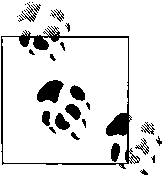
\includegraphics[width=2cm,clip]{paipai.png}
\end{wrapfigure}
\mbox{}\begin{flushleft}是的,这个函数名的确少个e。 Ken Thompson,Unix的创建者,曾开玩笑说漏掉这个字母是他设计Unix中最后悔的事情。\end{flushleft} 
\par
典型的creat()调用如下: 
\begin{lstlisting}
  int fd;
  fd = creat (file, 0644);
  if (fd == -1)
      /* error */
\end{lstlisting}

等价于: 

\begin{lstlisting}
  int fd;

  fd = open (file, O_WRONLY | O_CREAT | O_TRUNC, 0644);
  if (fd == -1)
      /* error */
\end{lstlisting}

即使可以在用户空间上简单creat()的功能,但是在大部分Linux架构上\footnote[1]{回忆一下,系统调用是在每种架构基础上定义的。 就是说,像i386有creat()系统调用,而Alpha则没有。你可以在任意架构上使用creat(),当然,可能它只是一个库函数而不是个系统调用。},creat()是一个系统调用: 

\begin{lstlisting}
  int creat (const char *name, int mode)
  {
      return open (name, O_WRONLY | O_CREAT | O_TRUNC, mode);
  }
\end{lstlisting}

这是一个历史遗留问题,由于从前open()只有两个参数,所以才导致现在的重复。现在,creat()系统调用仍为了兼容性而保留。 在新架构中可以像glibc里那样实现creat()。 

\subsection{返回值和错误码}

open()和creat()调用成功时都返回一个文件描述符。错误时都返回-1,并将errno设置为一个合适的错误值(第一章讨论了errno,并列出了可能的错误值)。处理文件打开的错误并不复杂,一般来说,在取消的打开文件操作前不需要什么处理,典型的方式是提示用户换个文件或终止程序。 

\section{用read()读取文件}

现在你知道了如何打开文件,我们来看该如何读取它。 在接下来的一节,我们将讨论写操作。

最基本、也是最常见的读取文件的机制是使用read()系统调用。该系统调用在POSIX.1中定义如下: 

\begin{lstlisting}
  #include <unistd.h>

  ssize_t read (int fd, void *buf, size_t len);
\end{lstlisting}

该系统调用从由fd指向的文件的当前偏移量至多读len个字节到buf中。 成功时,将返回写入buf中的字节数。出错时则返回-1,并设置errno。 fd所指文件位置指针将会向前移动,移动的长度由之前读取的字节数决定。如果无法在该文件(比如一个字符设备文件)中确定文件位置,读操作总是从“当前”位置开始。

基本用法很简单。 下面的例子从fd所指的文件中读取数据并保存到word中。 读取字节数等于unsigned long类型的大小,在32位Linux系统上是4字节,而在64位系统则是8字节。 返回时,nr保存读取字节数,如果出错,则nr为-1: 

\begin{lstlisting}
  unsigned long word;
  ssize_t nr;
  /* read a couple bytes into 'word' from 'fd' */
  nr = read (fd, &word, sizeof (unsigned long));
  if (nr == -1)
      /* error */
\end{lstlisting}
这个不成熟的实现有两个问题:调用可能没有读完len个字节就返回,而且可能产生某些这段代码本身没有检查和处理的错误。 不幸的是,像这样的代码非常普遍。 我们来看看如何改进它。

\subsection{返回值}

返回一个比len小的非零正整数对于read()来说是合法的。 出现这种情况,可能有各种各样的原因,例如:可供读取的字节数本来就比len要少,系统调用可能被信号打断,管道可能被破坏(如果fd是个管道),等等。

另外一种需要考虑的是调用read()时返回0的情况。当已位于文件尾时,read()系统调用返回0,说明已经到达文件结尾(EOF);这种情况下,当然没有字节被读入。 EOF并不是一种错误(也因此不用返回-1);它仅仅表示文件位置指针已经位于文件最后一个有效偏移量之后,之后没有任何数据可读了。然而,如果一个调用需要读len个字节,但却没一个字节可读,调用将阻塞(睡眠),直到那些字节可以读取为止(假设文件描述符没有在非阻塞模式下打开;参见“非阻塞读取”)。 注意这与返回EOF时不同。 就是,“没有数据可读”和“数据末尾”是不同的。 在EOF的情况下,到达了文件末尾。在阻塞的情况下,读操作在等待更多的数据--例如在从套接字或者设备文件读取的时候。

有些错误是可以恢复的。比如,当read()调用在未读取任何字节前被一个信号打断,它会返回-1(如果为0,则可能和EOF混淆),并设置errno为EINTR。在这种情况下,你可以重新提交读取请求。

对read()的调用确实会有很多可能的结果:
\begin{itemize}
\item 调用返回一个等于len的值。所有len个被读取字节存储在buf中。结果和预期一致。

\item 调用返回了一个大于零但小于len的值。读取的字节存入buf中。这种情况出现在一个信号打断了读取过程,或在读取中发生了一个错误,有效字节大于零,但比len字节少时,或者在读入len个字节前已抵达EOF。再次进行读取(更新了buf和len的值)将读入剩余字节到buf的剩余空间中,或者指出问题发生的原因。
\item 调用返回0。这标志着EOF。没有可以读入的数据。

\item 调用阻塞了,因为没有可用的用来读取的数据。这在非阻塞模式下不会发生。

\item 调用返回-1,并且errno被设置为EINTR。这表示在读入字节之前收到了一个信号。可以重新进行调用。

\item 调用返回-1,并且errno被设置为EAGAIN。这表示读取会因没有可用的数据而阻塞,而读请求应该在之后重开。这只在非阻塞模式下发生。

\item 调用返回-1,并且errno被设置不同于EINTR或EAGAIN的值。这表示某种更严重的错误。

\end{itemize}
\subsection{读入所有的字节}

如果你想要处理所有的错误,并且读入所有len个字节(至少读到EOF),那么之前简单的read()是不合适的。 为了达到目的,你需要一个循环,和一些条件语句。 

\begin{lstlisting}
  ssize_t ret;

  while (len != 0 && (ret = read (fd, buf, len)) != 0) {
      if (ret == -1) {
          if (errno == EINTR)
              continue;
          perror ("read");
          break;
  }
      len -= ret;
      buf += ret;
  }
\end{lstlisting}

这段代码处理了所有五种情况。循环从fd所指的当前文件位置读入len个字节到buf中,读入会一直到读完所有len个字节或者到EOF为止。如果读入了多于零个但少于len个字节,从len中减去已读字节数,buf增加相应数量的字节数,并重新调用read()。如果调用返回了-1,并且errno等于EINTR,将重新调用且不更新参数。如果调用返回-1,且errno被设置为其他值,将调用perror()来向标准错误打印一条描述并终止循环。

部分读入不仅是合法的,还是常见的。无数bug就是由于程序员没有正确检查处理较短读入请求而产生的。请不要成为其中一员! 

\subsection{非阻塞读}

有时候,程序员不希望当没有可读数据时让read()调用阻塞。相反,他们倾向于在没有可读数据时,让调用立即返回。这种情况被称为非阻塞I/O;它允许应用在从不阻塞的状况下进行I/O操作,如果是在操作多个文件时,不至于丢失其他文件中的可用数据。

所以,还有一个errno的值需要检查:EAGAIN。像先前讨论的那样,如果给出的文件描述符在非阻塞模下打开(open()中给定O\_NONBLOCK; 参见“open()的flags参数”)并且没有可读数据,read()调用会返回-1,且设置errno为EAGAIN而不是阻塞掉。在进行非阻塞I/O时,你必须检查EAGAIN,否则将可能因导数据缺失而导致严重的错误。你可能会用到下面的代码: 

\begin{lstlisting}
  char buf[BUFSIZ];
  ssize_t nr;
  start:
  nr = read (fd, buf, BUFSIZ);
  if (nr == -1) {
      if (errno == EINTR)
          goto start; /* oh shush */
      if (errno == EAGAIN)
          /* resubmit later */
      else
          /* error */
  }
\end{lstlisting}
\par
\begin{wrapfigure}{l}{2.5cm}
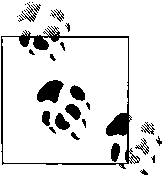
\includegraphics[width=2cm,clip]{paipai.png}
\end{wrapfigure}
\mbox{}\begin{flushleft}在处理EAGAIN时使用一个goto start可能实际上没什么意\\义---你大概只需要不使用非阻塞I/O即可。使用它并不能\\节省时间,相反还引入了更多的循环带来的开销。\end{flushleft} 


\subsection{其他错误码}
其他的错误代码表示编程错误或者(对EIO来说)底层问题。在read()失败后可能的errno值包括: 

\begin{eqlist*}
\item [EBADF]
给出的文件描述符非法,或者不是用可读方式打开的。 
\item [EFAULT]
buf指针不在调用进程的地址空间内。
\item [EINVAL]
文件描述符对应的对象不允许读取。 
\item [EIO]
发生了一个底层I/O错误。
\end{eqlist*}

\subsection{read()大小限制}
size\_t和ssize\_t类型由POSIX确定。size\_t类型用来存储用字节衡量大小的值。ssize\_t类型是有符号的size\_t类型(负值用来表示错误)。在32位系统上,对应的C类型一般分别是unsigned int和int。由于两种类型常常一起使用,ssize\_t的较小范围就潜在地给size\_t的范围作出了限制。

size\_t的最大值为SIZE\_MAX;ssize\_t的最大值为SSIZE\_MAX。如果len比SSIZE\_MAX 大,read()调用的结果是未定义的。在大部分Linux系统上,SSIZE\_MAX是LONG\_MAX,在32位系统上即0x7fffffff。这个数字对一次读入来说已经足够大了,但还是需要记住它。如果你要用前面的读循环代码作为一种通用的读取方式,你可能需要增加如下代码:

\begin{lstlisting}
  if (len > SSIZE_MAX)
      len = SSIZE_MAX;
\end{lstlisting}

一个len为零的read()调用的结果是立即返回且返回值为0。 

\section{用write()来写}

最常见的写文件的系统调用是write()。 write()与read()相对应,也在POSIX.1中定义。 

\begin{lstlisting}
  #include <unistd.h>

  ssize_t write (int fd, const void *buf, size_t count);
\end{lstlisting}

一个write()调用从由文件描述符fd引用文件的当前位置开始,将buf中至多count个字节写入文件中。 不支持定位的文件(像字符设备)总是从“开头”开始写。

成功时,返回写入字节数,并更新文件位置。错误时,返回-1,并将errno设置为相应的值。一个write()可以返回0,但这种返回值没有任何特殊含义;只是表示写入了零个字节。

像read()一样,最基本的用法很简单: 

\begin{lstlisting}
  const char *buf = "My ship is solid!";
  ssize_t nr;
 
  /* write the string in 'buf' to 'fd' */
  nr = write (fd, buf, strlen (buf));
  if (nr == -1)
      /* error */
\end{lstlisting}

与read()仍然相像的是,这种简单用法并不大合适。调用者也需要检查出现部分写的各种可能情况。

\begin{lstlisting}
  unsigned long word = 1720;
  size_t count;
  ssize_t nr;

  count = sizeof (word);
  nr = write (fd, &word, count);
  if (nr == -1)
      /* error, check errno */
  else if (nr != count)
      /* possible error, but 'errno' not set */
\end{lstlisting}

\subsection{部分写}

相对于read()的返回部分读的情况,write()不太可能返回一个部分写的结果。而且,对write()系统调用来说没有EOF情况。对于普通文件,除非发生一个错误,否则write()将保证写入所有的请求,。

那么,对于普通文件,你就不需要进行循环写了。然而对于其他类型——例如套接字——大概得有个循环来保证你真的写入了所有请求的字节。使用循环的另一个好处是,第二次write()调用可能会返回一个错误值用来说明第一次调用为什么进行了一次部分写(尽管这种情况不大常见)。请大家看下面的示例代码:

\begin{lstlisting}
  ssize_t ret, nr;

  while (len != 0 && (ret = write (fd, buf, len)) != 0) {
      if (ret == -1) {
          if (errno == EINTR)
              continue;
          perror ("write");
          break;
      }
      len -= ret;
      buf += ret;
  }
\end{lstlisting}

\subsection{追加模式}

当fd在追加模式下打开时(通过指定O\_APPEND参数),写操作就不从文件描述符的当前位置开始,而是从当前文件末尾开始。

举例来说,假设有两个进程在向同一个文件写。不使用追加模式的话,如果第一个进程向文件末尾写,而第二个进程也这么做,那么第一个进程的文件位置将不再指向文件末尾,而将指向文件末尾减去第二个进程写入的字节数的地方。这意味着多个进程如果不进行显式的同步则不能进行追加写操作,因为它们存在竞争条件。

追加模式避免了这样的问题。它保证文件位置总是指向文件末尾,这样所有的写操作总是追加的,即便有多个写者。你可以认为每个写请求之前的文件位置更新操作是原子操作。文件位置更新至刚刚写入的数据结尾。这和下一个write()调用无关,因为更新文件位置是自动完成的,但可能因为某些奇怪的原因会影响到下一个read()调用。

追加模式在某些任务中很管用,像更新日志文件,但在不少其他方面也没什么用处。

\subsection{非阻塞写}
当fd在非阻塞模式下打开时(通过设置O\_NONBLOCK参数),并且发起的写操作会正常阻塞时,write()系统调用返回-1,并设置errno值为EAGAIN。请求应该在稍后重新发起。通常处理普通文件时不会出现这种事。 

\subsection{其他错误码}
其他值得注意的错误值包括:
\begin{eqlist*}
\item [EBADF]
给定的文件描述符非法,或者不是以写方式打开的。 
\item [EFAULT]
buf指针指向不在进程地址空间内。 
\item [EFBIG]
写操作将使文件大小超过进程的最大文件限制,或者内部实现的限制。 
\item [EINVAL]
给定的文件描述符对应的对象不能用来进行写操作。 
\item [EIO]
发生了一个底层I/O错误。 
\item [ENOSPC]
文件描述符所在的文件系统没有足够的空间。 
\item [EPIPE]
给定文件描述符关联的管道或套接字的读端被关闭。进程也将收到一个SIGPIPE信号。SIGPIPE信号的默认行为是终止收到信号的进程。因而,进程只能在选择忽略,阻塞或者处理该信号时得到这个值。 
\end{eqlist*}

\subsection{write()大小限制}

如果count比SSIZE\_MAX还大,write()调用的结果是未定义的。 count值为零的write()调用将立即返回且返回值为0。 

\subsection{write()的行为}
当一个write()调用返回时,内核已将所提供的缓冲区数据复制到了内核缓冲区中,但却没有保证数据已写到目的文件。write调用返回对于这样的情况来讲确实得太快了。处理器与硬盘的速度差异使这种情况非常明显。

当用户空间应用发起write()系统调用时,Linux内核进行几项检查,然后直接将数据拷贝至一个缓冲区中。稍后,在后台,内核收集所有这样的“脏"缓冲区,将它们排好序,并写入到磁盘上(此过程称为回写)。这使得write调用马上被调用并立刻返回。内核可以将写入操作推迟到空闲阶段,并将很多写操作一起处理。

这种延迟写不会改变POSIX所定义的语义。举例来说,如果一个read调用希望读取刚刚写到缓冲区中但尚未写入磁盘的数据,请求将从缓冲区中响应,而不是读取磁盘上“陈旧”的数据。这种行为实际上提高了效率,因为read只需从内存缓存中读而不用到硬盘中找。读写请求如预计般交错,而结果也如预期那样——当然,前提是在数据写入磁盘前,系统没有崩溃!在这种情况下,即使对于一个应用程序来讲写操作已经成功了,但数据并没有写入到磁盘。

另外一个关于延迟写的问题是对强制写顺序的不可能性。尽管一个应用可能会注意安排它的写请求以使它们将按特定顺序写入磁盘,出于性能方面的考虑,内核将按它觉得合适的顺序重新安排。在系统崩溃时才是问题,而最终所有缓冲区都将正确地写回。尽管如此,绝大多数的应用实际上并不关心写顺序。

最后一个延迟写的问题是关于特定I/O错误的报告。任何在回写中出现的I/O错误——比方说,一个物理磁盘驱动器错误——不会被报告给发起写请求的进程。实际上,缓冲区是和进程完全无关的。多进程可能会更新同一片缓冲区中的数据,而进程可能在数据仍在缓冲区未回写到磁盘前就退出了。另外,你怎么才能在事后与一个写操作失败的进程通讯呢?

内核会尝试将延迟写的风险最小化。为保证数据适时写入,内核创立了一种缓存最大时效机制,并将所有脏的缓存在它们超过给定时效前写入磁盘。用户可以通过/proc/sys/vm/dirty\_expire\_centiseconds来配置这个值。这个值以十毫秒计(百分之一秒)。

强制文件缓存写回也是可以的,甚至可以将所有的写操作同步。这些将是下一节讨论的主题,“同步I/O。”

在本章后面部分,“内核内幕”将深入探讨Linux内核的缓冲回写子系统。 

\section{同步I/O}

尽管同步I/O是一个重要的主题,但不必担心和延迟写相关的问题。由于写缓冲提供了巨大的性能改进,以至于一些半吊子的“现代”系统都用缓冲区实现了延迟写。然而,常有应用想要控制数据被写入磁盘的时间。对于这些需要,Linux内核提供了一些选择来允许用性能换取同步操作。 

\subsection{fsync()和fdatasync()}

最简单的确认数据写入磁盘的方法是使用fsync()系统调用,它在POSIX.1b中定义如下:

\begin{lstlisting}
  #include <unistd.h>

  int fsync (int fd);
\end{lstlisting}

调用fsync()可以保证fd对应文件的脏数据回写到磁盘上。文件描述符fd必须是以写方式打开的。该调用回写数据以及建立的时间戳和inode中的其他属性等元数据。在驱动器确认数据已经全部写入之前不会返回。

在将数据写入硬盘缓存时,fsync()是不可能知道数据是否已经在磁盘上了。磁盘可能报告说数据已写入,但数据可能还在磁盘驱动器的缓存上。幸运的是,在磁盘驱动器缓存中的数据将会很快写入到磁盘。

Linux还提供了fdatasync()系统调用:

\begin{lstlisting}
  #include <unistd.h>

  int fdatasync (int fd);
\end{lstlisting}

这个系统调用完成的事情和fsync()一样,区别在于它仅写入数据。该调用不保证元数据同步到磁盘上,故此可能快一些。一般来说这就够了。

两个函数有相同的用法,非常简单: 

\begin{lstlisting}
  int ret;

  ret = fsync (fd);
  if (ret == -1)
      /* error */
\end{lstlisting}

这两个调用都不保证任何已经更新的包含该文件的目录项同步到磁盘上。这意味着如果文件链接刚刚被更改过,文件数据可能会成功写入磁盘,但却没有关联到相应的目录项上,致使文件不可访问。 为保证任何对目录项的更新也同步到磁盘上,必须对目录本身也调用fsync()进行同步。

\subsection{返回值和错误码}

成功时,两个调用都返回0。失败时,都返回-1,并将errno设置为以下三个值之一:

\begin{eqlist*}
\item [EBADF]
给定的文件描述符不是一个可以写入的合法描述符。 
\item [EINVAL]
给定的文件描述符对应的对象不支持同步。
\item [EIO]
在同步时发生了一个底层I/O错误。这表示一个真正的I/O错误,此类错误经常在错误发生处被捕获。
\end{eqlist*}

一般来讲,即使在相应文件系统上实现了fdatasync()而未实现fsync(),在调用fsync()时也会失败。“偏执”的应用可能会在fsync()返回EINVAL时尝试用fdatasync(),如下所示:

\begin{lstlisting}
  if (fsync (fd) == -1) {
      /*
      * We prefer fsync(), but let's try fdatasync( )
      * if fsync( ) fails, just in case.
      */
      if (errno == EINVAL) {
          if (fdatasync (fd) == -1)
          perror ("fdatasync");
      } else
          perror ("fsync");
  }
\end{lstlisting}

在POSIX标准中fsync()是必要的,而fdatasync()是可选的,因此fsync()在所有常见的、面向普通文件的Linux文件系统都已经实现了。然而,特殊文件类型(可能是那些没有元数据需要同步的文件类型)或者不常见的文件系统或许只实现了fdatasync()。 

\subsection{sync()}

sync()系统调用可以用来对磁盘上的所有缓冲区进行同步,尽管其效率不高,但仍然被广泛使用:

\begin{lstlisting}
  #include <unistd.h>

  void sync (void);
\end{lstlisting}

该函数没有参数,也没有返回值。它总是成功返回,并确保所有的缓冲区——包括数据和元数据——都能写入磁盘。\footnote[1]{好吧,和以往一样,为防止误解在此加以说明:硬盘可能会撒谎,它通知内核缓冲区已经写到磁盘上了,但实际上它们仍在磁盘缓存中。}

标准中并不要求sync()一直等待到所有缓冲区都写到磁盘才返回;只需要调用它来启动将整个将缓冲区写入磁盘的过程即可。由此,一般建议同步多次以确保所有的数据都安全的写入磁盘。然而对于Linux来讲,sync()一定要等到所有的缓冲区都写入才返回。因而,调用一次sync()就够了。

sync()真正派上用场的地方是在工具sync的实现中。应用程序则使用fsync()和fdatasync()将文件描述符指定的数据同步到磁盘。需要注意的是,可能在一个繁忙的系统上sync()操作可能需要几分钟的时间来完成。 

\subsection{O\_SYNC标志}

O\_SYNC标志在open()中使用,使所有在文件上的I/O操作同步。

\begin{lstlisting}
  int fd;

  fd = open (file, O_WRONLY | O_SYNC);
  if (fd == -1) {
      perror ("open");
      return -1;
  }
\end{lstlisting}

读请求总是同步的。如果不同步,将无法保证读取缓冲区中数据的有效性。然而,像先前讨论的那样,write()调用一般是非同步的。调用返回和数据写入磁盘之间没有什么关系。O\_SYNC标志则强制将二者关联,从而保证write()调用进行I/O同步。

O\_SYNC看起来就像是在每个write()操作后都隐式地执行fsync()。尽管这在语法上是毫无问题的,但Linux内核实现的O\_SYNC会更有效一点。

O\_SYNC将在写操作中稍稍影响用户及内核时间(分别为在用户和内核空间消耗的时间)。此外,根据写入文件的大小,可能会使大量的时间消耗在进程的I/O 等待时间(用来等待I/O完成的时间)上,此时的O\_SYNC会使总耗时增加一到两个数量级。这种时间开销增长是非常可观的,所以同步I/O一般是在无计可施情况下的最后选择。

一般情况下,需要确保数据写入磁盘的应用可以使用fsync()或者fdatasync()。因为需要较少的调用(比如,只在某个决定性的操作完成之后),相对于O\_SYNC来讲,开销也更少。 

\subsection{O\_DSYNC和O\_RSYNC}

POSIX为open()定义了另外两个同步相关的标志:O\_DSYNC和O\_RSYNC。在Linux上,这些标志与O\_SYNC同义;它们有相同的行为。


O\_DSYNC标志指定在每次写操作后只有普通数据被同步,元数据则不同步。这看起来就像是在每个写请求后隐式调用fdatasync()一样。因为 O\_SYNC提供了更好的保证,所以没有明确支持O\_DSYNC时并不会导致功能缺失;只是在O\_SYNC有更强要求的情况下有一点性能损失。


O\_RSYNC标志要求读请求像写请求那样进行同步。因此,该标志只能和O\_SYNC或O\_DSYNC一起使用。如前文所述,读操作总是同步的——直到有数据需要返回给用户的时候才会返回。O\_RSYNC标志保证任何读操作的副作用也是同步的。这意味着从一个读操作来更新元数据也须是在调用返回前写入磁盘。实际中,这差不多是要求在read()调用返回前,文件访问时间必须更新到磁盘上的inode中。尽管没有多少意义,Linux还是将O\_RSYNC设定为与O\_SYNC一样(与O\_SYNC和O\_DSYNC的关系不同)。在Linux中通常无法确知O\_RSYNC 的行为;对开发者而言最接近的方式是在每个read()调用后调用fdatasync()。实际上,极少需要这种操作。 

\section{直接I/O}

与其他现代操作系统内核一样,Linux内核实现了一个复杂的缓存、缓冲以及设备和应用之间的I/O管理的层次结构(参见本章末尾“内核内幕”)。一个高性能应用可能希望越过这些复杂的层次结构并进行独立的I/O管理。和I/O系统做斗争实在没什么必要,事实上操作系统层次的工具往往比应用层工具有更好的性能。然而,数据库系统还是倾向于使用他们自己的缓存,以尽可能的减少操作系统的影响。

在open()中使用O\_DIRECT标志会使内核最小化I/O管理的影响。使用该标志时,I/O操作将忽略页缓存机制,直接对用户空间缓冲区和设备进行初始化。所有的I/O将是同步的;操作在完成之前不会返回。

当使用直接I/O时,请求长度,缓冲区对齐,和文件偏移必须是设备扇区大小(通常是512字节)的整数倍。在2.6内核之前,要求更严格:在2.4中,所有的东西都必须对齐到文件系统逻辑块大小(一般是4KB)。为保持兼容性,应用需要对齐到更大的(而且更不便的)逻辑块大小。

\section{关闭文件}

程序完成对某个文件的操作后,可以使用close()系统调用将文件描述符和对应的文件解除关联。

\begin{lstlisting}
  #include <unistd.h>

  int close (int fd);
\end{lstlisting}

close()调用解除了已打开的文件描述符的关联,并分离进程和文件的关联。给定的文件描述符不再有效,内核可以随意将其作为随后的open() 或creat()调用的返回值而重新使用。close()调用在成功时返回0。而错误时返回-1,并设置errno为相应值。用法很简单:

\begin{lstlisting}
  if (close (fd) == -1)
      perror ("close");
\end{lstlisting}

需要注意的是,关闭文件和文件被写入磁盘没什么关系。如果应用想保证文件在关闭前写到磁盘,需要使用一个先前在“同步I/O”中讨论的同步选项。

然而关闭文件的确有些副作用。当最后一个引用某文件的文件描述符关闭后,在内核中表示该文件的数据结构就被释放了。当它释放时,与文件关联的inode的内存拷贝被清除。如果没有什么连接到该inode了,它可能会从内存中清除(也有可能保留在内存中,因为内核为了效率缓存一些inode,但也可能不需要)。如果文件已经从磁盘上解除链接,但在解除前仍保持打开,它在被关闭且inode从内存中移除前就不会真的被删除。因而,对 close()的调用可能会使某个已解除链接的文件最终从磁盘上被删除。

\subsection{错误码}

一个常见的错误是不检查close()的返回值。这样处理可能会忽略了某个重大的错误。某些操作因为延迟的原因,其错误可能在后来才出现,而close()会报告这些错误。

以下是一些在出错时可能出现的errno 值。除了EBADF(给定的文件描述符不合法),最重要的错误值是EIO,这个错误值表明一个可能和实际的close操作并不相关的底层I/O错误。如果忽略出现的错误,文件描述符合法的情况下,总是会被关闭的,并且与其关联的数据结构被释放。

尽管POSIX允许,但close()绝不会返回EINTR。Linux内核开发者们可能很清楚,这样的实现并不明智。

\section{用lseek()查找}

一般的,一个文件中的I/O是线性的,由读写引发的文件位置的隐式更新就是全部需要查找定位的了。然而一些应用需要在文件中跳来跳去。lseek()系统调用能够对给定文件描述符引用的文件位置设定指定值。除了更新文件位置,没有其它的行为,并不初始化任何I/O。 

\begin{lstlisting}
  #include <sys/types.h>
  #include <unistd.h>

  off_t lseek (int fd, off_t pos, int origin);
\end{lstlisting}

lseek()的行为依赖于初始参数,可以为以下值之一:
\begin{eqlist*}
\item [SEEK\_CUR]
当前文件位置fd设置为当前值加上pos,pos可以为负值,零或正值。一个为零的pos返回当前文件位置值。
\item [SEEK\_END]
当前文件位置fd设置为当前文件长度加上pos,pos可以为负值,零或正值。一个为零的pos设置偏移量为文件末尾。
\item [SEEK\_SET]
当前文件位置fd设置为pos。一个为零的pos设置偏移量为文件起始。
\end{eqlist*}

调用在成功时返回新文件位置。错误时返回-1并设置适当的errno值。

举例设置文件位置fd为1825: 

\begin{lstlisting}
  off_t ret;

  ret = lseek (fd, (off_t) 1825, SEEK_SET);
  if (ret == (off_t) -1)
      /* error */
\end{lstlisting}

或者,设置文件位置fd到文件末尾: 

\begin{lstlisting}
  off_t ret;

  ret = lseek (fd, 0, SEEK_END);
  if (ret == (off_t) -1)
      /* error */
\end{lstlisting}

由于lseek()返回更新过的文件位置,可以用SEEK\_CUR和零值来确定文件当前位置:

\begin{lstlisting}
  int pos;

  pos = lseek (fd, 0, SEEK_CUR);
  if (pos == (off_t) -1)
      /* error */
  else
      /* 'pos' is the current position of fd */
\end{lstlisting}

显然,lseek()最常见的用法是来定位一个文件描述符的开始和末尾,或是确定该描述符的当前文件位置。 

\subsection{文件末尾之后进行查找}

lseek()是可以在文件指针超过文件末尾之后进行查找的。举例来说,下面的代码将查找到fd对应的文件末尾之后1688个字节。 

\begin{lstlisting}
  int ret;

  ret = lseek (fd, (off_t) 1688, SEEK_END);
  if (ret == (off_t) -1)
      /* error */
\end{lstlisting}

对这种用法本身来说,查找到文件末尾之后没什么影响——到最新产生的文件位置的读请求会返回EOF。然而如果在接下来对该位置有一个写请求,则会在新旧长度之间建立新的空间,并由零来填充。

这种零填充方式称为“空洞”(hole)。在Unix风格的文件系统上,空洞不占用任何物理上的磁盘空间。这暗示着文件系统上所有文件的大小加起来可以超过磁盘的物理大小。带空洞的文件叫做“稀疏文件”(sparse file)。稀疏文件可以节省可观的空间并提升效率,因为操作那些空洞并不引发任何物理I/O。

一个对文件空洞部分的读请求将返回相应数量的二进制零。 

\subsection{错误码}

出错时,lseek()返回-1,并将errno设置为下面四个之值之一: 

\begin{eqlist*}
\item [EBADF]
给出的文件描述符没有指向任何打开的文件。
\item [EINVAL]
origin的值不是SEEK\_SET,SEEK\_CUR或者SEEK\_END其中之一,或者最终计算的文件位置为负数。事实上,如果出现EINVAL的这两种错误都是很不幸的。前者几乎肯定是一个编译时的错误,而后者可能代表一个隐蔽得多的运行时逻辑错误。
\item [EOVERFLOW]
计算后的文件偏移不能被off\_t表示。这种情况只会发生在32位架构上。当前,文件位置会被修改;而这个错误只是表示不能返回这个值。
\item [ESPIPE]
给出的文件描述符关联到了一个不能执行查找操作的对象上,例如管道,FIFO或套接字。
\end{eqlist*}

\subsection{限制}

文件位置的上限值被限定为off\_t类型的大小。大部分架构定义这个值为C的long类型,在Linux上总是字长(通常是机器通用寄存器的大小)。从内部实现来看,内核将偏移量存储成C的long long类型。这种处理方法在64位机器上没有问题,但在32位机器上作相应查找时可能产生EOVERFLOW错误。 

\section{定位读写}

Linux提供了两种read()和write()的变体来替代lseek(),每个调用都以需要读写的文件位置为参数。完成时,不修改文件位置。

读形式的调用为pread():

\begin{lstlisting}
  #define _XOPEN_SOURCE 500

  #include <unistd.h>

  ssize_t pread (int fd, void *buf, size_t count, off_t pos);
\end{lstlisting}

这个调用从文件描述符fd的pos文件位置读取count个字节到buf中。

写形式的调用为pwrite():

\begin{lstlisting}
  #define _XOPEN_SOURCE 500

  #include <unistd.h>

  ssize_t pwrite (int fd, const void *buf, size_t count, off_t pos);
\end{lstlisting}

这个调用从文件描述符fd的pos文件位置写count个字节到buf中。

除了它们不管当前文件位置,这些调用的行为和read()、wirte()几乎没有区别,它们使用pos提供的值而不是当前位置。此外,在调用完成时,它们不会修改文件位置。换句话说,任何混杂的read()和write()调用可能破坏了定位读写的结果。

两种定位读写调用都只能用于可以进行定位操作的文件描述符。从语义角度来讲,相当于在调用read()或write()前使用 lseek()进行定位,但有仍有三点区别:第一,这些调用更加简单易用,尤其是在文件中做反向移动和随机移动这种技巧性很强的操作时更是如此。第二,当操作完成时,不修改文件位置指针。最后,也是最重要的,避免了任何在使用lseek()时可能出现的潜在竞争。由于线程共享文件描述符,可能在一个线程调用lseek()之后,但尚未进行读写操作前,另一个线程修改文件位置。我们可以通过使用pread()和pwrite()来避免产生这样的竞争。 

\subsection{错误码}

成功时,两个调用返回读或写的字节数。pread()返回零表示EOF;而对pwrite(),一个零值返回表明调用没有写任何东西。出错时,二者均返回-1并设置errno为相应值。对pread()而言,任何对read()或lseek()的errno值都是可能出现的。对pwrite()而言,任何 write()或lseek()的errno值也都是可能出现的。 

\section{截短文件}

Linux提供了两个系统调用来截短文件,二者都在各类POSIX标准中定义并(不同程度的)实现。 它们分别是:

\begin{lstlisting}
  #include <unistd.h>
  #include <sys/types.h>

  int ftruncate (int fd, off_t len);
\end{lstlisting}

和:

\begin{lstlisting}
  #include <unistd.h>
  #include <sys/types.h>

  int truncate (const char *path, off_t len);
\end{lstlisting}

两个系统调用都将文件截短到len指定的长度。ftruncate()系统调用操作一个打开的并且可写的文件描述符fd。truncate()系统调用操作path指定的一个可写文件。二者都在成功时返回0。错误时返回-1,并设置errno为相应值。

这两个系统调用最常见的用途是将文件截短到比原文件长度小一些。成功返回时,文件长度变成len。之前在len和旧长度之间的数据将被忽略,并不可读取。

它们也可以将文件“截短”到比原长度更长,类似于前面“查找到文件末尾之后”中查找加上写操作的结合。扩展出的字节将全部填充为零。

这两个操作均不修改当前文件位置。

举例来看,考虑包含下面内容的74字节大小的文件pirate.txt:

\begin{verbatim}
  Edward Teach was a notorious English pirate.

  He was nicknamed Blackbeard.
\end{verbatim}

从同一个路径下,运行下面的程序: 

\begin{lstlisting}
  #include <unistd.h>
  #include <stdio.h>
  int main( )
  {
      int ret;

      ret = truncate ("./pirate.txt", 45);
      if (ret == -1) {
          perror ("truncate");
          return -1;
      }
      return 0;
  }
\end{lstlisting}

结果产生了包含如下45字节的文件:

\begin{verbatim}
  Edward Teach was a notorious English pirate. 
\end{verbatim}

\section{I/O多路复用}

应用程序常常需要在多于一个文件描述符上阻塞:例如响应键盘输入(stdin)、进程间通信以及同时操作多个文件。基于事件驱动机制的图形用户界面(GUI)应用的主循环中可能包含上百个等待响应的事件。\footnote[1]{主循环对于任何写过GUI应用的人来说是很熟悉的了——像GNOME用一个由GLib,它的基本库提供的主循环。一个主循环允许从一个阻塞点开始监控多个事件并响应。}

在不使用线程,尤其是独立处理每一个文件的情况下,进程无法在多个文件描述符上同时阻塞。如果文件都处于准备好被读写的状态,同时操作多个文件描述符是没有问题的。但一旦在该过程中出现一个未准备好的文件描述符(就是说,如果一个read()被调用,但没有读入数据),则这个进程将会阻塞,不能再操作其他文件。可能阻塞只有几秒钟,但是应用无响应也会造成不好的用户体验。然而,如果该文件描述符始终没有任何可用数据,就可能一直阻塞下去。文件描述符的I/O总是相关的(例如管道),很可能一个文件描述符依赖另外一个文件描述符,直到后者可以被使用前,前者一直处于不可用状态。尤其是对网络应用程序而言,同时打开的多个套接字,会诱发潜在的问题。

试想一下如下场景:当标准输入设备挂起,无数据输出,应用在一个进程间通信相关的文件描述符上阻塞。应用只有在阻塞的IPC文件描述符返回数据后,才能确知键盘输入已经挂起。如果被阻塞的操作没有返回,情况又会怎样呢?

如前所述,非阻塞I/O 可以作为这个问题的一个解决方案。使用非阻塞I/O,应用可以发起I/O请求并返回一个特别的错误,从而避免阻塞。从两个方面来讲,这种方法效率较差。首先,进程需要以某种不确定的方式不断发起I/O操作,直到某个打开的文件描述符准备好进行I/O。这种设计很糟糕。其次,如果程序可以睡眠的话将更加有效,可以让处理器进行其他工作,直到一个或更多文件描述符可以进行I/O时再唤醒。

进入I/O多路复用。

I/O多路复用允许应用在多个文件描述符上同时阻塞,并在其中某个可以读写时收到通知。这时I/O多路复用就成了应用的关键所在,一般来讲I/O多路复用的设计遵循以下原则: 

\begin{enumerate}
\item I/O多路复用:当任何文件描述符准备好I/O时告诉我
\item 在一个或更多文件描述符就绪前始终处于睡眠状态。
\item 唤醒:哪个准备好了?
\item 在不阻塞的情况下处理所有I/O就绪的文件描述符。
\item 返回第一步,重新开始。 
\end{enumerate}

Linux提供了三种I/O多路复用方案:select,poll和epoll。我们先看看前两个,我们将在第四章讨论最后一个,那是Linux特有的高级方法。 

\subsection{select()}

select()系统调用提供了一种实现同步I/O多路复用的机制: 

\begin{lstlisting}
  #include <sys/time.h>
  #include <sys/types.h>
  #include <unistd.h>

  int select (int n,
 	      fd_set *readfds,
	      fd_set *writefds,
	      fd_set *exceptfds,
	      struct timeval *timeout);
  FD_CLR(int fd, fd_set *set);
  FD_ISSET(int fd, fd_set *set);
  FD_SET(int fd, fd_set *set);
  FD_ZERO(fd_set *set);
\end{lstlisting}

在指定的文件描述符准备好I/O之前或者超过一定的时间限制,select()调用就会阻塞。

监测的文件描述符可以分为三类,分别等待不同的事件。监测readfds集合中的文件描述符,确认其中是否有可读数据(也就是说,读操作可以无阻塞的完成)。监测writefds集合中的文件描述符,确认其中是否有一个写操作可以不阻塞地完成。监测exceptefds中的文件描述符,确认其中是否有出现异常发生或者出现带外(out-of-band)数据(这种情况只适用于套接字)。指定的集合可能为空(NULL),相应的,select()则不对此类时间进行监视。

成功返回时,每个集合只包含对应类型的I/O就绪的文件描述符。举例来说,readfds集合中有两个文件描述符:7和9。当调用返回时,如果7还在集合中,该文件描述符就准备好进行无阻塞I/O了。如果9已不在集合中,它可能在被读取时会发生阻塞。(我这里说“可能”是因为数据可能在调用完成后已经就绪了。在这种情况下,下一个select()调用返回时,将该文件描述符返是就绪的。\footnote[1]{这是因为select()和poll()都是电平触发而不是边沿触发的。将在第四章讨论的epoll(),可以在任一种方式下工作。边沿触发操作简单一些,但允许在未注意时错过I/O事件。})

第一个参数n,等于所有集合中文件描述符的最大值加一。这样,select()的调用者需要找到最大的文件描述符值,并将其加一后传给第一个参数。

timeout参数是一个指向timeval结构体的指针,定义如下: 

\begin{lstlisting}
 #include <sys/time.h>

 struct timeval {
	long tv_sec; /* seconds */
	long tv_usec; /* microseconds */
 };
\end{lstlisting}

如果这个参数不是NULL,即使此时没有文件描述符处于I/O就绪状态,select()调用也将在tv\_sec秒tv\_usec微秒后返回。返回时,这个结构体的状态在大多俗话Unix系统中都是未定义的。这样的话,每次调用前都必须重新初始化(还有集合中的文件描述符)。较新版本的Linux会自动将该值改为剩余的时间。这样,如果时限是5秒,在某个文件描述符准备好时过去了3秒,tv.tv\_sec在返回时就还是2。

如果时限中的两个值都是零,调用会立即返回,并报告调用时所有事件对应的文件描述符均不可用,且不等待任何后续事件。

集合中的文件操作符并不直接操作,而是通过辅助宏来进行管理。这就允许Unix系统按其所希望的方式来实现,大多数系统,将其实现为位数组。FD\_ZERO从指定集合中移除所有文件描述符。在每次使用select()之前,需要调用该宏。 

\begin{lstlisting}
  fd_set writefds;
 
  FD_ZERO(&writefds);
\end{lstlisting}

FD\_SET向指定集合中添加一个文件描述符,而FD\_CLR从指定集合中移除一个文件描述符。 

\begin{lstlisting}
  FD_SET(fd, &writefds); /* add 'fd' to the set */
  FD_CLR(fd, &writefds); /* oops, remove 'fd' from the set */
\end{lstlisting}

设计良好的代码应该从不使用FD\_CLR。一般来讲,很少使用该宏。

FD\_ISSET测试一个文件描述符在不在给定集合中。如果在,则返回一个非零值,否则用0表示不在。一般在select()调用返回后使用FD\_ISSET来检查一个文件描述符是否就绪。 

\begin{lstlisting}
  if (FD_ISSET(fd, &readfds))
      /* 'fd' is readable without blocking! */
\end{lstlisting}

由于文件描述符集合是静态建立的,所以对于文件描述符数量的上限和文件描述符的最大值均有限制,二者都由FD\_SETSIZE设定。在Linux上,这个值是1024。我们将在本章稍后来看看这个限制的作用。 

\subsection{返回值和错误码}

成功时,select()返回在所有三个集合中I/O就绪的文件描述符的数目。如果给出了时限,返回值可能为0。错误时返回-1,而且errno被设置为下列值之一: 

\begin{eqlist*}
\item [EBADF]
某一个集合中的一个文件描述符非法。
\item [EINTR]
等待时捕获了一个信号,可以重新发起调用。
\item [EINVAL]
参数n是负数,或者给出的时限不合法。
\item [ENOMEM]
没有足够的内存完成请求。
\end{eqlist*}

\subsubsection{select()示例程序}

我们来看看下面的样例程序,虽然简单但是对select()用法的介绍却非常完整。这个例子中,等待stdin的输入的阻塞时限设置为5秒钟。由于只监测了一个文件描述符,实际上这不是I/O多路复用,但系统调用的用法却很清晰。 

\begin{lstlisting}
  #include <stdio.h>
  #include <sys/time.h>
  #include <sys/types.h>
  #include <unistd.h>

  #define TIMEOUT 5 /* select timeout in seconds */
  #define BUF_LEN 1024 /* read buffer in bytes */

  int main (void)
  {
      struct timeval tv;
      fd_set readfds;
      int ret;
      /* Wait on stdin for input. */
      FD_ZERO(&readfds);
      FD_SET(STDIN_FILENO, &readfds);
      /* Wait up to five seconds. */
      tv.tv_sec = TIMEOUT;
      tv.tv_usec = 0;
      /* All right, now block! */
      ret = select (STDIN_FILENO + 1,
		    &readfds,
		    NULL,
		    NULL,
		    &tv);
      if (ret == -1) {
          perror ("select");
          return 1;
      } else if (!ret) {
          printf ("%d seconds elapsed.\n", TIMEOUT);
          return 0;
      }

      /*
       * Is our file descriptor ready to read?
       * (It must be, as it was the only fd that
       * we provided and the call returned
       * nonzero, but we will humor ourselves.)
       */
      if (FD_ISSET(STDIN_FILENO, &readfds)) {
          char buf[BUF_LEN+1];
	  int len;
	  /* guaranteed to not block */
	  len = read (STDIN_FILENO, buf, BUF_LEN);
	  if (len == -1) {
	      perror ("read");
	      return 1;
	  }
	  if (len) {
	      buf[len] = '\0';
	      printf ("read: %s\n", buf);
          }
          return 0;
      }

      fprintf (stderr, "This should not happen!\n");
      return 1;
  }
\end{lstlisting}

\subsubsection{用select()实现可移植的sleep()}

由于select()在各种Unix系统中都很容易实现,相对于微秒级精度的睡眠机制来讲,经常将select()做为一种可移植的微秒级的睡眠机制。该方法通过将三个集合值设为空(NULL),将超时值设置为非空(non-NULL)来实现。 

\begin{lstlisting}
  struct timeval tv;

  tv.tv_sec = 0;
  tv.tv_usec = 500;

  /* sleep for 500 microseconds */
  select (0, NULL, NULL, NULL, &tv);
\end{lstlisting}

当然,Linux提供了高精度的睡眠机制的实现,具体内容,我们将在第十章中学习。

\subsubsection{pselect()}

在4.2BSD中首次引入的select()很受欢迎,但POSIX定义了自己的方法——pselect(),在POSIX 1003.1g-2000和后来的POSIX 1003.1-2001中对pselect()做了如下定义: 

\begin{lstlisting}
  #define _XOPEN_SOURCE 600
  #include <sys/select.h>

  int pselect (int n,
      fd_set *readfds,
      fd_set *writefds,
      fd_set *exceptfds,
      const struct timespec *timeout,
      const sigset_t *sigmask);

  FD_CLR(int fd, fd_set *set);
  FD_ISSET(int fd, fd_set *set);
  FD_SET(int fd, fd_set *set);
  FD_ZERO(fd_set *set);
\end{lstlisting}

pselect()和select()有三点不同:

1. pselect()的timeout参数使用了timespec结构,而不是timeval结构。timespec使用秒和纳秒,不是秒和毫秒,从理论上来讲更精确一些。实际上,两者在毫秒精度上已经都不可靠了。

2. pselect()调用并不修改timeout参数。这个参数在后续调用时也不需要重新初始化。

3. select()调用没有sigmask参数。当这个参数被设置为零时,pselect()的行为等同于select()。

timespec结构体定义为如下形式: 

\begin{lstlisting}
  #include <sys/time.h>

  struct timespec {
      long tv_sec; /* seconds */
      long tv_nsec; /* nanoseconds */
  };
\end{lstlisting}

添加pselect()到Unix工具箱的主要原因是为了增加sigmask参数,以此来解决信号和等待文件描述符之间的竞争条件(信号在第九章深入讨论)。假设一个信号处理程序设置了一个全局标记(大部分信号处理程序都这么干),进程在每次调用select()前都要检查这个标记。现在,假如在检查标记和调用之间接收到信号,应用可能会阻塞,并不再响应该信号。pselect()提供了一组可阻塞的信号,可以解决这个问题。阻塞的信号直到解除阻塞才会被处理。一旦pselect()返回,内核就恢复旧的信号掩码。详见第九章。

2.6.16内核之前,Linux实现的pselect()还不是一个系统调用,而是由glibc提供的一个简单的对select()的封装。该方法使竞争条件出现的风险最小化,但是没有根本消除。当真正引入一个系统调用,才彻底解决竞争问题。

如果不考虑pselect()中(相对不大的)改进,大多数应用会继续使用select(),部分是出于习惯,其他则是考虑可移植性。

\subsection{poll()}

poll()系统调用是System V的I/O多路复用解决方案。它解决了一些select()的不足,不过select()仍经常被使用(还是出于习惯和可移植性的考虑):

\begin{lstlisting}
  #include <sys/poll.h>

  int poll (struct pollfd *fds, unsigned int nfds, int timeout);
\end{lstlisting}

与select()使用的三个基于位掩码的文件描述符集合不同,poll()使用一个简单的nfds个pollfd结构体构成的数组,fds指向该数组。结构体定义如下:

\begin{lstlisting}
  #include <sys/poll.h>

  struct pollfd {
      int fd; /* file descriptor */
      short events; /* requested events to watch */
      short revents; /* returned events witnessed */
  };
\end{lstlisting}

每个pollfd结构体指定监视单一的文件描述符。可以传递多个结构体,使得poll()监视多个文件描述符。每个结构体的events字段是要监视的文件描述符事件的一组位掩码。用户设置这个字段。revents字段则是发生在该文件描述符上的事件的位掩码。内核在返回时设置这个字段。所有在 events字段请求的事件都可能在revents字段中返回。下面是合法的事件: 

\begin{eqlist*}
\item [POLLIN]
有数据可读。 
\item [POLLRDNORM]
有正常数据可读。
\item [POLLRDBAND]
有优先数据可读。
\item [POLLPRI]
有高优先级数据可读。
\item [POLLOUT]
写操作不会阻塞。
\item [POLLWRNORM]
写正常数据不会阻塞。
\item [POLLBAND]
写优先数据不会阻塞。
\item [POLLMSG]
有一个SIGPOLL消息可用。
\end{eqlist*}

另外,如下事件可能在revents中返回: 

\begin{eqlist*}
\item [POLLER]
给出文件描述符上有错误。
\item [POLLHUP]
文件描述符上有挂起事件。
\item [POLLNVAL]
给出的文件描述符非法。
\end{eqlist*}

这些在events中没有意义,而总是在合适时返回。使用poll(),不像select()那样,你无需另外请求报告异常。 

POLLIN | POLLPRI等价于select()的读事件,而POLLOUT | POLLWRBAND等价于select()的写事件。POLLIN等价于POLLRDNORM | POLLRDBAND,而POLLOUT等价于POLLWRNORM。

举例来说,监视一个文件描述符是否可读写,我们需设置events为POLLIN | POLLOUT。返回时,我们将在revents中是否有相应的标志。如果设置了POLLIN,文件描述符就需要能非阻塞读。如果设置了POLLOUT,文件描述符需要能非阻塞写。这些标志并不相互排斥:二者都可以设置,表示可以在文件描述符上读写,并都不会阻塞。

timeout参数指定在任何I/O就绪前需要等待时间的长度,以毫秒计。负值表示永远等待。一个零值表示调用立即返回,列出所有未准备好的I/O,但不等带任何其他事件。这种情况下,poll()就如同其名,轮询一次后立即返回。 

\subsubsection{返回值和错误码}

成功时,poll()返回具有非零revents字段的文件描述符个数。超时前没有任何事件发生则返回零。失败时返回-1,errno被设置为下列值之一: 

\begin{eqlist*}
\item [EBADF]
一个或更多结构体中有非法的文件描述符。
\item [EFAULT]
指向fds的指针超出了进程地址空间。 
\item [EINTR]
在请求事件发生前收到了一个信号,可以重新调用。
\item [EINVAL]
nfds参数超过了RLIMIT\_NOFILE值。 
\item [ENOMEM]
没有足够的内存完成请求。
\end{eqlist*}

\subsubsection{poll()的例子}

我们来看一个使用poll()的样例程序,要同时检测一个stdin读和一个stdout写是否阻塞: 

\begin{lstlisting}
  #include <stdio.h>
  #include <unistd.h>
  #include <sys/poll.h>

  #define TIMEOUT 5 /* poll timeout, in seconds */

  int main (void)
  {
      struct pollfd fds[2];
      int ret;

      /* watch stdin for input */
      fds[0].fd = STDIN_FILENO;
      fds[0].events = POLLIN;
      /* watch stdout for ability to write (almost always true) */
      fds[1].fd = STDOUT_FILENO;
      fds[1].events = POLLOUT;

      /* All set, block! */
      ret = poll (fds, 2, TIMEOUT * 1000);
      if (ret == -1) {
          perror ("poll");
          return 1;
      }

      if (!ret) {
          printf ("%d seconds elapsed.\n", TIMEOUT);
          return 0;
      }

      if (fds[0].revents & POLLIN)
          printf ("stdin is readable\n");

      if (fds[1].revents & POLLOUT)
          printf ("stdout is writable\n");

      return 0;
  }
\end{lstlisting}

运行,我们得到了预期的结果:

\begin{verbatim}
  $ ./poll

  stdout is writable
\end{verbatim}

再次运行,但将一个文件重定向到标准输入,我们看到了两个事件:

\begin{verbatim}
  $ ./poll < ode_to_my_parrot.txt

  stdin is readable

  stdout is writable
\end{verbatim}

假设我们在一个应用中使用了poll(),我们无需在每次调用时重新构建pollfd结构体。相同的结构可能会被反复传递;必要时内核会把revents字段清空。 

\subsubsection{ppoll()}

Linux提供了一个poll()的近似调用——ppoll()。ppoll()和pselect()同源,然而和pselect()不同的是,ppoll()是Linux的专有调用:

\begin{lstlisting}
  #define _GNU_SOURCE
  #include <sys/poll.h>

  int ppoll (struct pollfd *fds,
             nfds_t nfds,
	     const struct timespec *timeout,
	     const sigset_t *sigmask);
\end{lstlisting}

像pselect()那样,timeout参数以秒和纳秒计指定了时限,而sigmask参数提供了一组等待处理的信号。 

\subsection{poll()与select()}

尽管它们完成一样的工作,但poll()系统调用仍然优于select(): 

\begin{itemize}
\item \begin{flushleft}poll()无需使用者计算最大的文件描述符值加一和传递该参数。\end{flushleft}
\item \begin{flushleft}poll()在应对较大值的文件描述符时更具效率。想像一下用select()监视值为900的文件描述符——内核需要检查每个集合中的每个比特位,直到第九百个。\end{flushleft}
\item \begin{flushleft}select()的文件描述符集合是静态大小的,所以要作出权衡:要么集合很小,限制了select()可以监视的文件描述符的最大值,要么较大,但是效率不高。尤其是当不能确定集合的组成是否稀疏时,对较大位掩码的操作效率不高。\footnote[1]{如果位掩码是稀疏组成的,每个带有掩码的字都可以用零来检测;只在操作返回失败值时需要对每个位进行检测。然而这项工作很浪费,如果位掩码比较稠密的话。}使用poll()则可以创建合适大小的数组。只需要监视一项或仅仅传递一个结构体。\end{flushleft}
\item \begin{flushleft}若用select(),文件描述符集合会在返回时重新创建,这样的话之后每个调用都必须重新初始化它们。poll()系统调用分离了输入(events字段)和输出(revents字段),数组无需改变即而重用。\end{flushleft}
\item \begin{flushleft}select()的timeout参数在返回时是未定义的。可移植的代码需要重新初始化它。然而pselect()没有这个问题。\end{flushleft}
\end{itemize}

但是select()系统调用的确有几个不错的地方:

\begin{itemize}
\item \begin{flushleft}poll()由于某些Unix系统不支持poll(),所以select()的可移植性更好。\end{flushleft}
\item \begin{flushleft}select()提供了更好的超时方案:直到微秒级。ppoll()和pselect()在理论上都提供纳秒级的精度,但在实际中,没有任何调用可以可靠的提供哪怕是微秒级的精度。\end{flushleft}
\end{itemize}

比poll()和select()更好的是epoll接口,一个Linux特有的I/O多路复用解决方案,我们将在第四章探讨。

\section{内核内幕}

这部分来看看Linux内核是如何实现I/O的,集中关注三个主要的内核子系统:虚拟文件系统(VFS),页缓存,和页回写。这些子系统使Linux中的I/O看起来无缝运转,且更加高效。 

\begin{wrapfigure}{l}{2.5cm}
  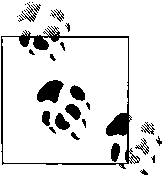
\includegraphics[width=2cm,clip]{paipai.png}
\end{wrapfigure}
\mbox{}在第四章,我们将看到第四个子系统,I/O调度器。 

\subsection{虚拟文件系统}

虚拟文件系统(有时也叫做virtual file switch)是一种Linux内核的文件操作的抽象机制。它允许内核在无需了解文件系统类型的情况下,使用文件系统函数和操作文件系统数据。

VFS实现这种抽象的方法是使用一种通用文件模型(common file model),它是所有Linux文件系统的基础。基于函数指针和各种面向对象方法\footnote[1]{是的,在C中。},通用文件模型提供了一种Linux内核文件系统必须遵循的框架。它允许VFS对文件系统发起请求。框架提供了钩子来支持读,建立链接,同步以及其他功能。每种文件系统再使用合适的函数来处理相应操作。

这种方法强制要求文件系统间需要有一定的共性。举个例子,VFS工作于inode,superblock和目录条目之上。一个非Unix 的文件系统可能缺少类Unix的概念如inodes,只不过需要去处理解决。确实如此:Linux可以很好的支持像FAT和NTFS这样的文件系统。

VFS的好处太多了。一个简单的系统调用可以从任意媒介上的任意文件系统上读;一个简单的工具可以从一个文件系统拷贝到另一个上。所有文件系统都支持同样的概念,同样的接口,和同样的调用。一切都正常工作——而且工作得很好。

当一个应用发起一个read()系统调用,就开始了一段奇妙的旅程。C库提供了系统调用的定义,而在编译器调用转化为适当的陷阱态。当一个用户空间进程转入内核态,则转交系统调用处理器处理,最终交给read()系统调用,内核确认文件描述符所对应的对象类型。然后内核调用与相关类型对应的 read()函数。对于文件系统而言,这个函数是文件系统代码的一部分。然后该函数继续其工作——举例来说,从文件系统中读取数据——并把数据返回给用户空间的read()调用,该调用返回复制数据到用户空间的系统调用处理器,然后将数据复制到用户空间,最后read()系统调用返回而进程继续执行。

对系统程序员来说,VFS的影响是很重要的。程序员不需担心文件所在的文件系统或者介质。通用系统调用——read(),write(),以及其他——能够在任意支持的文件系统和介质上操作文件。 

\subsection{页缓存}

页缓存是一种在内存中保存最近在磁盘文件系统上访问过的数据的方式。相对于现在的处理器速度而言,磁盘访问速度过慢。在内存中保存被请求数据,内核在接下来对相同数据的后续请求可以直接从内存中读取,尽量避免重复磁盘访问。

页缓存利用了引用局部性(locality of reference)的一种方法——时间局部性(temporal locality),该方法使刚被访问资源很可能会在不久后再次被访问。由于避免了费时的磁盘访问,内存在第一次访问时缓存数据的开销因而得到补偿

页缓存是内核寻找文件系统数据的第一目的地。只有缓存中找不到时内核才会调用存储子系统从磁盘中读取数据。当数据第一次读取后,就会从磁盘读入页缓存中,并从缓存中返回给应用。如果那项数据被再次读取,就直接从缓存中返回。通过页缓存的所有操作执行都是透明的,保证它的数据总是相关且有效的。

Linux页缓存大小是动态的。随着I/O操作将越来越多的数据带入内存,页缓存也随之增大,消耗掉空闲的内存。如果页缓存最终确实消耗掉了所有的空闲内存,而且有新增的存储要求出现,页缓存就会被削减,释放它最少使用的页,将空间让给“真正的”内存使用。这种处理是自动进行的。一个动态变化的缓存允许Linux使用所有的系统内存,并缓存尽可能多的数据。

向磁盘交换一块很少使用的数据,比从页缓存中清除掉一条常常使用的且很可能将在下次重读中使用的数据更有意义(交换允许内核在磁盘上存储数据,得到比机器的RAM更大的内存空间)。Linux内核实现了一些平衡交换数据和清理页缓存(以及其他驻存项目)的启发式方法。这些启发式方法可能会决定用交换数据到磁盘来代替清理页缓存,尤其是在交换的数据并未使用时。

交换和缓存间的平衡可以通过 /proc/sys/vm/swappiness 来调整。这个文件可以在0到100间取值,默认为60。较高的值表示倾向于在内存中保留页缓存,较低的值表示更倾向于清理页缓存而不是进行交换。

引用局部性(locality of reference)的另一种形式是空间局部性(sequential locality),是关于数据的连续使用的性质。基于这个原理,内核实现了页缓存预读技术。预读是在每次读请求时从磁盘数据中读取更多的数据到页缓存中的动作——多读一点点会很有效。当内核从磁盘读取一块数据时,也会读取接下来一两块数据。一次读取较大的连续数据块时磁盘不需要经常寻道,所以会比较有效,。另外,内核可以在进程操作第一块读取数据时完成预读。像经常发生的那样,如果进程继续对接下来的块提交一个新的读请求,内核就可以不用发起磁盘 I/O而直接将预读数据转交。

和页缓存类似,内核管理预读也是动态的。如果它注意到一个进程持续使用预读来的数据,内核就会增加预读窗口,因而预读进更多的数据。预读窗口最小为16KB,最大128KB。反之,如果内核发现预读没有造成任何有用的命中——就是说,应用在文件中来回查找而不是连续的读——它可以完全关闭预读。

页缓存的存在对程序员来讲是透明的。系统程序员一般来说不需要优化代码以期从页缓存机制中得到更多好处(除非是在用户空间实现这样一种缓存)。一般的,有效率的代码就是以最大限度利用页缓存。另一方面,利用预读也不错。虽然不总是如此,但多数情况下连续文件I/O通常多于随机访问。 

\subsection{页回写}

像先前在“write()的行为”中讨论的那样,内核使用缓冲区来延迟写操作。当一个进程发起写请求,数据被拷贝进一个缓冲区,并将该该缓冲区标记为" 脏"的,这意味着内存中的拷贝要比磁盘上的新。此时,写请求就可以返回了。如果对同一个数据块有新的写请求,缓冲区就更新为新数据。在该文件其他部分的写请求则开辟新的缓冲区。 

最终那些"脏"缓冲区需要写入磁盘,将磁盘文件和内存数据同步。这就是所谓的回写。以下两个条件会触发回写: 

\begin{itemize}
\item \begin{flushleft}当空闲内存小于设定的阈值时,脏的缓冲区就会回写到磁盘上,被清理的缓冲区可能会被移除,来释放内存空间。\end{flushleft}
\item \begin{flushleft}当一个脏的缓冲区寿命超过设定的阈值时,缓冲区被回写至磁盘。以此来避免数据的不确定性。 \end{flushleft}
\end{itemize}

回写由一些叫做pdflush的内核线程操作(推测可能是page dirty flush之意,但谁知道呢)。当以上两种情况之一出现时,pdflush线程被唤醒,并开始将脏的缓冲区提交到磁盘,直到没有触发条件被满足。

可能同时有多个pdflush线程在回写。这么做是为了更好的利用并行性而避免拥塞。拥塞避免机制确保在等待向某个块设备进行写操作时,其他的写操作不被积压下来。如果来自其他块设备有脏缓冲区存在,其他pdflush线程就会充分利用每一块设备。这改良了以前内核的一处不足:先前的pdflush线程(bdflush,一个单一线程)可能要消耗掉所有的时间来等待一个块设备,而同时其他块设备处于空闲。在一台现代机器上,Linux内核现在可以使许多个磁盘维持饱和状态。

缓冲区在内核中使用buffer\_head结构来表示。这个数据结构跟踪各种各样与缓冲区关联的元数据,例如缓冲区是干净的还是脏的。同时,它也维护了一个指向实际数据的指针。这部分数据保存在页缓存中。用这样的方式,将缓冲子系统和页缓存统一了起来。

在早期Linux内核版本中——2.4之前——缓冲子系统与页缓存是分离的,这样就同时有一个页缓存和一个缓冲缓存。这意味着数据可以同时在缓冲缓存(作为脏的缓冲区)和页缓存(用来缓存数据)之中存在。自然的,同步这两块缓存要用一些时间。在2.4 Linux内核中引入的统一的页缓存,这是一个不错的改进。

Linux中的延迟写和缓冲子系统可以使写操作迅速完成,代价是要冒着在电源故障时出现数据丢失的风险。为避免这种风险,关键性应用可以使用同步I/O(在本章先前讨论过)。 

\section{结论}

这一章讨论了Linux系统编程的基础:文件I/O。在Linux这样一个一切皆文件的操作系统中,知道如何打开,读,写和关闭文件是非常重要的。所有这些操作都是传统的Unix方式,在多种标准中都有谈及。

下一章集中处理缓冲I/O,以及标准C库的标准I/O接口。标准C库不仅仅是出于方便考虑;用户空间的缓冲I/O提供了关键的性能提升。 



\ifx\atempxetex\usewhat
\XeTeXinputencoding "utf-8"
\fi
\defaultfont

\chapter{缓冲输入输出}

  让我们来回顾一下第一章中的块的概念,做为文件系统的抽象,它是I/O中最基本的概念-所有的磁盘操作都是基于块进行的。因此,当请求以块大小整数倍对齐地址时,I/O效率是最理想的。

  操作效率随着系统调用次数的增多而急剧下降。例如,每次读一字节读1024次与一次读1024字节相比,显然后者效率更优。如果长度不是 block(块)的整数倍,即使每次以大于块的长度进行一系列的操作,其效率也不是最理想的。例如块的大小是1K,每次以1130字节的长度操作数据要比每次1024字节的速度慢。 

\section{用户-缓冲I/O}
  需要对普通文件执行许多轻量级I/O请求的程序通常使用用户缓冲I/O。用户缓冲I/O是在用户空间而不是在内核中完成的,它可以在程序中设定,也可以调用标准库透明地执行。正如第二章中讨论的,出于性能方面的考虑,内核通过延迟写操作,组合相邻I/O请求和预读等操作来缓冲数据。通过不同的方法,用户缓冲的主旨也是为了提高操作效率。

以用户空间程序dd为例:
\begin{lstlisting}
  dd bs=1 count=2097152 if=/dev/zero of=pirate
\end{lstlisting}

因为参数bs=1,这个命令会进行2,097,152次操作(每次一字节)从文件/dev/zero(一个提供无限的0文件流的虚拟设备)中拷贝2M到文件 pirate中。也就是说,拷贝文件的过程会产生大约2百万次的读写操作——每次一个字节。

现在考虑相同的2M字节拷贝,但是每次使用1024字节的块:
\begin{lstlisting}
  dd bs=1024 count=2048 if=/dev/zero of=pirate
\end{lstlisting}

该操作复制相同的2M 字节内容到相同的文件中,但是前一种方式执行的读写操作次数是该种方式的1024倍。正如你在表3-1中看到的,效率提高是很显著的。表中记录了用四个只在每次拷贝块大小上有区别的 dd命令所耗费的时间(用三种不同的测量)。实际时间是总消耗的时钟时间,用户时间是在用户空间中执行程序代码的时间,而系统时间是指进程在内核中执行系统调用所消耗的时间。

表3-1. 块大小对性能的影响

\begin{tabular}{cccc}
Block size  &  Real time     & User time    &  System time\\ \hline
1 byte    &   18.707 seconds &  1.118 seconds & 17.549 seconds\\
1,024 bytes &   0.025 seconds  & 0.002 seconds & 0.023 seconds\\
1,130 bytes  &  0.035 seconds  & 0.002 seconds & 0.027 second\\
\end{tabular}



使用1024字节块大小进行操作和1字节块相比,获得了巨大的性能提升。但是,这个表也显示用一个更大的块大小(这也意味着较少的系统调用),如果块大小不是磁盘块大小的整数倍,那么会导致效率变差。即使需要更少的调用,1130字节的请求导致产生不对齐的操作,因此比1024字节的请求效率更低。

为了利用这个特性,需要预先知道可能的物理块大小。表中显式的结果表明块大小最可能是1024,1024的整数倍,或者是1024的约数。在本例中,/dev/zero的块大小实际上是4096B。

\subsection{块大小}

实际应用中,块大小一般是512字节, 1024字节, 2048字节, 或4096字节。如表3-1中显示,效率的大规模提升只是通过将每次操作的数据设置为块大小整数倍或约数获得的。这是因为内核和硬件之间是通过块交互的。所以,使用块大小或者一个能够恰好能放入一个块中的值来保证请求是块对齐的,可以防止无关的内核操作。

通过用系统调用stat()(我们将在第七章讨论)或stat(1)可以轻松指定设备的块大小。 事实上,一般情况下我们不需要知道确切的块大小.

为I/O操作选择一个大小的主要目标是不要选择像1130这样一个莫名其妙的值。Unix的历史上没有块长度是1130字节的,选择这样的块大小会在第一次操作后导致I/O不对齐。但是使用块大小的整数倍或约数就可以防止不对齐的请求。只要你选择的大小保持所有操作块对齐, 效率就会好。较大的整数倍只是减少了系统调用次数。

然而,最简单的方法是用一个大小为标准块大小整数倍的缓冲区来执行I/O。 4096或8192字节的效果都不错.

但问题是程序很少以块为单位进行操作.程序往往以区域,行,和单个字符为单位进行操作,而不是抽象的块。如前所述,为了改善这种情况,程序使用用户缓冲I/O. 当数据被写入时,它会被存储在程序地址空间的缓冲区中。当缓冲区规模达到一个给定的值(缓冲区大小时),整个缓冲区会在一次操作中被写出。同理,读操作一次读入缓冲区大小且块对齐的数据。当应用程序执行不对齐的读请求时,缓冲区一块一块的给出数据。最后,当缓冲区为空时,另一个大的块对齐的区域又被读入。如果缓冲区的大小设置得当,将会有很大的效率提升。

你可以在程序中实现用户缓冲。事实上很多关键应用就是独立实现用户缓冲的。然而大部分程序使用标准I/O库(C标准库的一部分),这个库可以提供健壮而且功能强大的用户缓冲方案。

\subsection{标准I/O}

C标准库中提供了标准I/O库(通常简单称作stdio),其中实现了一个跨平台用户缓冲的解决方案。这个标准I/O库使用简单,而且功能强大。与其他编程语言(例如FORTAN)不同, 除了流控制和算数运算等基本支持外,C语言并没有对其他高级功能提供内嵌支持,当然也没有对I/O的内在支持。随着C语言的发展,用户们开发了一些提供核心功能的函数,例如字符串处理、数学函数库、日期时间库以及I/O库等。随着这些例程日渐成熟,在ANSI C委员会的许可下(C89),这些函数最终被归入C语言标准库。虽然C95和C99都加入了一些新的接口,标准I/O库与1989年刚刚创建的时候相比改变不大。

本章余下的部分讨论用户缓冲I/O。因为它属于文件输入输出,而且在C标准库中实现,因此打开、关闭、读写文件都是通过C标准库完成。一个程序究竟应该使用标准I/O或是自创的用户缓冲,还是直接使用系统调用,这些都需要设计者仔细权衡程序的需求和行为后才能决定。

C标准通常会给每种实现保留一些的细节,而相关实现通常会加入一些扩展的特性。本章和本书的其它章节一样,主要讨论现代Linux上的接口和行为,这些接口和行为主要是用glibc实现的。在Linux偏离基本标准的时候,我们会予以指明。

\subsection{文件指针}

标准I/O例程并不直接操作文件描述符。取而代之的是它们用自己唯一的标志符,即大家熟知的文件指针(file pointer)。在C标准库里,文件指针映射到一个文件描述符。文件指针由FILE类型的指针表示,FILE类型定义在<stdio.h>中。

在标准I/O中,一个打开的文件叫做"流"(stream)。 流可以被打开用来读(输入流), 写(输出流),或者二者兼有(输入输出流)。 

\section{打开文件}

文件通过fopen()打开以供读写操作:
\begin{lstlisting}
  #include <stdio.h>
  FILE* fopen(const char * path, const char * mode);
\end{lstlisting}

这个函数根据指定的模式打开文件path,并为它关联一个新的流。

\subsection{模式}

参数模式mode描述以怎样的方式打开指定文件。 它可以是下述字符串之一:
\begin{list}{}
\item \textbf{r}\\
   打开文件用来读取。流定位在文件的开始处。
\item \textbf{r+}\\
   打开文件用来读写。流定位在文件的开始处。
\item \textbf{w}\\
   打开文件用来写入,如果文件存在, 文件会被清空。 如果文件不存在,它会被创建。流定位在文件的开始处。
\item \textbf{w+}\\
   打开文件用来读写。如果文件存在,文件会被清空。如果文件不存在,它会被创建。流被设置在文件的开始。
\item \textbf{a}\\
   打开文件用来追加模式的写入。如果文件不存在它会被创建。流被设置在文件的末尾。所有的写入都会接在文件后。
\item \textbf{a+}\\
   打开文件用来追加模式的读写。如果文件不存在,它会被创建。流被设置在文件的末尾。 所有的写入都会接在文件后。
\end{list}
给定的模式可能还有字符b,但这个值在Linux下通常会被忽略。 一些操作系统用不同的方式对待文本和二进制文件, 并且b模式指示文件用二进制打开。Linux, 和所有的符合可移植性的操作系统,以相同的方式对待文本和二进制文件。

成功时,fopen()返回一个合法的FILE指针。 失败时,它返回NULL,而且相应的设置errno。

例如,下面的代码打开/etc/manifest以供读取,并将它与一个流关联:
\begin{lstlisting}
  FILE *stream;
  stream = fopen ("/etc/manifest", "r");
  if (!stream)
    /* error */
\end{lstlisting}


\subsection{通过文件描述符打开文件}

函数fdopen()将一个已经打开的文件描述符(fd)转成一个流:
\begin{lstlisting}
  #include <stdio.h>
  FILE * fdopen (int fd, const char *mode);
\end{lstlisting}

fdopen()的可能模式和fopen()一样,而且必许和原来打开文件描述符的模式匹配。可以指定模式w和w+,但是它们不会截断文件。流的位置设置在文件描述符指向的文件位置。 一旦文件描述符被转换为一个流, 则不应该直接在该文件描述符上进行I/O(尽管这么做是合法的)。需要注意的是文件描述符没有被复制,而只是关联了一个新的流。关闭流也会关闭相应的文件描述符。成功时,fdoepn()返回一个合法的文件指针;失败时,返回NULL。 例如, 下面的代码通过open()系统调用打开/home/kidd/map.txt,然后用已有的文件描述符创建一个关联的流:
\begin{lstlisting}
  FILE *stream;
  int fd;
  fd = open ("/home/kidd/map.txt", O_RDONLY);
  if (fd == −1)
    /* error */
  stream = fdopen (fd, "r");
  if (!stream)
   /* error */
\end{lstlisting}


\section{关闭流}

fclose()函数关闭一个给定的流:
\begin{lstlisting}
  #include <stdio.h>
  int fclose (FILE *stream);
\end{lstlisting}


所有被缓冲但还没有被写出的数据会被先写出。成功时,fclose()返回0。失败时返回EOF并且相应的设置errno。

\subsection{关闭所有的流}

fcloseall()函数关闭所有的和当前进程相关联的流,包括标准输入,标准输出,标准错误:
\begin{lstlisting}
  #define _GNU_SOURCE
  #include <stdio.h>
  int fcloseall (void);
\end{lstlisting}

关闭之前,所有的的流会被写出。这个函数始终返回0;该函数是Linux所特有的。 

\section{从流中读取数据}

C标准库实现了多种从流中读取数据的方法。这部分会考察三种最常用的:单个字节的读取,单行的读取,和二进制数据读取。为了从流中读数据,流必须以恰当的方式打开;也就是说,任何除了w或a的模式都可以。

\subsection{单字节读取}

通常,理想的输入输出模式是每次简单地读取一个字符。函数fgetc()可以用来从流中读取单个字符:
\begin{lstlisting}
  #include <stdio.h>
  int fgetc (FILE *stream);
\end{lstlisting}

这个函数从流中读取下一个字符并把该无符号字符强转为int返回。强转是为了有足够的范围来表示文件结尾符和错误:在这种情况下EOF会被返回。fgetc()的返回值必须以int型保存。把返回值保存为char类型中是一个很常见但很危险的错误。下面的例子从流中读取单个字符,检查错误,然后以字符方式打印结果:
\begin{lstlisting}
  int c;
  c = fgetc (stream);
  if (c == EOF)
    /* error */
  else
    printf ("c=%c\n", (char) c);
\end{lstlisting}

stream指向的流必须以可读模式打开。

\subsection{把字符回放入流中}

标准输入输出提供了一个将字符放回流中的函数。这个函数允许你“偷窥”流,如果你不需要该字符的话,可以把它放回。
\begin{lstlisting}
  #include <stdio.h>
  int ungetc (int c, FILE *stream);
\end{lstlisting}

每次调用把c强转成一个无符号字符并放回流中。成功时,返回c;失败时返回EOF。随后读取流会返回c。如果多个字符被放入流中,它们会以倒序的方式返回-就是说,最后推入的先返回。POSIX 指出,在中间没有读入请求时只能保证一次放回成功。然而有些实现只允许一次放回。只要有足够的内存,Linux允许无限次数的放回。一次放回当然总会成功。

如果你在调用ungetc()之后,但在执行下一个读入请求之前执行了一次定位函数(见本章后半部分'定位流')的调用,会导致所有推回的字符被丢弃。在一个进程的多个线程中确实是这样的,因为所有的线程共享一个缓冲区。

\subsection{按行的读取}

函数fgets()从一个给定的流中读取一个字符串:
\begin{lstlisting}
  #include <stdio.h>
  char * fgets (char *str, int size, FILE *stream);
\end{lstlisting}

这个函数从流中读取 size-1 个字节的数据,并把数据存入str中。 当所有字节读入时,空字符被存入字符串末尾。当读到EOF或换行符时读入结束。如果读到了一个换行符,'{\textbackslash}n'被存入str。

成功时返回str;失败时,返回NULL。例如:
\begin{lstlisting}
  char buf[LINE_MAX];
  if (!fgets (buf, LINE_MAX, stream))
    /* error */
\end{lstlisting}

POSIX 在<limits.h>中定义了宏LINE\_MAX:它是POSIX行控制接口能够处理的输入行的最大长度。linux的C函数库没有提供这样的限制(行可以是任意长度),但是不能和宏LINE\_MAX交互。可移植程序可以用LINE\_MAX来保证安全;在linux系统中,该值被设置的相对较高。针对linux的程序无需担心行大小的限制。

\subsection{读取任意字符串}

fgets()基于行的读取通常是很有用的。但很多时候它又很麻烦。有时候开发者想用一个分隔符而不是换行符。有时候开发者根本不需要一个分隔符-而且极少数情况下开发者希望分隔符留在缓冲区。从历史经验来看,在返回的缓冲区中存入换行符很少是正确的。

用fgetc()写一个fgets()并不难。例如,下面的代码片段从流中读取n-1个字节到str中,然后加上一个'\textbackslash0':
\begin{lstlisting}
  char *s; 
  int c;
  s = str;
  
  while (--n > 0 && (c = fgetc (stream)) != EOF)
    *s++ = c;
    *s = '\0';
\end{lstlisting}

这段程序可以扩展为在任意指定的分隔符 d 处停止(在本例中d不能是空字符):
\begin{lstlisting}
  char *s;
  int c = 0;
  s = str;
  
  while (--n > 0 && (c = fgetc (stream)) != EOF && (*s++ = c) != d)
    ;
  if (c == d)
    *--s = '\0';
  else
    *s = '\0';
\end{lstlisting}

除了在缓冲区中存入换行符,将d设置为'{\textbackslash}n'可以提供和fgets()类似的功能,。

根据fgets()的实现,这个实现方式可能要慢些,因为它重复调用了很多次fgetc()。 然而,这和我们一开始的dd例子不同。虽然这段代码出现了过多的函数调用,但它没有进行过多的系统调用和dd程序中bs=1引起的不对齐I/O负担,相对来讲后者是更大的问题。

\subsection{读取二进制文件}

一些应用程序不只是读取字符。有时候开发者想读写复杂的二进制数据,例如C中的结构。因此,标准输入输出库提供了函数fread():
\begin{lstlisting}
  #include <stdio.h>
  size_t fread (void *buf, size_t size, size_t nr, FILE *stream);
\end{lstlisting}

调用fread()会从输入流中读取nr个数据,每个数据有size个字节,并将数据放入到buf所指向的缓冲区。文件指针向前移动读出数据的长度。

读入元素的个数(不是读入字节的个数!)被返回。这个函通过返回一个比nr小的数表明读取失败或文件结束。不幸的是,在没有使用ferror()和feof()(见后面"错误和文件结束")的情况下,不可能知道发生了这两种情况的哪一个。

因为变量大小,对齐,填充,字节序的不同,一个程序写的二进制文件,对另一个程序可能是不可读的,即使是该程序在其他架构上的版本也可能是无法读取的。

fread()最简单的例子是从给定流中读取一个线性大小的元素:
\begin{lstlisting}
  char buf[64];
  size_t nr;
  
  nr = fread (buf, sizeof(buf), 1, stream);
  if (nr == 0)
    /* error */
\end{lstlisting}

当我们学习和fread()相对应的fwrite()时,我们会看一些更复杂的例子。 

\section{向流中写数据}

和读取相同,C标准库定义了许多用来将数据写入流中的函数。在这一部分我们会学习三个最常用的写数据的方法:单个字节的写入,字符串写入,和二进制写入。这些不同的写入方法对于缓冲I/O都是适用的。为了向流中写数据,流必须以恰当的输出流的模式打开;就是说,除了r的所有合法的模式。

\subsection{对齐的讨论}
所有的机器设计都有数据对齐的要求。程序员倾向于把内存想成一个简单的字节数组。但是处理器并不以字符大小对内存进行读写。相反,处理器以特定的粒度(例如2,4,8或16字节)来访问内存。因为每个处理的地址空间都从0地址开始,进程必须从一个特定粒度的整数倍开始读取。
因此,C变量的存储和访问都要是地址对齐的。总的来说,变量是自动对齐的,这指的是和C数据类型大小相关的对齐。例如,一个32位整数以4个字节对齐。用另一种说法就是一个int需要被存储在能被4整除的内存地址中。
访问不对齐的数据在不同的体系结构上有不同程度的性能损失。一些处理器能够访问不对齐的数据,但是会有一个很大性能损失。有些的处理器根本不能够访问非对齐的数据,而且企图这么做会导致硬件异常。更糟的是,一些处理器为了强制地址对齐会丢弃了低位的数据,从而导致不可预料的行为。
通常,编译器自动对齐数据,而且对齐是程序员不可见的。在处理结构体,手动执行内存管理,向磁盘存储二进制数据,和进行网络通信时,对齐都非常重要。因此系统程序员应当熟练掌握这些方法。
第八章会更深入的讨论对齐的内容。


\subsection{写入单个字符}

与fgetc()相对应的函数是fputc():
\begin{lstlisting}
  #include <stdio.h>
  int fputc (int c, FILE *stream);
\end{lstlisting}

fputc()函数将c表示的字节(强转为了一个无符号字符)写入stream指向的流中。成功完成时,函数返回c。否则返回EOF,并且相应的设置errno。

用法很简单
\begin{lstlisting}
  if (fputc ('p', stream) == EOF)
    /* error */
\end{lstlisting}

这个例子将p写入流中,这个流必须打开用于写入。

\subsection{写入字符串}

函数fputs()用来往给定的流中写入一个完整的字符串:
\begin{lstlisting}
  #include <stdio.h>
  int fputs (const char *str, FILE *stream);
\end{lstlisting}

fputs()的调用将str指向的字符串的所有非分隔符部分写入stream指向的流中。成功时,fputs()返回一个非负整数。失败时,返回EOF。

下面的例子以追加模式打开文件用来写入,将给定的字符串写入相关的流中,然后关闭流:
\begin{lstlisting}
  stream = fopen ("journal.txt", "a");
  if (!stream)
    /* error */
  if (fputs ("The ship is made of wood.\n", stream) == EOF)
    /* error */
  if (fclose (stream) == EOF)
    /* error */
\end{lstlisting}


\subsection{写入二进制数据}

如果程序需要写入二进制数据,则单独字符和行并不能满足需求。为了直接存储二进制数据例如C变量,标准I/O提供了fwrite()函数:
\begin{lstlisting}
  #include <stdio.h>
  size_t fwrite (void *buf,
  size_t size,
  size_t nr,
  FILE *stream);
\end{lstlisting}

调用fwrite()会把buf指向的nr个元素写入到stream中,每个元素长为size。文件指针会向前移动写入的所有字节的长度。

成功时,会返回写入元素的个数(不是字节的个数!)。返回小于nr的数表明发生了错误。

\subsection{缓冲I/O示例程序}

现在让我们看一个例子-实际上是一个完整的程序-它综合了本章之前涉及到的许多函数。这个程序首先定义了一个结构pirate,然后声明了两个这个类型的变量。程序初始化了其中的一个变量,随后通过一个指向文件data的输出流将它写入磁盘中。通过一个不同的流,程序直接从data中读取数据存储到pirate结构的另一个实例中。最后程序把这个结构的内容输出到标准输出:
\begin{lstlisting}
  #include <stdio.h>
  int main (void)
  {
    FILE *in, *out;
    struct pirate
    {
       char name[100]; /* real name */
       unsigned long booty; /* in pounds sterling */
       unsigned int beard_len; /* in inches */
    } p, blackbeard = { "Edward Teach", 950, 48 };
    
    out = fopen ("data", "w");
    if (!out)
    {
       perror ("fopen");
       return 1;
    }
    if (!fwrite (&blackbeard, sizeof (struct pirate), 1, out))
    {
       perror ("fwrite");
       return 1;
    }
    if (fclose (out))
    {
       perror ("fclose");
       return 1;
    }
    in = fopen ("data", "r");
    if (!in)
    {
       perror ("fopen");
       return 1;
    }
    if (!fread (&p, sizeof (struct pirate), 1, in))
    {
       perror ("fread");
       return 1;
    }
    if (fclose (in))
    {
       perror ("fclose");
       return 1;
    }
    printf ("name=\"%s\" booty=%lu beard_len=%u\n",
       p.name, p.booty, p.beard_len);
    return 0;
  }
\end{lstlisting}


输出结果当然是原来的值:
\begin{verbatim}
  name="Edward Teach" booty=950 beard_len=48
\end{verbatim}

我们需要牢记的是,因为变量长度、对齐等等的不同,一个程序写入的二进制数据对另外一个程序可能是不可读的。就是说,不同的程序-即使是不同机器上的同一个程序-可能不能正确地读取fwrite()写入的数据。在我们的例子中,可以想象一下如果无符号长整型的大小改变了,或者填充的数量改变了,将会是什么情况。这些东西只能在拥有特定ABI的特定机型上才能保证相同。 

\section{定位流}

通常,控制当前流的位置是很有用的。可能程序正在读取一个复杂的基于记录的文件,而且需要跳转。必要的时候,流可能需要将设置为文件的初始位置。不管什么情况,标准I/O提供了一系列功能等价于系统调用lseek()的函数(第二章中讨论过)。fseek()函数,标准I/O最常用的定位函数,操纵流指向文件中由offset和whence指定的位置:
\begin{lstlisting}
  #include <stdio.h>
  int fseek (FILE *stream, long offset, int whence);
\end{lstlisting}

如果whence被设置为SEEK\_SET,文件的位置被设置到offset处。如果whence被设置为SEEK\_CUR,文件位置被设置到当前位置加上offset.如果whence被设置为SEEK\_END,文件位置被设置到文件末尾加上offset。

成功时,fseek()返回0,清空文件结束标志,并且取消ungetc()操作。错误时,它返回-1,并且相应的设置errno。最常见的错误有非法流(EBADF)和非法whence参数(EINVAL)。另外,标准I/O还提供了fsetpos()函数:
\begin{lstlisting}
  #include <stdio.h>
  int fsetpos (FILE *stream, fpos_t *pos);
\end{lstlisting}

这个函数将流的位置设置到pos处。它和将whence设置为SEEK\_SET时的fseek()功能一致。成功时它返回0。否则,返回-1,并且相应地设置errno的值。这个函数(和将要学到的对应的fgetpos()函数)只在其它(非UNIX)能够用复杂数据类型表示流的位置的平台上提供。在这些平台上,这个函数是唯一能够将流位置设置为任意值的方法,因为C的长整型可能不够大。linux的程序一般不使用这个接口,除非它们希望能够被移植到所有的平台上。

标准I/O也提供了rewind()函数,下面是一个片段:
\begin{lstlisting}
  #include <stdio.h>
  void rewind (FILE *stream);、
\end{lstlisting}

该调用:
\begin{lstlisting}
  rewind(stream);
\end{lstlisting}

将位置重置到流的初始位置。它等价于:
\begin{lstlisting}
  fseek (stream, 0, SEEK_SET);
\end{lstlisting}

此外,它还清空错误标记。注意rewind()没有返回值,因此不能够直接提供错误信息。调用函数如果希望获取错误,需要在调用之前清空errno,并且检查这个变量在调用之后是否非零。例如:
\begin{lstlisting}
  errno = 0;
  rewind (stream);
  if (errno)
    /* error */
\end{lstlisting}


\subsection{获得当前流位置}

和lseek()不同,fseek()不返回更新后的位置。一个单独的接口提供了这个功能。ftell()函数返回当前流的位置:
\begin{lstlisting}
  #include <stdio.h>
  long ftell (FILE *stream);
\end{lstlisting}

错误时,它返回-1,并且相应的设置errno。选择性的,标准输入输出提供了fgetpos()函数:
\begin{lstlisting}
  #include <stdioh.h>
  int fgetpos (FILE *stream, fpos_t *pos);
\end{lstlisting}

成功时,fgetpos()返回0,并且将当前流的位置设置为pos。失败时,返回-1,并且相应的设置errno。和fsetpos()一样,fgetpos()只在有复杂文件位置类型的非linux平台上提供。

\section{清洗一个流}

标准I/O库提供了一个用来将用户缓冲区写入内核,并且保证所有的数据都通过write()写出的函数。fflush()函数提供了这一功能:
\begin{lstlisting}
  #include <stdio.h>
  int fflush (FILE *stream);
\end{lstlisting}

调用该函数时,stream指向的流中的所有未写入的数据会被清洗(flush)到内核中。如果stream是空的(NULL ),所有进程打开的流会被清洗掉。成功时fflush()返回0。失败时,它返回EOF,并且相应的设置errno。

为了理解fflush()函数的作用,你必须理解C函数库维持的缓冲区和内核自己拥有的缓冲区的区别。本章提到的所有调用的缓冲区都是通过 C函数库来维护的,它们保留在用户空间中,而不是内核空间。这就是效率提高的原因-程序保留在用户空间中,并且运行用户的代码,不执行系统调用。只有当磁盘或其它介质必须被访问时系统调用才会被执行。 fflush()只是把用户缓冲的数据写入到内核缓冲区。效果和没有用户缓冲区一样,而且write()是被直接调用的。这并不保证数据能够写入物理介质-如果需要的话,使用fsync()这一类函数(见第二章同时I/O)。更多的情况是在调用fflush()后, 立即调用fsync(): 就是说先保证用户缓冲区被写入到内核,然后保证内核缓冲区被写入到磁盘。

\section{错误和文件结束}

一些标准I/O接口,例如fread(), 向调用者传递失败信息的能力很差,因为它们没有提供区分错误和EOF的机制。在一些场合中调用这些函数时,需要区分给定的流出现了错误还是到达了文件结尾。标准I/O为此提供了两个函数。函数ferror()测试是否在流上设置了错误标志:
\begin{lstlisting}
  #include <stdio.h>
  int ferror (FILE *stream);
\end{lstlisting}

错误标志由其它响应错误的标准I/O函数设置。如果标志被设置,函数返回非零值,否则返回0。函数feof()测试文件结尾标志是否被设置:
\begin{lstlisting}
  #include <stdio.h>
  int feof (FILE *stream);
\end{lstlisting}

当到达文件的结尾时,EOF标志会被其它标准I/O函数设置。如果标志被设置了,函数返回非零值,否则返回0。 clearerr()函数为流清空错误和文件结尾标志:
\begin{lstlisting}
  #include <stdio.h>
  void clearerr (FILE *stream);
\end{lstlisting}

它没有返回值,而且不会失败(没有方法知道是否提供了一个非法的流)。只有在检查error和EOF标志之后,你才可以调用clearerr(),因为这些操作是不可恢复的。例如:
\begin{lstlisting}
  /* 'f' is a valid stream */
  if (ferror (f))
    printf ("Error on f!\n"); 
  if (feof (f))
    printf ("EOF on f!\n");
  clearerr (f);
\end{lstlisting}


\section{获得关联的文件描述符}

有时候,从流中获得文件描述符是很方便的。例如,当一个关联的标准I/O函数不存在时,可以通过流的文件描述符对一个流执行系统调用。为了获得流的文件描述符,可以使用fileno():
\begin{lstlisting}
  #include <stdio.h>
  int fileno (FILE *stream);
\end{lstlisting}

成功时,fileno()返回和流相关联的文件描述符。失败时,它返回-1。只有当给定的流非法时才可能发生这种清况,这时候函数会将errno设置为EBADF。通常不建议混合使用标准输入输出调用和系统调用。使用fileno()时程序员需要确保操作非常谨慎。尤其需要注意的是,最好在执行获取文件描述符之前对流进行冲洗(flush)。记住,最好永远不要混合使用I/O操作。

\section{控制缓冲}

标准I/O实现了三种用户缓冲,而且为开发者提供了一个用来控制缓冲区大小和类型的接口。不同的用户缓冲提供不同功能,并适用于不同的场合。下面是一些选项:
\begin{list}{}
\item \textbf{不缓冲}

没有执行用户缓冲。数据直接提交到内核。因为这和用户缓冲对立,这个选项通常不用。标准错误默认是不缓冲的。

\item \textbf{行缓冲}

缓冲以行为单位执行。每当遇到换行符,缓冲区被提交到内核。行缓冲对输出到屏幕的流有用。因此,它是终端的默认缓冲方式(标准输出默认为行缓冲)。

\item \textbf{块缓冲}

缓冲以块为单位执行。这是本章一开始讨论的缓冲类型,而且它适用于文件。默认的所有和文件相关的流都是块缓冲的。标准I/O称块缓冲为全缓冲。
\end{list}



大部分情况下,默认的缓冲类型是最高效的。然而,标准I/O确实提供了一个用来控制使用的缓冲类型的函数:
\begin{lstlisting}
  #include <stdio.h>
  int setvbuf (FILE *stream, char *buf, int mode, size_t size);
\end{lstlisting}

setbuf()函数设置流的缓冲类型模式,模式必须是以下的一种:


\begin{eqlist*}
\item[\textbf{\_IONBF}] 无缓冲
\item[\textbf{\_IOLBF}] 行缓冲
\item[\textbf{\_IOFBF}] 块缓冲
\end{eqlist*}




除了\_IONBF情况下buf和size被忽略了,buf可以指向一个size字节大小的缓冲空间,标准I/O会用它来执行对给定流的缓冲。如果buf为空, 缓冲区则由glibc自动分配。

setvbuf()函数必须在打开流后,但在执行任何操作之前被调用。 成功时它返回0,出错则返回一个非零值。

在流关闭时供其使用的缓冲区必须存在。一个常见的错误是把缓冲区定义成作用域中的自动变量,并且作用域结束之前没有关闭流。特别应该注意的是不要使用一个main()函数内的缓冲区,且没有显式地关闭流。例如,以下代码中有一个错误:
\begin{lstlisting}
  #include <stdio.h>
  int main (void)
  {
    char buf[BUFSIZ];
    /* set stdin to block-buffered with a BUFSIZ buffer */
    setvbuf (stdout, buf, _IOFBF, BUFSIZ);
    printf ("Arrr!\n");
    return 0;
  }
\end{lstlisting}


这个错误可以通过在离开作用域之前显式地关闭流或将流作为全局变量来修正。

总的来说,开发者不用操心在流上的缓冲。除了标准错误外,终端是行缓冲的,而且这样就够了。文件是块缓冲的,这样也就可以了。默认的块缓冲区大小是在<stdio.h>中定义的BUFSIZ,而且通常情况下这是最优的选择(一个标准块大小的数个整数倍)。 

\section{线程安全}

线程就是在同一个进程中执行的多个实例。线程的定义是共享同一地址空间的多个进程。如果不采取数据同步措施或将数据线程私有化,线程可以任何时间修改共享数据。支持线程的操作系统提供加锁机制(保证相互排斥的程序结构)来保证线程不会互相干扰。标准I/O使用这些机制。而且,这些机制通常还不能满足需求。例如,有时候你想给一组调用加锁,将临界区(一段独立运行的代码)的范围从一个I/O操作扩大到几个。而有些情况下,你可能想取消锁机制来提高效率。本节中,我们会讨论怎样做到这两点。\footnote[1]{通常,取消锁会导致各种各样的问题。但一些程序可能显式地将所有的I/O操作都由一个线程来完成。在这种情况下,没有必要增加锁的开销。}

标准I/O的函数本质上是线程安全的。在内部实现中,设置了一把锁,一个锁计数器,和为每个打开的流创建的所有者线程。一个线程要想执行任何I/O请求,必须首先获得锁而且成为所有者线程。两个或多个运行在同一流上的线程不能交错地执行I/O操作,因此,在单独一个函数调用的上下文中,标准I/O操作是原子的。

当然在实际应用中,许多应用程序需要比单独的函数调用更强的原子性。例如,如果多个线程正在执行写入请求,应用程序可能希望这些读写请求没有间断地完成。为了达到这个目的,标准I/O为独立操纵和流关联的锁提供了一系列的函数。


\subsection{手动文件加锁}

函数flockfile()会等待流被解锁,然后获得锁,增加锁计数,成为流的所有者线程,然后返回:
\begin{lstlisting}
  #include <stdio.h>
  void flockfile (FILE *stream);
\end{lstlisting}

函数funlockfile() 减少与流相关的锁计数:
\begin{lstlisting}
  #include <stdio.h>
  void funlockfile (FILE *stream);
\end{lstlisting}

如果锁计数器达到了0,当前的线程放弃流的所有权,另一个线程现在能够获得锁。这些调用可以嵌套。就是说,一个线程可以执行多个flockfile()调用,而流在程序执行相同数量的funlockfile()调用前不会解锁。 ftrylockfile()是flockfile()的非堵塞版本:
\begin{lstlisting}
  #include <stdio.h>
  int ftrylockfile (FILE *stream);
\end{lstlisting}

如果流当前加了锁,ftrylockfile()不做任何处理,并立即返回一个非零值。如果流当前没有加锁,它获得锁,增加锁计数,成为流的所有者线程,并且返回0。让我们看一个例子:
\begin{lstlisting}
  flockfile (stream);
  fputs ("List of treasure:\n", stream);
  fputs (" (1) 500 gold coins\n", stream);
  fputs (" (2) Wonderfully ornate dishware\n", stream);
  funlockfile (stream);
\end{lstlisting}

尽管单独的fputs()操作不会产生竞争-例如,我们永远不会有内容打断"List oftreasure"的输出,另一个线程可能会夹杂在当前线程的两个fputs()语句之间。理想情况下,一个应用程序的多个线程不应该向同一个流提交 I/O操作。然而如果你的程序不需要这么做,并且你需要一个比单独函数调用更大的原子操作区域,flockfile()和它的相关函数可以解决这个问题。

\subsection{不加锁流操作}

手动给流加锁还有另外一个原因。只有应用开发者才能提供更精细和更准确的控制锁,可以将加锁的代价降到最小,并提高执行效率。为此,Linux提供了一系列的函数,类似于通常的标准I/O接口,但是不执行任何锁操作。他们实际上是不加锁的标准I/O:
\begin{lstlisting}
  #define _GNU_SOURCE
  #include <stdio.h>
  int fgetc_unlocked (FILE *stream);
  char *fgets_unlocked (char *str, int size, FILE *stream);
  size_t fread_unlocked (void *buf, size_t size, size_t nr,FILE *stream);
  int fputc_unlocked (int c, FILE *stream);
  int fputs_unlocked (const char *str, FILE *stream);
  size_t fwrite_unlocked (void *buf, size_t size, size_t nr,FILE *stream);
  int fflush_unlocked (FILE *stream);
  int feof_unlocked (FILE *stream);
  int ferror_unlocked (FILE *stream);
  int fileno_unlocked (FILE *stream);
  void clearerr_unlocked (FILE *stream);
\end{lstlisting}

除了它们不检查或获得指定流上的锁,这些函数与相对的加锁函数执行相同操作。如果需要锁机制,程序员有责任保证手工获得并且释放锁。尽管POSIX定义了一些不加锁的标准I/O函数,但上面的函数没有一个是POSIX定义的。它们都是Linux特有的,许多其他的Unix系统部分的支持以上提到的函数。 

\section{对标准I/O的批评}

尽管标准I/O广泛使用,一些专家还是指出了它的一些缺点。一些函数,例如fgets(), 有时候不能够满足要求。其它函数,例如gets(),太不安全,就差被逐出标准了。

对标准I/O最大的抱怨是双副本的性能影响。当读取数据时,标准I/O对内核执行read()系统调用,从内核中复制数据到标准I/O缓冲区。然后当一个程序通过标准I/O执行一个读请求时-例如,用fgetc()-数据又被复制,这一次从标准I/O的缓冲区到指定的缓冲区。写入请求时用相反的方式运行:数据先从给定的缓冲空间复制到标准I/O缓冲区,然后又从标准I/O缓冲区通过write()写入内核。

一个解决的办法是,通过让每个读请求返回一个指向标准I/O缓冲区的指针来避免双复本。数据可以被直接从标准I/O缓冲区中读取,不需要多余的复制。当程序确实需要自己本地缓冲区的数据时-可能向其中写数据-总可以手动地执行复制。这个实现需要提供了一个"释放"的接口,允许程序当它们完成缓冲区的一块读取时发出信号。

写操作会更复杂些,但是仍然能够被避免双复本。当执行一个写入请求时,这个实现会记录指针位置,最终当准备好将数据冲洗到内核时再写出数据。这些可以通过分散-聚集I/O(scatter-gather I/O)中的writev()函数来实现,完成这个功能只需要一个系统调用。(我们会在下一章讨论散布-聚集I/O)。

现在有一些高度优化的用户缓冲库,它们用了类似于我们刚刚讨论的方法来解决双复本问题。一些开发者会选择实现他们自己的用户缓冲方案。但是尽管有不同的选择,标准I/O仍然很流行。

\section{结论}

标准I/O是C标准库提供的一个用户缓冲库。除掉一些不完善的地方,它是一个很强大而且非常流行的解决方案。许多C程序员,实际上除了标准I/O,对其他的几乎一无所知。当然,对于终端I/O,行缓冲是最理想的,标准I/O是它的唯一的解决方法。又有谁直接调用write()向标准输出写过数据呢?

标准I/O(仅从这点来看,也包括用户缓冲)适用于下列情况:

\begin{itemize}
\item 你可能需要执行许多系统调用,而你希望通过合并这些调用从而尽量减少开销。
\item 在性能至关重要的场合,你希望保证所有的I/O以块大小进行,并且能保持块对齐。
\item 你的访问模式是基于字符或行的,你希望通过一个接口来实现这种访问,但又不想进行太多的系统调用。
\item 相比底层的Linux系统调用,你更喜欢高层次的接口。
\end{itemize}

然而最大的灵活在于你能够直接的使用Linux系统调用。下一章,我们将学习高级形式的I/O和相关的系统调用。 

\ifx\atempxetex\usewhat
\XeTeXinputencoding "utf-8"
\fi
\defaultfont

 \chapter{高级文件I/O}

在第二章,我们介绍了Linux下基本的 I/O 系统调用。这些调用不仅是文件I/O的基础,也是Linux下所有通信方式的基础。在第三章,我们了解到在基础I/O系统调用之上经常需要在用户空间做缓冲,并学习了一个用户空间缓冲的解决方案,即C的标准I/O库。在本章,我们将看到Linux提供的更多高级 I/O 系统调用:

\begin{eqlist*}
\item[\emph{散布/聚集 I/O}] I/O允许在单次调用中同时对多个缓冲区做读取或者写入操作,适合于聚集多个不同数据结构进行统一的I/O操作。
\item[\emph{epoll}] poll()和select()的改进版,在一个程序需要处理数百个文件描述符的时候很有用。
\item[\emph{内存映射I/O}] 将文件映射到内存,可以通过简单的内存管理方式来处理文件;适合有特殊要求的I/O。
\item[\emph{文件I/O提示}] 允许进程将文件I/O使用上的一些提示信息提供给内核; 能提升 I/O 性能。
\item[\emph{异步I/O}] 允许进程发出多个I/O请求而且不必等待其完成; 适用于不使用线程的情况下处理重负载I/O操作。
\end{eqlist*}

本章结束部分将讨论性能问题和内核的 I/O 子系统。

\section{散布/聚集 I/O}

散布聚集I/O是一种可以在单次系统调用中操作多个缓冲区的I/O方法,可以将单个数据流的内容写到多个缓冲区,或者把单个数据流读到多个缓冲区中。这样命名是因为数据被散布到一个缓冲区向量,或者从一个缓冲区向量聚集。这种方法的另一个名字是向量I/O。相对的,第二章提到的标准读写系统调用可以称作线性I/O。

散布/聚集 I/O与线性I/O相比有如下几个优点:

\begin{eqlist*}
\item[\emph{更自然的处理方式}] 如果你的数据是分段的(例如预处理过的头文件字段)向量I/O提供了直观的处理方式。
\item[\emph{效率}] 单个向量I/O操作能代替多个线性I/O操作。
\item[\emph{性能}] 除了系统调用次数的降低,由于内部优化,向量I/O比线性I/O提供更好的性能。
\item[\emph{原子性}] 不同于多个线性I/O操作,一个进程可以执行单个向量I/O操作而且避免了与其它进程交叉操作的风险。
\end{eqlist*}

我们也可以不使用散布/聚集 I/O机制,使用更自然的I/O方法,保证操作原子性。一个进程可以在写之前把分散的向量写到一个缓冲区中,也可以在读之后,把接受到的数据分散到多个缓冲区向量中,即手工实现用户空间的散布和聚集。但是这样处理是低效和无趣的。

\subsection{readv()和writev()}

Linux实现了POSIX 1003.1-2001中定义的两个使用散布/聚集机制的系统调用。Linux实现了上节所述的所有特性。

readv()从fd读取count个segment到iov描述的缓冲区中\footnote[1]{译者注:此处的segment指一个iov结构体}:

\begin{lstlisting}
  #include <sys/uio.h>
  ssize_t readv (int fd, const struct iovec *iov, int count);
\end{lstlisting}

writev()从iov描述的缓冲区中读取count个segment的数据并写入fd中:

\begin{lstlisting}
  #include <sys/uio.h>
  ssize_t writev (int fd, const struct iovec *iov, int count);
\end{lstlisting}

除了操作多个缓冲区外,readv()和writev()的行为和read(),write()一样。

每个iovec结构体描述一个独立的缓冲区,我们称其为\emph{段(segment)}:

\begin{lstlisting}
  #include <sys/uio.h>
  struct iovec {
    void *iov_base;
    size_t iov_len;
  };
\end{lstlisting}

一组segment的集合称为向量(vector)。每个段描述了所要读写的缓冲区的地址和长度。readv()在处理下个缓冲区之前会填满当前缓冲区的iov\_len 个字节。 writev()在处理下个缓冲区之前,把当前缓冲区所有iov\_len个字节数据输出。两个函数从iov[0]到iov[1],直到iov[count-1]来顺序处理这些段。

\subsubsection{返回值}

操作成功时,readv()和writev()分别返回读写的字节数。返回值应该等于所有iov\_len的和。出错时,返回-1,并且设置errno。这些系统调用可能会返回任何read()和write()可能返回的错误,遇到相同错误时,errno会设置为同样的值。此外,标准定义了两种额外的错误。

第一种情况,返回值类型是ssize\_t,如果iov\_len的和大于SSIZE\_MAX,则不做处理,返回-1,errno设置为EINVAL。

第二种情况,POSIX 声明count必须大于0,小于等于IOV\_MAX(在\\<limits.h>中定义)。在Linux中,IOV\_MAX通常是1024。如果count为0,系统调用返回0。\footnote[2]{注意,在其他的Unix中,当count为0时,可能将errno设置为EINVAL。这在标准中是明确规定的,如果count为0,可以设置为EINVAL或者由系统做专门处理。}如果count大于IOV\_MAX,不做处理,返回-1,errno设置为\\EINVAL。

\begin{center}
\begin{boxedminipage}{\textwidth}
\parindent=2em
\begin{center}\textbf{优化count}\end{center}

在向量 I/O 操作中,内核必须申请内核数据结构来表示每个段(segment)。通常,申请是基于count的大小动态进行的。出于优化的目的,如果count足够小的话,内核会在栈上创建几个段,通过避免动态分配内存,来获得性能上的一些提升。这个阈值一般为8,所以如果count小于等于8时,向量I/O操作会以一种高效的内存使用方式运行。

在大多数情况下,你不知道一次向量I/O需要传递多少段。当你犹豫是否试用一个很小的值时,选择8或更小的值肯定会得到性能的提升。
\end{boxedminipage}
\end{center}

\subsubsection{writev()示例}

让我们看一个简单的例子,把一个含有3个段,且每个段包含不同长度的字符串的向量写入一个缓冲区。这个程序足以演示writev()的功能,同时也可以作为一段有用的代码片段:

\begin{lstlisting}
  #include <stdio.h>
  #include <sys/types.h>
  #include <sys/stat.h>
  #include <fcntl.h>
  #include <string.h>
  #include <sys/uio.h>
  int main ()
  {
    struct iovec iov[3];
    ssize_t nr;
    int fd, i;
    char *buf[] = {"The term buccaneer comes from the word boucan.\n", "A boucan is a wooden frame used for cooking meat.\n", "Buccaneer is the West Indies name for a pirate.\n" };
    fd = open ("buccaneer.txt", O_WRONLY | O_CREAT | O_TRUNC);
    if (fd == -1) {
      perror ("open");
      return 1;
     }
     /* fill out three iovec structures */
     for (i = 0; i < 3; i++) {
       iov[i].iov_base = buf[i];
       iov[i].iov_len = strlen (buf[i]+1);
     }
     /* with a single call, write them all out */
     nr = writev (fd, iov, 3);
     if (nr == -1) {
       perror ("writev");
       return 1;
     }
     printf ("wrote %d bytes\n", nr);
     if (close (fd)) {
       perror ("close");
       return 1;
     }
     return 0;
  }
\end{lstlisting}

运行该程序,其结果如下:

\begin{verbatim}
  $ ./writev
  wrote 148 bytes
\end{verbatim}

读取该文件,内容如下:

\begin{verbatim}
  $ cat buccaneer.txt
  The term buccaneer comes from the word boucan.
  A boucan is a wooden frame used for cooking meat.
  Buccaneer is the West Indies name for a pirate.
\end{verbatim}

\subsubsection{readv()示例}

现在我们使用readv()来从前面生成的文本文件读取数据。这个程序同样也很简单:

\begin{lstlisting}
  #include <stdio.h>
  #include <sys/types.h>
  #include <sys/stat.h>
  #include <fcntl.h>
  #include <sys/uio.h>
  int main ()
  {
    char foo[48], bar[51], baz[49];
    struct iovec iov[3];
    ssize_t nr;
    int fd, i;
    fd = open ("buccaneer.txt", O_RDONLY);
    if (fd == -1) {
      perror ("open");
      return 1;
    }
    /* set up our iovec structures */
    iov[0].iov_base = foo;
    iov[0].iov_len = sizeof (foo);
    iov[1].iov_base = bar;
    iov[1].iov_len = sizeof (bar);
    iov[2].iov_base = baz;
    iov[2].iov_len = sizeof (baz);
    /* read into the structures with a single call */
    nr = readv (fd, iov, 3);
    if (nr == -1) {
      perror ("readv");
      return 1;
    }
    for (i = 0; i < 3; i++)
      printf ("%d: %s", i, (char *) iov[i].iov_base);
    if (close (fd)) {
      perror ("close");
      return 1;
    }
    return 0;
  } 
\end{lstlisting}

在运行上个程序之后,运行该程序产生了如下输出:

\begin{verbatim} 
  $ ./readv
  0: The term buccaneer comes from the word boucan.
  1: A boucan is a wooden frame used for cooking meat.
  2: Buccaneer is the West Indies name for a pirate.
\end{verbatim}

\subsubsection{实现}

我们可以在用户空间实现一个简单的readv()和writev(),类似的代码如下:

\begin{lstlisting}
  #include <unistd.h>
  #include <sys/uio.h>
  ssize_t naive_writev (int fd, const struct iovec *iov, int count)
  {
    ssize_t ret = 0;
    int i;
    for (i = 0; i < count; i++) {
      ssize_t nr;
      nr = write (fd, iov[i].iov_base, iov[i].iov_len);
      if (nr == -1) {
        ret = -1;
        break;
      }
      ret += nr; 
    }
    return ret;
  }
\end{lstlisting}

幸运的是,这不是Linux的实现:Linux下readv()和writev()作为系统调用实现,在内部使用散布/聚集 I/O。实际上,内核里的所有I/O都是向量I/O;read()和write()是只有一个向量的向量I/O,且向量中只有一个段。

\section{Event Poll接口}

由于poll()和select()的局限,2.6内核\footnote[1]{epoll在2.5.44开发版内核中加入,接口最终的完成在2.5.66}引入了event poll(epoll)机制。虽然比前两个实现复杂了很多,epoll解决了它们共有的基本性能问题,并增加了一些新的特性。

poll()和select()(见第二章)每次调用时都需要所有被监听的文件描述符。内核必须遍历所有被监视的文件描述符。当这个表变得很大时---包含上百,甚至上千个文件描述符时---每次调用时的遍历就成为了明显的瓶颈。

epoll把监听注册从实际监听中分离出来,从而解决了这个问题。一个系统调用初始化一个epoll上下文,另一个从上下文中加入或删除需要监视的文件描述符,第三个执行真正的事件等待(event wait)。

\subsection{创建一个新的epoll实例}

使用epoll create()创建一个epoll上下文:

\begin{lstlisting}
   #include <sys/epoll.h>
   int epoll_create (int size)
\end{lstlisting}

调用成功,epoll\_create()创建一个epoll实例,返回与该实例关联的文件描述符。这个文件描述符和真正的文件没有关系,仅仅是为了后续调用使用epoll而创建的。size参数告诉内核需要监听的文件描述符数目,但不是最大值。传递一个适当的近似值会带来性能的提升,但不需要给出确切的数字。出错时,返回-1,设置errno为下列值之一:

\begin{eqlist*}
\item[\textbf{EINVAL}] size 不是正数。
\item[\textbf{ENFILE}] 系统达到打开文件数的上限。
\item[\textbf{ENOMEN}] 没有足够的内存来完成该次操作。
\end{eqlist*}

一个标准的调用如下:

\begin{lstlisting}
  int epfd;
  epfd = epoll_create (100); /* plan to watch ~100 fds */
  if (epfd < 0)
    perror ("epoll_create");
\end{lstlisting}

epoll\_create()返回的文件描述符需要调用close()关闭。

\subsection{控制epoll}

epoll\_ctl()可以向指定的epoll上下文中加入或删除文件描述符:

\begin{lstlisting}
  #include <sys/epoll.h>
  int epoll_ctl (int epfd, int op, int fd, struct epoll_event *event);
\end{lstlisting}

头文件<sys/epoll.h>中定义了epoll event结构体:

\begin{lstlisting}
  struct epoll_event {
    __u32 events; /* events */
    union {
      void *ptr;
      int fd;
      __u32 u32;
      __u64 u64;
    } data;
  };
\end{lstlisting}

epoll ctl()成功调用将关联epoll实例和epfd。参数op指定对fd要进行的操作。event参数描述epoll更具体的行为。

以下是参数op的有效值:

\begin{eqlist*}
\item[\textbf{EPOLL\_CTL\_ADD}] 把fd指定的文件添加到epfd指定的epoll实例监听集中,监听event中定义的事件。
\item[\textbf{EPOLL\_CTL\_DEL}] 把fd指定的文件从epfd指定的epoll监听集中删除。
\item[\textbf{EPOLL\_CTL\_MOD}] 使用event改变在已有fd上的监听行为。
\end{eqlist*}

epoll events结构体中的events参数列出了在给定文件描述符上监听的事件。多个事件可以使用位或运算同时指定。以下为有效值:

\begin{eqlist*}
\item[\textbf{EPOLLERR}] 文件出错。即使没有设置,这个事件也是被监听的。
\item[\textbf{EPOLLET}] 在监听文件上开启边沿触发。(见下一部分''边沿触发和水平触发条件'')。默认行为是水平触发。
\item[\textbf{EPOLLHUP}] 文件被挂起。即使没有设置,这个事件也是被监听的。
\item[\textbf{EPOLLIN}] 文件未阻塞,可读。
\item[\textbf{EPOLLONESHOT}] 在一次事件产生并被处理之后,文件不再被监听。必须使用EPOLL\_CTL\_MOD指定新的事件,以便重新监听文件。
\item[\textbf{EPOLLOUT}] 文件未阻塞,可写。
\item[\textbf{EPOLLPRI}] 高优先级的带外数据可读。
\end{eqlist*}

event\_poll中的data字段由用户使用。确认监听事件后,data会被返回给用户。通常将event.data.fd为设定fd,这样就可以知道哪个文件描述符触发事件。

成功后,epoll\_ctl()返回0。失败返回-1,并设置errno为下列值:

\begin{eqlist*}
\item[\textbf{EBADF}] epfd不是一个有效epoll实例,或者fd不是有效文件描述符。
\item[\textbf{EEXIST}] op为EPOLL\_CTL\_ADD,但是fd已经与epfd关联。
\item[\textbf{EINVAL}] epfd不是一个epoll实例,epfd和fd相同,或者op无效。
\item[\textbf{ENOENT}] op是EPOLL\_CTL\_MOD,或者EPOLL\_CTL\_DEL,但是fd没有与epfd关联。
\item[\textbf{ENOMEN}] 没有足够内存完成进程的请求。
\item[\textbf{EPERM}] fd不支持epoll。
\end{eqlist*}

在epfd实例中加入一个fd指定的监听文件,可以使用如下代码:

\begin{lstlisting}
  struct epoll_event event;
  int ret;
  event.data.fd = fd; /* return the fd to us later */
  event.events = EPOLLIN | EPOLLOUT;
  ret = epoll_ctl (epfd, EPOLL_CTL_ADD, fd, &event);
  if (ret)
    perror ("epoll_ctl");
\end{lstlisting}

修改epfd实例中的fd上的一个监听事件,可以使用如下代码:

\begin{lstlisting}
  struct epoll_event event;
  int ret;
  event.data.fd = fd; /* return the fd to us   later */
  event.events = EPOLLIN;
  ret = epoll_ctl (epfd, EPOLL_CTL_MOD, fd,  &event);
  if (ret)
    perror ("epoll_ctl");
\end{lstlisting}
相反的,从epfd中移除在fd上的一个监听事件,可以使用如下代码:

\begin{lstlisting}
  struct epoll_event event;
  int ret;
  ret = epoll_ctl (epfd, EPOLL_CTL_DEL, fd, &event);
  if (ret)
    perror ("epoll_ctl");
\end{lstlisting}

需要注意的是,op为EPOLL\_CTL\_DEL时,因为没有设置事件掩码,event参数可以为NULL。2.6.9以前的内核中,会检查该参数是否为非空。为了兼容旧内核,必须传递一个有效的non-NULL指针;该指针不会被访,2.6.9版本修复了这个bug。
 
\subsection{等待Epoll事件}

epoll\_wait()等待给定epoll实例关联的文件描述符上的事件:

\begin{lstlisting}
  #include <sys/epoll.h>
  int epoll_wait (int epfd, struct epoll_event *events, int maxevents, int timeout);
\end{lstlisting}

对epoll\_wait()的调用等待epoll实例epfd中的文件fd上的事件,时限为timeout毫秒。成功返回,events指向包含epoll\_event结构体(该结构体描述了每个事件)的内存,且最多可以有maxevents个事件。返回值是事件数,出错返回 -1,并将errno设置为以下值:

\begin{eqlist*}
\item[\textbf{EBADF}] epfd是无效文件描述符。
\item[\textbf{EFAULT}] 进程对events指向的内存无写权限。
\item[\textbf{EINTR}] 系统调用在完成前被信号中断。
\item[\textbf{EINVAL}] epfd不是有效epoll实例,或者maxevents小于等于0。
\end{eqlist*}

如果timeout为0,即使没有事件发生,调用也立即返回,此时调用返回0。如果timeout为-1,调用将一直等待到有事件发生。

当调用返回,epoll\_event结构体中的events字段描述了发生的事件。data字段包含了所有用户在调用epoll\_ctl()前的设置。

一个完整的epoll\_wait()例子如下:

\begin{lstlisting}
  #define MAX_EVENTS    64
  struct epoll_event *events;
  int nr_events, i, epfd;
  events = malloc (sizeof (struct epoll_event) * MAX_EVENTS);
  if (!events) {
    perror ("malloc");
    return 1;
  }
  nr_events = epoll_wait (epfd, events, MAX_EVENTS, -1);
  if (nr_events < 0) {
    perror ("epoll_wait");
    free (events);
    return 1;
  }
  for (i = 0; i < nr_events; i++) {
    printf ("event=%ld on fd=%d\n", events[i].events, events[i].data.fd);
    /*
     * We now can, per events[i].events, operate on
     * events[i].data.fd without blocking.
     */
  }
  free (events);   
\end{lstlisting}

我们将在第八章学习malloc()和free()。

\subsection{边沿触发事件和水平触发事件}

如果epoll\_ctl()的参数event中的events项设置为EPOLLET,fd上的监听方式为边沿触发,相反的是水平触发。考虑下面的生产者和消费者在通过unix管道通信时的情况。

\begin{enumerate}
\item 生产者向管道写入1kb数据。
\item 消费者在管道上调用epoll\_wait(),等待pipe出现数据,从而可读。
\end{enumerate}

对于水平触发的监听,在步骤2里对epoll\_wait()的调用将立即返回,以表明pipe可读。对于边沿触发的监听,这个调用直到步骤1发生后才会返回。也就是说,即使调用epoll\_wait()时管道已经可读,调用仍然会等待直到有数据写入,之后返回。

水平触发是默认行为。也是poll()和select()的行为,也是大多数开发者所期望的。边沿触发需要一个不同的方式来写程序,通常利用非阻塞I/O,并需要仔细检查EAGAIN。

\begin{wrapfigure}{l}{2.5cm}
  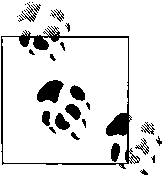
\includegraphics[width=2cm,clip]{paipai.png}
\end{wrapfigure}
\mbox{}该术语来自电气工程领域。水平触发在一个状态发生时触发。边沿触发只有在状态改变的时候才会产生。水平触发在只关心状态时有用。边沿触发则在关心事件本身时有用。
 
\section{存储映射}

除了标准文件I/O,内核提供了另一种I/O方式,允许应用程序将文件映射到内存中,即内存和文件中数据是一一对应的。程序员可以直接通过内存来访问文件,就像操作内存的数据块一样,甚至可以写入内存数据区,然后通过透明的映射机制将文件写入磁盘。

Linux实现了POSIX.1中定义的mmap()系统调用,该调用将对象映射到内存中。本节我们讨论mmap()在I/O中将文件映射到内存的功能;在第八章,我们将看到该调用的其它应用。

\subsection{mmap()}

mmap()调用请求内核将fd表示的文件中从offset处开始的len个字节数据映射到内存中。如果包含了addr,表明优先使用addr为内存中的开始地址。访存权限由prot指定,flags指定了其他的操作行为。

\begin{lstlisting}
  #include <sys/mman.h>
  void * mmap (void *addr, size_t len, int prot, int flags, int fd, off_t offset);
\end{lstlisting}

addr参数告诉内核映射文件的最佳地址。这仅仅是提示,而不是强制,大部分用户传递0。调用返回内存映射区域的开始地址。

prot参数描述了对内存区域所请求的访问权限。如果是PROT\_NONE,此时映射区域无法访问(没有意义),也可以是以下标志位的比特位的或运算值:

\begin{eqlist*}
\item[\textbf{PROT\_READ}] 页面可读。
\item[\textbf{PROT\_WRITE}] 页面可写。
\item[\textbf{PROT\_EXEC}] 页面可执行。
\end{eqlist*}

要求的访存权限不能和打开文件的访问模式冲突。举例来说,如果程序以只读方式打开文件,prot不能设置为PROT\_WRITE。

\begin{center}
\begin{boxedminipage}{\textwidth}
\parindent=2em
\begin{center}\textbf{保护标志,体系结构和安全性}\end{center}

POSIX定义了四种保护位(读,写,执行,避开),一些体系结构只支持其中的子集。其实这很正常,例如对于处理器来讲,读和执行没有区别。这种情况下,处理器可能只有一个读标志。在这些操作系统上,PROT\_READ即代表PROT\_EXEC。不久之前,x86还是这样的系统。

当然,依赖这样的处理方式会导致程序不可移植。可移植的程序在他们需要执行映射中的代码时,会相应的设置PROT\_EXEC。

从另一面来说,这是造成缓冲区溢出攻击盛行的原因之一,即使一个映射不允许执行操作,但处理器仍会执行映射中的代码。

最近x86处理器加入了NX(no-execute)位,它允许可读,但不可执行的映射。在较新的系统上,PROT\_READ不再等同于PROT\_EXEC。
\end{boxedminipage}
\end{center}

flag参数描述了映射的类型和一些行为。其值为以下值按按位或运算的值:

\begin{eqlist*}
\item[\textbf{MAP\_FIXED}] 告诉mmap()把addr看作强制性要求,而不是建议。如果内核无法映射文件到指定地址,调用失败。如果地址和长度指定的内存和已有映射有重叠区域,重叠区的原有内容被丢弃,然后被新内容填充。该选项需要深入了解进程的地址空间,不可移植,所以不鼓励使用。
\item[\textbf{MAP\_PRIVATE}] 映射区不共享。文件映射采用了写时拷贝,进程对内存的任何改变不影响真正的文件或者其它进程的映射。
\item[\textbf{MAP\_SHARED}] 和所有其它映射该文件的进程共享映射内存。对内存的写操作等效于写文件。读该映射区域会受到其他进程的写操作的影响。
\end{eqlist*}

MAP\_SHARED和MAP\_PRIVATE必须指定其中之一,但不能同时指定。更多的标志将在第8章讨论。

当你映射一个文件描述符的时候,描述符引用计数增加。因此,如果你映射文件后关闭文件,你的进程依然可以访问该文件。当你取消映射或者进程终止时,对应的文件引用计数会减 1。

下面的示例代码中以只读方式映射fd所指向的文件,从第一个字节开始,长度为len个字节:

\begin{lstlisting}
  void *p;
  p = mmap (0, len, PROT_READ, MAP_SHARED, fd, 0);
  if (p == MAP_FAILED)
    perror ("mmap");
\end{lstlisting}

图4-1 演示了mmap()的参数对文件与进程地址空间映射的影响。

\begin{figure}[htp]
 \centering
 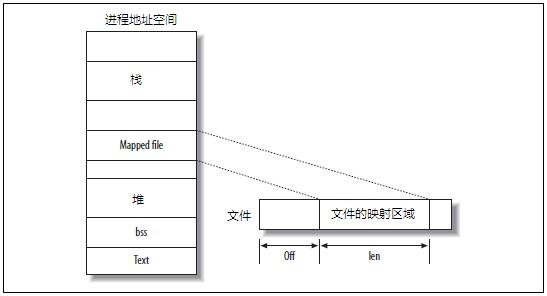
\includegraphics[width=\textwidth]{ch4.jpg}
 \caption{映射文件至进程地址空间}
\end{figure}

\subsubsection{页大小}

\emph{页}是内存中允许具有不同权限和行为的最小单元。因此,页是内存映射的基本块,同时也是进程地址空间的基本块。

mmap()调用操作页。addr和offset参数都必须按页大小对齐。也就是说,它们必须是页大小的整数倍。

所以,映射区域是整数倍个的页。如果len参数不能按页对齐(可能因为需要映射的文件大小不是页大小的整数倍)映射区域延伸到下个空页。多出来的内存,即最后一个有效字节和映射区域边界的区域,用0填充. 该区域的读操作都将返回0。即使使用MAP\_SHARED参数进行映射,写操作也不会影响文件。只有前len个字节需要写回文件。

\textbf{sysconf():}标准POSIX规定的获得页大小方法是通过sysconf(),它将返回一系列系统特定的信息:

\begin{lstlisting}
  #include <unistd.h>
  long sysconf (int name);
\end{lstlisting}

调用sysconf()返回name的值,如果name无效,返回-1。出错时,errno被设置为EINVAL。因为-1对一些情况来讲可能是有效值(例如limits,-1表示没有限制)。明智的做法是在调用前清空errno,并在调用后检查其值。

POSIX定义了\_SC\_PAGESIZE(SC\_PAGE\_SIZE与其同义),大小为一个页面的字节大小。因此,很容易获得页大小:

\begin{lstlisting}
  long page_size = sysconf (_SC_PAGESIZE);
\end{lstlisting}

\textbf{getpagesize():}Linux也提供了getpagesize()函数来获得页大小:

\begin{lstlisting}
  #include <unistd.h>
  int getpagesize (void);
\end{lstlisting}

调用getpagesize()将返回页按字节计数的大小。使用也比sysconf()简单:

\begin{lstlisting}
  int page_size = getpagesize ( );
\end{lstlisting}

并不是所有unix系统支持这个函数,POSIX 1003.1-2001弃用了该函数,在这里包含只是出于完整性考虑。

\textbf{页大小:}页大小由<asm/pages.h>中的宏PAGE\_SIZE定义。因此,第三种获得页大小的方法是:

\begin{lstlisting}
  int page_size= PAGE_SIZE ;
\end{lstlisting}

不同于前两种方法,这种方法是编译时获得页大小,而不是运行时。一些体系结构支持多种机型使用不同页大小,某些机型甚至支持多个不同的页大小。一个二进制文件应该能在给定体系结构下的所有机型上运行,即一次编译,到处运行。硬编码页大小则会终结这种可能性. 因此,你应该在运行时确定页的大小。因为addr和offset通常为0,这种设置并不困难。

此外,未来的内核可能不会将该宏导出到用户空间。我们在此提到它是因为在它在Unix代码中使用很频繁,但是不要在你自己程序中使用它。目前看来,sysconf()是最好的选择。

\subsubsection{返回值和错误码}

调用成功,mmap()返回映射区的地址。失败时,返回MAP\_FAILED,并设置相应的errno。mmap()从不返回0。

可能的errno值:

\begin{eqlist*}
\item[\textbf{EACESS}] 给定的文件描述符不是普通文件,或者打开模式和prot或者flags冲突。
\item[\textbf{EAGAIN}] 文件已被文件锁锁定。
\item[\textbf{EBADF}] 给定文件描述符无效。
\item[\textbf{EINVAL}] addr,len,off中的一个或多个无效。
\item[\textbf{ENFILE}] 打开文件数达到系统上限。
\item[\textbf{ENODEV}] 文件所在的文件系统不支持存储映射。
\item[\textbf{ENOMEM}] 没有足够的内存。
\item[\textbf{EOVERFLOW}] addr + len的结果超过了地址空间大小。
\item[\textbf{EPERM}] 设定了PROT\_EXEC,但是文件系统以不可执行方式挂载。
\end{eqlist*}

\subsubsection{相关信号}

两个和映射区域相关的信号:

\begin{eqlist*}
\item[\textbf{SIGBUS}] 当进程试图访问一块已经无效的映射区域时,该信号产生。比如,文件在映射后被截短。
\item[\textbf{SIGSEGV}] 当进程试图写一块只读的映射区域时,该信号产生。
\end{eqlist*}

\subsection{munmap()}

Linux提供了munmap()来取消mmap()的映射。

\begin{lstlisting}
  #include <sys/mman.h>
  int munmap (void *addr, size_t len);
\end{lstlisting}

munmap()移除进程地址空间从addr开始,len字节长的内存中的所有页面的映射。当映射被解除时,之前关联的内存区域不再有效,如果试图访问将产生SIGSEGV信号。

通常,munmap()的参数是上次mmap()调用的返回值和其参数len。

调用成功返回0;失败返回-1,errno被设置为相应的值。唯一标准的errno值为EINVAL,表明一个或多个参数无效。

作为实例,下面一段代码解除了内存中[addr, addr + len]区间内所有页的映射。

\begin{lstlisting}
  if (munmap (addr, len) == -1)
    perror ("munmap");
\end{lstlisting}

\subsection{存储映射例子}

我们来看一个例子,使用mmap将用户选择的文件输出到标准输出:

\begin{lstlisting}
  #include   <stdio.h>
  #include   <sys/types.h>
  #include   <sys/stat.h>
  #include   <fcntl.h>
  #include   <unistd.h>
  #include   <sys/mman.h>
  int main (int argc, char *argv[])
  {
    struct stat sb;
    off_t len;
    char *p;
    int fd;
    if (argc < 2) {
      fprintf (stderr, "usage: %s <file>\n", argv[0]);
      return 1;
     }
     fd = open (argv[1], O_RDONLY);
     if (fd == -1) {
       perror ("open");
       return 1;
     }
     if (fstat (fd, &sb) == -1) {
       perror ("fstat");
       return 1;           
     }
     if (!S_ISREG (sb.st_mode)) {
       fprintf (stderr, "%s is not a file\n", argv[1]);
       return 1;
     }
     p = mmap (0, sb.st_size, PROT_READ, MAP_SHARED, fd, 0);
     if (p == MAP_FAILED) {
       perror ("mmap");
       return 1;
     }
     if (close (fd) == -1) {
       perror ("close");
       return 1;
     }
     for (len = 0; len < sb.st_size; len++)
       putchar (p[len]);
     if (munmap (p, sb.st_size) == -1) {
       perror ("munmap");
       return 1;
     }
     return 0;
  }
\end{lstlisting}

在本例中,大家唯一不熟悉的系统调用为fstat(),我们将在第七章讲到。在这里,你仅仅需要知道fstat()返回给定文件的信息。S\_ISREG()宏可以检查这些信息,这样我们可以在映射前确保给定文件是个普通文件(相对于设备文件和目录而言)。映射一个非普通文件的行为取决于文件所在设备。一些设备是可以映射的,而有些是不可以的,映射会设置errno为EACCESS。

例子的剩余部分都是很直观的,传递一个文件名作为程序参数。打开文件,确保其为普通文件,映射,关闭,按字节打印文件到标准输出,最后取消映射。

\subsection{mmap()的优点}

相对于read(),write(),使用mmap()处理文件有很多优点。其中包括:

\begin{itemize}
\item 使用read()或write()系统调用需要从用户缓冲区进行数据读写,而使用映射文件进行操作,可以避免多余的数据拷贝。
\item 除了潜在的页错误,读写映射文件不会带来系统调用和上下文切换的开销。就像直接操作内存一样简单。
\item 当多个进程映射同一个对象到内存中,数据在进程间共享。只读和写共享的映射在全体中都是共享的;私有可写的尚未进行写时拷贝的页是共享的。
\item 在映射对象中搜索只需要一般的指针操作。而不必使用lseek()。
\end{itemize}

基于以上理由,mmap()是很多应用的明智选择。

\subsection{mmap()的缺陷}

使用mmap()时需要注意以下几点:

\begin{itemize}
\item 映射区域的大小通常是页大小的整数倍。因此,映射文件大小与页大小的整数倍之间有空间浪费。对于小文件,较大比重的空间被浪费。例如对于4kb的页,一个7字节的映射浪费了4089字节。
\item 存储映射区域必须在进程地址空间内。对于32位的地址空间,大量的大小各异的映射会导致大量的碎片出现,使得很难找到连续的大片空内存。这个问题在64位地址空间明显减少。
\item 创建和维护映射以及相关的内核数据结构有一定的开销。通过上节提到的消除读写时的不必要拷贝的,这些开销可以忽略,对于大文件和频繁访问的文件更是如此。
\end{itemize}

基于以上理由,处理大文件(浪费的空间只占很小的比重),或者在文件大小恰好被page大小整除时(没有空间浪费)优势很明显。

\subsection{调整映射的大小}

Linux提供了mremap()来扩大或减少已有映射的大小。这个函数是Linux特有的:

\begin{lstlisting}
  #define _GNU_SOURCE
  #include <unistd.h>
  #include <sys/mman.h>
  void * mremap (void *addr, size_t old_size, size_t new_size, unsigned long flags);
\end{lstlisting}

mremap()将映射区域[addr, addr + old size)的大小增加或减少到new\_size。依赖进程地址空间的可用大小和flags,内核可以同时移动映射区域。

\begin{wrapfigure}{l}{2.5cm}
  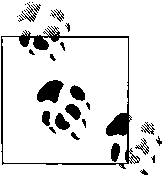
\includegraphics[width=2cm,clip]{paipai.png}
\end{wrapfigure}
\mbox{}[表示区域从低地址开始,包括低地址。)表示区域在高地址为止,不包括高地址,这个惯例称作间隔符号(interval notation)。

flags参数的值可以是0或者MREMAP\_MAYMOVE ,这意味在为了执行调整指定的大小,内核可以根据需求移动映射区域。如果内核可以移动映射,一个较大规模的大小调整操作就可能成功。

\subsubsection{返回值和错误码}

调用成功,mremap()返回指向新映射区域的指针。失败则返回MAP\_FAILED,设置errno为以下值:

\begin{eqlist*}
\item[\textbf{EAGAIN}] 内存区域被锁,不能调整大小。
\item[\textbf{EFAULT}] 给定范围内的一些页不是进程地址空间内的有效页,或者在重新映射给定页时出现问题。
\item[\textbf{EINVAL}] 一个参数无效。
\item[\textbf{ENOMEM}] 给定范围如果不进行移动则无法扩展(MREMAP\_MAYMOVE没有设置),或者进程地址空间内没有足够空闲空间。
\end{eqlist*}

glibc等库经常使用mremap()实现高效的realloc(),可以通过它调整一块由malloc()分配的内存。例如:

\begin{lstlisting}
  void * realloc (void *addr, size_t len)
  {
    size_t old_size = look_up_mapping_size (addr);
    void *p;
    p = mremap (addr, old_size, len, MREMAP_MAYMOVE);
    if (p == MAP_FAILED)
      return NULL;
    return p;
  }
\end{lstlisting}

这段代码只在所有malloc()操作是唯一的匿名映射时有效;即使如此,这段代码也能作为展示尽量提高性能的有用样例。这个例子假设程序员已经写了一个look\_up\_mapping\_size()函数。GNU C library使用mmap()及其相关函数来进行内存分配。我们将在第八章更深入的讨论这个话题。

\subsection{改变映射区域的权限}

POSIX定义了mprotect(),允许程序改变已有内存区域的权限:

\begin{lstlisting}
  #include <sys/mman.h>
  int mprotect (const void *addr, size_t len, int prot);
\end{lstlisting}

调用mprotect()会改变[addr, addr + len)区域内页的访问权限,addr是页对齐的。prot参数和mmap()的prot参数有同样的值:PROT\_NONE,PROT\_READ,PROT\_WRITE,PROT\_EXEC。这些值不是累积的;如果一块区域可读prot值设置了PROT\_WRITE,调用后该区域为只写。

在一些系统上,mprotect()只能操作之前由mmap()创建的区域。在Linux下,mprotect()可以操作任意区域的内存。

\subsubsection{返回值和错误码}

调用成功,mprotect()返回0。失败,返回-1,设置errno值为如下之一:

\begin{eqlist*}
\item[\textbf{EACCESS}] 内存不能设置prot所请求的权限。例如,你试图将一个只读打开的文件的映射设置为可写。
\item[\textbf{EINVAL}] addr无效或者没有页对齐。
\item[\textbf{ENOMEM}] 内核没有足够空间满足请求,或者请求区域内有页面不是进程地址空间内的有效部分。
\end{eqlist*}

\subsection{使用映射机制同步文件}

POSIX提供了一个使用存储映射机制并与fsync()等价的系统调用:

\begin{lstlisting}
  #include <sys/mman.h>
  int msync (void *addr, size_t len, int flags);
\end{lstlisting}

调用msync()可以将mmap()生成的映射在内存中的任何修改回写到磁盘,达到同步内存中的映射和被映射的文件的目的。具体来说,文件或者文件子集在内存中的映射从addr开始的len长度字节被写回到磁盘。addr参数必须是页对齐的,通常是上次mmap()调用的返回值。

不调用 msync(),无法保证在映射取消前,修改过的映射会被写回到硬盘。这一点与write()有所不同,被write()修改的缓冲区被保存在一个队列中等待被写回。当写入内存映射时,进程直接修改内核页缓存中的文件页,而无需经过内核。内核不会立刻同步页缓存到硬盘。

flag 参数控制同步操作的行为。它的值为以下值的按位或操作:

\begin{eqlist*}
\item[\textbf{MS\_ASYNC}] 指定同步操作异步发生。更新操作由系统调度,msync()会立即返回,不用等待write()操作完成。
\item[\textbf{MS\_INVALIDATE}] 指定该块映射的其它所有拷贝都将失效。未来对该文件任意映射的操作将直接同步到磁盘。
\item[\textbf{MS\_SYNC}] 指定同步操作必须同步进行。msync() 直到所有页写回磁盘后返回。
\end{eqlist*}

MS\_ASYNC和MS\_SYNC必须指定其一,二者不能共用。

用法很简单:

\begin{lstlisting}
  if (msync (addr, len, MS_ASYNC) == -1)
    perror ("msync");
\end{lstlisting}

这个例子是异步的将文件的映射区域[addr, addr+len)同步到磁盘。

\subsubsection{返回值和错误码}

调用成功,msync()返回0。失败,调用返回-1,设置errno为相应值。以下为errno的有效值:

\begin{eqlist*}
\item[\textbf{EINVAL}] flags 参数同时设置了MS\_SYNC和MS\_ASYNC,设置了除以上三个合法参数外的其他参数,或者没有页对齐。
\item[\textbf{ENOMEM}] 指定的内存区域(或其中一部分)没有被映射。注意按POSIX规定,Linux在请求同步一块部分解除映射的内存时,将返回ENOMEM,但是这样可能同步一些无效的区域。
\end{eqlist*}

在2.4.29版本的内核之前,msync()返回EFAULT,而不是ENOMEM。

\subsection{映射提示}

Linux提供了madvise()系统调用,可以让进程在如何访问映射区域上给内核一定的提示。内核会据此优化自己的行为,尽量更好的利用映射区域。内核一般会动态调整自己的行为,通常即便在没有明确提示时也能保证较好的性能,但是适当的提示信息可以确保在一定负载下获得所需的缓存和执行正确的预读。

调用会指示内核该如何对起始地址为addr,长度为len的内存映射区域进行操作。

\begin{lstlisting}
  #include <sys/mman.h>
  int madvise (void *addr, size_t len, int advice);
\end{lstlisting}

如果len为0,内核将对所有起始地址为addr的映射使用该提示信息。参数advice可以是下列之一:

\begin{eqlist*}
\item[\textbf{MADV\_NORMAL}] 对给定的内存区域,应用程序没有特殊提示,按正常方式操作。
\item[\textbf{MADV\_RANDOM}] 应用程序将以随机顺序访问指定范围的页。
\item[\textbf{MADV\_SEQUENTIAL}] 应用程序意图从低地址到高地址顺序访问指定范围的页。
\item[\textbf{MADV\_WILLNEED}] 应用程序将很快访问指定范围的页。
\item[\textbf{MADV\_DONTNEED}] 应用程序短期内不会访问指定范围内的页。
\end{eqlist*}

内核得到提示后真正采取的行为是与具体的实现相关的:POSIX仅仅指定了提示的含义,而没有规定具体的行为。2.6内核以如下方式进行处理:

\begin{eqlist*}
\item[\textbf{MADV\_NORMAL}] 内核行为照常,进行一定程度的预读。 
\item[\textbf{MADV\_RANDOM}] 内核不做预读,每次物理读操作只读取最小量的数据。
\item[\textbf{MADV\_SEQUENTIAL}] 内核大量预读。
\item[\textbf{MADV\_WILLNEED}] 内核将给定的页预读至内存。
\item[\textbf{MADV\_DONTNEED}] 内核释放所有和给定页相关的资源,丢弃所有被修改的,未同步写回的页。后续对映射数据访问会使数据重新载入内存。
\end{eqlist*}

典型用法如下:

\begin{lstlisting}
  int ret;
  ret = madvise (addr, len, MADV_SEQUENTIAL);
  if (ret < 0)
    perror ("madvise");
\end{lstlisting}

该调用告诉内核,进程意图连续访问内存区域[addr, addr + len)。

\begin{center}
\begin{boxedminipage}{\textwidth}
\parindent=2em
\begin{center}\textbf{预读}\end{center}

当Linux内核访问磁盘上的文件时,通常会采用众所周知的预读(readahead)来优化自己的操作。也就是说,当文件的某块内容被加载时,内核也会读取这块内容之后的块。如果随后有对该块的访问请求(例如连续访问某个文件时)内核可以马上返回数据。因为磁盘有缓冲区(磁盘自己也会有预读行为),而且文件通常是连续分布在磁盘的,这个优化的开销是很低的。

预读通常是有好处的,但是具体的优化效果依赖于预读的程度。很大的预读窗口在连续访问文件时很有效,而对随机访问来讲,预读则是无用的开销。

正如我们在第二章的“内核内幕”一节所讨论的,内核会动态的调整预读窗口,以保证在预读窗口中一定的命中率。高命中率则意味着最好使用再大一点的预读窗口,反之则提示使用小一点的预读窗口。应用程序可以通过madvise()系统调用来影响预读窗口的大小。
\end{boxedminipage}
\end{center}

\subsubsection{返回值和错误码}

调用成功,madvise()返回0,失败时,返回-1,设置errno为相应值。以下为有效错误值:

\begin{eqlist*}
\item[\textbf{EAGAIN}] 内核内部资源(可能是内存)不可用,进程可以重试。
\item[\textbf{EBADF}] 区域存在,但是没有映射到文件。
\item[\textbf{EINVAL}] 参数len是负的,addr不是页对齐的,advice参数无效,或者页面被锁,或以MADV\_DONTNEED方式共享该区域.
\item[\textbf{EIO}] 使用MADV\_WILLNEED操作时引起的内部I/O错误。
\item[\textbf{ENOMEM}] 给定的区域不是进程地址空间的有效映射,或者设置MADV\_WILLNEED,但是没有足够内存可供分配。
\end{eqlist*}

\section{普通文件I/O提示}

上一小节,我们学习了如何给内核提供存储映射的操作提示。在本节,我们将学习在普通文件I/O 时,如何给内核提供操作提示。Linux提供了两个满足要求的函数:posix\_fadvise()和readahead()。

\subsection{posix\_fadvise()}

正如它的名字一样,该函数由POSIX 1003.1-2003定义:

\begin{lstlisting}
  #include <fcntl.h>
  int posix_fadvise (int fd, off_t offset, off_t len, int advice);
\end{lstlisting}

调用posix\_fadvise()会给出内核在文件fd的[offset, offset + len) 范围内操作提示。如果len为0,则该提示作用于区间[offset, length of file]。一般用法是设置len和offset为0,从而使设置应用到整个文件。

advice 的可用选项和madvise()类似。准确的讲,是以下选项的其中之一:

\begin{eqlist*}
\item[\textbf{POSIXFADV\_NORMAL}] 应用程序在给定文件的给定区域没有特殊要求,按正常情况处理。
\item[\textbf{POSIX\_FADV\_RANDOM}] 应用程序在给定范围内趋向于随机访问。
\item[\textbf{POSIX\_FADV\_SEQUENTIAL}] 应用程序在给定范围内趋向于从低地址到高地址顺序访问。
\item[\textbf{POSIX\_FADV\_WILLNEED}] 应用程序可能在最近访问指定范围。
\item[\textbf{POSIX\_FADV\_NOREUSE}] 应用程序可能在最近访问给定范围,但只访问一次。
\item[\textbf{POSIX\_FADV\_DONTNEED}] 应用程序最近可能不会访问给定范围。
\end{eqlist*}

和madvise()一样,内核对这些提示的处理因不同的实现而有所区别,甚至不同版本的Linux内核的处理方式也不尽相同。下面是目前内核的处理方式:

\begin{eqlist*}
\item[\textbf{POSIX\_FADV\_NORMAL}] 内核行为如常,有适量的预读行为。
\item[\textbf{POSIX\_FADV\_RANDOM}] 内核禁止预读,每次物理读操作尽可能的读取最少量的数据。
\item[\textbf{POSIX\_FADV\_SEQUENTIAL}] 内核大量预读,读取预读窗口两倍长度的数据。
\item[\textbf{POSIX\_FADV\_WILLNEED}] 内核开始预读,并将指定页读到内存中。
\item[\textbf{POSIX\_FADV\_NOREUSE}] 当前,其行为与POSIX\_FADV\_WILLNEED一致;未来内核可能会将其做为''使用一次''的一种附加优化。在madvise中没有与之对应的选项。
\item[\textbf{POSIX\_FADV\_DONTNEED}] 内核丢弃所有缓存的数据。与其他选项不同,它与madvise()中对应选项行为不一样。
\end{eqlist*}

以下代码片段要求内核随机、无序的访问 fd 代表的文件:

\begin{lstlisting}
  int ret;
  ret = posix_fadvise (fd, 0, 0, POSIX_FADV_RANDOM);
  if (ret == -1)
    perror ("posix_fadvise");
\end{lstlisting}

\subsubsection{返回值和错误码}

调用成功返回0,失败返回-1,设置 errno 为下列值之一:

\begin{eqlist*}
\item[\textbf{EBADF}] 文件描述符无效。
\item [\textbf{EINVAL}] advice无效,文件描述符指向一个管道,或者设定选项无法应用到给定的文件。
\end{eqlist*}

\subsection{readahead()系统调用}

posix\_fadvise()是2.6内核中新加入的系统调用。在此之前,readahead()可以完成posix\_fadvise()使用POSIX\_FADV\_WILLNEED选项时同样的功能。但不同于posix\_fadvise()的是,readahead()是Linux所独有的:

\begin{lstlisting}
  #include <fcntl.h>
  ssize_t readahead (int fd, off64_t offset, size_t count);
\end{lstlisting}

readahead()调用将读入fd表示文件的[offset, offset + count)区域到页缓存中。

\subsubsection{返回值和错误码}

调用成功返回 0,失败返回-1,设置errno为下列值之一:

\begin{eqlist*}
\item[\textbf{EBADF}] 文件描述符无效
\item[\textbf{EINVAL}] 文件描述符对应的文件不支持预读。
\end{eqlist*}

\subsection{“经济实用“的操作提示}

通过向内核传递一些操作提示,一些普通应用的效率可以获得提升。这些信息对于减轻繁重的I/O负担很有助益。由于磁盘速度与现代处理器速度的不匹配,有益的提示甚至很少的数据位上的提升都是很有帮助的。

在读取一个文件的大部分内容时,进程可以通过设置POSIX\_FADV\_WILLNEED 要求内核把文件预读到页缓存中。 I/O 操作将在后台异步进行。当应用最终要访问文件时,访问操作可以立即返回,不会被阻塞。

相反的,在读取或写入大量数据后(比如硬盘上连续的视 频数据流),进程可以设置POSIX\_FADV\_DONTNEED要求内核丢弃缓存中的内容。大量的流操作会填满页缓冲区。如果进程不会再次访问这些数据,则意味着页缓冲区中充斥了过量的数据,其代价是导致没有空间保存有用的数据。因此对于视频流一类的应用,需要定期的请求将数据从缓存中清除。

一个进程试图读取整个文件时,设置POSIX\_FADV\_SEQUENTIAL 要求内核大量预读。相反的,如果一个进程知道自己将随机访问文件,设置POSIX\_FADV\_RANDOM,告诉内核预读没有用,只会带来无谓的开销。

\section{同步(Synchronized),同步(Synchronous)及异步( Asynchronous)操作}

\textbf{译者注:由于synchronized与synchronous一半都翻译为同步,在本节中,我们对每一个翻译为同步的词都会增加相关的英文原文。}

Unix 操作系统在使用术语同步(synchronized),非同步(nonsynchronized),同步(synchronous),异步(asynchronous)时很随意,完全忽视了这几个词所引起的困惑(在英语中,synchronized和synchronous之间的区别很小)。

同步(synchronous)写操作在数据全写到内核缓冲区之前是不会返回的。同步(synchronous)读操作在数据写到应用程序在用户空间的缓冲区之前是不会返回的。相反的,异步(asynchronous)写操作在用户空间还有数据时可能就返回了;异步(asynchronous)读操作在数据准备好之前可能就返回了。也就是说,操作不会被放入操作队列中以便在稍后进行。当然,在这种情况下必须有一定的机制来确认操作是否完成以及完成的程度。

一个同步的(synchronized)操作要比同步(synchronous)操作的限制更多,也更安全。同步的(synchronized)写操作把数据写回硬盘,确保硬盘上的数据和内核缓冲区中的是同步的。同步(synchronized)的读操作总是返回最新的数据(有可能从硬盘中读取)。

总的来说,同步(synchronous)和异步(asynchronous)指I/O操作在返回前是否等待某些事件(如数据的存储)返回。而术语同步(synchronized)和异步(asynchronized)准确地指定了某个事件必须发生(例如把数据写回硬盘)。

通常,Unix的写操作是同步(synchronous)和非同步的(nonsynchronized);读操作是同步(synchronous)和同步的(synchronized)。\footnote[1]{从技术角度看,读操作和写操作类似,是非异步的(nonsynchronized),但是内核页缓冲中包含最新的数据。也就是说,页缓冲中的数据一般都比磁盘上的数据要新一些。在这种情况下,实际上的操作经常是同步的。采用别的方式,也没有太多争议。}对于写操作,上述特性的任意组合都是可能的,如表4-1所示。

\begin{table}[htp]
\caption{\emph{写操作的同步性}}
\begin{tabular}{p{2.5cm}p{5.5cm}p{5.5cm}}\toprule
\rowcolor[gray]{.9}
 & \textbf{Synchronized} & \textbf{Nonsynchronized} \\ \midrule
\textbf{Synchronous} & 写操作直到数据写入磁盘后才返回。当打开文件时使用O\_SYNC参数是才按照这种方式执行。 & 写操作在数据保存入内核缓冲区后返回。这是通常的行为。 \\
\textbf{Asynchronous} & 写操作在请求被加入队列后返回。一旦该操作被执行,会确保数据写入磁盘。 & 写操作在请求被加入队列后返回。一旦该操作被执行,会确保数据写入内核缓冲区。\\ \bottomrule
\end{tabular}
\end{table}

因为读取旧数据没有意义,读操作通常是同步的(synchronized)。这样的操作既可以是同步(synchronous)的,也可以是异步(asynchronous)的,如表4-2所示。

\begin{table}[htp]
\caption{\emph{读操作的同步性}}
\begin{tabular}{p{2.5cm}p{11.5cm}}\toprule
\rowcolor[gray]{.9}
 & \textbf{Synchronized} \\ \midrule
 \textbf{Synchronous} & 读操作直到最新数据保存到提供的缓冲区后才返回。(这是通常的行为。) \\
 \textbf{Asynchronous} & 读操作在请求被加入队列后返回。一旦该操作被执行,返回最新数据。 \\ \bottomrule
\end{tabular}
\end{table}

在第二章,我们讨论和如何使写操作进行同步(synchronized)(设置O\_SYNC标志),如何确保所有I/O操作是同步的(synchronized)(通过 fsync()和friends)。现在我们来看看如何使读写(asynchronous)异步完成。

\subsection{异步I/O}

执行异步(asynchronous)I/O需要内核在底层的支持。 POSIX 1003.1-2003定义了aio接口,幸运的是Linux实现了aio。aio库提供了一系列函数来实现异步I/O提交以及在完成时收到通知。

\begin{lstlisting}
  #include <aio.h>
  /* asynchronous I/O control block */
  struct aiocb {
    int aio_filedes;               /* file descriptor */
    int aio_lio_opcode;            /* operation to perform */
    int aio_reqprio;               /* request priority offset */
    volatile void *aio_buf;        /* pointer to buffer */
    size_t aio_nbytes;             /* length of operation */
    struct sigevent aio_sigevent;  /* signal number and value */
    /* internal, private members follow... */
  };
  int aio_read (struct aiocb *aiocbp);
  int aio_write (struct aiocb *aiocbp);
  int aio_error (const struct aiocb *aiocbp);
  int aio_return (struct aiocb *aiocbp);
  int aio_cancel (int fd, struct aiocb *aiocbp);
  int aio_fsync (int op, struct aiocb *aiocbp);
  int aio_suspend (const struct aiocb * const cblist[], int n, const struct timespec *timeout);   
\end{lstlisting}

\subsubsection{基于线程的异步I/O}

Linux只支持使用O\_DIRECT标志打开的文件上的aio。要想在没有设置O\_DIRECT标志的普通文件上使用aio,我们必须自己来实现。没有内核的支持,我们只能希望近似实现异步I/O,在实际应用中达到相似的效果。

第一,我们将看到为什么应用程序的开发者需要异步I/O:

\begin{itemize}
\item 实现非阻塞I/O
\item 为了分离内核的I/O排队,I/O请求提交,在操作完成时收到通知。
\end{itemize}

第一点是基于性能的考虑。如果I/O操作永远不会阻塞,就不会出现I/O超负荷的情况,进程也不必被I/O所束缚。第二点是基于过程的考虑,只是另一种处理I/O的方式。

达到这些目的最常用的方式是线程(调度将在第五六章讲到)。这种方法需要完成下列任务:

\begin{enumerate}
\item 创建一个线程池来处理所有的I/O。
\item 实现将I/O操作加入工作队列的一系列函数。
\item 使这些函数返回唯一的I/O描述符,来区分相关的I/O操作。每个工作线程响应队列首的I/O请求,提交到内核,等待它们完成。
\item 完成后,把操作的结果(返回值,错误码,所有读取的数据)加入到一个结果队列中。
\item 实现一系列从结果队列中获取状态信息的函数,使用最初返回的I/O描述符区分每个操作。
\end{enumerate}

这和POSIX的aio的相关函数的行为很近,但是由此也增加了线程管理的开销。

\section{I/O调度器和I/O性能}

在现代系统中,硬盘和系统其它部分的性能差距很大,而且还在增大。硬盘性能最糟糕的部分是执行seek操作的时候,在此过程中磁头从磁盘的一个部分移动到另一个部分。当大多数操作都以处理器周期(大概是1/3纳秒)来衡量的时候,一次单独的seek操作平均需要8毫秒的时间,尽管这看起来并不长,但却是cpu周期的2500万倍。

当了解了硬盘和系统其它部分的性能差距,我们会发现等待 I/O 操作按它们请求顺序完成将是非常原始和低效的。因此,现代操作系统内核都实现了I/O调度器,通过管理I/O请求的顺序和次数使磁盘寻道次数和移动距离最小化。I/O调度器尽力将硬盘访问的性能损失控制在最小。

\subsection{磁盘寻址}

要理解I/O调度器的工作机制,需要先了解一些背景知识。硬盘基于用柱面(cylinders),磁头(heads),和扇区(section)几何寻址方式来获取数据,这种方式也被成为CHS寻址。每个硬盘都是由多个盘片组成,每个盘片包括一个磁盘、一个主轴和一个读写头。你可以把每个盘片看作一个CD,硬盘上所有盘片看作一摞CD。每个盘片分成很多环状的磁道,就像CD上一样。每个磁道分为整数倍个扇区。

要确定某块特定数据单元在硬盘上的位置,驱动程序需要知道三个值:柱面,磁头和扇区。柱面值确定了数据在哪个磁道上。如果把盘片放成一摞,磁道在所有盘片上确定了一个柱面。换句话说,一个柱面代表了所有盘片上离盘中心相同距离的磁道。磁头值表明了准确的磁头(即准确的盘片)。现在搜索定位到了单个盘片上的单个磁道。磁盘驱动然后利用扇区找到磁道上准确的扇区。搜索结束:硬盘驱动知道在哪个盘片,哪个磁道,哪个扇区查找数据。然后定位读写头到正确的盘片上正确的磁道,从正确的扇区读写。
     
幸运的是,现代系统不会直接操作硬盘的柱面、磁头和扇区。硬盘驱动将每个柱面/磁头/扇区的三元组映射到唯一的块号(也叫物理块或设备块),——更准确的说,映射到指定的扇区。现代操作系统可以直接使用块号(即逻辑块寻址(LBA))访问硬盘,硬盘驱动程序转换块号到正确的CHS地址\footnote[1]{在块绝对数量上限制很大程度上导致了近年来在磁盘容量上的各种限制}。很自然的,块到CHS的映射是连续的:物理块n和逻辑块n + 1是物理上相邻的。稍后我们将看到,这种连续的映射是很重要的。

文件系统存在于软件层。它们操作自己的操作单元,即逻辑块(有时候称作文件系统块,或者块)。逻辑块的大小必须是物理块大小的整数倍。换句话说,文件系统的逻辑块映射到一个或多个硬盘物理块。

\subsection{调度器的功能}

I/O调度器实现两个基本操作:合并(merging)和排序(sorting)。合并(merging)操作是将两个或多个相邻的I/O请求的过程合并为一个。考虑两次请求,一次读取5号块,另一次读取6和7上的数据。这些请求被合并为一个对块5到7的操作。总的I/O吞吐量可能一样,但是I/O的次数减少了一半。
     
排序(sorting)是选取两个操作中相对更重要的一个,并按块号递增的顺序重新安排等待的I/O请求。比如说,I/O操作要求访问块52,109,和7,I/O调度这三个请求以7,52,109的顺序进行排序.如果一个请求现在要访问81,它将被插入到访问52和109的中间。I/O调度器然后按他们在队列中的顺序一次调度:7,然后52,然后81,最后109。

按这种方式,硬盘头的移动距离最小。不用无计划的移动(在整个磁盘中来回无序的移动进行查找),磁头以平滑、线性的方式移动。因为寻址是I/O操作中代价最高的部分,改进该操作可以使I/O性能获得提升。

\subsection{改进读请求}

每次读请求必须返回最新的数据。因此,当请求的数据不在页缓存中时,读请求在数据从磁盘读出前一直会阻塞——这可能是一个相当漫长的操作。我们将这种性能损失称为读延迟(read latency)。

一个典型的程序可能在短时期有几个 I/O 请求。因为每个请求都分别进行同步,稍后的请求将依赖于前面请求。比如说,我们要读取一个目录下所有的文件。应用程序打开第一个文件,读取一块,等待数据,然后读下一段数据,如此往复,直到整个文件被读取。然后进程开始读取下一个文件。所有的请求都是串行进行的:直到当前请求结束,后续请求才可以执行。

这和写请求(缺省是非同步的)形成了鲜明的对比,写请求在短时间内不需要发起任何I/O操作。从用户空间程序角度看,写操作不受硬盘性能的影响。写操作只有在和读操作组合使用的时候才会引起问题:因为写操作的数据流,它们可以吸引内核和硬盘的注意力。这种现象就是著名的writes-starving-reads问题。

如果I/O调度器以插入的顺序来对请求排序,可能会无限期的推迟对较远块的访问请求。继续看一下我们的前一个例子。如果新的请求不断加入,比如都是50-60间的,第109 块的访问请求将不会被调度到。因为读延迟的问题很严重,可能会极大得影响系统性能。所以 I/O 调度器使用一种机制避免''饿死''的发生。

最简单的方法就是像2.4内核那样采用Linux电梯调度法\footnote[1]{Linus以他自己的名字命名了这个调度器。这种算法因为和解决电梯平滑运行的问题类似,所以也称为电梯算法。},在该方法中,如果队列中有一定数量的旧的请求,则停止插入新的请求。这样整体上可以做到平等对待每个请求,但在读的时候,却增加了读延迟 (read latency)。问题在于这种检测方法太简单。意识到这点,2.6内核丢弃了Linus电梯调度算法,转而使用了几种新的调度器算法。

\subsubsection{Deadline I/O调度器}

Deadline I/O调度器是为了解决2.4调度程序及传统的电梯调度算法的问题。Linus电梯算法维护了一个经过排序的I/O等待列表。队列首的I/O请求是下一个被调度的。Deadline I/O 调度器保留了这个队列,为了进一步改进了原来的调度器,增加了两个新的队列:读FIFO队列和写FIFO 队列。队列中的项按请求提交时间排序。读 FIFO 队列,如它名字所述,只包含读请求,同样写FIFO队列只包含写请求。FIFO队列中的每个请求都设置一个过期时间。读FIFO队列的过期时间设置为500毫秒。写队列则为5秒。

当一个新的I/O请求提交后,它被按序插入到标准队列,然后加入到相应队列(读或写)的队尾。通常情况下,硬盘总是先发送标准队列头的I/O请求。因为普通队列是按块号排列的 (linus电梯调度法也如此),这样可以通过减小查找次数来增大全局吞吐量。

当一个FIFO队列头的请求超出了所在队列的过期时间时,I/O调度器停止从标准I/O队列中调度请求,转而调度这个FIFO队列的队首请求。I/O调度程序只需检查处理队首的请求,因为它是队列中等待时间最久的。

按这种方式,Deadline I/O调度器在I/O请求上加入了最后期限。虽然不能保证在过期时间前调度I/O请求,但是一般都是在过期时间左右调度请求。因此,Deadline I/O调度器能提供很好的吞吐量,而不会让任一个请求等待过长的时间。因为读请求被赋予更小的过期时间,writes-starving-reads问题的发生次数降到了最低。

\subsubsection{Anticipatory I/O调度器}

Deadline I/O调度器表现很好,但是并不完美。回忆一下我们关于读依赖的讨论。使用 Deadline I/O调度器时,在一系列读请求中的第一个,在它的截止时间前或马上到来时将会很快被响应,然后I/O调度程序返回,处理队列中其它I/O请求。到现在为止,暂时没什么问题。但是假设应用突然提交一个读请求,而且它的即将到截止时间,I/O调度器响应该请求,在硬盘查找请求的数据,然后返回,再处理队列中其它请求。这样的前后查找可能持续很长事件,在很多应用中都能看到这样的情况。当延迟保持在很小时,因为要不断的处理读请求并在磁盘上查找数据,所以总的吞吐量并不是很好。如果硬盘能够停下来等待下一个读请求,而不处理排序队列中的请求,性能将会得到一定的提升。不幸的是,在下次应用程序被调度并提交下一个独立的读请求器,I/O调度器已经移动磁头了。
     
当面对众多独立的读请求时,问题依然会出现--每个读请求在前一个请求返回后才会执行,当应用程序得到数据,准备运行并提交了下一个读请求时,I/O调度程序已经去处理其他的请求了。这样导致了每次搜索时都要进行不必要的寻道操作:查找数据,读数据,返回。如果存在一种方法使I/O调度器预知对磁盘同一部分的访问,将在下一个请求中提交,就可以等待下次的读,而不必往复进行查找定位。花几毫秒的等待时间来避免可怕的查找,是很值得的。
     
anticipatory I/O调度器的工作原理是很清楚的。它像Deadlne一样开始,但是它具有预测机制。当一个读操作被提交,anticipatory I/O调度器在它的终止期限前调度它。不同于Deadline I/O调度器的是,anticipatory I/O调度器会等待6毫秒。如果应用程序在6毫秒内对硬盘同一部分发出另一次读请求,读请求立刻被响应,anticipatory I/O调度器继续等待。如果6毫秒内没有收到读请求,anticipatory I/O调度器确认预测错误,然后返回进行正常操作(例如处理标准队列中的请求)。如果适当数目的请求预测正确,则可以节省大量的时间(为了节省寻道时间,值得每次都做这样的处理)。因为大部分读是相互依赖的,预测节省了大量时间。

\subsubsection{CFQ I/O调度器}

尽管在方法上有所区别,但Complete Fair Queuing(CFQ)I/O调度器和上述调度程序的目标是相同的。\footnote[1]{下面的文字讨论目前实现的CFQ I/O调度器。之前的经典原型没有使用时间片或启发式预测,但是以类似的方式工作。}使用CFQ时,每个进程都有自己的队列,每个队列分配一个时间片。 I/O 调度程序使用轮转方式访问并处理队列中的请求,直到队列的时间片耗尽或所有的请求都被处理完。后一种情况,CFQ I/O调度器将会空转一段时间(默认10毫秒),等待当前队列中新的请求。如果预测成功,I/O调度器避免了查找操作。如果预测无效,调度程序转而处理下一个进程的队列。

在每个进程的队列中,同步(synchronized )的请求(例如读操作)被赋予比非同步请求更高的优先级。按在这种情况下,CFQ更希望进行读操作,也避免了writes-starving-reads问题。因为进程队列设置,CFQ调度器对所有进程都是公平的,同时还提供了优秀的全局性能。

CFQ 调度器适合高负载的情况,并且是这种情况下的第一选择。

\subsubsection{Noop I/O调度器}

Noop I/O调度程序是目前最简单的调度器。无论什么情况,它都不进行排序操作,只是简单的合并。它一般用在不需要对请求排队的特殊设备上。

\subsection{选择和配置你的I/O调度器}

默认的I/O调度器可以在启动时可以通过内核参数iosched来指定。有效的选项有as,cfq,deadline,和 noop。也可以在运行时针对每个块设备进行选择,可以通过修改/sys/block/device/queue/scheduler来完成。读这个文件可以知道当前的I/O调度器是什么,把上述有效选项写入这个文件可以更改I/O调度程序。例如,要设置设备hda的I/O调度程序为CFQ,可以使用如下方式:

\begin{verbatim}
  #echo cfq >/sys/block/hda/queue/scheduler
 \end{verbatim}

目录/sys/block/device/queue/iosched包含了管理员可以获得和设置的I/O调度器相关的选项。选项依赖于当前I/O调度器。改变任何设置都需要root权限。

一个好的程序员写的程序不会涉及到底层的I/O 子系统。但是,对其的了解毫无疑问有助于写出更好的代码。

\subsection{优化I/O性能}

因为磁盘I/O相比系统其它部分很慢,同时I/O系统又是现代计算机很重要的一个部分,因此使I/O性能达到最优是非常重要的。

减少I/O操作的次数(通过将很多小的操作聚集为一些大的操作),实现块对齐的I/O,或者使用用户空间缓冲(见第三章),利用高级I/O的优点,如向量I/O,定位I/O(见第二章)和异步I/O,都是系统编程过程中需要经常考虑的重要步骤。

一些关键任务和I/O操作频繁的应用程序,可以使用额外的技巧来优化性能。如同前面讨论的,即使Linux内核也利用高级I/O调度器减少磁盘寻道次数,用户空间的程序可以使用类似方式,实现更多的性能提升。

\subsubsection{用户空间I/O调度}

进行大量I/O调用的I/O密集型的应用可以通过使用类似于Linux I/O调度器的方法,来对挂起的I/O请求进行排序和合并,进而获得更多的性能提升。\footnote[1]{只能将这种技术应用于I/O操作频繁的应用或者关键应用上。I/O请求很少的程序(假设没有什么需要排序的)则没必要对I/O操作进行排序。}

既然你已经知道I/O调度器将按块排序请求,减少寻道,并尽量将磁头以线性平滑的方式移动,为什么还要在应用程序中重复一次呢? 假设有一个应用,提交大量未排序的I/O请求。这些请求以随机顺序进入I/O调度器的队列。I/O调度器在向硬盘转发请求前对其进行排序和合并,但是当请求开始向磁盘提交时,应用程序仍在不断提交I/O请求。I/O调度程序只能排序大量请求中的一小部分,其余的都被挂起。虽然每一部分请求都被排序,但是从整个队列和未来的可能会产生的请求的角度来看,这些都不在其中。

因此,如果一个应用程序会产生大量请求,尤其是请求可能是遍布整个磁盘的数据,最好在提交之前对其排序,确保它们有序提交给I/O 调度器,这样将带来很大的性能提升。
     
对于同样的信息,用户空间的程序和内核不见得有同样的访问权限。在 I/O调度器的最底层,请求已经是以物理块的形式进行组织。对物理块进行排序是很简单的。但是,在用户空间,请求是以文件和文件偏移的形式存在的。用户应用程序必须获取信息,并文件系统的布局做适当的猜测。
     
为了使I/O请求能以有利于寻址操作的顺序提交,用户空间程序可以做不同的处理。它们可按照以下方式进行排序:

\begin{enumerate}
\item 完整路径
\item inode编号
\item 文件的物理块
\end{enumerate}

每个选项都做了一定程度上的折衷。让我们分别来讨论一下各种情况。

\textbf{按路径排序。}这是最简单的,也是效率最低的接近块排序的方法。在大部分文件系统采用的布局算法中,每个目录里的文件,(包括拥有共同父目录的两个子目录)倾向于在磁盘上相邻分布。同一个目录中的文件,如果在间隔很短的时间内依次创建,相邻的几率更大。
  
按路径排序,粗略接近文件在磁盘上的物理位置分布。在同一个目录下的文件显然比在文件系统完全不同两部分的两个文件有更大的概率邻近分布。这种方法缺点是没有考虑文件系统的碎片,如果文件系统碎片很多,按路径排序的作用越小。即使忽略了碎片,按路径排序也只能说是接近实际的物理块顺序。好的一面是,路径排序至少对于所有文件系统都是可用的。不考虑在文件布局上的接近程度,空间局部性显示使用路径排序至少具有中等精确度。此外,这种排序方法很容易实现。

\textbf{按inode排序。}inode是Unix中包含和文件唯一相关的元信息的结构。一个文件可能占用多个物理块,但只有一个inode,其中包含了文件大小,权限,所有者等信息。我们将在第 7 章更深入的讨论 inode。现在,你只需要知道两点:每个文件都有一个inode与之关联,这个inode是由数字来唯一标识。

使用inode排序比路径排序更有效,考虑如下关系:

\begin{verbatim}
  文件i的inode序号 < 文件j的inode序号
\end{verbatim}

通常情况下意味着:

\begin{verbatim}
  文件i的物理块 < 文件j的物理块
\end{verbatim}

对Unix的文件系统(如ext2和ext3)来讲,这是毫无疑问的。对没有使用真实节点的文件系统,任何事情都是可能的,但是inode号(不管它映射到哪)都是一个好的近似选择。对于实际上不使用inode的文件系统来讲,存在各种可能性。但是使用inode(无论其如何映射)排序也不失为一种比较好的方法。

我们可以通过stat()系统调用来获得inode序号,更具体的方法我们将在第七章讨论。获取每个参与I/O请求的文件的inode序号,然后以inode序号的升序方式对每个请求进行排序。

以下示例程序可以输出给定文件的inode编号:

\begin{lstlisting}
  #include  <stdio.h>
  #include  <stdlib.h>
  #include  <fcntl.h>
  #include  <sys/types.h>
  #include  <sys/stat.h>
  /*
   * get_inode - returns the inode of the file associated
   * with the given file descriptor, or -1 on failure
   */
  int get_inode (int fd)
  {
    struct stat buf;
    int ret;
    ret = fstat (fd, &buf);
    if (ret < 0) {
      perror ("fstat");
      return -1;
    }
    return buf.st_ino;
  }
  int main (int argc, char *argv[])
  {
    int fd, inode;
    if (argc < 2) {
      fprintf (stderr, "usage: %s <file>\n", argv[0]);
      return 1;
     }
     fd = open (argv[1], O_RDONLY);
     if (fd < 0) {
       perror ("open");
       return 1;
     }
     inode = get_inode (fd);
     printf ("%d\n", inode);
     return 0;
  }
 \end{lstlisting}

get\_inode()函数可以很容易的在你的程序中使用。

按inode编号排序有如下优点: inode编号容易获取,容易排序,和文件的物理布局很接近。主要的缺点是碎片会降低接近的程度,接近程度只是估算,在非Unix系统上也不够准确。无论如何,使用inode进行排序都是在用户空间I/O请求调度中最常用的方法。

\textbf{按物理块排序。}使用物理块进行排序,最好的方法是设计你自己的电梯算法。如之前讨论的,逻辑块是文件系统最小的分配单元,每个文件被分割成若干逻辑块。逻辑块的大小和文件系统有关;每个逻辑块对应一个物理块。所以我们可以通过确定文件逻辑块数,来确定它们对应的物理块,并在此基础上进行排序。

内核提供了通过文件逻辑块获得物理块的方法。通过ioctl()系统调用,使用FIBMAP命令,我们将在第七章提到:

\begin{lstlisting}
  ret = ioctl (fd, FIBMAP, &block);
  if (ret < 0)
    perror ("ioctl");
\end{lstlisting}

在这里,fd是所请求文件的文件描述符,block是我们想确定其物理块号的逻辑块。调用成功返回,block 赋值为物理块号。逻辑块号从0开始索引,与文件相关。如果文件由8个逻辑块组成,有效值为0到7。

获得逻辑块到物理块的映射需要两步。第一步,确定文件中块的数量。这可以通过stat()调用来完成。其次,对每个逻辑块,我们用ioctl()调用获得与它相关的物理块。

以下示例程序对通过命令行传递的文件进行相关操作,获取逻辑块号:

\begin{lstlisting}
  #include   <stdio.h>
  #include   <stdlib.h>
  #include   <fcntl.h>
  #include   <sys/types.h>
  #include   <sys/stat.h>
  #include   <sys/ioctl.h>
  #include   <linux/fs.h>
  /*
   * get_block - for the file associated with the given fd, returns
   * the physical block mapping to logical_block
   */
  int get_block (int fd, int logical_block)
  {
    int ret;
    ret = ioctl (fd, FIBMAP, &logical_block);
    if (ret < 0) {
      perror ("ioctl");
      return -1;
    }
    return logical_block;
  }
  /*
   * get_nr_blocks - returns the number of logical blocks
   * consumed by the file associated with fd
   */
  int get_nr_blocks (int fd)
  { 
    struct stat buf;
    int ret;
    ret = fstat (fd, &buf);
    if (ret < 0) {
      perror ("fstat");
      return -1;
    }
    return buf.st_blocks;
  } 
  /*
   * print_blocks - for each logical block consumed by the file
   * associated with fd, prints to standard out the tuple
   * "(logical block, physical block)"
   */
  void print_blocks (int fd)
  {
    int nr_blocks, i;
    nr_blocks = get_nr_blocks (fd);
    if (nr_blocks < 0) {
      fprintf (stderr, "get_nr_blocks failed!\n");
      return;
    }
    if (nr_blocks == 0) {
      printf ("no allocated blocks\n");
      return;
    } else if (nr_blocks == 1)
      printf ("1 block\n\n");
    else
      printf ("%d blocks\n\n", nr_blocks);
    for (i = 0; i < nr_blocks; i++) {
      int phys_block;
      phys_block = get_block (fd, i);
      if (phys_block < 0) {
        fprintf (stderr, "get_block failed!\n");
        return;
      }
      if (!phys_block)
        continue;
      printf ("(%u, %u) ", i, phys_block);
    }
    putchar ('\n');
  }
  int main (int argc, char *argv[])
  {
    int fd;
    if (argc < 2) {
      fprintf (stderr, "usage: %s <file>\n", argv[0]);
      return 1;
    }
    fd = open (argv[1], O_RDONLY);
    if (fd < 0) {
      perror ("open");
      return 1;
    }
    print_blocks (fd);
    return 0;
  }
\end{lstlisting}

因为文件是趋向于连续的,所以根据每个逻辑块排序(最佳的)我们的I/O请求会比较难,按给定文件的第一个逻辑块排序则比较好一些。所以,get\_nr\_blocks()并不是必要的,我们的程序可以根据get\_block(fd, 0)的返回值进行排序。

FIBMAP的缺点是它需要有CAP\_SYS\_RAWIO的能力——root权限。所以,没有root权限的程序无法使用这种方法。更进一步,FIBMAP是标准定义的,具体的实现则是在文件系统层面完成的。一般的文件系统如ext2和ext3都支持,但可能会有个别的文件系统不支持。如果不支持 FIBMAP,ioctl()会返回EINVAL。

这种方法好处在于,它返回了文件所在的真实物理块号,这正是排序所真正需要的。即使把所有对同一文件的I/O请求基于一个块地址排序(内核I/O调度器就是按一个块排序独立的I/O请求的),这种方法也很接近最优结果。很遗憾的是需要root权限,这对大多数情况来讲是不切实际的。

\section{结论}

通过以上三章的内容,我们了解了Linux上文件I/O的方方面面。在第二章,我们接触了基础的Linux文件I/O系统编程(实际上也是Unix编程的基础),如read(),write(), open(), close()等。在第三章,我们讨论了用户空间的缓冲和C标准库的实现。在这一章,我们讨论了种种高级I/O问题,从“更有效更复杂”的I/O系统调用到优化技术以及导致硬盘性能下降的寻道操作。在接下来的两章,我们将学习进程的创建,销毁,和管理等方面的知识。前进!


\ifx\atempxetex\usewhat
\XeTeXinputencoding "utf-8"
\fi
\defaultfont

\chapter{进程管理}

正如第一章所提到的,进程是Unix系统中仅次于文件的基本抽象概念。当目标代码执行的时候,进程不仅仅包括汇编代码,它由数据、资源、状态和一个虚拟的计算机组成。

本章将会讲解一些包括进程从创建到结束的基本概念。自从早期的Unix开始,这些基本的东西就很少发生变化。在进程管理这个主题中,闪烁着Unix设计者们的智慧和远见。在进程的创建上,Unix采取了一种有趣和少见的处理方法:它将进程的创建和加载一个新二进制镜像分离。虽然大多数情况下,这两个任务都是在顺序执行的,但区分后就可以有更多的余地对两种操作进行管理。在大多数操作系统只是简单的提供了一个系统调用创建进程的情况下,这种方式还是保留了下来——Unix提供了两个系统调用fork和exec。但在我们讲解它们之前,还是好好研究一下进程的一些基本概念。

\section{进程ID}

每一个进程都由一个唯一的标识符表示的,即进程ID,简称pid。系统保证在某时刻每个pid都是唯一的。也就是说,在t0时刻有且只有一个进程的pid是770(如果系统中有这样的一个进程的pid是770的话),但是这不代表在t1时刻另一个进程的pid就不能是 770。本质上来讲,大多数代码会假设内核不会重用已经用过的pid值——这个假设,正如你所将看到的,是相当安全的。

空闲进程(idle process)——当没有其他进程在运行时,内核所运行的进程——它的pid是0。在启动后,内核运行的第一个进程称为init进程,它的pid是1。一般来说,Linux中init进程就是init 程序。我们将会使用“init”术语表示内核运行的第一个进程和完成相应目的特定程序。

除非用户显式地指定内核所要运行的程序(通过内核启动的init参数),否则内核就必须寻找一个适合的init程序——这是很少见的内核特定要求中的一个例子。Linux内核会以以下顺序进行尝试:

\begin{enumerate}
\item /sbin/init:init最有可能存在的地方。
\item /etc/init:另一个可能的地方。
\item /bin/init:init一个可能存在的位置。
\item /bin/sh:Bourne shell的所在的位置,当内核没有找到init时,内核就会尝试运行它。
\end{enumerate}

在以上候选位置中,第一被发现的就会当做init运行。如果所有的都失败了,内核就会发出panic,挂起系统。

在内核交出控制后,init会接着完成后续的启动过程。典型的情况是init会初始化系统,启动各种服务和启动登陆进程。

\subsection{分配进程ID}

缺省情况下,内核将进程ID的最大值限制为32768。这是为了和老的Unix系统兼容,因为在这些系统只使用16位来表示进程的ID。系统管理员可以设置/proc/sys/kernel/pid\_max的值来突破这个缺省的限制,但会牺牲一些兼容性。

内核分配进程ID是以严格的线性函数方式进行的。如果 17是当前进程id的的最高值,那么18就是分配给新进程的值,即使当新进程运行时,上一个pid为17的进程已经不再运行了。直到内核分配的pid值达到了/proc/sys/kernel/pid\_max,内核是不会重用以前已经分配过的值。因此,尽管内核不保证长时间的进程ID唯一性,但这种分配方式至少可以保证pid短时间内是稳定且唯一的。
 
\subsection{进程体系}

创建新进程的那个进程称为父进程,而新进程被称为子进程。每个进程都是由其他进程创建的(除了init进程),因此每个子进程都有一个父进程。这种关系保存在每个进程的父进程ID号(ppid)中。

每个进程都属于某一个用户和某一个组。这种从属关系是用来实现访问控制的。对于内核来说,用户和组仅仅是一些整数值。通过/etc/passwd和/etc/group两个文件,这些整数被映射成为人们易读的形式。Unix用户应该对这些比较熟悉了,比如root用户、wheel组(通常来说,内核不关心这些易读的字符串,它更喜欢用整数来标示它们)。每个子进程都继承了父进程的用户和组。

每个进程都是某个进程组的一部分,它简单的表明了自己和其他进程之间的关系,但是不要和上面的用户、组的概念混淆了。子进程通常属于其父进程所在的那个进程组。此外当shell建立了一个管道(例如:用户输入了这样的命令 ls | less),所有与管道有关的命令都是同一个进程组的。进程组使得与管道相关的进程间发送和获取信息变得很容易,这同样也适用于管道中的子进程。从用户的角度来看,进程组更像是一个任务。

\subsection{pid\_t}

编程时,进程ID是由pid\_t这种数据类型来表示的,它定义在<sys/types.h>中。它具体的C语言类型是与机器架构相关的,并且任何的C语言标准都没有定义它。但是,在Linux中,它通常是C语言的int类型。

\subsection{获得进程ID和父进程的ID}

getpid()用返回调用进程的ID,用法如下:

\begin{lstlisting}
  #include <sys/types.h>
  #include <unistd.h>
  pid_t getpid (void);
\end{lstlisting}

getppid()返回调用进程的父进程的ID,用法如下:

\begin{lstlisting}
  #include <sys/types.h>
  #include <unistd.h>
  pid_t getppid (void);
\end{lstlisting}

这两个系统调用都不会返回一个错误代码,但使用时是无关紧要的:

\begin{lstlisting}
  printf ("My pid=%d\n", getpid());
  printf ("Parent's pid=%d\n", getppid());
\end{lstlisting}

上例中,我们如何知道pid\_t是一个有符号的整数呢?问得好!答案很简单:就是我们也不知道。尽管在Linux系统上我们假设pid\_t是int类型是安全的,但是这破坏了数据抽象的目的,并且可能会产生移植性的问题。不幸的是,这和C语言中大多数typedefs一样,没有一种便捷的打印pid\_t的方式存在——这就是抽象的一部分。而且从技术角度上来说,我们需要一个pid\_to\_int()函数,但是我们没有。至少对于printf()来说,把pid\_t当做一个整数来处理是很常见的。

\section{运行新进程}

在Unix中,载入内存并执行程序映像的操作与创建一个新进程的操作是分离的。Unix有一个系统调用(实际上是一系列系统调用之一)是可以将二进制文件的程序映像载入内存,替换原先进程的地址空间,并开始运行它。这个过程称为运行一个新的程序,而相应的系统调用称为exec系统调用。

同时,另一个不同的系统调用是创建一个新的进程,它基本上就是复制父进程。通常情况下新的进程会立刻执行一个新的程序。完成创建新进程的这种行为叫做派生(fork),完成这个功能的系统调用就是fork() 。这两种操作——首先fork,即创建新的进程;然后运行,即将一个镜像载入——都要求在新的进程中运行新的程序。我们会首先讲解exec系列系统调用,然后再是fork()。

\subsection{exec系列系统调用}

其实没有单一的exec系统调用,它们由基于单个系统调用的一组exec函数构成。首先让我们来看看最简单的一个,execl():

\begin{lstlisting}
  #include <unistd.h>
  int execl (const char *path, const char *arg, ...);
\end{lstlisting}

对execl()的调用会将path所指路径的映像载入内存,替换当前进程的映像。arg是它的第一个参数。省略号意味着可变长度的参数列表——execl() 可变参数(variadic)的 ,这就是说额外的参数会在后面一个接着一个。但参数列表必须是以NULL结尾的。

例如,下面的代码会用/bin/vi替换当前运行的程序:

\begin{lstlisting}
  int ret;
  ret = execl ("/bin/vi", "vi", NULL);
  if (ret == -1)
    perror ("execl");
\end{lstlisting}

请注意,我们遵循了Unix的习俗,用''vi''作为第一个参数。当fork/exec进程时,shell会把路径的最后一个成分,即''vi'',放入新进程的第一个参数argv[0]。这样一个程序就可以检测argv[0],从而得知二进制映像文件的名字了。很多情况下,用户会看到一些系统工具有不同的名字,实际上这些名字都是指向同一个程序的硬连接。所以程序需要第一个参数来决定它的具体的行为。

另一个例子是,如果你想编辑/home/kidd/hooks.txt,那么你可以执行如下代码:

\begin{lstlisting}
  int ret;
  ret = execl ("/bin/vi", "vi", "/home/kidd/hooks.txt", NULL);
  if (ret == -1)
     perror ("execl");
\end{lstlisting}

通常情况下execl()不会返回。成功的调用会以跳到新的程序的入口点作为结束,而刚刚才被运行的代码是不会存在于进程的地址空间中的。但错误发生时,execl()返回-1,并且设置errno的值,指示出了什么样的错误。我们会在后面的章节中讨论errno的可能值。

execl()成功的调用不仅仅改变了地址空间和进程的映像,还改变了进程的一些属性:

\begin{itemize}
\item 任何挂起的信号都会丢失。
\item 捕捉的任何信号会还原为缺省的处理方式,因为信号处理函数已经不存在于地址空间中了。
\item 任何内存的锁定(参看第八章)会丢失。
\item 多数线程的属性会还原到缺省值。
\item 多数关于进程的统计信息会复位。
\item 与进程内存相关的任何数据都会丢失,包括映射的文件。
\item 包括C语言库的一些特性(例如atexit())等独立存在于用户空间的数据都会丢失。
\end{itemize}

然而也有很多进程的属性没有改变,例如pid、父进程的pid、优先级、所属的用户和组。

通常打开的文件描述符也通过exec继承下来。如果新进程知道原进程打开的文件描述符的话,这意味着新的进程可以访问原先进程所打开。然而,这通常不是理想的处理方法。所以实际操作中一般会在exec调用前关闭打开的文件,当然,这也可以通过fcntl( )来让内核去自动完成。

\subsubsection{其他exec系列系统调用}

除了execl()外,还有其他五个系统调用:

\begin{lstlisting}
  #include <unistd.h>
  int execlp (const char *file, const char *arg, ...);
  int execle (const char *path, const char *arg, ..., char * const envp[]);
  int execv (const char *path, char *const argv[]);
  int execvp (const char *file, char *const argv[]);
  int execve (const char *filename, char *const argv[], char *const envp[]);
\end{lstlisting}

记住这些函数是很简单的。字母l和v分别表示参数是以列表方式或者数组(向量)方式提供的。字母p意味着在用户的PATH环境变量中寻找可执行文件。只要出现在用户的路径中,带p的exec函数可以简单的只提供文件名。最后e表示会提供给新进程以新的环境变量。奇怪的是,尽管技术上没有理由要做出省略,但exec函数中没有一个同时可以搜索路径和使用新环境变量的函数。这可能是因为带p的exec函数主要是用于shell的,因为在shell所执行的进程通常会从shell继承环境变量。

除了需要构造一个数组并用它代替列表作为参数传递之外,使用数组作为参数的exec函数基本上没有什么区别。使用数组作为参数使得可以在运行时动态的构造参数。和可变长参数一样,数组必须以NULL结尾。

和我们先前的例子一样,下面的代码片段使用execvp()来执行vi,

\begin{lstlisting}
  const char *args[] = { "vi", "/home/kidd/hooks.txt", NULL };
  int ret;
  ret = execvp ("vi", args);
  if (ret == -1)
    perror ("execvp");
\end{lstlisting}

这里假设/bin在用户的路径中,其工作方式和上一个例子相似。

在Linux中,它们当中只有一个是真正的系统调用,其他的都是在C语言库中封装的函数。因为处理变长参数的系统调用难于实现,并且用户的路径仅存在于用户空间中,所以execve()是唯一的选择。它的原型和用户使用时是一样的。

\subsubsection{错误返回值}

成功调用时,exec调用不会返回,当失败时,返回-1,并且把errno设置为下列值之一:

\begin{eqlist*}
\item[\textbf{E2BIG}] 参数列表(arg)或者环境变量(envp)的长度过长。
\item[\textbf{EACCESS}] 没有在path所指向的路径中的搜索权限;path所指向的文件不是一个普通文件;目标文件不是可执行的;path或文件所位于的文件系统以不可执行(noexec)的方式挂载。
\item[\textbf{EFAULT}] 给定的指针是无效的。
\item[\textbf{EIO}] 发生底层I/O错误(这是很坏的情况)。
\item[\textbf{EISDIR}] 路径path的最后一部分或者解释器为目录。
\item[\textbf{ELOOP}] 系统在解析path时遇到了太多的符号连接。
\item[\textbf{EMFILE}] 调用进程打开的文件数达到了限制。
\item[\textbf{ENFILE}] 打开文件时遇到了系统级别(system-wide)的限制。
\item[\textbf{ENOENT}] 目标路径或文件不存在,或者所需要的共享库不存在。
\item[\textbf{ENOEXEC}] 目标文件不是一个有效的二进制可执行文件或者是其他体系结构上的可执行格式。
\item[\textbf{ENOMEM}] 内核没有足够的内存来执行新的程序。
\item[\textbf{ENOTDIR}] path中除最后一部分之外的某个部分不是目录。
\item[\textbf{EPERM}] path或文件位于的文件系统是被挂载为nosuid,但用户不是root用户,且path或文件被设置了suid或sgid位。
\item[\textbf{ETXTBSY}] 目标文件被其他进程以写入方式打开了。
\end{eqlist*}

\subsection{fork()系统调用}

创建一个和当前进程映像一样的进程可以通过fork()系统调用:

\begin{lstlisting}
  #include <sys/types.h>
  #include <unistd.h>
  pid_t fork (void);
\end{lstlisting}

成功调用fork()会创建一个新的进程,它几乎与调用fork()的进程一模一样。这两个进程都会继续运行,调用者从fork()返回后,就好像没有什么特别的事情发生过。

新的进程称为原来进程的子进程,原来进程自然就是父进程。在子进程中,成功的fork()调用会返回0。在父进程中fork()返回子进程的pid。除了必要的一些方面,父进程和子进程之间在每个方面都非常相近:

\begin{itemize}
\item 显然子进程的pid是新分配的,它是与父进程不同的。
\item 子进程的ppid会设置为父进程的pid。
\item 子进程中的资源统计信息(Resource statistics)会清零。
\item 任何挂起的信号会清除,也不会被子进程继承(参看第九章)。
\item 任何文件锁都不会被子进程所继承。
\end{itemize}

调用出错时,不会创建子进程,fork()返回-1。同时会设置相应的errno的值。有两种errno的值,它们有三种可能的意义:

\begin{eqlist*}
\item[\textbf{EAGAIN}] 内核申请一些资源时失败了,例如新的pid,或者达到了RLIMIT\_NPROC设置的资源限制。
\item[\textbf{ENOMEM}] 没有足够的内核内存来满足所请求的操作。
\end{eqlist*}

用法如下:

\begin{lstlisting}
  pid_t pid;
  pid = fork ();
  if (pid > 0)
    printf ("I am the parent of pid=%d!\n", pid);
  else if (!pid)
    printf ("I am the baby!\n");
  else if (pid == -1)
    perror ("fork");
\end{lstlisting}

最常见的fork()用法是创建一个新的进程,然后载入二进制映像——想象一下shell为用户创建一个新进程或者一个进程创建了一个辅助进程。第一种情况下,派生(fork)了新的进程,而这个子进程会执行一个新的二进制可执行文件的映像。这种“派生加执行”的方式是很常见的,也是非常简单的。下面的例子创建了一个新的进程来运行/bin/windlass:

\begin{lstlisting}
  pid_t pid;
  pid = fork ();
  if (pid == -1)
    perror ("fork");
  /* the child ... */
  if (!pid) {
    const char *args[] = { "windlass", NULL };
    int ret;
    ret = execv ("/bin/windlass", args);
    if (ret == -1) {
      perror ("execv");
      exit (EXIT_FAILURE);
    }
  }
\end{lstlisting}

除了创建一个子进程外,父进程会没有任何改变的继续运行下去。execv()会使子进程去运行/bin/windlass。

\subsubsection{写时复制}

在早期的Unix系统中,创建进程比较原始。当调用fork时,内核会把所有的内部数据结构复制一份,复制进程的页表项,然后把父进程的地址空间中的内容逐页的复制到子进程的地址空间中。但从内核角度来说,逐页的复制方式是十分耗时的。

现代的Unix系统采取了更多的优化。现代的Unix系统,例如Linux,采用了写时复制的方法,而不是对父进程空间进行整体复制。

写时复制是一种采取了惰性优化方式来避免复制时的系统开销。它的前提很简单:如果有多个进程要读取它们自己的那部分资源的副本,那么复制是不必要的。每个进程只要保存一个指向这个资源的指针就可以了。只要没有进程要去修改自己的''副本'',就存在着这样的幻觉:每个进程好像独占那个资源。从而就避免了复制带来的负担。如果一个进程要修改自己的那份资源“副本”,那么就会复制那份资源,并把复制的那份提供给进程。不过其中的复制对进程来说是透明的。这个进程就可以修改复制后的资源了,同时其他的进程仍然共享那份没有修改过的资源。所以这就是名称的由来:在写入时进行复制。

写时复制的主要好处在于:如果进程从来就不需要修改资源,则不需要进行复制。惰性算法的好处就在于它们尽量推迟代价高昂的操作,直到必要的时刻才会去执行。

在使用虚拟内存的情况下,写时复制(Copy-on-write)是以页为基础进行的。所以,只要进程不修改它全部的地址空间,那么就不必复制整个地址空间。在fork()调用结束后,父进程和子进程都相信它们有一个自己的地址空间,但实际上它们共享父进程的原始页,接下来这些页又可以被其他的父进程或子进程共享。

写时复制在内核中的实现非常简单。与内核页相关的数据结构可以被标记为只读和写时复制。如果有进程试图修改一个页,就会产生一个缺页中断。内核处理缺页中断处理的方式就是对该页进行一次透明复制。这时会清除页面的COW属性,表示着它不再被共享。

现代的计算机结构体系中都在内存管理单元(MMU)提供了硬件级别的写时复制支持,所以实现是很容易的。

在调用fork()时,写时复制是有很大优势的。因为大量的fork之后都会跟着执行exec,那么复制整个父进程地址空间中的内容到子进程的地址空间完全是在浪费时间:如果子进程立刻执行一个新的二进制可执行文件的映像,它先前的地址空间就会被交换出去。写时复制可以对这种情况进行优化。

\subsubsection{vfork}

在实现写时复制之前,Unix的设计者们就一直很关注在fork后立刻执行exec所造成的地址空间的浪费。BSD的开发者们在3.0的BSD系统中引入了vfork()系统调用。

\begin{lstlisting}
  #include <sys/types.h>
  #include <unistd.h>
  pid_t vfork (void);
\end{lstlisting}

除了子进程必须要立刻执行一次对exec的系统调用,或者调用\_exit()退出(将会在下面的章节进行讨论),对vfork()的成功调用所产生的结果和fork()是一样的。vfork()会挂起父进程直到子进程终止或者运行了一个新的可执行文件的映像。通过这种方式,vfork()避免了地址空间的按页复制。在这个过程中,父进程和子进程共享相同的地址空间和页表项(不使用写时复制)。实际上vfork()只完成了一件事:复制内部的内核数据结构。因此,子进程也就不能修改地址空间中的任何内存。

vfork()是一个历史遗留产物,Linux本不应该实现它。需要注意的是,即使增加了写时复制,vfork()也要比fork()快,因为它没有进行页表项的复制。\footnote[1]{Linux Kernel Mailing List(lkml)放出了一个共享页表项的写时复制的补丁,但目前已经不在2.6内核中了。无论这个补丁是否会合并进内核代码,使用vfork()是没有任何好处的。 }然而,写时复制的出现减少了对于替换fork()争论。实际上,直到2.2.0内核,vfork()只是一个封装过的fork()。因为对vfork()的需求要小于fork(),所以vfork()的这种实现方式是可行的。严格的讲,没有一个vfork()的实现是没有问题的:思考一下exec调用失败时的情况就知道了!直到子进程确认要做什么或者退出之前,父进程将被一直挂起。

\section{终止进程}

POSIX和C89都定义了终止当前进程的标准函数:

\begin{lstlisting}
  #include <stdlib.h>
  void exit (int status);
\end{lstlisting}

对exit()的调用通常会执行一些基本的终止进程的步骤,然后通知内核终止这个进程。这个函数没有办法返回一个错误值——实际上它也从不返回。因此没有理由在exit()之后再执行任何的指令。

status参数用来标示进程退出的状态。其他进程——例如shell的用户——可以检测这个值。具体来说,status \& 0377这个值会返回给父进程。在本章末我们会具体讨论这个值。

EXIT\_SUCCESS 和EXIT\_FAILURE两个宏分别表示成功和失败,而且是可移植的。在Linux中,0通常表示成功;非零值,例如1或-1,表示失败。

进程成功的退出时,只需要简单的写上:

\begin{lstlisting}
  exit (EXIT_SUCCESS);
\end{lstlisting}

在终止进程之前,C语言函数执行以下关闭进程的工作:

\begin{enumerate}
\item 以在系统中注册的逆序来调用由atexit() 或on\_exit()注册的函数(我们会在后面讨论这些函数)。
\item 清空所有已打开的标准I/O流。
\item 删除由tmpfile()创建的所有临时文件。
\end{enumerate}

这些步骤完成了在用户空间中所需要做的事情,这样exit()就可以调用\_exit( )来让内核来处理终止进程的剩余工作了:

\begin{lstlisting}
  #include <unistd.h>
  void _exit (int status);
\end{lstlisting}

当进程退出时,内核会清理进程所创建的、不再用到的任何资源。这包括(但不是仅仅限于这些):申请的内存、打开的文件和System V的信号量。清理完成后,内核摧毁进程,并告知父进程其子进程的终止。

应用程序可以直接调用\_exit(),但这通常是不合适的:许多的应用程序需要做一些在完全退出过程中所需要的清理工作,例如清空stdout流。注意:vfork()的使用者终止进程时必须使用\_exit(),而不是exit()。

\begin{wrapfigure}{l}{2.5cm}
  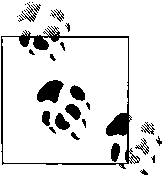
\includegraphics[width=2cm,clip]{paipai.png}
\end{wrapfigure}
\mbox{}过了相当长一段时间之后,ISO C99标准中增加了\_Exit()函数,它的功能和\_exit()是一样的:

\begin{lstlisting}
  #include <stdlib.h>
  void _Exit (int status);
\end{lstlisting}

\subsection{其他终止进程的方式}

终止进程的典型方式不是通过明确的使用一个系统调用,而是采用跳转到程序结尾处的方式。在C语言中,这发生在main()函数返回时。然而这种方式依然还是进行了系统调用:编译器会简单的在最后的代码中插入一个\_exit()。在main()函数返回时明确给出一个状态值,或者调用exit(),这是一个良好的编程习惯。shell会根据这个返回值来判断命令是否成功的执行了。注意,成功时的返回是exit(0),或者是从main()函数返回0。

如果进程收到一个信号,并且这个信号对应的处理函数是终止进程,进程也会终止。这样的信号包括SIGTERM 和 SIGKILL(参考第九章)。

最后一种是进程被内核惩罚性的终止。内核就会杀死执行非法指令,引起一个段错误,或者内存耗尽的进程。

\subsection{atexit()}

它是由POSIX 1003.1-2001所定义,并且Linux也实现了它。atexit()用来注册一些在进程结束时要调用的函数:

\begin{lstlisting}
  #include <stdlib.h>
  int atexit (void (*function)(void));
\end{lstlisting}

对atexit()的成功调用会把指定的函数注册到进程正常结束(例如一个进程以调用exit()或者从main()中返回的方式终止自己)时调用的函数中。如果进程调用了exec,所注册的函数列表会被清除(因为这些函数不存在于新进程的地址空间中)。如果进程是通过信号而结束的,这些注册的函数也不会被调用。

要注册的函数必须是无参数的,也没有返回值。它的原型应该像这样:

\begin{lstlisting}
  void my_function (void);
\end{lstlisting}

函数调用的顺序是和注册的顺序相反的。也就是这些函数存储在栈中,以后进先出的方式调用(LIFO)。注册的函数不能调用exit(),否则会引起无限的递归调用。如果需要提前结束进程,应该调用\_exit()。一般不推荐这样做,因为这样的会使得一些重要的函数不会被调用到。

POSIX标准要求atexit()至少支持注册ATEXIT\_MAX个函数,而这个值至少是32。具体的值可以通过sysconf( )得到,参数是\_SC\_ATEXIT\_MAX:

\begin{lstlisting}
  long atexit_max;
  atexit_max = sysconf (_SC_ATEXIT_MAX);
  printf ("atexit_max=%ld\n", atexit_max);
\end{lstlisting}

成功时,atexit()返回0。错误时返回-1。

这里是一个简单的例子:

\begin{lstlisting}
  #include <stdio.h>
  #include <stdlib.h>
  void out (void)
  {
    printf ("atexit( ) succeeded!\n");
  }
  int main (void)
  {
    if (atexit (out))
      fprintf(stderr, "atexit( ) failed!\n");
     return 0;
  }
\end{lstlisting}

\subsection{on\_exit( )}

SunOS 4定义自己的一个和atexit()等价的函数on\_exit(),Linux的glibc提供了对它的支持:

\begin{lstlisting}
  #include <stdlib.h>
  int on_exit (void (*function)(int , void *), void *arg);
\end{lstlisting}

这个函数的工作方式和atexit()一样,只是注册的函数原型不同:

\begin{lstlisting}
  void my_function (int status, void *arg);
\end{lstlisting}

参数status是传给exit()的值或者是main()函数返回的值。arg是传给on\_exit ()的第二个参数。必须小心的是当调用注册函数时,要保证arg所指的内存地址必须是有效的。

最新版本的Solaris不再支持这个函数了,应该使用标准的atexit()。

\subsection{SIGCHLD}

当一个进程子进程终止时,内核会向其父进程发送SIGCHILD信号。缺省情况下会忽略此信号量,父进程也不会有任何的动作。进程也可通过signal() 或 sigaction()系统调用来有选择的处理这个信号。这些系统调用和信号处理的部分会在第九章讲解。

SIGCHILD信号可能会在任何时候产生,也会在任何时候被传递给父进程。这是因为子进程的终止是和父进程异步的。通常情况下,父进程都希望能更多的了解到子进程的终止,或者显式的等待子进程的终止。与这些情况相关的系统调用会在下面讨论。

\section{等待终止的子进程}

用信号通知父进程是可以的,但是很多的父进程想知道关于子进程终止的更多信息——例如子进程的返回值。

如果在终止过程中,子进程完全消失了,就没有给父进程留下任何可以来了解子进程的东西。所以,Unix的设计者们做出了这样的决定:如果一个子进程在父进程之前结束,内核应该把子进程设置为一个特殊的状态。处于这种状态的进程叫做僵死(zombie)进程。进程只保留最小的概要信息——一些保存着有用信息的内核数据结构。僵死的进程等待这父进程来查询自己的信息(这叫做在僵死进程上等待)。只要父进程获取了子进程的信息,子进程就会消失,否则一直保持僵死状态。

Linux内核提供了一些接口来了解已经终止的子进程的信息。其中最简单的一个是wait(),它由POSIX所定义:

\begin{lstlisting}
  #include <sys/types.h>
  #include <sys/wait.h>
  pid_t wait (int *status);
\end{lstlisting}

wait()返回已终止子进程的pid,或者返回-1表示出错。如果没有子进程终止,调用者会被阻塞,直到一个子进程终止。如果子进程终止了,它就会立刻的返回。因此,响应子进程死亡的 wait () 调用(例如收到了 SIGCHILD 信号)不会被阻塞。

错误时,errno有两种可能的值:

\begin{eqlist*}
\item[\textbf{ECHILD}] 调用进程没有任何子进程。
\item[\textbf{EINTR}] 等待子进程结束时,收到了一个信号,wait()提前返回了。
\end{eqlist*}

如果status不是NULL,那么它包含了一些关于子进程的附加信息。因为POSIX允许实现时可以在status定义一些合适的bit位来表示附加信息。POSIX标准提供了一些宏来解释这些信息:

\begin{lstlisting}
  #include <sys/wait.h>
  int WIFEXITED (status);
  int WIFSIGNALED (status);
  int WIFSTOPPED (status);
  int WIFCONTINUED (status);
  int WEXITSTATUS (status);
  int WTERMSIG (status);
  int WSTOPSIG (status);
  int WCOREDUMP (status);
\end{lstlisting}

前两个宏会根据子进程的结束情况,可能会返回真(一个非零值)。如果进程正常结束了——也就是进程调用了\_exit( ),第一个宏WIFEXITED返回真。在这种情况下WEXITSTATUS返回传递给\_exit( )的低八位。

如果是信号(参看第九章对信号的讨论)引起进程的终止,WIFSIGNALED返回真。在这种情况下WTERMSIG返回引起进程终止的那个信号的编号。如果进程收到信号时发生了主存信息转储(dumped core),WCOREDUMP就返回true。尽管WCOREDUMP没有被POSIX定义,但是许多Unix系统,包括Linux都支持它。

如果子进程停止了或者继续执行,WIFSTOPPED和 WIFCONTINUED分别返回真。这些是通过ptrace()系统调用跟踪的。只有当实现一个调试器时,这些才有用。尽管有waitpid()(参看下面的讨论),但它们也是可以用来实现作业控制。wait()一般用来获取子进程的终止信息。如果WIFSTOPPED返回真,WSTOPSIG就返回使得进程停止的那个信号的编号。虽然POSIX没有定义WIFCONTINUED,但是新的标准把它定义为waitpid()。正如2.6.10内核中,Linux也为wait()提供了这个宏。

让我们来看看一个使用wait()来确定其子进程所发生的事:

\begin{lstlisting}
  #include <unistd.h>
  #include <stdio.h>
  #include <sys/types.h>
  #include <sys/wait.h>
  int main (void)
  {
    int status;
    pid_t pid;
    if (!fork ())
      return 1;
    pid = wait (&status);
    if (pid == -1)
      perror ("wait");
    printf ("pid=%d\n", pid);
    if (WIFEXITED (status))
      printf ("Normal termination with exit status=%d\n", WEXITSTATUS (status));
    if (WIFSIGNALED (status))
      printf ("Killed by signal=%d%s\n", WTERMSIG (status), WCOREDUMP (status) ? " (dumped core)" : "");
    if (WIFSTOPPED (status))
      printf ("Stopped by signal=%d\n", WSTOPSIG (status));
    if (WIFCONTINUED (status))
      printf ("Continued\n");
    return 0;
  }
\end{lstlisting}

在这个程序中,创建了一个子进程,它会立刻退出。父进程随后调用了wait()来获取子进程的状态。父进程会打印出子进程的pid以及结束信息。在这个例子中,子进程的结束是从main()返回,所以可以看到类似下面的输出:

\begin{verbatim}
  $ ./wait
  pid=8529
  Normal termination with exit status=1
\end{verbatim}

如果子进程的结束不是从main()返回,而是使它调用abort()(在<stdlib.h>中定义)——这会使子进程会向自己发送一个SIGABRT信号——那么我们看到的将是下面的输出:

\begin{verbatim}
  $ ./wait
  pid=8678
  Killed by signal=6
\end{verbatim}

\subsection{等待特定进程}

监视子进程的行为是很重要的。通常一个进程可能有很多子进程,但不需要等待所有子进程的结束,父进程只想等待其中一个特定的子进程。一种解决方式就是多次调用wait(),每次根据返回值来判断是不是那个特定的进程。这是十分笨拙的——假设这样一种情况,如果你要检测另一个子进程的状态呢?父进程必须保存所有wait()的返回值,以备将来会用到。

如果知道需要等待进程的pid,可以使用waitpid()系统调用:

\begin{lstlisting}
  #include <sys/types.h>
  #include <sys/wait.h>
  pid_t waitpid (pid_t pid, int *status, int options);
\end{lstlisting}

比起wait()来,waitpid()是一个更强大的系统调用。它额外的参数可以用来微调。

参数pid是需要等待的一个或多个进程的pid。它的值必须是下面四种情况之一:

\begin{eqlist*}
\item[\textbf{< -1}] 等待所有这样的子进程,它们的组ID是参数pid的绝对值。例如传递-500表示等待所有在进程组500中的所有子进程。
\item[\textbf{-1}] 等待任一子进程,这和wait()等效。
\item[\textbf{0}] 等待与调用进程处于同一进程组的任一进程。
\item[\textbf{>0}] 等待进程pid等于传入值的那个子进程。例如传递500表示等待pid为500的那个子进程。
\end{eqlist*}

参数status的作用和在wait()中的那个参数是一样的,并且前面的宏也是可以使用的。

参数options是零或多个下面选项按二进制“或”运算的结果:

\begin{eqlist*}
\item[\textbf{WNOHANG}]	如果要等待的子进程已经结束,或者停止,或者处于继续运行的状态,则waitpid()不会阻塞,它会立刻返回。
\item[\textbf{WUNTRACED}] 如果设置该位,即使是调用进程没有跟踪子进程,WIFSTOPPED也一样被设置。这个标志可以用来实现更通用的作业控制,例如shell。
\item[\textbf{WCONTINUED}] 如果设置该位,即使是调用进程没有跟踪子进程,WIFCONTINUED也一样被设置。 和 WUNTRACED一样,这个标志对于shell的实现很有帮助的。
\end{eqlist*}

调用成功时,waitpid()返回状态发生改变那个进程的pid。如果设置了WNOHANG参数,那么等待的那个(些)特定进程的状态没有改变就返回0。发生错误时,返回-1,并且errno的值会是下面三个中的一个:

\begin{eqlist*}
\item[\textbf{ECHILD}] 参数pid所指定的进程不存在,或者不是调用者的子进程。
\item[\textbf{EINTR}] 没有设置WNOHANG,而且在等待过程中收到了一个信号。
\item[\textbf{EINVAL}] 参数options不合法。
\end{eqlist*}

作为一个例子,假设你的程序想得到pid为1742的子进程的返回值,但是如果子进程没有结束,父进程就会立刻返回。也许你会写出和下面类似的代码:

\begin{lstlisting}
  int status;
  pid_t pid;
  pid = waitpid (1742, &status, WNOHANG);
  if (pid == -1)
    perror ("waitpid");
  else {
    printf ("pid=%d\n", pid);
    if (WIFEXITED (status))
      printf ("Normal termination with exit status=%d\n", WEXITSTATUS (status));
    if (WIFSIGNALED (status))
      printf ("Killed by signal=%d%s\n", WTERMSIG (status), WCOREDUMP (status) ? " (dumped core)" : "");
  }
\end{lstlisting}

作为最后一个例子,应该注意到下面wait()的用法:

\begin{lstlisting}
  wait (&status);
\end{lstlisting}

和这样使用waitpid()是一样的:

\begin{lstlisting}
  waitpid (-1, &status, 0);
\end{lstlisting}

\subsection{其他等待子进程的方法}

作为应用程序来说,它们希望有更多等待子进程的方式。XSI扩展了POSIX,而且Linux提供了waitid():

\begin{lstlisting}
  #include <sys/wait.h>
  int waitid (idtype_t idtype, id_t id, siginfo_t *infop, int options);
\end{lstlisting}

和wait()与waitpid()一样, waitid()作用是等待子进程的结束和了解子进程状态改变的信息(终止、停止或者继续运行)。它有更多的选项,但是这是以增加复杂性为代价的。

与waitpid()一样,waitid()允许程序员指定所要等待的子进程。但是为了完成这项工作,waitid()需要两个参数,而不是一个。参数idtype和id用来指定所要等待的子进程,这和waitpid()中的pid参数的作用一样。idtype的值是下面三个中的一个:

\begin{eqlist*}
\item[\textbf{P\_PID}] 等待pid值是id的子进程。
\item[\textbf{P\_GID}] 等待进程组ID是id那些子进程。
\item[\textbf{P\_ALL}] 等待所有子进程,参数id被忽略。
\end{eqlist*}

参数id是很少见的id\_t类型,这种类型代表着一种通用的ID号。因为将来可能会增加idtype的值,所以会引入这个类型。这样新加入的idtype值也可以被包容进去。id\_t类型是足够大的,保证了可以保存任何类型的pid\_t值。在Linux上,可以把它当做pid\_t来用——例如直接把类型为pid\_t的变量传递给它,或者数值性的常量。总之在编程上,不必担心类型的转化。

参数options是以下一个或者多个选项进行二进制''或''运算的结果:

\begin{eqlist*}
\item[\textbf{WEXITED}] 调用进程会等待结束的子进程(由id和idtyp指定)。
\item[\textbf{WSTOPPED}] 调用进程会等待收到了信号而停止了执行的子进程。
\item[\textbf{WCONTINUED}] 调用进程会等待收到了信号而继续执行的子进程。
\item[\textbf{WNOHANG}] 调用进程不会阻塞,如果没有子进程结束(停止或者继续执行),它就立刻返回。
\item[\textbf{WNOWAIT}] 调用进程不会移除满足条件的子进程的僵死状态。调用进程可能会在将来继续等待。
\end{eqlist*}

成功时,waitid()会填充参数infop,但是它必须指向一个有效的siginfo\_t类型。siginfo\_t结构体的具体成员是与实现相关的。\footnote[1]{实际上siginfo\_t结构体在Linux上是很复杂的。关于它的定义,参看/usr/include/bits/siginfo.h。我们会在第九章讨论关于它的更多细节。}但是还是有一些成员是在waitpid()调用之后还是有效的。也就是成功的调用会保证下面的成员会被填充:

\begin{eqlist*}
\item[\textbf{si\_pid}] 子进程的pid
\item[\textbf{si\_uid}] 子进程的uid
\item[\textbf{si\_code}] 根据子进程的状态是被信号所终止、杀死、停止或者继续执行而分别设置为CLD\_EXITED、CLD\_KILLED、 CLD\_STOPPED或者CLD\_CONTINUED中的一个。
\item[\textbf{si\_signo}] 设置为SIGCHLD。
\item[\textbf{si\_status}] 如果si\_code是CLD\_EXITED,它是子进程的退出值。否则,它引起状态改变的那个信号的编码。
\end{eqlist*}

当成功时,waitid()返回0。错误时,返回-1。errno会被设置成下列值之一:

\begin{eqlist*}
\item[\textbf{ECHLD}] 由id和idtype确定的进程不存在。
\item[\textbf{EINTR}] 一个信号打断了子进程的执行,但是在options里没有设置WNOHANG。
\item[\textbf{EINVAL}] options参数不合法,或者id和idtyp的组合不合法。
\end{eqlist*}

waitid()提供了比wait()和waitpid()更多有用的语义。尤其是可以从siginfo\_t结构体获取的信息是很有用的。如果不需要这些信息,那么就应该选择更简单的函数,这样可以被更多的系统所支持,并且可以更容易被移植到更多的非Linux的系统上。

\subsection{BSD中的wait3()和wait4()}
在waitpid()从AT\&T的System V Release 4诞生的同时,BSD采用自己的方法,提供了另外两个函数用于等待子进程的状态改变:

\begin{lstlisting}
  #include <sys/types.h>
  #include <sys/time.h>
  #include <sys/resource.h>
  #include <sys/wait.h>
  pid_t wait3 (int *status, int options, struct rusage *rusage);
  pid_t wait4 (pid_t pid, int *status, int options, struct rusage *rusage);
\end{lstlisting}

数字3和4实际上是指这两个函数分别有三个和四个参数。

除了rusage参数外,这两个函数的工作方式基本和waitpid()一致,下面对wait3()的调用:

\begin{lstlisting}
  pid = wait3 (status, options, NULL);
\end{lstlisting}

等价于下面的waitpid()调用:

\begin{lstlisting}
  pid = waitpid (-1, status, options);
\end{lstlisting}

并且下面对wait4()的调用:

\begin{lstlisting}
  pid = wait4 (pid, status, options, NULL);
\end{lstlisting}

等价于下面的waitpid()调用:

\begin{lstlisting}
  pid = waitpid (pid, status, options);
\end{lstlisting}

也就是wait3()等待着任何子进程改变状态,wait4()等待有pid所指定的子进程改变状态。参数options的作用和waitpid()中的一样。

前面就提到过,这些系统调用的最大不同就是rsuage参数。如果rsuage不是空,那么它所指的rsuage结构体会被填充上与子进程相关的信息。这个结构体提供了子进程资源的使用情况:

\begin{lstlisting}
  #include <sys/resource.h>
  struct rusage {
    struct timeval ru_utime; /* user time consumed */
    struct timeval ru_stime; /* system time consumed */
    long ru_maxrss;   /* maximum resident set size */
    long ru_ixrss;    /* shared memory size */
    long ru_idrss;    /* unshared data size */
    long ru_isrss;    /* unshared stack size */
    long ru_minflt;   /* page reclaims */
    long ru_majflt;   /* page faults */
    long ru_nswap;    /* swap operations */
    long ru_inblock;  /* block input operations */
    long ru_oublock;  /* block output operations */
    long ru_msgsnd;   /* messages sent */
    long ru_msgrcv;   /* messages received */
    long ru_nsignals; /* signals received */
    long ru_nvcsw;    /* voluntary context switches */
    long ru_nivcsw;   /* involuntary context switches */
  };
\end{lstlisting}

我们会在下一章讨论这些问题。

当成功调用时,返回0。错误时,返回-1。errno会被设置成和waitpid()一样的值。

因为wait3()和wait4()不是由POSIX所定义的,\footnote[1]{最初wait3()包含在Single UNIX Specification中,但后来被删除了}所以最好不要使用它们,除非真的需要了解子进程的资源使用情况。尽管它们不是有POSIX所定义的,但是几乎所有的UNIX系统都支持它们。

\subsection{创建并等待一个新进程}

ANSI和POSIX都定义了一个用于创建新进程并等待它结束的函数——可以把它想象成是同步的创建进程。如果一个进程创建了新进程然后就立刻开始等待它的结束,那么使用下面的函数就很合适:

\begin{lstlisting}
  #define _XOPEN_SOURCE    /* if we want WEXITSTATUS, etc. */
  #include <stdlib.h>
  int system (const char *command);
\end{lstlisting}

system()之所以这样命名是因为进程同步创建一般被称为''交付给系统运行''。使用system()来运行一个简单的工具程序或者shell脚本是很常见的,大多数都是希望得到工具程序或者脚本的返回值。

对system()的调用会使得由参数command指定的程序的得到执行,而且程序可以得到相应的参数。''/bin/sh –c''会作为前缀加到command参数前面。这样才会将整个参数传递给shell。

成功时,返回值是执行命令得到的返回状态,该状态与wait提供的一致。接下来执行命令的返回值会通过WEXITSTATUS得到。如果对/bin/sh自己的调用失败了,那么从WEXITSTATUS得到的值和调用exit(127)的返回值是一样的。也可能调用的命令返回了127,但是没有办法来检测是不是shell自己发生了错误而返回的127。system()调用失败时返回-1。

如果参数command是NULL且/bin/sh是可用的,system()返回一个非零的值,其他情况返回0。

在命令执行的过程中,SIGCHILD信号是被阻塞的,而且SIGINT和SIGQUIT信号会被忽略。实现对SIGINT和SIGQUIT信号的忽略有好几种实现方式,特别是当system()在循环中被调用的时候。如果在一个循环中调用system(),那么你需要保证子进程的退出状态要被正确检测。例如:

\begin{lstlisting}
  do {
    int ret;
    ret = system ("pidof rudderd");
    if (WIFSIGNALED (ret) && (WTERMSIG (ret) == SIGINT || WTERMSIG (ret) == SIGQUIT))
      break; /* or otherwise handle */
  } while (1);
\end{lstlisting}

利用fork()、exec系统调用和waitpid()实现一个system()是非常有用的练习。你应该自己尝试一下,因为它融合了本章中的许多概念。为了完整性,这里有一个简单的实现:

\begin{lstlisting}
 /*
  * my_system - synchronously spawns and waits for the command
  * "/bin/sh -c <cmd>".
  *
  * Returns -1 on error of any sort, or the exit code from the
  * launched process. Does not block or ignore any signals.
  */
  int my_system (const char *cmd)
  {
    int status;
    pid_t pid;
    pid = fork ( );
    if (pid == -1)
      return -1;
    else if (pid == 0) {
      const char *argv[4];
      argv[0] = "sh";
      argv[1] = "-c";
      argv[2] = cmd;
      argv[3] = NULL;
      execv ("/bin/sh", argv);
      exit (-1);
    }
    if (waitpid (pid, &status, 0) == -1)
      return -1;
    else if (WIFEXITED (status))
      return WEXITSTATUS (status);
    return -1;
  }
\end{lstlisting}

注意这个例子不像正式的system(),它没有阻塞或者禁止任何信号。根据你程序的情况,这可能是好事也可能是坏事。但是至少要保证SIGINT信号不被阻塞,这是很明智的,因为这样可以按照用户的意愿随时终止命令的执行。一个较好的实现可以将额外的指针做为参数,当参数为非空时,代表不同的错误。例如可能会加入fork\_failed 和shell\_failed。

\subsection{僵死进程}

正如前面提到到的那样,一个进程已经终止了,但是它的父进程还在等待获得它状态,那么这个进程就叫做僵死进程。僵死进程还会消耗一些系统资源,尽管这些资源很少——仅仅够描述进程曾经的状态。这些保留的资源主要是为了在父进程查询子进程的状态时提供相应的信息。一旦父进程得到了想要的信息,内核就会清除这些信息,僵死的进程就不存在了。

然而任何用过Unix系统的人都会或多或少的看到过僵死进程。通常这些进程叫做鬼魂进程(ghosts),这些进程没有相应的父进程。如果你的进程创建了一个子进程,那么它就有责任去等待子进程(除非它的生命周期很短,这种情况你很快就会看到),即使它会丢弃得到的子进程的信息。否则你的这些子进程会称为鬼魂进程,并一直存在。它们充斥在系统的进程列表中,使你的应用程序看起来非常讨厌.

然而如果父进程在子进程结束之前就结束了呢?或者父进程还没有机会等待僵死的子进程,它就先结束了呢?无论何时,只要有进程结束了,内核就会遍历它的所有子进程,并且把它们的父进程重新设为init进程(pid为1的那个进程)。这保证了系统中不存在没有父进程的进程。init进程会周期性的等待所有子进程,确保不会有长时间存在的僵死进程——没有鬼魂进程。因而当父进程在子进程之前结束了,或者在退出前没有等待子进程,那么init进程会被指定为这些子进程的父进程,从而确保了它们会完全的退出。这是一种非常好的处理方式,这种安全措施也意味着生命周期短的进程没有必要等待它所有的子进程结束。

\section{用户和组}

正如本章前面和第一章中所讨论过的,进程是与用户和组相关联的。用户ID和组ID分别用C语言的uid\_t和gid\_t这两个类型表示。数字表示和可读字符串之间的映射关系(例如root用户的uid是0)是通过用户空间的/etc/passwd 和/etc/group两个文件完成的。内核只处理数字表示的形式。

在Linux系统中,一个进程的用户ID和组ID代表这个进程可以执行哪些操作。进程必须以合适的用户和组运行。许多的进程是以root用户运行着的。然而,最好的方式就是采取“最小权限”的原则,它意味着进程要尽可的以最小的权限来运行。这个要求是动态变化的:如果进程在前期需要以root用户的权限运行,而在后面不需要root权限了,那么它就应该在后期尽可能的放弃root权限。总之,许多进程——特别是那些不需要root权限来执行一些操作时——经常需要操作自己的用户ID或者组ID。

但是在我们具体了解如何实现之前,我们需要了解一些用户ID和组ID的复杂性。

\subsection{实际用户(组)ID、有效用户(组)ID和保存设置的用户(组)ID}

\begin{wrapfigure}{l}{2.5cm}
  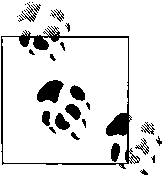
\includegraphics[width=2cm,clip]{paipai.png}
\end{wrapfigure}
\mbox{}下面的讨论会集中在用户ID上,但组ID的情况是一样的。

实际上,与进程相关的用户ID有四个而不是一个,它们是:实际用户ID、有效用户ID、保存设置的用户ID和文件系统用户ID。实际用户ID是运行这个进程的那个用户的uid。这个用户的uid会被设置为父进程的实际用户ID,并且在exec系统调用中不会发生改变。一般情况下,登陆进程会将用户登陆的那个shell的实际用户ID设置为用户的ID,并且这个用户所有进程的实际用户ID都会继承这个值。超级用户(root)可能会把实际用户ID该为任意的值,但是其他用户是不能改变这个值的。

有效用户ID是当前进程所使用的用户ID。权限验证一般是使用这个值。初始时,这个ID等于实际用户ID。因为创建进程时,子进程会继承父进程的有效用户ID。更进一步的讲,exec系统调用不会改变有效用户ID。但是在exec调用过程中,实际用户ID和有效用户ID的主要区别出现了:通过setuid (suid)程序,进程可以改变自己的有效用户ID。准确的说,有效用户ID被设置为拥有此程序文件拥有者的用户ID。比如,/usr/bin/passwd是一个setuid文件,它的所有者是root用户。当一个普通用户创建一个进程来运行它,不论谁运行了它,这个进程的有效用户ID就是root用户的ID。

你立刻会看到,非特权用户只能把有效用户ID设置成实际用户ID或保存设置的用户ID。超级用户可以把有效用户ID设置成任何值。

保存设置的用户ID是进程原先的有效用户ID。当创建进程时,子进程会从父进程继承保存设置的用户ID。对于exec系统调用来说,内核会把保存设置的用户ID设置为有效用户ID,从而在exex系统调用过程中保存了一份有效用户ID的记录。非特权用户不能改变保存设置的用户ID的值,超级用户可以把它设置为实际用户ID的值。

为什么会有这么多的ID呢?有效用户ID的作用是:它是在检查进程权限过程中使用的用户ID。实际用户ID和保存设置的用户ID像是代理或者一个潜在的用户ID值,它的作用是允许非root进程在这些用户ID之间相互切换。实际用户ID是真正运行程序的有效用户id。保存设置的用户ID是在执行suid程序前的有效用户id。

\subsection{改变实际用户(组)ID和保存设置的用户(组)ID}

用户ID和组ID是通过下面两个系统调用设定的:

\begin{lstlisting}
  #include <sys/types.h>
  #include <unistd.h>
  int setuid (uid_t uid);
  int setgid (gid_t gid);
\end{lstlisting}

seteuid()用来设定当前进程的有效用户ID。如果进程当前的有效用户ID是0(root),那么实际用户ID和保存设置的用户ID的值也会被同时设置。root用户可以为uid提供任何值,从而将所有三种用户ID的值设置为了uid。非root用户只允许将实际用户ID和保存设置的用户ID设置为uid。也就是,非root用户只能将有效用户ID设置为上述中的一个值。

调用成功时,setuid()返回0。错误时,返回-1,并把errno设置为下面的值之一:

\begin{eqlist*}
\item[\textbf{EAGAIN}] uid的值和实际用户ID的值不同,把实际用户ID的值的改变为uid会导致此用户超过NPROC的限制(它定义了一个用户可以拥有的进程数)。
\item[\textbf{EPERM}] 不是root用户,uid既不是有效用户ID也不是保存设置的用户ID。
\end{eqlist*}

前面的讨论对组依然是适用的,只需要将setuid()替换为setgid(),把uid替换为gid。

\subsection{改变有效用户和组ID}

Linux提供了两个POSIX所定义的函数来改变当前进程的有效用户id和组ID的值:

\begin{lstlisting}
  #include <sys/types.h>
  #include <unistd.h>
  int seteuid (uid_t euid);
  int setegid (gid_t egid);
\end{lstlisting}

setuid()的调用将有效用户ID的值设置为euid。root用户可以为euid提供任何值。而非root用户只能将有效用户ID设置为有效用户ID或者是保存设置的用户ID。成功时,setuid()返回0,失败时返回-1,并把errno设置为EPERM。它表示当前进程的所有者不是root用户,并且euid的值既不等于实际用户ID也不等于保存设置的用户ID。

注意,对于非root用户来说,seteuid() 和setuid()是一样的。所以总是使用seteuid()是不错的选择。如果你的进程要以root权限来运行,那么使用setuid()就更合适一些。

前面的讨论对组依然是适用的,只需要将seteuid()替换为setegid(),把euid替换为egid。

\subsection{BSD改变用户ID和组ID的方式}

BSD在改变用户ID和组ID上有自己的接口。出于兼容性考虑,Linux也提供了这些接口:

\begin{lstlisting}
  #include <sys/types.h>
  #include <unistd.h>
  int setreuid (uid_t ruid, uid_t euid);
  int setregid (gid_t rgid, gid_t egid);
\end{lstlisting}

调用setreuid()会分别将实际用户ID和有效用户ID分别设置为ruid和euid。将这两个参数中的任何一个设置为-1表示着不会改变相应的用户ID。非root用户只允许将有效用户ID设置为实际用户ID或者是保存设置的用户ID,和把实际用户ID设置为有效用户ID。如果实际用户ID改变了,或者要把有效用户ID设置为不是先前的实际用户ID的值,再或者要把保存设置的用户ID设置为新的有效用户ID,那么这些行为是由Linux或者其他Unix系统自己所决定的。在POSIX中,这些都是未定义的行为。

成功时,setreuid()返回0,错误时返回-1,并把errno设置为EPERM。它表示当前进程的所有者不是root用户,并且euid的值即不等于实际用户ID也不等于保存设置的用户ID,或者ruid不等于有效用户ID。

前面的讨论对组依然是适用的,只需要将setreuid()替换为setregid(),把ruid替换为rgid,把euid替换为egid。

\subsection{HP-UX中改变用户ID和组ID的方式}

你可能已经感到形式已经有些混乱了,但是HP-UX(Hewlett-Packard’s Unix系统)也有自己设定用户ID和组ID的方式。Linux同样提供了这些接口:

\begin{lstlisting}
  #define _GNU_SOURCE
  #include <unistd.h>
  int setresuid (uid_t ruid, uid_t euid, uid_t suid);
  int setresgid (gid_t rgid, gid_t egid, gid_t sgid);
\end{lstlisting}

调用setresuid()会分别将实际用户ID、有效用户ID和保存设置的用户ID分别设置为ruid、euid和suid。将这几个参数中的任何一个设置为-1表示着不会改变相应的用户ID。

root用户可以把任何用户ID设置为任何值。非root用户只可以把用户ID设为当前的实际用户ID、有效用户ID和保存设置的用户ID。成功时,setresuid()(原文有误)返回0,错误时返回0,并把errno设置为下列值之一:

\begin{eqlist*}
\item[\textbf{EAGAIN}] uid的值和实际用户ID的值不同,把实际用户ID的值改变为uid会导致此用户超过NPROC的限制(它定义了一个用户可以拥有的进程数)。
\item[\textbf{EPERM}] 不是root用户,并且设置的新的实际用户 ID、有效用户ID或保存设置的用户 ID,不匹配当前的实际用户 ID、有效用户ID或保存设置的用户ID。
\end{eqlist*}

前面的讨论对组依然是适用的,只需要将setresuid()替换为setresgid (),把ruid替换为rgid,把euid替换为egid,把suid替换为sgid。

\subsection{操作用户ID组ID的首选方法}

非root用户应该使用seteuid()来设置有效用户ID。如果有root权限的进程希望改变三种用户ID,那么应该使用setuid();而只是想临时改变有效用户ID,那么最好使用seteuid()。这些函数是很简单的,它们的行为遵从POSIX中的定义,并且在适当的时候考虑用一下保存设置的用户ID。

除了提供额外的功能,BSD和HP-UX并没有允许作出setuid()和seteuid()所没有的改变。

\subsection{对保存设置的用户ID的支持}

保存设置的用户ID是IEEE Std 1003.1-2001(POSIX 2001)中出现的,Linux早在1.1.38内核时就提供了相应的支持。仅为Linux编写的程序可以放心使用保存设置的用户id。为较较老版本的Unix编写的程序在引用保存用户设置的用户id或组id之前需要检查一下\_POSIX\_SAVED\_IDS宏。

对于不支持保持设置的用户ID和组ID的系统,上面的讨论依然是成立的。只需要忽略前面与保持设置的用户ID和组ID的相关讨论即可。

\subsection{获取用户ID和组ID}

下面的两个系统调用分别返回实际用户ID和组ID:

\begin{lstlisting}
  #include <unistd.h>
  #include <sys/types.h>
  uid_t getuid (void);
  gid_t getgid (void);
\end{lstlisting}

它们不能失败。相应的下面两个系统调用分别返回有效用户ID和组ID:

\begin{lstlisting}
  #include <unistd.h>
  #include <sys/types.h>
  uid_t geteuid (void);
  gid_t getegid (void);
\end{lstlisting}

这两个系统调用同样不能失败。

\section{会话和进程组}

每个进程都属于某个进程组。进程组是由一个或多个相互间有关联的进程组成的,它的目的是为了进行作业控制。进程组的主要特征就是信号可以发送给进程组中的所有进程:这个信号可以使同一个进程组中的所有进程终止、停止或者继续运行。

每个进程组都由进程组ID(pgid)唯一的标识,并且有一个组长进程。进程组ID就是组长进程的pid。只要在某个进程组中还有一个进程存在,则该进程组就存在。即使组长进程终止了,该进程组依然存在。

当有新的用户登陆计算机,登陆进程就会为这个用户创建一个新的会话。这个会话中只有用户的登陆shell一个进程。登陆shell做为会话首进程(session leader)。会话首进程的pid就被作为会话的ID。一个会话就是一个或多个进程组的集合。会话囊括了登陆用户的所有活动,并且分配给用户一个控制终端(controling terminal)。控制终端是一个用于处理用户I/O的tty设备。因此,会话的功能和shell差不多。没有谁刻意去区分它们。

进程组提供了向其中所有进程发送信号的机制,这使得作业控制和其他的shell功能变得很容易。同时会话则将登录与控制终端联系起来。会话中的进程组分为一个前台进程组和零个或多个后台进程组。当用户退出终端时,向前台进程组中的所有进程发送SIGQUIT信号。当出现网络中断的情况时,向前台进程组中的所有进程发送SIGHUP信号。当用户敲入了终止键(一般是Ctrl+C),向前台进程组中的所有进程发送SIGINT信号。因此,会话可以更容易的管理终端以及在shell上的登录行为。

让我们回顾一下以上的知识,假设某个用户登陆系统,他的登陆的shell是bash ,并且pid是1700。那么登陆的shell现在就是新进程组中唯一的进程,也是组长进程。这个进程组所在会话的会话ID是1700,并且shell是这个会话中的唯一成员,也是会话首进程。进程组中直接与用户打交道并且控制终端为前台进程组,其他的都是后台进程组。

在一个指定的系统中,存在着多个会话:每个用户的登陆都是一个会话,还有一些与用户登陆会话无关的进程也是会话(例如守护进程)。守护进程会创建自己的会话,从而避免与其他存在的会话产生关系。

这些会话都包含着一个或多个进程组,并且每个进程组至少有一个进程。而有多个进程的进程组通常是用来完成作业控制的。

\begin{verbatim}
  $ cat ship-inventory.txt | grep booty | sort
\end{verbatim}

以上这样一条shell命令会产生由三个进程构成的一个进程组。以这种方式,shell可以向三个进程同时发送信号。因为用户直接敲入了这条命令,结尾没有使用''\&'',所以它是一个前台进程组。图5-1显示了会话、进程组、进程和控制终端之间的关系。

\begin{figure}[htp]
  \centering
  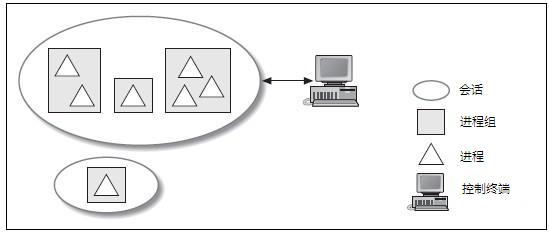
\includegraphics[width=\textwidth]{ch5.jpg}
  \caption{会话、进程组、进程及控制终端之间的关系}
\end{figure}
 
Linux提供了几个用来获取和设置与一个进程相关的会话进程组的接口。它们主要是为shell服务的,但是也可用于像守护进程之类的进程,因为守护进程不希望与与会话和进程组扯上关系。

\subsection{与会话相关的系统调用}

在登陆时,shell会创建新的会话。这是通过一个特殊的系统调用完成的,用它可以很容易的创建一个会话:

\begin{lstlisting}
  #include <unistd.h>
  pid_t setsid (void);
\end{lstlisting}

假如调用进程不是某个进程组组长进程,调用setsid()会创建新的会话。调用进程就是这个会话的唯一进程,也是新会话的首进程,但是它没有控制终端。调用也同时在这个会话中创建一个进程组,调用进程成为了组长进程,也是进程组中的唯一进程。新会话ID和进程组ID被设置为调用进程的pid。

也就是说,setsid()创建的新会话,并在其中创建一个新的进程组,而且使得调用进程成为新会话的首进程和新进程组的组长进程。对于守护进程来说,这十分有用,因为它不想是任何已存在会话的成员,也不想拥有控制终端。对于shell来说,它也很有用,因为shell希望为每一个登陆的用户创建新的会话。

成功调用,setsid()返回新会话的会话ID。错误时,返回-1,并把errno设置为EPERM,表示调用进程是是当前进程组的组长进程。有一个简单的方法可以使得任何进程不成为组长进程。这就是创建一个新进程,终止父进程,让子进程来调用setsid()。例如:

\begin{lstlisting}
  pid_t pid;
  pid = fork ();
  if (pid == -1) {
    perror ("fork");
    return -1;
  } else if (pid != 0)
    exit (EXIT_SUCCESS);
  if (setsid ( ) == -1) {
    perror ("setsid");
    return -1;
  }
\end{lstlisting}

虽然获得当前进程的会话ID不是很常用,但是也是可以做到的:

\begin{lstlisting}
  #define _XOPEN_SOURCE 500
  #include <unistd.h>
  pid_t getsid (pid_t pid);
\end{lstlisting}

对getsid()的调用会返回pid进程的会话ID。如果参数pid是0,就返回调用进程的会话ID。错误时,返回-1。而errno的唯一可能值就是ESRCH,表示pid不代表任何进程。注意,其他UNIX系统会把errno设置为EPREM,它表示pid指示的进程和调用进程不属于同一个会话。Linux不会这么处理,它倾向于返回任何进程的会话ID。

getsid()是很少使用的,且主要用于诊断问题:

\begin{lstlisting}
  pid_t sid;
  sid = getsid (0);
  if (sid == -1)
    perror ("getsid"); /* should not be possible */
  else
    printf ("My session id=%d\n", sid);
\end{lstlisting}

\subsection{与进程组相关的系统调用}

setpgid()将pid进程的进程组ID设置为pgid:

\begin{lstlisting}
  #define _XOPEN_SOURCE 500
  #include <unistd.h>
  int setpgid (pid_t pid, pid_t pgid);
\end{lstlisting}

如果pid是0,则使用调用者的进程ID。如果pgid是0,则将pid的进程ID设置为进程组ID。

成功时,返回0。它必须依赖几个条件:

\begin{itemize}
\item pid代表的进程必须是调用者或者是其子进程,而且子进程没有调用过exec函数,并且pid进程和调用者在同一个会话中。
\item pid进程不能是会话首进程。
\item 如果pgid已经存在,那么必须与调用者在同一个会话中。
\item pgid非负。
\end{itemize}

错误时,返回-1,并把errno设置为下列值之一:

\begin{eqlist*}
\item[\textbf{EACCESS}] pid进程是调用进程的子进程,且调用进程调用了exec函数。
\item[\textbf{EINVAL}] pgid小于0。
\item[\textbf{EPERM}] pid进程是会话首进程,或者是与调用者不在同一个会话中的另一个进程。也可能是试图将进程放置到一个不在同一个会话的进程组中。
\item[\textbf{ESRCH}] pid不是当前进程或0或当前进程的子进程。
\end{eqlist*}

尽管不是很常用,还是可以通过会话获得进程的进程组ID:

\begin{lstlisting}
  #define _XOPEN_SOURCE 500
  #include <unistd.h>
  pid_t getpgid (pid_t pid);
\end{lstlisting}

getpgid()返回pid进程的进程组ID。如果pid是0,返回当前进程的进程组ID。出错则返回-1,而errno的唯一值是ERSCH,表示pid是一个非法的进程标识符。

与getsid()类似,getpgid也主要用于诊断错误:

\begin{lstlisting}
  pid_t pgid;
  pgid = getpgid (0);
  if (pgid == -1)
    perror ("getpgid"); /* should not be possible */
  else
    printf ("My process group id=%d\n", pgid);
\end{lstlisting}

\subsection{废弃的进程组函数}

Linux支持BSD中两个较早的用于操作和获取进程组ID的接口。因为它们不如前面讨论的系统调用常用了,除非对可移植性有要求,新的程序应该不使用它们。setpgrp()用来设置进程组ID:

\begin{lstlisting}
  #include <unistd.h>
  int setpgrp (void);
\end{lstlisting}

这样的调用:

\begin{lstlisting}
  if (setpgrp ( ) == -1)
    perror ("setpgrp");
\end{lstlisting}

和下面的调用是一样的:

\begin{lstlisting}
  if (setpgid (0,0) == -1)
    perror ("setpgid");
\end{lstlisting}

两个都试图把进程组ID设置为当前进程的进程ID。成功时返回0,失败时返回-1。除了ERSCH,setpgid()的所有errno可能值都适用于setpgrp()。

同样的,getpgrp()用来获取进程组ID:

\begin{lstlisting}
  #include <unistd.h>
  pid_t getpgrp (void);
\end{lstlisting}

这样的调用:

\begin{lstlisting}
  pid_t pgid = getpgrp ( );
\end{lstlisting}

和下面的是一样的:
\begin{lstlisting}
  pid_t pgid = getpgid (0);
\end{lstlisting}

两者都返回调用进程的进程组ID。getpgid()不能失败。

\section{守护进程}

守护进程运行在后台,不与任何控制终端相关联。守护进程通常在系统启动时就运行,它们以root用户运行或者其他特殊的用户(例如apache和postfix),并处理一些系统级的任务。习惯上守护进程的名字通常以d结尾(就像crond和sshd),但这不是必须的,甚至不是通用的。

这个名字来源于麦克斯韦妖(Maxwell’s demon),它是物理学家James Maxwell在1867年进行的一个思想实验。Daemon这个词也是希腊神话中的鬼怪,它存在与人类和神之间,拥有占卜的能力。与Judeo-Christian神话中的daemon不同,希腊神话中的daemon不是邪恶的。实际上,神话中的daemon是神的助手,做一些奥林匹斯山的居民自己不愿做的事——很像Unix中的守护进程,完成前台用户不愿做的事。

对于守护进程有两个基本要求:它必须是init进程的子进程,并且不与任何控制终端相关联。

一般来讲,进程可以通过以下步骤成为守护进程:

\begin{enumerate}
\item 调用fork(),创建新的进程,它会是将来的守护进程。
\item 在守护进程的父进程中调用exit()。这保证了祖父进程(守护进程的祖父进程)确认父进程已经结束。还保证了父进程不再继续运行,守护进程不是组长进程。最后一点是顺利完成以下步骤的前提。
\item 调用setsid(),使得守护进程有一个新的进程组和新的会话,两者都把它作为首进程。这也保证它不会与控制终端相关联(因为进程刚刚创建了新的会话,同时也就不会为其关联一个控制终端)。
\item 用chdir( )将当前工作目录改为根目录。因为前面调用fork()创建了新进程,它所继承来的当前工作目录可能在文件系统中任何地方。而守护进程通常在系统启动时运行,同时不希望一些随机目录保持打开状态,也就阻止了管理员卸载守护进程工作目录所在的那个文件系统。
\item 关闭所有的文件描述符。不需要继承任何打开的文件描述符,对于无法确认的文件描述符,让它们继续处于打开状态。
\item 打开0、1和2号文件描述符(标准输入、标准输出和标准错误),把它们重定向到/dev/null。
\end{enumerate}

根据这些规则,下面的程序可以成为守护进程:

\begin{lstlisting}
  #include <sys/types.h>
  #include <sys/stat.h>
  #include <stdlib.h>
  #include <stdio.h>
  #include <fcntl.h>
  #include <unistd.h>
  #include <linux/fs.h>
  int main (void)
  {
    pid_t pid;
    int i;
    /* create new process */
    pid = fork ( );
    if (pid == -1)
      return -1;
    else if (pid != 0)
      exit (EXIT_SUCCESS);
    /* create new session and process group */
    if (setsid ( ) == -1)
      return -1;
    /* set the working directory to the root directory */
    if (chdir ("/") == -1)
      return -1;
    /* close all open files--NR_OPEN is overkill, but works */
    for (i = 0; i < NR_OPEN; i++)
      close (i);
    /* redirect fd's 0,1,2 to /dev/null */
    open ("/dev/null", O_RDWR);     /* stdin */
    dup (0);                        /* stdout */
    dup (0);                        /* stderror */
    /* do its daemon thing... */
    return 0;
  }
\end{lstlisting}

许多Unix系统在它们的C函数库中提供了daemon()函数来完成这些工作,将繁琐的工作简化了很多:

\begin{lstlisting}
  #include <unistd.h>
  int daemon (int nochdir, int noclose);
\end{lstlisting}

如果nochdir非零,就不会将工作目录改为根目录。如果noclose非零,就不关闭所有打开的文件描述符。如果父进程设置了守护进程的这些属性,那么这些参数是很有用的。通常都会把这些参数设为0。

成功时,返回0。失败时返回-1。errno设置为fork()或者setsid()的错误代码之一。

\section{总结}

在本章中,我们讲解了Unix系统中进程管理的基本知识,包括了从进程的创建到进程的终止。下一章,我们会讲解一些高级进程管理的API,例如改变进程调度方式的的API。

\ifx\atempxetex\usewhat
\XeTeXinputencoding "utf-8"
\fi
\defaultfont

\chapter{高级进程管理}

在第五章,我们介绍了进程的基本概念,讨论了创建、控制和销毁进程的内核接口。基于这些知识,本章将首先讨论Linux进程调度器及其调度算法,然后描述高级进程管理接口。这些系统调用控制进程的调度语义和行为,从而影响调度器为实现应用或者用户特定需求所作出的决策。

\section{进程调度}

进程调度器是内核中决定哪个进程可以运行的组件,换句话说,进程调度器简称------调度器------是把有限的处理器资源分配给进程的内核子系统。在作出决策的过程中,调度器既要最大化处理器效率,又要让多个进程同时运行、互不影响。

本章,我们会着重讨论“就绪进程”\footnote[1]{译者注:原文 runnable process}。它最重要的特征是该进程是非阻塞的。进行用户交互、大量读写文件、响应I/O和网络事件的进程会花费大量时间来等待资源可用,在相当长的时间内无法转为就绪状态(长是相对于指令运行时间而言),因此就绪进程首先应该是非阻塞的。一个就绪进程还必须至少有部分“时间片”(调度器分配给进程的运行时间)。内核用一个就绪队列维护所有的就绪进程,一旦某进程耗光它的时间片,内核就将其移出队列,直到所有就绪进程都耗光时间片才考虑将其放回队列。

如果只有一个就绪进程(甚至一个也没有),调度器就没有什么意义。只有在进程数多于处理器时,调度器才能体现它的价值。在这种情况下,显然有一些进程会等待其他进程运行;决定哪个进程运行,何时运行,运行多长时间也就成了调度器的基本责任。

一个操作系统能在单处理机上交错地运行多个进程,让人感到似乎同时运行多个进程,就称该操作系统是“多任务”的。在多处理机上,多任务操作系统允许进程在不同处理器上并行执行。非多任务操作系统,比如DOS,一次只能运行一个任务。

多任务操作系统分为两大类:协同式和抢占式。Linux实现了后一种形式的多任务,调度器可以要求一个进程停止运行,处理器转而运行另一个进程。这种中止正在运行的进程的行为称做抢占,类似的,进程在被抢占前所运行的时间称之为进程时间片(得名于调度器分配给每个就绪进程的一小片时间)。

在协同多任务系统中,一个进程持续运行直到它自发停止。我们称进程自发停止的行为为让出。理想情况下,会经常发生进程让出,但操作系统绝不可强制要求其让出。因此,一个拙劣或损坏的程序可能运行很长时间,甚至导致整个系统死掉。由于这个原因,现代操作系统几乎都采用抢占多任务机制,Linux也不例外。

2.5内核引入的O(1)进程调度器,是Linux调度\footnote[1]{对于好奇的读者,可以查看内核代码树中的 kernel/sched.c 文件了解细节}的核心。Linux调度算法采用抢占多任务机制,支持多处理器,处理器亲和度,非一致内存访问(NUMA),实时进程和用户自定义优先级等特性。

\subsection{大O记法}
O(1)是大O记法的一个例子,常用来表示算法的复杂性和可扩展性。形式地定义:
\begin{center}
  if f(x) is O(g(x)),

  then

  $\exists c,x'$ such that $f(x) \le c * g(x), \forall x > x'$
\end{center}

也就是说,一些算法的代价,以f表示,只要x大于某个初始值$x'$,f就一定小于等于g乘上一个常数,即g大于等于f,g是f的上界。

O(1)也就表明解决问题的代价小于常数c,这就带来极好的保证:无论系统中有多少进程,Linux进程调度器表现如一。对于调度器来说,选择一个新进程来运行至少需要迭代一次进程队列,因而O(1)算法对性能非常重要。在稍简单些的调度器中(包括以前版本的Linux调度器),随着进程数量的增长,进程队列的迭代会成为潜在的瓶颈。在最好情况下,也会给进程调度带来不确定性。

Linux调度器,在常数时间内运行,不会受到其他因素影响,就没有这样的瓶颈。

\subsection{时间片}

Linux分配给进程的时间片长短对于系统行为和性能非常重要。如果时间片太长,进程必须等待很长时间才能运行,这减小了运行的并行性,用户会察觉到明显的延迟;相反的,时间片太短,大量时间会花费在进程调度上,程序的时间局部性等也不能得到保证。

因而,确定合适的时间片绝非易事。一些系统给予进程长时间片,希望最大化系统吞吐率和整体表现。另一些系统给予较短的时间片,希望获得优秀的交互性能。我们将看到,Linux通过动态分配进程时间片,期望在两方面都做到最好。

注意:进程不一定要在一次运行中耗光所有时间片。一个被分配100ms时间片的进程,可能运行20ms就因为等待键盘输入等资源而阻塞。此时,调度器就会临时地把该进程移出就绪队列;当资源可用后,这个例子中是键盘缓冲区不为空,调度器会唤醒进程。进程会继续运行,耗光剩下的80ms或者又一次阻塞。

\subsection{I/O约束进程 Vs. 处理器约束进程}

持续地消耗所有可用时间片的进程称为“处理器约束进程”\footnote[1]{process-bound}。这类进程渴望CPU时间,消耗掉调度器分配的全部时间。最简单的例子就是无限循环,其他的例子包括科学计算,数学演算和图像处理。

另一方面,多数时间处于等待资源的阻塞状态的进程称为“I/O约束进程”\footnote[2]{I/O-bound}。I/O约束进程经常发起和等待文件I/O,阻塞在键盘输入,或者用户移动鼠标。I/O阻塞程序的例子包括文件实用程序,比如 cp 或者 mv,它们除了请求内核执行I/O操作外,几乎什么也不做;还包括GUI应用程序,大多数时候都在等待用户输入。

处理器约束程序和I/O约束程序得益于调度器对于不同程序类型所采用的不同行为。处理器约束程序得到尽可能长的时间片,从而最大化缓存命中率(时间局部性所致),尽快完成任务。相反地,I/O约束程序不需要长时间片,因为它们一般在发出I/O请求和阻塞在内核资源前只会运行很短的一段时间。然而,I/O约束程序也能从调度器的持久关注中获益。被唤醒地越快,可调度的I/O请求越多,程序越能够充分地利用系统硬件。更进一步,如果一个在等待用户输入的程序被调度的速度越快,给用户无缝运行的感觉越明显。

平衡处理器约束程序和I/O约束程序的不同需要绝非易事。Linux调度器试图识别和优先对待I/O约束程序:频繁I/O程序增加优先级,处理器约束程序减少优先级。

实际上,很多应用程序是处理器约束和I/O约束的混合体。音频视频解码编码就是一个好例子,许多游戏也是如此。因此对于一个给定程序,不总是能够判定它的倾向,在任意时间,进程都可能有不同的表现。

\subsection{抢占调度}

当一个进程耗光时间片的时候,调度器会中止其运行,开始运行一个新的进程。如果没有其他的就绪进程,内核会给予所有耗光时间片的进程新的时间片,继续运行。这样,即使系统中有高优先级进程---低优先级进程必须等待高优先级进程耗光时间片或者阻塞,所有的进程最终都会运行。这就明确描述了Unix调度中一条不起眼但是非常重要的原则: 所有的进程都必须运行。

如果没有就绪进程,内核会“运行”空闲进程(idle process)。实际上,空闲进程既不是一个进程,也不能实际运行(减少电池消耗)。空闲进程是为了简化调度算法和统计方便而生的特殊例程,空闲时间简化为运行空闲进程的时间。

在进程运行时,如果另一个高优先级进程就绪(也许先前此进程阻塞在键盘输入,用户正好敲入一个单词),当前运行进程被直接中止,切换到高优先级进程。因此,不会有就绪却没有运行的较高优先级进程,系统中的运行进程一定是最高优先级的可运行进程。

\subsection{线程}

线程是进程中的运行单元,所有的进程都至少有一个线程。每一个线程都独自占有一个虚拟处理器:独自的寄存器组,指令计数器和处理器状态。虽然多数进程都只有一个线程,但是进程实际可以拥有很多线程,每个线程完成不同的任务,但是共享同一地址空间(也就是同样的动态内存,映射文件,目标代码等等),打开的文件队列和其他内核资源。

Linux内核对于线程的观点独特而有趣。本质上,内核没有线程概念,对于Linux内核来说,所有的线程都是独立的进程。广义上说,两个无关进程和一个进程内的两个线程没有区别。内核把线程简化为共享资源的进程,也就是说,内核把一个进程中的两个线程,简化为共享一系列内核资源(地址空间,打开的文件列表等)的两个不同进程。

多线程编程是基于线程模型的编程技术。Linux平台上线程编程的最常用API是由IEEE Std 1003.1c-1995(POSIX 1995 or POSIX.1c)所标准化的API,开发者们称实现此API的库为“pthreads”。线程编程是一个复杂的课题,相关API也很艰深复杂。因而,pthreads不在本书的讨论范围内,相反,本书把注意力放在建构pthreads库的那些接口上。

\section{让出处理器}

虽然Linux是一个抢占多任务操作系统,但是它也提供了一个系统调用来允许进程主动让出处理器,并通知调度器选择另一个进程来运行。
% \setmonofont{DejaVu Sans Mono}
\begin{lstlisting}
  #include <sched.h>
  int sched_yield (void);
\end{lstlisting}

调用 sched\_yield() 函数将中断当前进程,运行一个新进程,就和内核主动抢占进程一样。注意,在多数情况下,系统中没有其他就绪进程,让出的进程会直接恢复运行。由于这种不确定性,加上人们认为可以做更好的选择,这一系统调用并不经常使用。

调用成功返回0,失败返回-1,并设置“errno”。在包括Linux在内的多数Unix系统上,sched\_yield()不可能失败,因此总是返回0。然而,一个严谨的程序员还是会检查返回值:

\begin{lstlisting}
  if(sched_yield ())
    perror ("sched_yield");
\end{lstlisting}

\subsection{合理使用}

在Linux系统这样的抢占多任务系统中,很少有合理使用sched\_yield()的机会。内核完全有能力作出最优化和最有效率的调度决策,这是因为,内核显然比一个独立的应用程序更有资格决定何时抢占哪个进程,协同多任务和抢占多任务两种不同机制来源于对此的不同理解。

那么为什么会有这么一个系统调用呢?这取决于应用程序是否必须等待用户,硬件或者其他进程所触发的外部事件。比如说,如果一个进程必须等待另一个进程,“让出处理器,直到另一个进程完成”,这是一个直观的想法。以一个消费者/生产者模型中简单的消费者实现为例,大概是这样:

\begin{lstlisting}
  /* the consumer... */
  do {
    while (producer_not_ready ())
    sched_yield ();
    process_data ();
  } while (!time_to_quit ());
\end{lstlisting}

幸运的是,Unix程序员一般不需要这样编写代码。Unix程序通常是事件驱动的,倾向于利用阻塞机制(比如管道)来代替sched\_yield()。这种情况下,消费者从管道读取数据,在必要的时候阻塞等待数据。这就使用户空间进程摆脱了进程协同的责任,交给了内核;而对于内核来说,又可以用进程睡眠的方式来优化管理,并在需要的时候激活。一般来说,Unix程序倾向于使用建立在可阻塞文件描述符基础上的事件驱动机制。

直到最近,有一种情况需要讨厌的sched\_yield():用户空间线程锁。当一个线程试图请求另一个线程已经拥有的锁的时候,该线程会让出处理器直到锁可用。在内核不支持用户空间锁的时候,这种方法最简单高效。然而,现代Linux线程实现(the New POSIX Threading Library, or NPTL)迎来了一个基于快速用户互斥锁的优化方案,即在内核中提供用户空间锁的支持。

sched\_yield()的另一个应用是“变得更友好”(playing nicely): 一个处理器密集的程序可以不时调用sched\_yield()来减少对系统的影响。出发点不错,但是也有两个缺点。第一,内核能比一个独立进程作出更好的全局调度决策,因此,平缓系统操作的责任应该由调度器承担,而不是用户进程。对此,调度器也恰好有奖励I/O密集程序,惩罚处理器密集程序的策略。第二,减轻处理器密集程序带来的负担,从而保证其他程序的运行,这是用户的责任,而不是应用程序。用户可以通过后面将讨论的``nice"命令来给应用程序传递用户关于性能的设置。

\subsection{让出处理器方法的过去和现状}

在2.6内核以前,调用sched\_yield()产生一个很简单的作用。如果有其他就绪进程,内核会运行该进程,并把当前进程放到就绪队列的末尾,短期内就会再次调度到此进程。当然也很有可能没有其他进程,那么当前进程继续运行。

2.6内核做了调整,算法如下:

\begin{enumerate}
\item 进程是实时进程吗?如果是,将其放到就绪队列的末尾,返回(和以前一样)。如果不是,到下一步。(想了解实时进程,请阅读本章“实时系统”一节。)
\item 把该进程从就绪队列移出,放到到期进程队列中。也就是说,只有当所有就绪进程运行,耗光时间片后,该进程才能和所有的到期进程一道重新进入就绪队列。
\item 调度下一个就绪进程运行。
\end{enumerate}

因此,调用sched\_yield()的实际作用就和进程耗光时间片一样,这不同于早期内核的处理,那时sched\_yield()的效果很轻微(等同于“如果有一个进程就绪等待,运行它,然后回到我”)。

改变的原因之一是为了预防称之为“乒乓”的不合理情况发生。想象两个进程 A 和 B ,都调用了sched\_yield()。 假设他们俩是仅有的两个就绪进程(也可以有其他进程,但这些进程没有时间片)。如果是以前的sched\_yield(),内核都会轮流调度两个进程,每个进程都请求执行其他进程,直到两个进程的时间片都用光。我们可以画一个图表来描述内核的调度选择,大概是``A, B, A, B, A, B"等等,因此得名“乒乓”。

2.6内核就不会发生这种情况。当A请求让出处理器的时候, 调度器就会将它移出就绪队列。 类似地,B也会被移出。当没有就绪进程的时候,调度器当然不会考虑运行A 还是B, 也就防止了乒乓效应,允许其他进程获得处理器时间。

因此,当进程请求让出处理器的时候,它就应该是真的要让出处理器!

\section{进程优先级}

\begin{wrapfigure}{l}{2.5cm}
  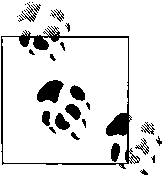
\includegraphics[width=2cm,clip]{paipai.png}
\end{wrapfigure}
\mbox{}\begin{flushleft}本节讨论常用的非实时进程,实时进程需要不同的调度标准和独立的优先级系统,留到以后讨论。\end{flushleft}

Linux不是随意地进行进程调度。进程都有一个影响他们何时运行,运行多久的优先级。历史上,Unix把这个优先级称为“nice values”,因为低优先级的进程往往允许其他进程分享更多的处理器时间,也就意味着该进程对系统的其他进程更加友好。

``nice value"是在进程运行的时候指定的,Linux调度器基于这样的原则来调度:高优先级的程序总是先运行。同时,nice值也指明了进程的时间片长度。

合法的优先级在-20到19之间,默认为0。有些让人疑惑的是,nice值越低,优先级越高,时间片越长;相反,nice值越高,优先级越低,时间片越短,增加一个进程的nice值意味着该进程对系统更友好。数字令人容易混淆。当我们说一个进程有高优先级的时候,我们认为该进程应该更快地开始运行,运行更长的时间,显然对系统的友好度更低。

\subsection{nice()}

Linux提供了获取和设置进程nice值的系统调用,最简单的就是nice():

\begin{lstlisting}
  #include <unistd.h>
  int nice (int inc);
\end{lstlisting}

成功调用nice()将在现有优先级上增加inc,并返回新值。只有拥有CAP\_SYS\_NICE能力(实际上,就是root所有的进程)才能够使用负值inc,减少友好度,增加优先级。因此,非root进程只能降低优先级(增加nice值)。

遇到错误,nice()返回-1,但是-1也可能是成功时的返回值,因此为了区别成功与否,在调用前应该对errno置0,调用后检查。举例来说:

\begin{lstlisting}
  int ret;
  errno = 0;
  ret = nice (10);  /* increase our nice by 10 */
  if (ret == -1 && errno !=0)
    perror ("nice");
  else
    printf ("nice value is now %d\n", ret);
\end{lstlisting}

对于nice(),Linux只会返回一种错误号: EPERM,表明进程试图提高优先级而又没有CAP\_SYS\_NICE能力。其他的系统还会在nice值超出范围的时候返回 EINVAL,而Linux会把非法的值放到对应的边界上。

传递参数0给nice()是获得当前优先级的简单方法:

\begin{lstlisting}
  printf("nice value is currently %d\n", nice (0));
\end{lstlisting}

通常,进程需要设定绝对的优先级而不是相对增量的时候,可以用下边的代码:

\begin{lstlisting}
  int ret, val;
  /* get current nice value */
  val = nice (0);
  /* we want a nice value of 10 */
  val = 10 - val;
  errno = 0;
  ret = nice (val);
  if (ret == -1 && errno != 0)
    perror ("nice");
  else
    printf ("nice value is now %d\n", ret);
\end{lstlisting}

\subsection{getpriority()和setpriority()}

更好的解决方案是用getpriority()和setpriority()系统调用,可以带来更多的控制能力,当然使用起来也更为复杂:

\begin{lstlisting}
  #include <sys/time.h>
  #include <sys/resource.h>
  int getpriority (int which, int who);
  int setpriority (int which, int who, int prio);
\end{lstlisting}

两个函数作用于``which"和``who"指定的进程,进程组或者用户,其中“which“的取值为 PRIO\_PROCESS、 PRIO\_PGRP 或者 PRIO\_USER,对应地,“who”就说明了进程ID,进程组ID或者用户ID。当“who”是0的时候,分别是当前进程,当前进程组或者当前用户。

getpriority()返回指定进程中的最高优先级(nice值最小),setpriority()则将所有进程的优先级都设为“prio“。同nice()一样,只有拥有CAP\_SYS\_NICE能力的进程能够提高一个进程的优先级(降低nice值),更进一步地说,只有这样的进程才能够调整不属于当前用户的进程的优先级。

getpriority()遇到错误的时候返回-1,但-1也可能是成功的返回值,因此同nice()一样,为了处理错误情况,程序员必须在调用前清空error值。setpriority()就不必如此,它总是成功返回0,错误返回-1。

下面是得到当前进程优先级的例子:

\begin{lstlisting}
  int ret;
  ret = getpriority (PRIO_PROCESS, 0);
  printf ("nice value is %d\n", ret);
\end{lstlisting}

设置当前进程组所有进程优先级为10的例子:

\begin{lstlisting}
  int ret;
  ret = setpriority (PGIO_PGRP, 0, 10);
  if (ret == -1)
    perror ("setpriority");
\end{lstlisting}

错误的时候,函数会设置errno为以下几个值:

\begin{eqlist*}
\item[EACCESS] 进程没有CAP\_SYS\_NICE能力,却企图提高进程优先级。(仅适用于setpriority())
\item[EINVAL] ``which"的值不在PRIO\_PROCESS, PRIO\_PGRP或PRIO\_USER之中。
\item[EPERM] 指定的进程有效用户ID和调用进程有效用户ID不一致,且调用进程没有CAP\_SYS\_NICE能力。(仅适用于setpriority())
\item[ESRCH] 不存在符合“which”和“who”的进程。
\end{eqlist*}

\subsection{I/O优先级}

作为进程优先级的补充,Linux还允许进程指定I/O优先级,内核I/O调度器(参考第四章)总是优先响应来自于高I/O优先级的请求。

缺省情况下,I/O调度器用进程友好度决定I/O优先级,因此,设置优先级自动改变I/O优先级。然而,Linux内核还有两个系统调用来单独获取和设置I/O:

\begin{lstlisting}
  int ioprio_get (int which, int who)
  int ioprio_set (int which, int who, int ioprio)
\end{lstlisting}

不幸地是,内核没有导出这两个系统调用,glibc也没有提供用户空间接口。没有glibc的支持,函数用起来是相当麻烦的。以后,如果未来glibc开始支持的时候,接口有可能和系统调用不同。在这之前,有两个可移植方法来操作进程I/O优先级:通过nice值,或者类似于``ionice"\footnote[1]{ionice是util-linux包的一部分,可以从http://www.kernel.org/pub/linux/utils/utl-linux得到,以GNU General Public License v2授权}的实用程序。

不是所有的I/O调度器都支持I/O优先级,特别地,Complete Fair Queuing(CFQ) I/O调度器支持,其他的标准调度器不支持。如果I/O调度器不支持I/O优先级,相关系统调用被忽略而没有任何提示信息。

\section{处理器亲和度}

Linux可以在一个系统中使用多处理器,除了启动进程,支持多处理器的大多数工作都依赖于进程调度器。在对称多处理机(SMP)上,进程调度器必须决定每个CPU上运行哪个进程,因此,必须解决两个问题:调度器必须充分利用系统的处理器,尽量避免处理器空闲。然而,如果一个进程曾在某一CPU上运行,进程调度器还应该尽量把它放在同一CPU上,因为处理器间的进程迁移会带来性能损失。

最大的性能损失来自于迁移带来的缓存效应\footnote[2]{译者注:cache effects}。现代SMP系统的设计中,每个处理器的缓存是各自独立的,也就是说,处理器并不共享缓存中的数据。因此,当进程迁移到新处理器上后写入新数据到内存时,原有处理器的缓存就过期了,这可能带来冲突。为了避免这种情况,缓存读入新的一块内存数据时标记其他缓存无效。因此,在任意时刻,任意数据仅在一个处理器的缓存中有效(假设该数据被缓存)。当进程迁移的时候,就有两方面的相关损失:进程不再能访问缓存数据且原有缓存中的数据必须标记为无效。考虑到这些损失,进程调度器应该尽量让进程停留在一个处理器。

实际上,进程调度器的两个目标有潜在的冲突。如果一个处理器比其他处理器有大得多的进程负载---或者更糟一些,一个处理器繁忙,其他处理器空闲---重新调度进程到低负载CPU上就是有意义的。决定何时移动进程来避免不平衡,称为负载均衡,对SMP机器的性能至关重要。

处理器亲和度表明一个进程停留在同一处理器上的可能性。术语“软亲和度”(soft affinity)表明调度器持续调度进程到同一处理器上的自然倾向,从上文的讨论可以看到,这是非常有价值的特性。Linux调度器尽可能地这样做,只有当负载极端不平衡的时候,才考虑迁移进程;从而,最小化迁移的缓存效应,还能保证系统中的处理器负载基本平衡。

然而有些时候,用户或者应用程序需要保证进程和处理器间的绑定,这通常发生在进程非常依赖缓存\footnote[3]{译者注: cache-sensitive},期望停留在同一处理器的情况下。术语“硬亲和度”(hard affinity)描述了强制内核保证进程到处理器的绑定。

\subsection{sched\_getaffinity() 和 sched\_setaffinity()}

进程从父进程继承处理器亲和度;在默认情况下,可能运行在任何CPU上。Linux提供两个系统调用来获取和设定进程的硬亲和度\footnote[3]{译者注: hard affinity}:

\begin{lstlisting}
  #define _GNU_SOURCE
  #include <sched.h>
  typedef struct cpu_set_t;
  size_t CPU_SETSIZE;
  void CPU_SET (unsigned long cpu, cpu_set_t *set);
  void CPU_CLR (unsigned long cpu, cpu_set_t *set);
  int CPU_ISSET (unsigned long cpu, cpu_set_t *set);
  void CPU_ZERO (cpu_set_t *set);
  int sched_setaffinity (pid_t pid, size_t setsize, const cpu_set_t *set);
  int sched_getaffinity (pid_t pid, size_t setsize, const cpu_set_t *set);
\end{lstlisting}

调用sched\_getaffinity()可以获得由``pid"指定的进程的处理器亲和度,存储在cpu\_set\_t类型中,可以用特殊的宏访问。如果“pid”是0,则得到当前进程的亲和度。“setsize”参数是cpu\_set\_t的大小,glibc用它来保证将来类型变化时依然具有兼容性。成功的时候,函数返回0;错误返回-1,并设置errno。例子如下:

\begin{lstlisting}
  cpu_set_t set;
  int ret, i;
  CPU_ZERO (&set);
  ret = sched_getaffinity (0, sizeof (cpu_set_t), &set);
  if (ret == -1)
  perror ("sched_getaffinity");
  for (i = 0; i< CPU_SETSIZE; i++) {
    int cpu;
    cpu = CPU_ISSET (i, &set);
    printf ("cpu=%i is %s\n", i, cpu ? "set" : "unset" );
  }
\end{lstlisting}

在调用前,我们用CPU\_ZERO清零所有的二进制位,然后开始从0到CPU\_SETSIZE在set上的迭代。注意,CPU\_SETSIZE并不是set的大小---显然不能用它表示setsize---而是set可能表示的处理器数量。因为现在的实现用1个二进制位表示一个处理器,所以CPU\_SETSIZE比sizeof(cpu\_set\_t)大得多。我们用CPU\_ISSET检查系统中的处理器是否被绑定到这个进程,0表示否,非0则已经绑定。

只有实际存在的处理器才能被绑定,因此,在两个处理器的系统上运行上述代码将得到如下结果:

\begin{verbatim}
  cpu=0 is set
  cpu=1 is set
  cpu=2 is unset
  cpu=3 is unset
  ...
  cpu=1023 is unset
\end{verbatim}

从输出中可以看到,当前的CPU\_SETSIZE(从0开始)是1,024。

我们考虑CPU \#0和\#1这两个仅存的处理器,也许我们期望保证我们的进程仅仅运行在CPU \#0上。代码如下:

\begin{lstlisting}
  cpu_set_t set;
  int ret, i;
  CPU_ZERO (&set);        /* clear all CPUs */
  CPU_SET (0, &set);      /* allow CPU #0 */
  CPU_CLR (1, &set);      /* forbid CPU #1 */
  ret = sched_setaffinity (0, sizeof (cpu_set_t), &set);
  if (ret == -1)
    perror ("sched_setaffinity");
  for (i = 0; i < CPU_SETSIZE; i++) {
    int cpu;
    cpu = CPU_ISSET (i, &set);
    printf ("cpu=%i is %s\n", i, cpu ? "set" : "unset");
  }
\end{lstlisting}

  我们首先总是用CPU\_ZERO清零set,然后用CPU\_SET对CPU \#0置1, 用CPU\_CLR对CPU \#1置0。已经清零了整个set,所以CPU\_CLR清零是多余的,仅仅是处于完整性的考虑。

  在同样的两处理器系统上运行,得到了稍微不同的输出:

\begin{verbatim}
  cpu=0 is set
  cpu=1 is unset
  cpu=2 is unset
  ...
  cpu=1023 is unset
\end{verbatim}

  现在CPU \#1被禁止,该进程无论如何总是运行在CPU \#0上。

  可能的四种错误号如下:

\begin{eqlist*}
\item[EFAULT] 提供的指针在进程的地址空间外或者无效。
\item[EINVAL] 系统中没有处理器被允许调度(仅适用于sched\_setaffinity()),或者setsize小于内核中表示处理器集合的数据结构的大小。
\item[EPERM] pid指明的进程不属于调用进程的有效用户ID,而且该进程没有CAP\_SYS\_NICE能力。
\item[ESRCH] pid指定的进程不存在。
\end{eqlist*}

\section{实时系统}

  在计算机领域,术语“实时”往往是混乱和误解的根源。如果一个系统受到操作期限\footnote[1]{译者注: operational deadlines}---请求和响应之间的最小量和命令次数---的支配,就称该系统是“实时”的。几乎在所有汽车上都可以看到的“防抱死(ABS)“系统就是一个类似的实时系统。在这个系统中,当踩下刹车的时候,计算机通过一秒内多次施加和释放最大刹车压力来调节刹车压力,以防止轮胎“锁死”,保证刹车性能,避免汽车失控。而系统的操作期限就是系统能够多快地相应轮胎“锁死”,能够多快地施加刹车压力。

  包括Linux在内的多数现代操作系统都提供了某些层次的实时支持。

\subsection{软硬实时系统}

  实时系统分为软硬实时系统两大类。硬实时系统对于操作期限要求非常严格,超过期限就会产生失败,后果很严重。另一方面,软实时系统却不认为超过期限是一个严重的失败。

  硬实时系统很容易分辨:防抱死系统、军用武器系统、医疗设备、信号处理都是比较典型的例子。软实时系统则不太容易分辨,一个比较明显的例子是视频处理程序: 如果超过了操作时限,用户会注意到一些质量下降,但是少量的丢帧还是可以忍受的。

  很多应用都有强制的时间要求,如果不能满足要求就会损害用户体验,多媒体应用,游戏和网络程序都在其中。文字编辑器怎么样呢?如果程序不能很快地响应键盘输入,体验就很差,用户会感到愤怒或者有很深的挫败感。它是软实时应用吗?当然,当开发者写程序的时候,他们意识到必须及时地响应输入。但它构成一个强制的操作期限吗?软实时程序的定义说得很清楚。

  和一般看法不同,实时系统并不一定快。实际上,在相同的硬件条件下,实时系统更可能慢于非实时系统,原因在于,即使不考虑其他因素,支持实时进程也会增加系统的负担。类似的,软硬实时系统的区分也不等同于操作时限的长短。在检测到过量的中子流出的几秒钟内,如果SCRAM系统不把控制杆放低一些的话,核反应堆就可能过热。这就是一个有漫长操作期限的硬实时系统。相反地,如果一个视频播放器不能够在100ms内填充回放缓冲区,就会跳过一些帧或者发出结结巴巴的声音,这是一个对操作期限要求较高的软实时系统。

\subsection{延时,抖动和截止期限}

  延时指刺激发生直到响应运行的时间,如果延时小于等于操作期限,系统运行正常。在很多硬实时系统中,操作期限和延时是等价的,系统以固定的间隔在确定时刻处理请求。在软实时系统中,响应不需要那么精确,延时也会出现一些变化,响应只需要在截止期限内发生就行。

  通常很难测量延时,因为测量它必须知道刺激发生的时间。然而,给请求打上时间戳,往往影响及时响应的能力。因此,一般的测量延迟的方法都不这么处理;实际上,人们测量成功响应时间的变化。连续事件中间的时间变化称之为抖动,而不测量延时。

  举例来说,考虑每10ms一次的刺激。为了测量系统性能,我们给响应打上时间戳,确保每10ms响应一次,几次测量之间的偏差就是抖动,我们所测量的就是连续响应间的变化。不知道请求发生的时间,我们也就不知道请求和响应之间的时间差;即使知道请求每10ms一次,我们也不知道第一次请求何时开始。或许更令人惊讶的是,很多测量延时的尝试都搞错了,实际得到了抖动而不是延时。可以肯定的是,抖动是一个有用的测量值,如此的测量也是非常有用的。无论如何,我们必须面对现实!

  硬实时系统经常出现一些非常小的抖动,因为他们在一段时间后而不是那段时间内响应刺激。系统追求零抖动,从而使延时等于操作间隔。如果延时超过间隔,就会失败。

  软实时系统对抖动更宽容。在这些系统中,理想情况下响应时间会在操作间隔内,通常快一些,有时慢一点。因此,抖动就可以完美地替代延时作为性能测量的目标了。

\subsection{Linux的实时支持}

  Linux通过IEEE Std 1003.1b-1993(缩写为POSIX 1993或POSIX.1b)定义的一系列系统调用来为应用程序提供软实时支持。

  技术上讲,POSIX标准并没有说明它提供的实时支持是软还是硬。实际上,POSIX标准仅仅描述了一些基于优先级的调度策略,操作系统服从何种时间约束取决于操作系统设计者。

  过去这些年,Linux内核在不牺牲性能的情况下,取得了越来越好的实时支持,提供越来越小的延时和更加一致的抖动。主要原因在于改进能够帮助很多类应用程序,比如桌面和I/O约束进程,而不仅仅是实时应用;改进对于Linux在嵌入式和实时领域的成功也有很大贡献。

  不幸的是,许多嵌入式和实时领域对Linux内核的修改仅仅存在于定制的Linux解决方案中,独立于主流的官方内核。其中的一些修改进一步减少延时,甚至达到硬实时系统的标准。下面的几节仅仅讨论官方内核接口和主流内核行为。幸运的是,大多数实时修改都利用POSIX接口,因此,接下来的讨论也适用于修改版系统。

\subsection{Linux调度策略和优先级}

  linux对进程的调度行为依赖于进程的调度策略,也称之为调度类别。Linux提供了两类实时调度策略作为正常默认策略的补充。头文件<sched.h>中的预定义宏表示各个策略:分别为SCHED\_FIFO, SCHED\_RR和SCHED\_OTHER。

  每一个进程都有一个与nice值无关的静态优先级,对于普通程序,值为0;对于实时程序,它为1到99。Linux调度器始终选择最高优先级的进程运行(静态优先级数值最大的进程)。如果一个优先级为50的进程在运行,此时一个优先级为51的进程就绪,调度器会直接抢占当前进程,转而运行新到的高优先级进程。相反,如果一个优先级为49的进程就绪,它会一直等待直到优先级为50的进程阻塞才可运行。因为普通进程优先级为0,所以实时进程总会抢占非实时进程开始运行。

\subsubsection{“先进先出”策略}

  先进先出(FIFO)策略是没有时间片的非常简单的实时策略。只要没有高优先级进程就绪,FIFO类型进程就会持续运行,用宏SCHED\_FIFO表示。

  因为缺少时间片,它的操作策略相当简单:

\begin{itemize}
\item \begin{flushleft}一个就绪的FIFO型进程如果是系统中的最高优先级进程就会一直保持运行。特别的,一旦FIFO类进程就绪,它就会直接抢占普通进程。\end{flushleft}
\item \begin{flushleft}FIFO型进程持续运行直到阻塞或者调用sched\_yield(),或者高优先级进程就绪。\end{flushleft}
\item \begin{flushleft}当FIFO型进程阻塞时,调度器将其移出就绪队列。当它恢复时,被插到相同优先级进程队列的末尾。因此,它必须等待高优先级或同等优先级进程停止运行。\end{flushleft}
\item \begin{flushleft}当FIFO型进程调用sched\_yield()时,调度器将其放到同等优先级队列的末尾,因此,它必须等待其他同等优先级进程停止运行。如果没有其他同等优先级进程,sched\_yield()将没有作用。\end{flushleft}
\item \begin{flushleft}当FIFO型进程被抢占,它在优先级队列中的位置不变。因此,一旦高优先级进程停止运行,被抢占的FIFO型进程就会继续运行。\end{flushleft}
\item \begin{flushleft}当一个进程变为FIFO型或者进程静态优先级改变,它将会被放到相应优先级队列的头部。因此,新来的FIFO型进程能够抢占同等优先级进程。\end{flushleft}
\end{itemize}

  本质上,我们可以认为FIFO型进程只要具有最高优先级,就能一直运行。比较有趣的部分在于同等优先级的FIFO进程之间的关系。

\subsubsection{轮转策略}

  轮转策略类似于FIFO类型,仅仅引入了处理同等优先级进程的附加规则,以SCHED\_RR表示。

  调度器给每一个RR型进程分配一个时间片。当RR型进程耗光时间片时,调度器将其放到所在优先级队列的末尾;通过这种方式,RR型进程间就能轮转调度。如果只有一个进程在给定优先级上,RR型就等同于FIFO型,这种情况下,它耗尽时间片,然后直接继续运行。

  我们可以认为RR型进程等同于FIFO型进程,仅仅是在时间片耗尽的时候停止运行,排到同等优先级队列的末尾。

  选择SCHED\_FIFO或者SCHED\_RR仅仅取决于优先级内部的操作,RR型的时间片仅在相同优先级的进程间相关。FIFO进程会不停运行,RR型进程会在给定优先级进程间调度,但是都不会出现高优先级进程等待低优先级进程的情况。

\subsubsection{普通调度策略}

  SCHED\_OTHER代表标准调度策略,适用于默认的非实时进程。所有这些进程的静态优先级都为0,因此,任意就绪FIFO或RR型进程都会抢占他们。

  调度器利用先前讨论过的nice值来划分普通进程的优先级,静态优先级不受nice值的影响,始终为0。

\subsubsection{批调度策略}

  SCHED\_BATCH是批调度或空闲调度的策略,它在某种程度上是实时调度的对立面:这种类型的进程只在系统中没有其他就绪进程时才会运行,即使那些进程已经耗光时间片。这不同于低优先级进程,在那种情况下,进程最终会在高优先级进程耗光时间片后开始运行。

\subsubsection{设置Linux调度策略}

  进程可以通过sched\_getscheduler()和sched\_setscheduler()来操作Linux调度策略:

\begin{lstlisting}
  #include <sched.h>
  struct sched_param {
    /* ... */
    int sched_priority;
    /* ... */
  };
  int sched_getscheduler (pid_t pid);
  int sched_setscheduler (pid_t pid, int policy, const struct sched_param *sp);
\end{lstlisting}

  对sched\_getscheduler()的成功调用将返回由pid指定进程的调度策略,如果pid为0,则返回调用进程的调度策略。<sched.h>中定义了一个整数表示调度策略:SCHED\_FIFO表示先进先出策略,SCHED\_RR表示轮转策略,SCHED\_OTHER表示普通进程。遇到错误,函数返回-1(-1不是有效的调度策略),同时适当地设置错误号。

  用法很简单:

\begin{lstlisting}
  int policy;
  /* get out scheduling policy */
  policy = sched_getscheduler (0);
  switch (policy) {
    case SCHED_OTHER:
      printf ("Policy is normal\n");
      break;
    case SCHED_RR:
      printf ("Policy is round-robin\n");
      break;
    case SCHED_FIFO:
      printf ("Policy is fist-in, first-out\n");
      break;
    case -1:
      perror ("sched_getscheduler");
      break;
    default:
      fprintf (stderr, "Unknown policy!\n");
  }
\end{lstlisting}

  调用sched\_setscheduler()将设置由pid指定进程的调度策略,与策略有关的其他参数则由sp确定。当pid是0时,进程将设置自己的策略和参数。函数成功返回0,失败返回-1并设置错误号。

  sched\_param结构体中的有效字段依赖于操作系统支持的调度策略。SCHED\_RR和SCHED\_FIFO都至少需要一个字段sched\_priority来指明静态优先级。SCHED\_OTHER不使用任何字段,虽然未来的调度策略可能会用到。因此,可移植和合法的程序不应该对结构的布局作出任何假设。

  设置进程调度策略和参数很简单:

\begin{lstlisting}
  struct sched_param sp = { .sched_priority = 1 };
  int ret;
  ret = sched_setscheduler (0, SCHED_RR, &sp);
  if (ret == -1) {
    perror ("sched_setscheduler");
    return 1;
  }
\end{lstlisting}

  代码设置调用进程采用轮转调度策略,优先级为1。我们假设1是有效优先级值---技术上讲,并不必要。我们会在下一节讨论如何得到有效优先级取值范围。

  设置除SCHED\_OTHER外的调度策略都需要CAP\_SYS\_NICE能力,因此,通常由root用户运行实时进程。从2.6.12内核开始,RLIMIT\_RTPRIO资源限制允许非root用户在一定上限内设置实时优先级。

  错误码。错误时设置四种错误值:

\begin{eqlist*}
\item[EFAULT] 指针sp指向的内存区域非法或不可访问。
\item[EINVAL] policy指定的调度策略无效,或者sp值不适用于给定的策略(仅实用于sched\_setscheduler())。
\item[EPERM] 调用进程不具备必要的能力。
\item[ESRCH] pid指定的进程不在运行状态。
\end{eqlist*}

\subsection{设置调度参数}

  POSIX定义的sched\_getparam()和sched\_setparam()接口可以获取和设置已有调度策略的相关参数:

\begin{lstlisting}
  #include <sched.h>
  struct sched_param {
    /* ... */
    int sched_priority;
    /* ... */
  };
  int sched_getparam (pid_t pid, struct sched_param *sp);
  int sched_setparam (pid_t pid, const struct sched_param *sp);
\end{lstlisting}

  sched\_getscheduler()接口仅仅返回调度策略,sched\_getparam()则将pid进程的调度参数存储在sp中:

\begin{lstlisting}
  struct sched_param sp;
  int ret;
  ret = sched_getparam (0, &sp);
  if (ret == -1) {
    perror ("sched_getparam");
    return 1;
  }
  printf ("Our priority is %d\n", sp.sched_priority);
\end{lstlisting}

  pid为0,返回调用进程的参数。成功返回0,错误返回-1,设置错误号。

  因为sched\_setscheduler()也能设置任何调度参数,所以sched\_setparam()仅仅用来稍后修改参数:

\begin{lstlisting}
  struct sched_param sp;
  int ret;
  sp.sched_priority = 1;
  ret = sched_setparam (0, &sp);
  if (ret == -1) {
    perror ("sched_setparam");
    return 1;
  }
\end{lstlisting}

  函数成功则根据sp设置pid指定进程的调度参数,返回0。失败,返回-1,设置errno。

  如果我们顺序运行上文两段代码,应该会看到这样的输出:

\begin{verbatim}
  Our priority is 1
\end{verbatim}

  这个例子再一次假设1是合法值,此时它确实是,但可移植的程序应该主动去确定这一点。稍后我们会看看如何检测有效优先级的范围。

\subsubsection{错误码}

  函数可能设置四种错误码:

\begin{eqlist*}
\item[EFAULT] 指针sp指向的内存区域非法或不可访问。
\item[EINVAL] sp值不适用于给定的策略(仅实用于sched\_getparam())。
\item[EPERM] 调用进程不具备必要的能力。
\item[ESRCH] pid指定的进程不在运行状态。
\end{eqlist*}

\subsubsection{确定有效优先级的范围}

  在上边的例子中,我们把优先级数值硬编码到函数调用中。POSIX并不能保证系统上确定的调度优先级可用,仅仅要求至少有32阶优先级。在“Linux调度策略和优先级”一节中我们曾提到Linux为两类实时调度策略提供了1到99阶共99级。一个清晰可移植的程序通常实现自己的优先级范围,然后映射到操作系统的范围上。比如,你需要四个不同的实时优先级层次,你可以动态地确定优先级范围再从中选择四个。

  Linux提供两个系统调用来获得优先级范围,一个返回最小值,另一个返回最大值:

\begin{lstlisting}
  #include <sched.h>
  int sched_get_priority_min (int policy);
  int sched_get_priority_max (int policy);
\end{lstlisting}

  一旦成功执行,sched\_get\_priority\_min()返回最小值,sched\_get\_priority\_max()返回policy所关联策略的最大有效优先级。两个函数调用成功都返回0(此处为原文错误,正常应该返回对应的值),调用失败返回-1, 唯一可能的错误是policy值非法,此时错误号被设置为 EINVAL。

  用法很简单:

\begin{lstlisting}
  int min, max;
  min = sched_get_priority_min (SCHED_RR);
  if (min == -1) {
    perror ("sched_get_priority_min");
    return 1;
  }
  max = sched_get_priority_max (SCHED_RR);
  if (max == -1) {
    perror ("sched_get_priority_max");
    return 1;
  }
  printf ("SCHED_RR priority range is %d - %d\n", min, max);
\end{lstlisting}

  在标准Linux系统上,代码运行得到:

\begin{verbatim}
  SCHED_RR priority range is 1 - 99
\end{verbatim}

  此前讨论过,数值越大就意味着越高的优先级。下边的代码可以设置进程的相应策略的最高优先级:

\begin{lstlisting}
  /*
  * set_highest_priority – set the associated pid's scheduling
  * priority to the highest value allowed by its current
  * scheduling policy. If pid is zero, sets the current
  * process's priority.
  *
  * Returns zero on success.
  */
  int set_highest_priority (pid_t pid)
  {
    struct sched_param sp;
    int policy, max, ret;
    policy = sched_getscheduler (pid);
    if (policy == -1)
      return -1;
    max = sched_get_priority_max (policy);
    if (max == -1)
      return -1;
    memset (&sp, 0, sizeof (struct sched_param));
    sp.sched_priority = max;
    ret = sched_setparam (pid, &sp);
    return ret;
  }
\end{lstlisting}

  程序一般都是获得系统的最小或最大值,然后按1递增(比如max-1, max-2等等),分配给指定的进程。

\subsection{sched\_rr\_get\_interval()}

  前边说过,SCHED\_RR进程除了拥有时间片外和SCHED\_FIFO进程相同。当SCHED\_RR进程耗光时间片的时候,调度器将其放到同一优先级队列的末尾。通过这种方式,所有相同优先级的SCHED\_RR进程循环运行。无论运行进程是否还有时间片,高优先级进程(包括同等或较高优先级的SCHED\_FIFO进程)总是会抢占它。

  POSIX定义了获得进程时间片长度的接口:

\begin{lstlisting}
  #include <sched.h>
  struct timespec {
    time_t tv_sec;    /* seconds */
    long   tv_nsec;   /* nanoseconds */
  };
  int sched_rr_get_interval (pid_t pid, struct timespec *tp);
\end{lstlisting}

  sched\_rr\_get\_interval()这个糟糕命名的函数,对它的成功调用将把pid指定进程的时间片存储在tp指向的timespec结构中,然后返回0;失败,函数返回-1,设置errno。

  POSIX规定这个函数只能工作于SCHED\_RR进程,然而在Linux上它可以获得任意进程的时间片长度。可移植应用必须假定函数仅能工作于轮转策略,面向Linux的程序可以作一些必要的拓展。例子如下:

\begin{lstlisting}
  struct timespec tp;
  int ret;
  /* get the current task's timeslice length */
  ret = sched_rr_get_interval (0, &tp);
  if (ret == -1) {
    perror ("sched_rr_get_interval");
    return 1;
  }
  /* convert the seconds and nanoseconds to milliseconds */
  printf ("Our time quantum is %.2lf milliseconds\n",
  (tp.tv_sec * 1000.0f) + (tp.tv_nsec / 1000000.0f));
\end{lstlisting}

  如果进程是FIFO类型,则tv\_sec和tv\_nsec都是0,意味着无限长的时间片。

\subsubsection{错误码}

  共有三种可能的错误码:

\begin{eqlist*}
\item[EFAULT] 指针tp指向的内存无效或者不可访问。
\item[EINVAL] pid无效(比如pid是负值)。
\item[ESRCH] pid有效,但指向不存在的进程。
\end{eqlist*}

\subsection{关于实时进程的一些提醒}

  因为实时进程的本质,开发者在开发和调试此类程序的时候应该特别慎重。如果一个实时程序仓促行事,系统可能失去响应。只要没有高优先级程序,实时程序中任何处理器约束的循环---或者是任何不会阻塞的代码---都会永远地运行下去。

  因此,设计实时程序需要小心和注意,这些有很高权限的程序很容易就使系统崩溃。下面是一些技巧和提醒:

\begin{itemize}
\item 切记任何处理器约束的循环,如果没有中断或者高优先级进程来打断它,在完成前都会一直运行。如果是无限循环,系统将失去响应。
\item 因为实时进程运行会占有系统的所有资源,所以在设计的时候需要特别注意,不要过度损害系统其他部分的处理器时间。
\item 小心忙等待。如果一个实时进程忙等待一个较低优先级进程占有的资源,该进程会永远处于忙等待状态。
\item 当开发实时程序的时候,永远开着一个终端,运行一个更高优先级的进程。在紧急情况下,终端会保持响应,允许你杀死失控的进程。(当终端空闲等待输入的时候,不会影响其他实时进程。)
\item util-linux工具包中的chrt实用程序可以使获取和设置实时进程属性更轻松。它可以简单地让任意程序运行在实时调度策略下,比如前述的终端,或者改变已有应用的实时优先级。
\end{itemize}

\subsection{确定性}

  实时进程乐于看到确定性。在实时计算中,如果给予相同的输入,一个动作总是在相同的时间内产生相同的结果,我们就说这个动作是确定的。现代计算机可以说是不确定的集合体:多级缓存(命中与否不可预测),多处理器,分页,交换,和多任务都使估计一个动作需要多长时间变得不可能。显然我们现在每一个动作(相对于硬盘访问)都是“不可思议的快”,但是同时现代系统也使得我们难于精确测量每一个动作的时间。

  实时应用一般会尽量限制不可预测性,和最坏情况下的延时。下面的章节讨论达到目标的两种方法。

\subsubsection{数据故障预测和内存锁定}

  想象一下:ICBM(译者注:洲际导弹系统)监视器接入产生硬件中断,设备驱动迅速地拷贝硬件数据到内核。驱动会注意到一个进程因等待数据阻塞在硬件设备上,因此会通知内核唤醒进程。内核注意到该进程是实时进程且拥有高优先级,就会直接抢占当前运行进程,将注意力转移过来,决定直接调度实时进程。调度器转换到运行实时进程,上下文切换到相应的地址空间。进程开始运行,整个过程需要0.3ms,在1ms的容忍限度内。

  现在考虑用户空间,实时进程注意到接入的ICBM,开始处理轨道。计算好弹道后,实时进程开始配置反导系统。仅仅花掉0.1ms,足够ABM响应和拯救生命。但是---不---ABM的代码已经被交换到硬盘上。于是发生页错误,处理器切回内核模式,启动硬盘I/O来获得交换出去的数据。实时进程会一直休眠直到处理完页错误,几秒钟过去了,一切太晚了。

  显然,分页和交换给实时进程带来了很多不确定性。为了阻止这种灾难,实时应用往往“通过锁定”或者“硬连接“来将地址空间中的页提前放入物理内存,阻止其被交换出去。一旦页被锁定,内核就不会将其交换出去,任何访问都不会引起页错误,大多数实时应用都锁定部分和全部页面到物理内存。

  Linux为两种方法都提供了接口。Chapter 4讨论了故障预测的接口,Chapter 8将讨论锁定内存的接口。

\subsubsection{CPU亲和度和实时进程}

  实时应用的第二个难点在于多任务。虽然Linux内核是抢占式的,但是调度器并不总能直接调度另一个进程。有时,当前进程运行在内核中的临界区,调度器就必须等待它退出临界区,如果此时有一个实时进程要运行,延时将不可接受,很快就会超出操作期限。

  因此,多任务和分页一样也带来了相似的不确定。对于多任务的解决方案也一样:消除它。当然,前提是你不能简单地消灭其他所有进程,如果你可以,你就不需要Linux了---简单定制的操作系统就能满足要求。如果你的系统中有多个处理器,可以指定一个或多个专门用于实时进程。从实际效果上讲,你把实时进程和多任务分离开来。

  本章已经讨论过操作进程CPU亲和度的系统调用。一个潜在的对实时进程的优化是为每一个实时进程保留一个处理器,剩下的处理器由其他进程共享。

  最简单的方法是修改Linux的init程序,SysVinit\footnote[1]{SysVinit源代码可以在ftp://ftp.cistron.nl/pub/people/miquels/sysvinit/取得,以GNU General Public License v2授权},从而可以在启动前做类似下面的动作:

\begin{lstlisting}
  cpu_set_t set;
  int ret;
  CPU_ZERO (&set); /* clear all CPUs */
  ret = sched_getaffinity (0, sizeof (cpu_set_t), &set);
  if (ret == -1) {
    perror ("sched_getaffinity");
    return 1;
  }
  CPU_CLR (1, &set); /* forbid CPU #1 */
  ret = sched_setaffinity (0, sizeof (cpu_set_t), &set);
  if (ret == -1) {
    perror ("sched_setaffinity");
    return 1;
  }
\end{lstlisting}

  代码首先得到初始的可用处理器集合,我们期望是全体处理器。然后移出一个处理器CPU \#1,更新可用处理器集合。

  因为可用处理器集合在父子进程间继承,init又是所有进程的祖先,所以所有的进程都会根据修改后的处理器集合运行,CPU \#1上将没有任何进程。

  接下来,修改实时程序让它仅在CPU \#1上运行:

\begin{lstlisting}
  cpu_set_t set;
  int ret;
  CPU_ZERO (&set); /* clear all CPUs */
  CPU_SET (1, &set); /* allow CPU #1 */
  ret = sched_setaffinity (0, sizeof (cpu_set_t), &set);
  if (ret == -1) {
    perror ("sched_setaffinity");
    return 1;
  }
\end{lstlisting}

  如此,结果就是实时进程仅运行在CPU \#1上,其他的所有进程分享其他处理器。

\section{资源限制}

  Linux内核有对进程的资源限制,明确规定了进程可以消耗的内核资源的上限,比如打开文件的数目,内存页数,未处理的信号等等。限制是强制性的,内核不会允许进程的超过这一硬性限制。比如,如果一个打开文件的操作会使得进程拥有的文件超出资源限制,open()调用会失败\footnote[2]{此时,调用会设置错误号为EMFILE,表明进程达到文件数量上限。Chapter 2讨论了open()系统调用}。

  Linux提供了两个操作资源限制的系统调用。两个都是POSIX的标准调用,Linux做了一些补充,分别用getlimit()和setlimit()获取和设置限制:

\begin{lstlisting}
  #include <sys/time.h>
  #include <sys/resource.h>
  struct rlimit {
    rlim_t rlim_cur; /* soft limit */
    rlim_t rlim_max; /* hard limit */
  };
  int getrlimit (int resource, struct rlimit *rlim);
  int setrlimit (int resource, const struct rlimit *rlim);
\end{lstlisting}

  一般用类似RLIMIT\_CPU的整数常量表示资源,rlimit结构表示实际限制。结构定义了两个上限:软限制和硬限制。内核对进程强制施行软限制,但进程自身可以修改软限制,可以是0到硬限制之间的任意值。不具备CAP\_SYS\_RESOURCE能力的进程(比如,非root进程),只能调低硬限制。非特权程序不能提升硬限制,包括恢复为之前的较高的值;因此,调低硬限制是不可逆的。特权进程则可以设置硬限制为任意合法值。

  限制的含义与资源相关。比如资源是RLIMIT\_FSIZE,就表示一个进程可以创建的最大文件长度,单位是字节。此时如果rlim\_cur是1024,则进程不可以创建大于1K的文件,也不能扩展文件至1k以上。

  所有的资源限制都有两个特殊值: 0和无限。前者表示禁止使用资源,例如RLIMIT\_CORE是0,则内核不会创建内存转储文件。相反,后者表示不存在对资源的限制。内核用特殊值RLIM\_INFINITY表示无限,碰巧是-1,(可能和函数调用错误返回-1相混淆)。如果RLIMIT\_CORE是无限,则内核可以创建任意大小的内存转储文件。

  函数getrlimit()会在指针rlim指向的结构中放入resource的软硬限制。成功,返回0;错误,返回-1,设置错误号。

  相对的,函数setrlimit()按rlim指定的值设置resource的软硬限制。成功,返回0,内核更新对应的资源限制;失败,返回-1,设置错误号。

\subsection{限制列表}

  目前Linux提供了15种资源限制:


\begin{itemize}{}
\item RLIMIT\_AS\\
  进程地址空间上限,单位是字节。试图增加地址空间大小超过限制---比如调用mmap()和brk()函数---都会失败,返回ENOMEM。如果进程的栈自动增加,超过了限制,内核将给进程SIGSEGV信号。该限制的值通常为RLIM\_INFINITY。
\item RLIMIT\_CORE\\
  内存转储文件大小的最大值,单位是字节。如果非0,超出限制的内存转储文件将截短为最大限制大小;如果是0,将不会产生此类文件。
\item RLIMIT\_CPU\\
  一个进程可以使用的最长CPU时间,单位是秒。如果进程运行时间超出限制,将接受和处理内核发出的SIGXCPU信号。一个可移植程序必须在接收到该信号时中断,当POSIX没有定义内核的下一步动作。一些系统会中断进程,然而Linux允许进程继续运行,并且每秒发送给该进程一个SIGXCPU信号。一旦进程达到硬限制,将会收到SIGKILL信号并被中断。
\item RLIMIT\_DATA\\
  进程数据段和堆的大小,单位是字节。试图通过brk()来扩大数据段以超出限制将失败并返回ENOMEM。
\item RLIMIT\_FSIZE\\
  文件可以创建的最大文件,单位是字节。如果进程扩展文件超出了限制,内核将发送SIGXFSZ信号。默认情况下,信号将终止进程。但是,进程也可以在系统调用失败返回EFBIG时选择自己捕捉和处理信号。
\item RLIMIT\_LOCKS\\
  进程可以拥有的文件锁的最大数量(参见第七章关于文件锁的讨论)。一旦达到最大值,任何试图获取额外锁的努力都会失败,返回ENOLCK。Linux 2.4.25内核移除了这一功能,在当前内核中,可以设定这一限制,但不会起任何作用。
\item RLIMIT\_MEMLOCK\\
  不具有CAP\_SYS\_IPC能力的进程(非root进程)通过mlock(),mlockall()或者shmctl()能锁定的最多内存的字节数。当超过限制的时候,调用失败范围EPERM。实际上,实际限制向下舍入到整数个内存页。拥有CAP\_SYS\_IPC能力的进程可以锁定任意数量的内存页,此限制不再有效。在2.6.9内核前,该限制作由于有CAP\_SYS\_IPC能力的进程,非特权进程根本不能锁定内存页。此限制不属于POSIX标准,BSD首先引入了它。
\item RLIMIT\_MSGQUEUE\\
  用户可以在POSIX消息队列中分配的最多字节。如果新建的消息超出限制,mp\_open()函数失败返回ENOMEM。它不属于POSIX标准,于2.6.8内核中引入并为Linux独有。
\item RLIMIT\_NICE\\
  进程可以降底nice值(提升优先级)的最大值。本章前文已说明,普通进程只能提高友好度(降低优先级)。这个限制允许管理员规定进程可以合法地提升优先级的级数。因为nice值可能是负值,内核用$20-rlim\_cur$表示。因此,如果限制设置为40,进程友好度最低为-20(最高优先级)。2.6.12内核引入了这个限制。
\item RLIMIT\_NOFILE\\
  该值比进程可以打开的最多文件数大一。任何超出限制的企图都会失败返回EMFILE。在BSD中此限制名字为RLIMIT\_OFILE。
\item RLIMIT\_NPROC\\
  系统任意时刻允许的最多进程数。任何超出限制的企图都会失败,fork()返回EAGAIN。此限制不属于POSIX,由BSD引入。
\item RLIMIT\_RSS\\
  进程可以驻留在内存中的最多页数(即驻留集大小RSS)。仅在早期的2.4内核中强制执行;当前内核允许设置,但不强制执行。此限制不属于POSIX,由BSD引入。
\item RLIMIT\_RTPRIO\\
  没有CAP\_SYS\_NICE能力的进程可以拥有的最大实时优先级。通常,非特权进程不会要求实时调度。此限制不属于POSIX,由2.6.12内核引入并为Linux独有。
\item RLIMIT\_SIGPENDING\\
  用户消息队列中最多信号数。请求更多的信号将失败,sigqueue()这样的系统调用将返回EAGAIN。注意,可以无视这个限制而将一个尚未排入队列的信号实例加入该队列. 因此,总是可以向进程传递SIGKILL和SIGTERM信号。此限制不属于POSIX,由Linux独有。
\item RLIMIT\_STACK\\
  栈的最大字节长度。超出限制将收到SIGSEGV信号。
\end{itemize}

% 根据第一版的勘误,该段被全部替换。
%内核以用户为存储资源限制的基本单位,也就是说,相同用户的所有进程都会有相同的软硬资源限制,但是资源限制本身却描述了对单一进程的限制。比如,内核为每个用户都维护一个RLIMIT\_NOFILE,默认是1024,这个限制规定了每个进程能打开的最多文件数,而不是该用户总共能打开的文件数。还需要注意的是,这并不意味着限制能针对进程分别设置---一旦进程修改了RLIMIT\_NOFILE软限制,此用户的所有进程都会受到这种限制。

% 第二版中的该段翻译如下
内核中以进程为单位管理资源限制。子进程在fork的时候从父进程继承资源限制,限制通过exec进行维护。

\subsubsection{默认限制}

  默认限制取决于三个变量:初始软限制,初始硬限制和系统管理员。内核说明了初始软限制和初始硬限制,如表。内核在init进程中设置这些限制,并通过父子进程间的继承传递给所有的子孙进程。
\begin{center}
\begin{tabular}{ccc}
  \toprule [1pt]
  \rowcolor[gray]{.9}
    Resource limit & Soft limit & Hard limit\\
  \midrule
    RLIMIT\_AS & RLIM\_INFINITY & RLIM\_INFINITY\\
    RLIMIT\_CORE & 0 & RLIM\_INFINITY\\
    RLIMIT\_CPU & RLIM\_INFINITY & RLIM\_INFINITY\\
    RLIMIT\_DATA & RLIM\_INFINITY & RLIM\_INFINITY\\
    RLIMIT\_FSIZE & RLIM\_INFINITY & RLIM\_INFINITY\\
    RLIMIT\_LOCKS & RLIM\_INFINITY & RLIM\_INFINITY\\
    RLIMIT\_MEMLOCK & 8 pages & 8 pages\\
    RLIMIT\_MSGQUEUE & 800 KB & 800KB\\
    RLIMIT\_NICE & 0 & 0\\
    RLIMIT\_NOFILE & 1024 & 1024\\
    RLIMIT\_NPROC & 0 (implies no limit) & 0 (implies no limit)\\
    RLIMIT\_RSS & RLIM\_INFINITY & RLIM\_INFINITY\\
    RLIMIT\_RTPRIO & 0 & 0\\
    RLIMIT\_SIGPENDING & 0 & 0\\
    RLIMIT\_STACK & 8 MB & RLIM\_INFINITY\\
  \bottomrule[1pt]
\end{tabular}
\end{center}

  两种情况可以改变默认限制:

\begin{itemize}
\item 任何进程都可以在0到硬限制的范围内增加软限制,也可以减少硬限制,子进程可以通过fork来继承这些改变。
\item 特权进程可以任意设置硬限制,子进程同样可以通过fork来继承这些改变。
\end{itemize}

  普通进程继承体系中的root进程不太可能修改任何硬限制,因此,第一点更有可能是限制变化的原因。实际上,对于进程的限制往往由用户通过shell设定,系统管理员可以进行设置来提供种类繁多的限制。比如在Bourne-again shell(bash)中,管理员可以使用ulimit命令来设置。注意管理员不仅可以降低限制值,还可以提升软限制到硬限制,从而给用户提供更合理的限制。一般会使用RLIMIT\_STACK(在许多系统上该值都被设置为RLIM\_INFINITY)进行处理。

\subsection{获取和设置资源限制}

  解释了种种资源限制,让我们来考察一下获取和设置这些限制。获取限制很简单:

\begin{lstlisting}
  struct rlimit rlim;
  int ret;
  /* get the limit on core sizes */
  ret = getrlimit (RLIMIT_CORE, &rlim);
  if (ret == -1) {
    perror ("getrlimit");
    return 1;
  }
  printf ("RLIMIT_CORE limits: soft=%ld hard=%ld\n",
  rlim.rlim_cur, rlim.rlim_max);
\end{lstlisting}

  编译然后运行代码将得到:

\begin{verbatim}
  RLIMIT_CORE limits: soft=0 hard=-1
\end{verbatim}

  可以看到,软限制为0,硬限制为-1(-1代表无限)。因此我们可以设置软连接为任意值。下面的例子设置内存转储文件最大为32MB:
\begin{lstlisting}
  struct rlimit rlim;
  int ret;
  rlim.rlim_cur = 32 * 1024 * 1024; /* 32 MB */
  rlim.rlim_max = RLIM_INFINITY; /* leave it alone */
  ret = setrlimit (RLIMIT_CORE, &rlim);
  if (ret == -1) {
    perror ("setrlimit");
    return 1;
  }
\end{lstlisting}

\subsubsection{错误码}

  可能有三种错误代码:

\begin{eqlist*}
\item[EFAULT] rlim指向的内存非法或不可访问。
\item[EINVAL] resource的值非法,或者rlim.rlim\_cur的值大于rlim.rlim\_max(仅适用于setrlimit())。
\item[EPERM] 调用者没有CAP\_SYS\_RESOURCE能力却试图提升硬限制。
\end{eqlist*}

\ifx\atempxetex\usewhat
\XeTeXinputencoding "utf-8"
\fi
\defaultfont

\chapter{文件与目录管理}

在第2,3以及第4章中,我们给出了大量文件I/O的方法和系统调用。在本章,我们再次回到这个主题上来,但这次的重点不是文件读写,而是操作和管理文件及其元数据。

\section{文件及其元数据}

正如我们在第1章讨论的,每个文件均对应一个inode,它是由文件系统中唯一数值(被称为inode号)编址。inode既是位于类unix文件系统的物理对象,又是在Linux内核数据结构描述的概念实体。inode存储了与文件有关的元数据,例如文件的访问权限,最后访问时间,所有者,群组,大小以及文件数据的存储位置。 

你能使用ls命令的-i选项来获取一个文件inode编号:

\begin{tabular}{llll}
\$ ls -i & & &\\
1689459 Kconfig & 1689461 main.c & 1680144 process.c & 1689464 swsusp.c\\
1680137 Makefile & 1680141 pm.c & 1680145 smp.c & 1680149 user.c\\
1680138 console.c & 1689462 power.h & 1689463 snapshot.c & \\
1689460 disk.c & 1680143 poweroff.c & 1680147 swap.c & \\
\end{tabular}

该输出结果表示,例如文件disk.c的inode编号是1689460。在该文件系统中,不会有其他任何文件拥有该inode编号(inode number)。但在其他文件系统中,我们不能保证有同样的inode编号。 

\subsection{一组stat函数}

Unix提供了一组获取文件元数据的函数:

\begin{lstlisting}
  #include <sys/types.h>
  #include <sys/stat.h>
  #include <unistd.h>
  int stat (const char *path, struct stat *buf);
  int fstat (int fd, struct stat *buf);
  int lstat (const char *path, struct stat *buf);
\end{lstlisting}

这些函数均返回文件的信息。stat()返回由路径path参数指明的文件信息,而fstat()返回由文件描述符fd指向的文件信息。lstat()与stat()类似,但是对于符号链接,lstat()返回链接本身而非目标文件。

这些函数均在结构stat中存储了获取的文件信息。结构stat在<bits/stat.h>中定义,但真正的定义是包含在<sys/stat.h>中的:

\begin{lstlisting}
  struct stat {
    dev_t st_dev; /* ID of device containing file */
    ino_t st_ino; /* inode number */
    mode_t st_mode; /* permissions */
    nlink_t st_nlink; /* number of hard links */
    uid_t st_uid; /* user ID of owner */
    gid_t st_gid; /* group ID of owner */
    dev_t st_rdev; /* device ID (if special file) */
    off_t st_size; /* total size in bytes */
    blksize_t st_blksize; /* blocksize for filesystem I/O */
    blkcnt_t st_blocks; /* number of blocks allocated */
    time_t st_atime; /* last access time */
    time_t st_mtime; /* last modification time */
    time_t st_ctime; /* last status change time */
  };
\end{lstlisting}

下面是对结构体字段的详细解释:

\begin{itemize}
\item 字段st\_dev描述了文件位于什么设备节点上(我们在本章稍后将讨论设备节点)。如果文件不在本地设备上——例如,如果文件在网络文件系统(NFS)上—该值为0。
\item 字段st\_ino为文件的inode编号。
\item 字段st\_mode为文件的权限字段。第1章和第2章已讨论各权限位和权限的内容。
\item 字段st\_nlink为指向文件的硬链接数。每个文件至少有一个硬链接。
\item 字段st\_uid为文件所有者的用户ID。
\item 字段st\_gid为文件所属组ID。
\item 如果文件是设备节点,字段st\_rdev描述了该设备节点信息。
\item 字段st\_size提供文件字节数。
\item 字段st\_blksize为进行有效文件I/O的首选块大小。该值(或该值倍数)为用户缓冲I/O的最佳块大小(见第3章)。
\item 字段st\_blocks为分配给文件的块数目。当文件有洞时(也就是说该文件是一个稀疏文件)该值将小于st\_size值。
\item 字段st\_atime为最后文件访问时间。这是文件被访问的最近时间(例如,通过read()或execle())。
\item 字段st\_mtime包含最后文件修改时间—那就是,文件最后一次被写入的时间。
\item 字段st\_ctime包含最后文件状态改变时间。该字段常被误解为非维护在Linux或其他类Unix系统的文件创建时间。该字段实际上描述的是文件的元数据(例如文件所有者或权限)被改变的最后时间。
\end{itemize}

成功时,三个调用均返回0,并将文件元数据保存在stat结构体中。错误时,它们返回-1,并使用下列值设置errno:

\begin{eqlist*}
\item[\textbf{EACCESS}] 调用的进程缺少对path指定的目录的某一部分的搜索权限(仅适用于stat()和lstat())。
\item[\textbf{EBADF}] 无效的fd(仅适用于fstat())。
\item[\textbf{EFAULT}] 无效的path或buf指针。
\item[\textbf{ELOOP}] path包含太多符号链接(仅适用于stat()和lstat())。
\item[\textbf{ENAMETOOLONG}] 路径名(path)太长(仅适用于stat()和lstat())。
\item[\textbf{ENOENT}] path中的某个目录或者文件不存在(仅适用于stat()和lstat())。
\item[\textbf{ENOMEM}] 剩余内存不足,无法完成请求。
\item[\textbf{ENOTDIR}] path指向的路径名不是目录(仅适用于stat()和lstat())。
\end{eqlist*}

下列程序使用stat()获取文件(文件在命令行参数中指定)的大小:

\begin{lstlisting}
  #include <sys/types.h>
  #include <sys/stat.h>
  #include <unistd.h>
  #include <stdio.h>
  int main (int argc, char *argv[])
  {
    struct stat sb;
    int ret;
    if (argc < 2) {
      fprintf (stderr, "usage: %s <file>\n", argv[0]);
      return 1;
    }
    ret = stat (argv[1], &sb);
    if (ret) {
      perror ("stat");
      return 1;
    }
    printf ("%s is %ld bytes\n", argv[1], sb.st_size);
    return 0;
  }
\end{lstlisting}

这是程序运行在自己源文件上的结果:

\begin{verbatim}
  $ ./stat stat.c
  stat.c is 392 bytes
\end{verbatim}

以下代码片段,使用fstat()确认已经打开的文件是否在物理(或与之相对的网络)设备上:

\begin{lstlisting}
 /*
  * is_on_physical_device – returns a positive
  * integer if 'fd' resides on a physical device,
  * 0 if the file resides on a nonphysical or
  * virtual device (e.g., on an NFS mount), and
  * -1 on error.
  */
  int is_on_physical_device (int fd)
  {
    struct stat sb;
    int ret;
    ret = fstat (fd, &sb);
    if (ret) {
      perror ("fstat");
      return -1;
    }
    return gnu_dev_major (sb.st_dev);
  }
\end{lstlisting}

\subsection{权限}

系统调用stat常用于获取给定文件的权限,而使用下面两个系统调用设置那些值:

\begin{lstlisting}
  #include <sys/types.h>
  #include <sys/stat.h>
  int chmod (const char *path, mode_t mode);
  int fchmod (int fd, mode_t mode);
\end{lstlisting}

chmod()和fchmod()均可设置文件权限为mode。使用chmod(),path指明需要修改的文件的相对或绝对路径名。对于fchmod(),文件是由文件描述符fd给定。

类型mode\_t(该类型为整型)表示的mode合法值与由结构stat中字段st\_mode返回的值一样。虽然都是简单整数值,他们对每种Unix实现的含义都是不同的。所以,POSIX定义了各种代表权限的常量集(详见第2章“新文件的权限”)。这些常量能通过二进制或运算形成mode合法值。例如, (S\_IRUSR | S\_IRGRP)同时设置了文件拥有者和所属群组的可读权限。

为改变文件的权限,调用chmod()或fchmod()的进程有效ID必须匹配文件所有者,或者进程必须具有CAP\_FOWNER能力。

成功时,两者均返回0。失败时,均返回-1,并使用下列错误值设置errno:

\begin{eqlist*}
\item[\textbf{EACCESS}] 调用的进程缺少对路径path中某一目录组成的搜索权限(仅适用于chmod())。
\item[\textbf{EBADF}] 无效的文件描述符fd(仅适用于fchmod())。
\item[\textbf{EFAULT}] 无效的path指针(仅适用于chmod())。
\item[\textbf{EIO}] 文件系统发生内部I/O错误。这是遇到的很严重的错误;它表明损坏的磁盘或文件系统。
\item[\textbf{ELOOP}] 内核解析path时遇到太多符号链接(仅适用于chmod())。
\item[\textbf{ENAMETOOLONG}] path太长(仅适用于chmod())。
\item[\textbf{ENOENT}] path不存在(仅适用于chmod())。
\item[\textbf{ENOMEM}] 剩余内存不足,无法完成请求。
\item[\textbf{ENOTDIR}] path路径中某部分不是目录(仅适用于chmod())。
\item[\textbf{EPERM}] 调用的进程有效ID与文件所有者不匹配,且进程缺少CAP\_FOWNER能力。
\item[\textbf{EROFS}] 文件位于只读文件系统上。
\end{eqlist*}

这段代码将文件map.png权限设置所有者可读可写:

\begin{lstlisting}
  int ret;
 /*
  * Set 'map.png' in the current directory to
  * owner-readable and -writable. This is the
  * same as 'chmod 600 ./map.png'.
  */
  ret = chmod ("./map.png", S_IRUSR | S_IWUSR);
  if (ret)
    perror ("chmod");
\end{lstlisting}

这段代码与上段代码功能一样,并假定用fd指向打开的文件map.png:

\begin{lstlisting}
  int ret;
 /*
  * Set the file behind 'fd' to owner-readable
  * and -writable.
  */
  ret = fchmod (fd, S_IRUSR | S_IWUSR);
  if (ret)
    perror ("fchmod");
\end{lstlisting}

chmod()和fchmod()均对所有现代Unix系统可用。POSIX要求使用前者,而后者可选。 

\subsection{所有权}

在stat结构中,字段st\_uid和st\_gid分别提供文件的所有者和所属群。以下三个系统调用允许用户改变那两个值:

\begin{lstlisting}
  #include <sys/types.h>
  #include <unistd.h>
  int chown (const char *path, uid_t owner, gid_t group);
  int lchown (const char *path, uid_t owner, gid_t group);
  int fchown (int fd, uid_t owner, gid_t group);
\end{lstlisting}

chown()和lchown()设置由路径path指定的文件的所有权。它们作用一样,除非文件是个符号链接:前者沿着符号链接并改变链接目标而不是链接本身的所有权,而lchown()并不沿着符号链接,因此只改变符号链接文件的所有权。fchown()设置了由文件描述符fd代表的文件所有权。 

成功时,所有三个调用都设置文件所有者为owner,设置文件所属群组为group,并返回0。如果字段owner或group为-1,说明值没有设定。只有具有CAP\_CHOWN能力的进程(通常是root进程)可能改变文件的所有者。文件所有者可以将文件所属组设置为任何用户所属组;具有 CAP\_CHOWN能力的进程能改变文件所属群为任何值。 

失败时,调用均返回-1,并使用下列值设置errno:

\begin{eqlist*}
\item[\textbf{EACCESS}] 调用的进程缺少对路径path中某一目录的搜索权限(仅适用于chown()和lchown())。
\item[\textbf{EBADF}] 无效的fd(仅适用于fchown())。
\item[\textbf{EFAULT}] 无效的path(仅适用于chown()和lchown())。
\item[\textbf{EIO}] 发生内部I/O错误(这很严重)。
\item[\textbf{ELOOP}] 内核在解析path时遇到太多符号链接(仅适用于chown()和lchown())。 
\item[\textbf{ENAMETOOLONG}] path太长(仅适用于chown()和lchown()))。
\item[\textbf{ENOENT}] 文件不存在。
\item[\textbf{ENOMEM}] 剩余内存不足,无法完成请求。
\item[\textbf{ENOTDIR}] 路径path中的某部分不是目录(仅适用于chown()和lchown())。
\item[\textbf{EPERM}] 调用的进程缺少必要的权限,无法按要求改变所有者或所属群组。
\item[\textbf{EROFS}] 只读的文件系统。
\end{eqlist*}

这段代码在当前工作目录下改变文件manifest.txt的所属群为officers。为了使操作成功,调用的用户必须具备CAP\_CHOWN能力或必须是用户kidd且其在officers群组中:

\begin{lstlisting}
  struct group *gr;
  int ret;
 /*
  * getgrnam( ) returns information on a group
  * given its name.
  */
  gr = getgrnam ("officers");
  if (!gr) {
    /* likely an invalid group */
    perror ("getgrnam");
    return 1;
  }
  /* set manifest.txt's group to 'officers' */
  ret = chown ("manifest.txt", -1, gr->gr_gid);
  if (ret)
    perror ("chown");
\end{lstlisting}

操作之前,文件所属群是crew:

\begin{verbatim}
  $ ls –l
  -rw-r--r-- 1 kidd crew 13274 May 23 09:20 manifest.txt
\end{verbatim}

操作之后,赋予了officers组以权限:

\begin{verbatim}
  $ ls –l
  -rw-r--r-- 1 kidd officers 13274 May 23 09:20 manifest.txt
\end{verbatim}

文件的所有者kidd不会被改变,因为代码部分传递-1给uid。以下函数将fd指向的文件的所有者和群组设置为root:

\begin{lstlisting}
 /*
  * make_root_owner - changes the owner and group of the file
  * given by 'fd' to root. Returns 0 on success and -1 on
  * failure.
  */
  int make_root_owner (int fd)
  {
    int ret;
    /* 0 is both the gid and the uid for root */
    ret = fchown (fd, 0, 0);
    if (ret)
      perror ("fchown");
    return ret;
  }
\end{lstlisting}

调用的进程必须具有CAP\_CHOWN能力。如果进程具有和CAP\_CHOWN一样的能力,这往往意味着该进程为root所拥有。

\subsection{扩展属性}

\emph{扩展属性}(也称作\emph{xattrs})提供一种永久地把文件与键/值对相关联的机制。本章中,我们已经讨论了各种与文件关联的键/值元数据的情况:文件的大小,所有者,最后修改时间戳等等。扩展属性允许已有文件系统支持最初设计中未实现的新特性,例如出于安全目的的强制访问控制。扩展属性很有趣的一个特性是用户空间应用可能任意地创建和读写键/值。

扩展属性是与文件系统无关的,这样应用程序使用标准接口操作它们;接口对所有文件系统都没有区别。这样,应用程序在使用扩展属性时无需考虑文件所在的文件系统,或文件系统如何内部存储键与值。但扩展属性的实现是与文件系统相关的。不同的文件系统以不同的方式存储扩展属性,但内核隐藏了这些差别,把它们从扩展属性接口抽象出来。

例如ext3文件系统,在文件inode的空闲空间存储其扩展属性。\footnote[1]{当然,在inode空间用完之后,ext3在额外的文件系统块存储扩展属性。更老版本的ext3缺少该''inode内置''的扩展属性特性。}该特性使读取文件属性非常快。因为无论何时应用程序访问文件,包含inode的文件系统块会从磁盘被读入内存,因此扩展属性“自动地”被读入内存,且被访问时没有额外的开销。

其他文件系统,例如FAT和minixfs,根本不支持扩展属性。当对其上的文件调用扩展属性时,这些文件系统则返回ENOTSUP。

\subsubsection{键与值}

每个扩展属性都对应一个唯一的键(\emph{key})。键必须是合法的UTF-8字符。它们采用namespace.attribute的形式。每一个键均需通过验证;那就是说,它必须起始于一个有效的命名空间,并接着一个句点。一个有效的键名的例子是user.mime\_type;该键的命名空间是user,属性名是mime\_type。

键可能已定义,或者未定义。如果一个键已定义,其值可能是空或是非空。也就是说,未定义键与已定义但未指定值的键之间是有区别的。正如我们看到的,这意味着删除一个键需要特殊的接口(仅仅指派一个空值是不够的)。

与键相关联的值,如果非空,可能是任意的字节序列。因为值没有限定是字符串,它没必要以'\textbackslash0'结尾,尽管当你选用C 字符串存储键值时以'\textbackslash0'结尾很合理。既然值不保证以'\textbackslash0'结尾,所有对扩展属性的操作需要该值的长度。当读取属性时,内核提供长度;当写入属性时,你必须提供属性长度。

\begin{center}
\begin{boxedminipage}{\textwidth}
\begin{center}\textbf{存储MIME类型的更好方式}\end{center}
GUI文件管理器,例如GNOME's Nautilus,对不同类型的文件有不同处理:不同的图标,不同默认点击行为、不同的可执行操作列表等等。为实现这些,文件管理器必须知道每个文件的格式。为确定文件格式,Windows文件系统只是简单地查看文件的扩展名。但出于传统和安全的双重原因,Unix系统倾向于检查文件并解释其类型。该进程被称作MIME类型监听(MIME type sniffing)。

一些文件管理器运行时产生该信息;其它管理器产生一次信息,之后缓存它。那些缓存的信息倾向于放入自定义的数据库中。文件管理器必须保证文件在无需了解文件管理器的情况下与该数据库同步。一个比较好的方法是放弃自定义的数据库而在扩展属性中存储这些的元数据:这样使得维护更简单, 访问更快速,且易于被任何应用程序访问。
\end{boxedminipage}
\end{center}

Linux对键的数目,键的长度,值的大小,或被与文件相关联的所有键与值消耗的空间大小上都没有任何限制。但在文件系统上却有实际的限制。这些限制通常体现在与给定文件相关联的所有键与值的总长度上。

例如ext3,对给定文件的所有扩展属性必须适合文件inode的剩余空间,最多达到一个额外的文件系统块大小。(更老版本的ext3限制在一个文件系统块,而不再在inode内保存。)这个限制依赖于文件系统的块大小,相当于每个文件实际限制是从1KB至8KB。而在XFS中,则没有实际限制。由于大多数键与值都是较短的文本字符串,在ext3总这些限制也不是问题。尽管如此,在文件扩展属性中存储项目的整个修订历史之前要三思而后行! 

\subsubsection{扩展属性命名空间}

与扩展属性相关联的命名空间不仅仅是组织的工具。依赖于命名空间,内核执行不同访问策略。

Linux当前定义四种扩展属性命名空间,且可能在将来定义更多。目前四种分别是: 

\begin{eqlist*}
\item[\emph{system}] 命名空间system通常利用扩展属性实现内核特性,例如访问控制列表(ACLs)。一个该命名空间扩展属性的例子是 system.posix\_acl\_access。无论用户读取或者写入这些属性都依赖于相应位置的安全模块。假定最糟糕的情况是没有用户(包括 root)能读取这些属性。
\item[\emph{security}] 命名空间security通常实现安全模块,例如SELinux。用户空间应用程序访问这些属性也依赖于相应位置的安全模块。默认情况下,所有进程能读取这些属性,但只有具有CAP\_SYS\_ADMIN能力的进程能写入它们。 
\item[\emph{trusted}] 命名空间trusted存储用户空间限制的信息。只有具有CAP\_SYS\_ADMIN能力的进程能读写这些属性。
\item[\emph{user}] 命名空间user是为普通进程使用的标准命名空间。内核通过普通文件权限比特控制访问该命名空间。为从存在的键中读取值,进程必须具有给定文件的读权限。为创建一个新键,或向已有的键写入值,进程必须具有给定文件的写权限。只能对普通文件用户命名空间指派扩展属性,符号链接或设备文件则不可以。当设计一个能使用扩展属性的用户空间应用程序时,这恰恰就是你想要的命名空间。 
\end{eqlist*}

\subsubsection{扩展属性操作}

POSIX定义四种应用程序对给定文件扩展属性执行的操作:

\begin{itemize}
\item 给定文件和键,返回相应的值。
\item 给定文件,键与值,对键赋值。
\item 给定文件,返回文件所有已指派值的扩展属性键的列表。
\item 给定文件与键,从文件中移除该扩展属性。
\end{itemize}

对每个操作,POSIX提供三个系统调用:

\begin{itemize}
\item 操作给定路径名的系统调用;如果路径指向符号链接,链接的目标文件会被操作(通常行为)。
\item 操作给定路径名的系统调用;如果路径指向符号链接,链接本身会被操作(一般为以''l''开头的系统调用)。
\item 操作文件描述符的系统调用(一般为以''f''开头的系统调用)。 
\end{itemize}

接下来,我们将讨论所有12种排列。 

\textbf{检索扩展属性。}最简单的操作是返回文件扩展属性给定键的值:

\begin{lstlisting}
  #include <sys/types.h>
  #include <attr/xattr.h>
  ssize_t getxattr (const char *path, const char *key, void *value, size_t size);
  ssize_t lgetxattr (const char *path, const char *key, void *value, size_t size);
  ssize_t fgetxattr (int fd, const char *key, void *value, size_t size);
\end{lstlisting}

getxattr()调用成功后,会将路径为path的文件中名字为key的扩展属性保存到缓冲区value中,该缓冲区的长度为size个字节。函数返回值为该值的实际大小。

如果size是0,调用返回该值的大小,但不将它存至缓冲区value。使用“0”,可以使应用程序确认存储键值的缓冲区的长度是否合适。获知这个大小后,应用程序会按需分配或调整缓冲区。

lgetxattr()与getxattr()行为一致。只是当路径为符号链接时,返回的是链接本身而不是链接目标文件的扩展属性。大家回顾一下之前的讨论, 我们知道用户命名空间的属性不能被应用在符号链接上。因此,该调用很少被使用。

fgetxattr()操作文件描述符fd;其他方面,它与getxattr()行为一致。

错误时,所有三个调用返回-1,并使用下列值设置errno:

\begin{eqlist*}
\item[\textbf{EACCESS}] 调用的进程缺少对路径path中某一目录的搜索权限(仅适用于getxattr()和lgetxattr())。
\item[\textbf{EBADF}] 无效的fd(仅适用于fgetxattr())。
\item[\textbf{EFAULT}] 无效的path, key或value指针。
\item[\textbf{ELOOP}] 路径path中包含太多符号链接(仅适用于getxattr()和lgetxattr()))。
\item[\textbf{ENAMETOOLONG}] 路径path太长(仅适用于getxattr()和lgetxattr())。
\item[\textbf{ENOATTR}] 属性key不存在,或进程没有访问属性的权限。
\item[\textbf{ENOENT}] 路径path中的某部分不存在(仅适用于getxattr()和lgetxattr())。
\item[\textbf{ENOMEM}] 剩余内存不足,无法完成请求。
\item[\textbf{ENOTDIR}] 路径path中的某个部分不是目录(仅适用于getxattr()和lgetxattr())。
\item[\textbf{ENOTSUP}] path或fd所在的文件系统不支持扩展属性。
\item[\textbf{ERANGE}] size太小,缓冲区无法保存键值。就像之前讨论的,调用可能将size设置为0;返回值将指明需要的缓存大小,并对value做适当地调整。
\end{eqlist*}

\textbf{设置扩展属性。}下面三个系统调用设置给定的扩展属性:

\begin{lstlisting}
  #include <sys/types.h>
  #include <attr/xattr.h>
  int setxattr (const char *path, const char *key, const void *value, size_t size, int flags);
  int lsetxattr (const char *path, const char *key, const void *value, size_t size, int flags);
  int fsetxattr (int fd, const char *key, const void *value, size_t size, int flags);
\end{lstlisting}

setxattr()会设置文件path的扩展属性key为value,value的长度为size字节。字段flags修改调用的行为。如果flags是 XATTR\_CREATE,当扩展属性已存在时调用将失败。如果flags是XATTR\_REPLACE,当扩展属性不存在时调用将失败。默认的行为—当 flags是0时执行—同时允许创建和替换。不管flags值的话,除了key之外,对其他键均无影响。

lsetxattr()与setxattr()行为一致,只是当path是符号链接,它会设置链接本身而不是链接目标文件的扩展属性。回顾一下之前的讨论, 我们知道用户命名空间的属性不能被应用在符号链接上。因此,该调用很少被使用。

fsetxattr()操作文件描述符fd;其他方面,它与setxattr()行为一致。

成功时,所有三个系统调用返回0;失败时,调用返回-1,并使用下列值设置errno:

\begin{eqlist*}
\item[\textbf{EACCESS}] 调用的进程缺少对路径path中某一目录的搜索权限(仅适用于setxattr()和lsetxattr())。
\item[\textbf{EBADF}] 无效的fd(仅适用于fsetxattr())。
\item[\textbf{EDQUOT}] 由于配额限制,阻止请求操作使用空间。
\item[\textbf{EEXIST}] flags设置为XATTR\_CREATE,且给定文件中的key已存在。
\item[\textbf{EFAULT}] 无效的path, key或value指针。
\item[\textbf{EINVAL}] 无效的flags。
\item[\textbf{ELOOP}] 路径path中包含太多符号链接(仅适用于setxattr()和lsetxattr())。
\item[\textbf{ENAMETOOLONG}] 路径path太长(仅适用于setxattr()和lsetxattr())。
\item[\textbf{ENOATTR}] flags设置为XATTR\_REPLACE,且给定的文件中不存在key。
\item[\textbf{ENOENT}] 路径path中的某部分不存在(仅适用于setxattr()和lsetxattr())。
\item[\textbf{ENOMEM}] 剩余内存不足,无法完成请求。
\item[\textbf{ENOSPC}] 文件系统剩余空间不足,无法存储扩展属性。
\item[\textbf{ENOTDIR}] 路径path中某部分不是目录(仅适用于setxattr()和lsetxattr())。
\item[\textbf{ENOTSUP}] path或fd所在的文件系统不支持扩展属性。
\end{eqlist*}

\textbf{列出文件的扩展属性。}下面三个系统调用列出给定文件扩展属性集:

\begin{lstlisting}
  #include <sys/types.h>
  #include <attr/xattr.h>
  ssize_t listxattr (const char *path, char *list, size_t size);
  ssize_t llistxattr (const char *path, char *list, size_t size);
  ssize_t flistxattr (int fd, char *list, size_t size);
\end{lstlisting}

成功调用listxattr(),返回一个与路径path指定的文件相关联的扩展属性键列表。该列表存储在list指向的长度为size字节的缓冲区中。系统调用返回列表的实际字节大小。

list中的每个扩展属性键是以'\textbackslash0'结尾的,因此列表可能看起来像这样:

\begin{verbatim}
  "user.md5_sum\0user.mime_type\0system.posix_acl_default\0"
\end{verbatim}

因此,虽然每个键都是一个传统的、以'\textbackslash0'结尾的C字符串,但为遍历键列表,你仍需要整个列表的长度(你能从调用的返回值中获得该值)。为确定所需缓冲区的大小,设置size为0并调用任意一个列表的函数;函数将返回整个键列表的实际长度。像调用getxattr()一样,应用程序可能使用这个功能来分配或调整缓冲区。

llistxattr()与listxattr()行为一致,只是当path为符号链接时,它会列出与链接本身而不是链接目标文件相关联的扩展属性。回顾以下之前的讨论,用户命名空间的属性不能被应用于符号链接—因此,该调用很少被使用。

flistxattr()操作文件描述符fd;其它方面,它与listxattr()行为一致。

失败时,所有三个调用返回-1,并使用下列错误代码设置errno:

\begin{eqlist*}
\item[\textbf{EACCESS}] 调用的进程缺少对路径path中某一目录的搜索权限(仅适用于listxattr()和llistxattr())。
\item[\textbf{EBADF}] 无效的fd(仅适用于flistxattr())。
\item[\textbf{EFAULT}] 无效的path或list指针。
\item[\textbf{ELOOP}] 路径path中包含太多符号链接。(仅适用于listxattr()和llistxattr())。
\item[\textbf{ENAMETOOLONG}] path过长(仅适用于listxattr()和llistxattr())。
\item[\textbf{ENOENT}] 路径path中的某个部分不存在(仅适用于listxattr()和llistxattr())。
\item[\textbf{ENOMEM}] 剩余内存不足,无法完成请求。
\item[\textbf{ENOTDIR}] 路径path中某部分不是目录(仅适用于listxattr()和llistxattr())。
\item[\textbf{ENOTSUPP}] path或fd所在的文件系统不支持扩展属性。
\item[\textbf{ERANGE}] size非零,且没足够大小存放整个键列表。应用程序可能设置size为0,调用后获得列表的实际大小。程序之后可能重置value,并重新调用该系统调用。
\end{eqlist*}

\textbf{删除扩展属性。}最后,这三个系统调用从给定文件移除给定键:

\begin{lstlisting}
  #include <sys/types.h>
  #include <attr/xattr.h>
  int removexattr (const char *path, const char *key);
  int lremovexattr (const char *path, const char *key);
  int fremovexattr (int fd, const char *key);
\end{lstlisting}

成功调用removexattr()会从文件path中移除扩展属性key。回顾之前讨论,未定义键与已定义但为空的键(零长度)有一定的区别。 

lremovexattr()与removexattr()行为一致,除非path是符号链接,它会移除链接本身而不是链接目标文件的扩展属性。回顾之前,用户命名空间的属性不能被应用于符号链接—因此,该调用也很少被使用。

fremovexattr()操作文件描述符fd;其它方面,它与removexattr()行为一致。

成功时,所有三个系统调用返回0。失败时,所有三个调用返回-1,并使用下列之一设置errno:

\begin{eqlist*}
\item[\textbf{EACCESS}] 调用的进程缺少对路径pat中某一目录的搜索权限(仅适用于removexattr()和lremovexattr())。
\item[\textbf{EBADF}] 无效的fd(仅适用于fremovexattr())。
\item[\textbf{EFAULT}] 无效的path或key指针。
\item[\textbf{ELOOP}] 路径path中包含太多符号链接。(仅适用于removexattr()和lremovexattr())。
\item[\textbf{ENAMETOOLONG}] path太长(仅适用于removexattr()和lremovexattr())。
\item[\textbf{ENOATTR}] 给定文件不存在键key。
\item[\textbf{ENOENT}] 路径path中的某部分不存在(仅适用于removexattr()和lremovexattr())。
\item[\textbf{ENOMEM}] 剩余内存不足,无法完成请求。
\item[\textbf{ENOTDIR}] 路径path中的某部分不是目录(仅适用于removexattr()和lremovexattr())。
\item[\textbf{ENOTSUPP}] path或fd所在的文件系统不支持扩展属性。
\end{eqlist*}

\section{目录}

在Unix,目录是个简单的概念:它包含文件名的列表,每个文件名对应一个inode编号。每个文件名称为目录项,每个名字到inode的映射称为链接。目录内容(就是用户所见的ls的结果)就是该目录下所有文件名列表。当用户打开指定目录下的文件时,内核在该目录列表中查找文件名所对应的inode编号。然后内核将该inode编号传递给文件系统,文件系统使用它来寻找文件在设备上的物理位置。 

目录也能包含其他目录。子目录是在另一个目录里的目录。基于这个定义,除了文件系统树真正根的目录 / 外,所有目录都是某些父目录的子目录。毫无疑问,该目录称为根目录(不要和root用户的主目录/root混淆)。

路径名由文件名及一级或多级父目录组成。绝对路径名是以根目录起始的路径名—例如/usr/bin/sextant。相对路径名是不以根目录起始的路径名,例如bin/sextant。为使这样的路径名有效,操作系统必须知道目录的相对路径。当前工作目录(后面会讨论)被用作起始点。 

文件和目录名能包含除了路径名中描述(delineate)目录的“/”和终止路径名的null以外的一切字符。也就是说,目前的标准都要求路径名中字符为在当前环境下有效可打印字符,ASCII也是如此,。内核和C库从来都没有这样的限制,一般都是应用程序强制只使用有效可打印字符。

较老的Unix系统限制文件名至多有14个字符。今天,所有现代Unix文件系统允许每个文件名至少255个字节。\footnote[1]{记住,该限制是255个字节,而非255个字符。多字节字符显然占用多于一个字节。}Linux下许多文件系统甚至允许更长的文件名。\footnote[2]{当然,Linux提供对于较老的文件系统提供向后兼容性,例如FAT,仍然保持它们自己的限制。对于FAT,该限制是八个字符,跟着一个''.'',再跟着三个字符。是的,在文件系统中强制使用“.”作为特殊字符是愚蠢的。}

\subsection{当前工作目录}

每个进程拥有当前目录,一般是在创建时从父进程继承的。该目录就是大家熟知的进程当前工作目录(cwd)。当前工作目录是内核解析相对路径名时的起始点。例如,如果进程的当前工作目录是/home/blackbeard,且该进程试图打开parrot.jpg,内核将试着打开/home /blackbeard/parrot.jpg。相反地,如果进程试图打开/usr/bin/mast, 内核将直接地打开/usr/bin/mast—当前工作路径对绝对路径名(就是以/起始的路径名)无影响。

进程可以获取及更改其当前工作目录。

\subsubsection{获取当前工作目录}

获取当前工作目录的首选方法是使用POSIX的标准系统调用getcwd():

\begin{lstlisting}
  #include <unistd.h>
  char * getcwd (char *buf, size_t size);
\end{lstlisting}

成功调用getcwd( )会以绝对路径名形式复制当前工作目录至由buf指向的长度size字节的缓冲区,并返回一个指向buf的指针。失败时,调用返回NULL,并使用下列值设置errno:

\begin{eqlist*}
\item[\textbf{EFAULT}] 无效的buf指针。
\item[\textbf{EINVAL}] size为0,但buf不是NULL。
\item[\textbf{ENOENT}] 当前工作目录不再有效。一般发生在当前工作目录已移除时。
\item[\textbf{ERANGE}] size太小,无法将当前工作目录保存至buf。应用程序需要分配更大的缓冲区并重试。
\end{eqlist*}

这是一个使用getcwd()的例子:

\begin{lstlisting}
  char cwd[BUF_LEN];
  if (!getcwd (cwd, BUF_LEN)) {
    perror ("getcwd");
    exit (EXIT_FAILURE);
  }
  printf ("cwd = %s\n", cwd);
\end{lstlisting}

POSIX指出,如果buf是NULL,getcwd()的行为是未定义的。在这种情况下,Linux的C库将分配一个长度size字节的缓冲区,并在那存储当前工作目录。如果size为0,C库将分配足够大小的缓冲区存储当前工作目录。调用结束后,则由应用程序负责使用free()来释放缓冲区。因为这是Linux特有的处理方式,考虑到值可移植或严格遵守 POSIX的应用程序不应该使用这种方式。该特性的用法非常简单!这就是个例子:

\begin{lstlisting}
  char *cwd;
  cwd = getcwd (NULL, 0);
  if (!cwd) {
    perror ("getcwd");
    exit (EXIT_FAILURE);
  }
  printf ("cwd = %s\n", cwd);
  free (cwd);
\end{lstlisting}

Linux的C库也提供函数get\_current\_dir\_name( ),当传递buf为Null与size为0时与getcwd( )行为一致:

\begin{lstlisting}
  #define _GNU_SOURCE
  #include <unistd.h>
  char * get_current_dir_name (void);
\end{lstlisting}

因此,这部分与之前的相同:

\begin{lstlisting}
  char *cwd;
  cwd = get_current_dir_name ( );
  if (!cwd) {
    perror ("get_current_dir_name");
    exit (EXIT_FAILURE);
  }
  printf ("cwd = %s\n", cwd);
  free (cwd);
\end{lstlisting}

较早的BSD系统喜欢系统调用getwd(),Linux对其提供向后兼容:

\begin{lstlisting}
  #define _XOPEN_SOURCE_EXTENDED /* or _BSD_SOURCE */
  #include <unistd.h>
  char * getwd (char *buf);
\end{lstlisting}

调用getwd()会复制当前工作目录至长度至少PATH\_MAX字节的buf。成功时调用返回buf指针,而失败时返回NULL。例如:

\begin{lstlisting}
  char cwd[PATH_MAX];
  if (!getwd (cwd)) {
    perror ("getwd");
    exit (EXIT_FAILURE);
  }
  printf ("cwd = %s\n", cwd);
\end{lstlisting}

出于移植性与安全性的双重原因,应用程序不应该使用getwd();推荐使用getcwd()。

\subsubsection{更改当前工作目录}

当用户第一次登入系统时,进程login设置其当前工作目录为在/etc/passwd指定的主目录。有时,进程却想更改其当前工作目录。例如,在用户键入cd时,就是shell希望改变工作目录。 

Linux为更改当前工作目录提供两个系统调用,一个接受目录路径名,而另一个接受指向已打开目录的文件描述符:

\begin{lstlisting}
  #include <unistd.h>
  int chdir (const char *path);
  int fchdir (int fd);
\end{lstlisting}

调用chdir()会更改当前工作目录为path指定的路径名,绝对或相对路径均可以。同样,调用fchdir()会更改当前工作目录为文件描述符fd指向的路径名,而fd必须是打开的目录。成功时,两个调用均返回0。失败时,均返回-1。

失败时,chdir()也使用下列值设置errno:

\begin{eqlist*}
\item[\textbf{EACCESS}] 调用的进程缺少对路径path中某一目录的搜索权限。
\item[\textbf{EFAULT}] 无效的path指针。
\item[\textbf{EIO}] 发生内部I/O错误。
\item[\textbf{ELOOP}] 内核解析path时遇到太多符号链接。
\item[\textbf{ENAMETOOLONG}] path太长。
\item[\textbf{ENOENT}] path指向的目录不存在。
\item[\textbf{ENOMEM}] 剩余内存不足,无法完成请求。
\item[\textbf{ENOTDIR}] 路径path中的一个或多个部分不是目录。
\end{eqlist*}

fchdir()使用下列值设置errno:

\begin{eqlist*}
\item[\textbf{EACCESS}] 调用的进程缺少对fd指向的路径目录的搜索权限(例如,未设置“执行位”)。当顶层目录是可读,但不可执行时则出现这种情况。open()成功,但fchdir()失败。
\item[\textbf{EBADF}] fd不是个已打开的文件描述符。
\end{eqlist*}

对应不同的文件系统,这两个调用可能会有其他的错误值。

这些系统调用只对当前运行进程有影响。Unix没有更改不同进程当前工作目录的机制。因此,shell的命令cd不是独立的进程(像大多数命令一样),chdir()在执行完第一个命令行参数之后立刻退出。换句话说,shell如果希望希望调用chdir()来改变其当前工作目录,cd必须是其内置命令。

getcwd()常用来保存当前工作目录使进程能稍后返回它。例如:

\begin{lstlisting}
  char *swd;
  int ret;
  /* save the current working directory */
  swd = getcwd (NULL, 0);
  if (!swd) {
    perror ("getcwd");
    exit (EXIT_FAILURE);
  }
  /* change to a different directory */
  ret = chdir (some_other_dir);
  if (ret) {
    perror ("chdir");
    exit (EXIT_FAILURE);
  }
  /* do some other work in the new directory... */
  /* return to the saved directory */
  ret = chdir (swd);
  if (ret) {
    perror ("chdir");
    exit (EXIT_FAILURE);
  }
  free (swd);
\end{lstlisting}

open()打开当前目录,随后调用fchdir(),这种方法更好一些。内核不在内存中存储当前工作目录的路径名;它只保存inode,所以这种方法更快一些。因此,无论何时用户调用getcwd(),内核必须通过遍历目录结构生成路径名。相反地,打开当前工作目录的开销更少,因为内核中已经有了该inode,并且不需要使用路径名来打开文件。下面的代码使用该方法:

\begin{lstlisting}
  int swd_fd;
  swd_fd = open (".", O_RDONLY);
  if (swd_fd == -1) {
    perror ("open");
    exit (EXIT_FAILURE);
  }
  /* change to a different directory */
  ret = chdir (some_other_dir);
  if (ret) {
    perror ("chdir");
    exit (EXIT_FAILURE);
  }
  /* do some other work in the new directory... */
  /* return to the saved directory */
  ret = fchdir (swd_fd);
  if (ret) {
    perror ("fchdir");
    exit (EXIT_FAILURE);
  }
  /* close the directory's fd */
  ret = close (swd_fd);
  if (ret) {
    perror ("close");
    exit (EXIT_FAILURE);
  }
\end{lstlisting}

这就是shell缓存以前目录的方法(例如,在bash中使用cd)。

不关心其当前工作目录的进程(例如守护进程)一般通过调用chdir(''/'')设置其当前工作目录为/。一般涉及到用户及其数据交互的应用程序(例如文字处理器)通常设置其当前工作目录为用户主目录,或特殊的文档目录。因为当前工作目录只与相对路径名相关,因此更改当前工作目录是用户从shell调用的命令行实用工具中最实用的。

\subsection{创建目录}

Linux为创建新目录提供了一个标准的POSIX系统调用:

\begin{lstlisting}
  #include <sys/stat.h>
  #include <sys/types.h>
  int mkdir (const char *path, mode_t mode);
\end{lstlisting}

成功调用mkdir()会创建目录path(可能是相对或绝对路径),其权限位为mode(由当前umask修改),并返回0。

当前umask以通常方式修改参数mode,并和操作系统特定的模式位进行计算:在Linux,新建目录的权限位是(mode \& $\sim$ umask \& 01777)。换句话说,umask为进程增加的限定是mkdir()无法忽略的。如果新目录的父目录拥有已设置的群组ID(sgid)位设置,或文件系统以BSD的组方式被挂载,新目录将从父目录继承群组从属关系。否则进程有效群组ID将应用于新目录。 

调用失败时,mkdir()返回-1,并使用下列值设置errno:

\begin{eqlist*}
\item[\textbf{EACCESS}] 当前进程对父目录不可写,或path中的一个或多个部分不可搜索。
\item[\textbf{EEXIST}] path已存在(且非必要的目录)。
\item[\textbf{EFAULT}] 无效的path指针。
\item[\textbf{ELOOP}] 内核解析path时遇到太多符号链接。
\item[\textbf{ENAMETOOLONG}] path太长。
\item[\textbf{ENOENT}] path组成不存在或一个悬空的符号链接。
\item[\textbf{ENOMEM}] 剩余内存不足,无法完成请求。
\item[\textbf{ENOSPC}] 包含path的设备空间用尽,或用户磁盘配额已超限。
\item[\textbf{ENOTDIR}] path的一个或多个部分不是目录。
\item[\textbf{EPERM}] 包含path的文件系统不支持目录创建。
\item[\textbf{EROFS}] 包含path的文件系统只读。
\end{eqlist*}

\subsection{移除目录}

与mkdir()对应,标准的POSIX调用rmdir()将目录从文件系统层次上移除:

\begin{lstlisting}
  #include <unistd.h>
  int rmdir (const char *path);
\end{lstlisting}

调用成功时,rmdir()从文件系统移除path,并返回0。除了.和..目录外,path指向的目录必须为空。没有系统调用实现rm -r一样递归删除的功能。这样的工具先执行文件系统深度优先搜索,从叶节点开始删除所有文件与目录,并返回至文件系统;当目录内的文件被全部删除时,则可以使用rmdir()来删除该目录。

调用失败时,rmdir()返回-1,并使用下列值设置errno:

\begin{eqlist*}
\item[\textbf{EACCESS}] 不允许写入path的父目录,或路径path中的一个目录不可搜索。
\item[\textbf{EBUSY}] 系统正使用path,不可删除。在Linux,只有当path是挂载点或根目录(感谢chroot( ),根目录不必是挂载点!)时才可能发生。 
\item[\textbf{EFAULT}] 无效的path指针。
\item[\textbf{EINVAL}] path的 "."目录是其最后一部分。
\item[\textbf{ELOOP}] 内核解析path时遇到太多符号链接。
\item[\textbf{ENAMETOOLONG}] path太长。
\item[\textbf{ENOENT}] path中一部分不存在或一个无效的符号链接。
\item[\textbf{ENOMEM}] 剩余内存不足,无法完成请求。
\item[\textbf{ENOTDIR}] 路径path的一个或多个部分不是目录。
\item[\textbf{ENOTEMPTY}] path包含除了特殊的.和..之外目录项。
\item[\textbf{EPERM}] path的父目录具有严格的粘贴位(S\_ISVTX)设置,但进程有效用户ID既不是父目录也不是path本身的用户ID,且进程不具有CAP\_FOWNER能力。基于以上两个原因之一,包含path的文件系统不允许目录的移除。 
\item[\textbf{EROFS}] 包含path的文件系统以只读方式加载。
\end{eqlist*}

一个简单的例子:

\begin{lstlisting}
  int ret;
  /* remove the directory /home/barbary/maps */
  ret = rmdir ("/home/barbary/maps");
  if (ret)
    perror ("rmdir");
\end{lstlisting}

\subsection{读取目录内容}

POSIX定义了一系列读取目录内容的函数族,使用这些函数可以获取位于指定目录的文件列表。当你实现ls或图形化的文件保存对话框时,当你需要操作给定目录下每个文件,或当你想在目录下搜索匹配给定模式的文件时,这些函数很有用。

开始读取目录内容前,你需要创建一个由DIR对象指向的目录流:

\begin{lstlisting}
  #include <sys/types.h>
  #include <dirent.h>
  DIR * opendir (const char *name);
\end{lstlisting}

成功调用opendir()会创建name所指向目录的目录流。

目录流比指向打开目录的文件描述符保存的内容多了一些,主要增加的是一些元数据和保存目录内容的缓冲区。因此,可以在给定目录流中获取该目录的文件描述符:

\begin{lstlisting}
  #define _BSD_SOURCE /* or _SVID_SOURCE */
  #include <sys/types.h>
  #include <dirent.h>
  int dirfd (DIR *dir);
\end{lstlisting}

成功调用dirfd()返回目录流dir的文件描述符。错误时,调用返回-1。由于目录流函数只能在内部使用该文件描述符,程序只能调用那些不操作文件位置的系统调用。dirfd()是BSD的扩展,但不是POSIX标准函数;希望遵循POSIX标准的程序员应该避免使用它。 

\subsubsection{从目录流读取}

使用opendir()创建一个目录流后,程序可以从目录中读取目录项。使用readder(),可以从给定DIR对象中依次返回目录项:

\begin{lstlisting}
  #include <sys/types.h>
  #include <dirent.h>
  struct dirent * readdir (DIR *dir);
\end{lstlisting}

成功调用readdir()会返回dir指向的下个目录项。结构dirent指向目录项。在Linux的<dirent.h>中其定义如下:

\begin{lstlisting}
  struct dirent {
    ino_t d_ino; /* inode number */
    off_t d_off; /* offset to the next dirent */
    unsigned short d_reclen; /* length of this record */
    unsigned char d_type; /* type of file */
    char d_name[256]; /* filename */
  };
\end{lstlisting}

POSIX只需要字段d\_name,该字段是目录内单个文件名。其他字段是可选的,或Linux特有的。希望将程序移植至其他系统,或希望与保持POSIX一致的应用程序应只访问d\_name。

应用程序连续调用readdir(),获取目录每个文件,直至它们发现它们搜索的文件,或直到整个目录已读完,此时readdir()返回NULL。

失败时,readdir()也返回NULL。为区别错误和已读完所有文件,应用程序必须在每次调用readdir()之前将errno设置为0,并在之后检查返回值和errno。readdir()设置的唯一errno是EBADF,意味着无效的dir。因此,对于许多应用程序来讲,没有必要检查错误,直接假定NULL代表已经读完整个目录。

\subsubsection{关闭目录流}

使用closedir()关闭由opendir()打开的目录流:

\begin{lstlisting}
  #include <sys/types.h>
  #include <dirent.h>
  int closedir (DIR *dir);
\end{lstlisting}

成功调用closedir()会关闭由dir指向的目录流,包括目录的文件描述符,并返回0。失败时,函数返回-1,并设置errno为EBADF,这是唯一可能的错误码,意味着dir不是打开的目录流。

下面部分实现用函数find\_file\_in\_dir(),它使用readdir()在给定目录中搜索指定文件。如果文件在目录中存在,函数返回0。否则,返回非零值:

\begin{lstlisting}
 /*
  * find_file_in_dir - searches the directory 'path' for a
  * file named 'file'.
  *
  * Returns 0 if 'file' exists in 'path' and a nonzero
  * value otherwise.
  */
  int find_file_in_dir (const char *path, const char *file)
  {
    struct dirent *entry;
    int ret = 1;
    DIR *dir;
    dir = opendir (path);
    errno = 0;
    while ((entry = readdir (dir)) != NULL) {
      if (!strcmp(entry->d_name, file)) {
        ret = 0;
        break;
      }
    }
    if (errno && !entry)
      perror ("readdir");
    closedir (dir);
    return ret;
  }
\end{lstlisting}

\subsubsection{用于读取目录内容的系统调用}

之前讨论的读取目录内容的函数都是C库提供的标准POSIX函数。在这些函数内部,则使用系统调用readdir()和getdents(),为了让本章内容更完整,给出这两个系统调用:

\begin{lstlisting}
  #include <unistd.h>
  #include <linux/types.h>
  #include <linux/dirent.h>
  #include <linux/unistd.h>
  #include <errno.h>
 /*
  * Not defined for user space: need to
  * use the _syscall3( ) macro to access.
  */
  int readdir (unsigned int fd, struct dirent *dirp, unsigned int count);
  int getdents (unsigned int fd, struct dirent *dirp, unsigned int count);
\end{lstlisting}

一般来讲,你不会使用这些系统调用!它们狠晦涩,而且不可移植。因此,用户空间应用程序应使用C库的系统调用opendir(), readdir()和closedir()。

\section{链接}

回顾一下关于目录的讨论,目录中每个名字至inode的映射被称为链接。根据这个简单的定义,链接本质上不过是列表(目录)中一个指向inode的名字,从这个定义来看,并没有限制一个inode的链接的数目。因此单个inode(或者说单个文件)可以同时由/etc/customs和/var/run/ledger指向。

这个例子中有一点需要注意的是:因为链接映射至inode,且不同文件系统的inode编号是不同的,/etc/customs和/var/run/ledger必须位于同一文件系统。在一个文件系统,指定文件的链接数可以很大。唯一的限制是用来表示链接树的整数数据类型的范围。所有链接中,没有一个是“初始”或是“主要”的链接。这些链接均指向同一文件,并共享文件状态。

我们称这种类型的链接为硬链接。文件可以有零个,一个,或多个链接。大多数文件有1个链接,也就是说只有一个目录项指向该文件,但一些文件可能有两个或甚至多个链接。链接数为0的文件在文件系统上没有对应的目录项。当文件链接计数达到0时,文件被标记为空闲,且其磁盘块可重用。\footnote[1]{寻找链接计数0但块标记为已分配的文件,是文件系统检测工具fsck的主要工作。这样的情况通常发生在文件已删除,但仍然保持打开状态,在文件关闭前系统崩溃。内核不能标记文件系统块为空闲,以避免引起偏差。日志文件系统可以消除此类错误。}当进程已打开这样一个文件时,文件仍在文件系统中保留。若没有进程打开该文件,文件会被移除。

Linux内核通过使用链接计数和使用计数来进行管理。使用计数是文件被打开的实例数的计数。文件直到链接计数和使用计数均为0时才会从文件系统中移除。

另外一种链接是符号链接,它不是文件系统中文件名和inode的映射,而是在运行时解释的更高层次的指针。符号链接可跨越文件系统,我们稍后将讨论它。

\subsection{硬链接}

作为初始的Unix系统调用之一,link()已经是POSIX标准,我们可以使用link()为存在文件的创建新链接:

\begin{lstlisting}
  #include <unistd.h>
  int link (const char *oldpath, const char *newpath);
\end{lstlisting}

成功调用link()会为已存在的文件oldpath建立路径newpath下的新链接,并返回0。结束之后,oldpath和newpath均指向同一文件—事实上,我们无法确知哪个是''初始''链接。

失败时,调用返回-1,并使用下列值设置errno:

\begin{eqlist*}
\item[\textbf{EACCESS}] 调用的进程缺少对路径oldpath某部分的搜索权限,或没有对包含newpath目录的写权限。
\item[\textbf{EEXIST}] newpath已存在——link()将不会覆盖已存在的目录项。
\item[\textbf{EFAULT}] 无效的oldpath或newpath指针。
\item[\textbf{EIO}] 发生内部I/O错误(这很严重!)。
\item[\textbf{ELOOP}] 解析oldpath或newpath时遇到太多符号链接。
\item[\textbf{EMLINK}] oldpath指向的inode已达到指向它的最大链接数。
\item[\textbf{ENAMETOOLONG}] oldpath或newpath太长。
\item[\textbf{ENOENT}] oldpath或newpath组成不存在。
\item[\textbf{ENOMEM}] 剩余内存不足,无法完成请求。
\item[\textbf{ENOSPC}] 包含newpath的设备没有建立新目录项的空间。
\item[\textbf{ENOTDIR}] oldpath或newpath组成不是目录。
\item[\textbf{EPERM}] 包含newpath的文件系统不允许新硬链接的创建,或oldpath是目录。
\item[\textbf{EROFS}] newpath位于只读文件系统上。
\item[\textbf{EXDEV}] newpath和oldpath不在同一文件系统上。(Linux允许单个文件系统挂载在多个地方,但即使这样,硬链接也不能跨越挂载点创建。)
\end{eqlist*}

这个例子创建新目录项pirate,它与已有的文件privateer均指向同意inode(即同一文件),均位于/home/kidd:

\begin{lstlisting}
  int ret;
 /*
  * create a new directory entry,
  * '/home/kidd/privateer', that points at
  * the same inode as '/home/kidd/pirate'
  */
  ret = link ("/home/kidd/privateer", /home/kidd/pirate");
  if (ret)
    perror ("link");
\end{lstlisting}

\subsection{符号链接}

符号链接,也是熟知的symlinks或软链接。与硬链接的相同处在于二者均指向文件系统中的文件,符号链接的不同点在于它不增加额外的目录项,而是一种特殊的文件类型。该文件包含被称为符号链接指向的其他文件(一般成为符号链接目标)的路径名。运行时,内核用该路径名代替符号链接的路径名(除非使用系统调用以''l''开头的系统调用,例如lstat(),它操作链接本身而非目标文件)。因此,一个硬链接与指向同一文件的另一硬链接很难区分,但很容易区分符号链接与其目标文件。

符号链接可能相对或绝对路径名。它可以包含之前讨论的指向目录本身的特殊''.''目录,或指向该目录父目录的''..''目录。

软链接与硬链接的一点很重要的区别是它可以能跨越文件系统。事实上,它可以指向一切位置!符号链接能指向已存在(通常用法)或不存在的文件。后者被称为悬空的符号链接。有时,悬空的符号链接是多余的—例如当链接目标已删除,但符号链接还存在—但有的时候,是有意而为之。

创建符号链接的系统调用与创建硬链接非常相像:

\begin{lstlisting}
  #include <unistd.h>
  int symlink (const char *oldpath, const char *newpath);
\end{lstlisting}

成功调用symlink()会创建指向目标oldpath的符号链接newpath,并返回0。

错误时,symlink()返回-1,并使用下列值设置errno:

\begin{eqlist*}
\item[\textbf{EACCESS}] 调用的进程缺少对oldpath某部分的搜索权限,或没有对包含newpath的目录写权限。
\item[\textbf{EEXIST}] newpath已存在—symlink( )将不会覆盖存在的目录项。
\item[\textbf{EFAULT}] 无效的oldpath或newpath指针。
\item[\textbf{EIO}] 发生内部I/O错误(这很严重!)。
\item[\textbf{ELOOP}] 解析oldpath或newpath时遇到太多符号链接。
\item[\textbf{EMLINK}] oldpath指向的inode已达到指向它的最大链接数。
\item[\textbf{ENAMETOOLONG}] oldpath或newpath太长。
\item[\textbf{ENOENT}] oldpath或newpath组成不存在。
\item[\textbf{ENOMEM}] 剩余内存不足,无法完成请求。
\item[\textbf{ENOSPC}] 包含newpath的设备没有建立新目录项的空间。
\item[\textbf{ENOTDIR}] oldpath或newpath的某部分不是目录。
\item[\textbf{EPERM}] 包含newpath的文件系统不允许新符号链接的创建。
\item[\textbf{EROFS}] newpath位于只读文件系统上。
\end{eqlist*}

以下代码与前例类似,但它建立/home/kidd/pirate的符号链接(与硬链接相对)/home/kidd/privateer:

\begin{lstlisting}
  int ret;
 /*
  * create a symbolic link,
  * '/home/kidd/privateer', that
  * points at '/home/kidd/pirate'
  */
  ret = symlink ("/home/kidd/privateer", "/home/kidd/pirate");
  if (ret)
    perror ("symlink");
\end{lstlisting}

\subsection{解除链接}

建立链接的反向操作是解除链接,即从文件系统中移除路径名。系统提供一个独立的系统调用unlink()处理该任务:

\begin{lstlisting}
  #include <unistd.h>
  int unlink (const char *pathname);
\end{lstlisting}

成功调用unlink()从文件系统删除pathname,并返回0。如果该路径是指向文件的最后一个链接,会从文件系统删除该文件。如果进程打开文件,在进程关闭文件前,内核不会从文件系统中删除文件。若没有进程打开该文件,文件则被删除。

如果pathname指向符号链接,则只删除链接,而不删除目标文件。

如果pathname指向特殊类型文件(例如设备,FIFO,或socket),调用会从文件系统删除该文件,但打开文件的进程可以继续使用它。

错误时,unlink()返回-1,并使用下列错误代码设置errno:

\begin{eqlist*}
\item[\textbf{EACCESS}] 调用的进程没有对pathname父目录的写权限,或没有对pathname某部分的搜索权限。
\item[\textbf{EFAULT}] 无效的pathname指针。
\item[\textbf{EIO}] 发生内部I/O错误(这很严重!)。
\item[\textbf{EISDIR}] pathname指向一个目录。
\item[\textbf{ELOOP}] 解析pathname时遇到太多符号链接。
\item[\textbf{ENAMETOOLONG}] pathname太长。
\item[\textbf{ENOENT}] pathname组成不存在。
\item[\textbf{ENOMEM}] 剩余内存不足,无法完成请求。
\item[\textbf{ENOTDIR}] pathname的某部分不是目录。
\item[\textbf{EPERM}] 系统不允许解除链接。
\item[\textbf{EROFS}] pathname位于只读文件系统上。
\end{eqlist*}

unlink()不会移除目录。因此,应用程序应使用我们更早讨论(见''移除目录'')的rmdir()来删除目录。

为了简化对各种类型文件的删除,C语言提供函数remove():

\begin{lstlisting}
  #include <stdio.h>
  int remove (const char *path);
\end{lstlisting}

成功调用remove()会从文件系统删除path,并返回0。如果path是个文件,remove()调用unlink();如果path是个目录,remove()调用rmdir()。

错误时,remove()返回-1,其errno可以为调用unlink()和rmdir()中出现的所有有效错误码。

\section{复制和移动文件}

两个最基本的文件处理任务是复制和移动文件,通常分别使用命令cp和mv实现。在文件系统层,复制是在新路径名下复制给定文件内容的行为。与创建文件新的硬链接不同是,对一个文件的改变将不会影响另一个—也就是说,在(至少)两个不同目录项下,保存文件的两个独立拷贝。移动是在文件所在位置下重命名目录项的行为。该行为不会创建另外一个拷贝备份的创建。

\subsection{复制}

虽然可能让一些人很吃惊,但Unix不包含实现多文件和目录复制的系统或库调用。cp或GNOME’s Nautilus文件管理器等工具都需要独立实现这些功能。

下面是复制文件src至命名为dst的文件的步骤:

\begin{enumerate}
\item 打开src。
\item 打开dst,如果它不存在则创建,且如果存在则长度截断为零。
\item 将src数据块读至内存。
\item 将该数据块写入dst。
\item 继续操作直到src全部已读取且已写入dst。
\item 关闭dst。
\item 关闭src。
\end{enumerate}

如果复制目录,则通过mkdir()创建该目录和所有子目录;其中的每个文件之后单独复制。

\subsection{移动}

不像复制操作,Unix提供移动文件的系统调用。ANSI C标准中介绍了关于多文件操作的调用,POSIX标准中对于多文件和目录操作都支持:

\begin{lstlisting}
   #include <stdio.h>
   int rename (const char *oldpath, const char *newpath);
\end{lstlisting}

成功调用rename()会将路径名oldpath重命名为newpath。文件内容和inode保持不变。oldpath和newpath必须位于同一文件系统\footnote[1]{虽然Linux允许在目录结构下多点挂载设备,即使它们在同一设备上,但仍不能将挂载点重命名为另外一个。};否则调用将会失败。mv等工具必须通过依次调用复制和解除链接来完成这个操作。

成功时,rename()返回0,指向oldpath的文件现在由newpath指向。失败时,调用返回-1,不影响oldpath或newpath,并使用下列值设置errno:

\begin{eqlist*}
\item[\textbf{EACCESS}] 调用的进程缺少对oldpath或newpath父目录的写权限,或缺少对oldpath或newpath中某个目录的搜索权限,或当oldpath是目录时缺少对oldpath的写权限。最后一种情况实际是因为当oldpath是个目录时rename()必须更新oldpath的目录..。
\item[\textbf{EBUSY}] oldpath或newpath是挂载点。
\item[\textbf{EFAULT}] 无效的oldpath或newpath指针。
\item[\textbf{EINVAL}] newpath包含在oldpath中,因此,重命名会导致oldpath是其本身的子目录。
\item[\textbf{EISDIR}] newpath存在且是目录,但oldpath不是目录。
\item[\textbf{ELOOP}] 解析oldpath或newpath时遇到太多符号链接。
\item[\textbf{EMLINK}] oldpath已达到链接至其本身的最大数目,或oldpath是个目录,且newpath已达到链接至其本身的最大数目。
\item[\textbf{ENAMETOOLONG}] oldpath或newpath太长。
\item[\textbf{ENOENT}] oldpath或newpath的某部分不存在,或是个悬空的符号链接。
\item[\textbf{ENOMEM}] 剩余内核空间不足,无法完成请求。
\item[\textbf{ENOSPC}] 剩余设备空间不足,无法完成请求。
\item[\textbf{ENOTDIR}] oldpath或newpath的某部分(除了目录的最后一部分)不是目录,或oldpath是目录,但newpath存在但不是目录。
\item[\textbf{ENOTEMPTY}] newpath是目录且非空。
\item[\textbf{EPERM}] 参数中指定的路径之一,其父目录已设置粘贴位(sticky bit),而调用进程的有效用户ID既不是文件也不是其父目录的用户ID,且该进程没有特权。
\item[\textbf{EROFS}] 文件系统标记为只读。
\item[\textbf{EXDEV}] oldpath和newpath不在同一文件系统上。
\end{eqlist*}

\begin{center}
表格7-1 总结对不同类型文件互相移动的结果。
\end{center}
\begin{center}
\begin{tabular}{p{2cm}p{2.8cm}p{2.8cm}p{2.8cm}p{2.8cm}}\toprule
\rowcolor[gray]{.9}
 & \textbf{dst是文件} & \textbf{dst是目录} & \textbf{dst是链接} & \textbf{dst不存在}\\ \midrule
\textbf{src是文件} & dst被src覆盖 & 失败并返回

EISDIR & 文件被重命名且dst被覆盖 & 文件被重命名\\
\textbf{src是目录} & 失败并返回ENOTDIR & 如果dst为空则src被重命名为dst;否则失败并返回ENOTEMPTY & 目录被重命名且dst被覆盖 & 目录被重命名\\
\textbf{src是链接} & 链接被重命名且dst被覆盖 & 失败并返回

EISDIR & 链接被重命名且dst被覆盖 & 链接被重命名\\
\textbf{src不存在} & 失败并返回ENOENT & 失败并返回ENOENT & 失败并返回ENOENT & 失败并返回ENOENT\\ \bottomrule
\end{tabular}
\end{center}

对于以上所有情况,无论类型,如果src与dst位于不同文件系统上,调用失败并返回EXDEV。

\section{设备节点}

设备节点是应用程序与设备驱动交互的特殊文件。当应用程序在设备节点上执行一般的Unix I/O(例如打开,关闭,读取,写入时),内核以不同于普通文件I/O的方式处理这些请求。内核将该请求转交给设备驱动。设备驱动处理这些I/O操作,并向用户返回结果。设备节点提供设备抽象,使应用程序不必了解特定设备或熟悉特别的接口。设备节点是Unix系统上访问硬件的标准机制。但网络设备却是例外,回顾Unix的历史,很多人认为这样处理是一个错误。对所有机器硬件使用同样的read(),write()和mmap()进行操作,正是Unix简洁美感的最好体现。

内核如何识别哪些设备驱动该处理哪些请求呢?每个设备节点都具有两个数值属性,分别是主设备号和次设备号。主次设备号与对应的设备驱动映射表已载入内核。如果设备节点的主次设备号不对应内核的设备驱动(由于各种原因,偶尔会发生这种情况),在设备节点上的open()请求返回-1并设置errno为ENODEV。我们称这样的设备是不存在的设备。

\subsection{特殊设备节点}

所有的Linux系统上都有几个特殊的设备节点。这些设备节点是Linux开发环境的一部分,且它们是做为Linux ABI的一部分出现的。

\emph{空设备}位于/dev/null,主设备号是1,次设备号是3。该设备文件的所有者是root但所有用户均可读写。内核会忽略所有对该设备的写请求。所有对该文件的读请求则返回文件终止符(EOF)。

\emph{零设备}位于/dev/zero,主设备号为1,次设备号为5。与空设备一样,内核忽略所有对零设备的写请求。读取该设备会返回无限null字节流。

\emph{满设备}位于/dev/full,主设备号为1,次设备号为7。与零设备一样,读请求返回null字符('\textbackslash0')。写请求却总触发ENOSPC错误,它表明设备已满。

这些设备各有不同的用途。它们对测试应用程序怎样处理各种特殊问题很有帮助(例如一个满文件系统)。由于空设备和零设备忽略写请求,它们也常用来提忽略无用I/O操作。

\subsection{随机数生成器} 

内核的随机数生成器设备位于/dev/random和/dev/urandom。它们的主设备号1,次设备号分别是8和9。

内核的随机数生成器从设备驱动和其他源中收集噪声,内核将收集的噪声连结并做单向哈希,其结果存储在内核熵池中。内核保持池中预算数量的熵比特数。

读取/dev/random时,则返回该池中的熵。该结果适于作为随机数生成器的种子,用来生成密钥或其他需要强熵加密的任务。

理论上,能从熵池获取足够数据并成功破解单向哈希的攻击者能获得足够多的熵池中剩余熵的状态信息。尽管目前这样的攻击只是理论上存在的(众所周知,这样的攻击没发生过),但内核仍能通过减少池中熵预算数量来应对这种可能的攻击。当预算数达到0时,读取请求将阻塞,直到系统产生更多的 entropy 且对熵的预算足以能满足读取的请求。

/dev/urandom不具有该特性;即使内核熵预算数量不足以完成请求,对该设备的读取请求仍会成功。仅仅是那些对安全性要求极高的程序(例如GNU Privacy Guard中安全数据交换的密钥生成器)需要关注加密强熵。大多数应用程序应使用/dev/urandom而非/dev/random。在没有填充内核熵池的I/O行为发生时,读取/dev/random会阻塞一段很长的时间。这种情况在无盘、无头服务器中是比较常见的。

\section{带外通信}

Unix文件模型令人印象深刻。仅通过简单的读写操作,Unix几乎抽象了在所有可能的对象的所有可能操作。有时,程序员却需要与其基本数据流外的文件通信。例如,对于串口设备来讲,对设备的读取将对串口远端硬件读取;写入设备将向那硬件发送数据。进程如何读取串口特殊的状态针(例如数据终端就绪(DTR)信号)?进程怎样设置串口的奇偶校验?

答案是使用系统调用ioctl()。 ioctl 从字面理解就是I/O控制的意思,使用它可以进行带外通信:

\begin{lstlisting}
  #include <sys/ioctl.h>
  int ioctl (int fd, int request, ...);
\end{lstlisting}

系统调用需要两个参数:

\begin{eqlist*}
\item[\textbf{fd}] 文件的文件描述符
\item[\textbf{request}] 特殊请求代码,该值由内核和进程预定义,它指明对文件fd执行何种操作。
\end{eqlist*}

它可能也接受一个或多个隐式可选参数(通常是无符号整数或指针),并传递给内核。

下面的程序中使用CDROMEJECT请求,可以从CD-ROM设备弹出多媒体光盘。设备是在程序命令行的第一个参数,由用户指定。该程序的功能和eject命令类似:

\begin{lstlisting}
  #include <sys/types.h>
  #include <sys/stat.h>
  #include <fcntl.h>
  #include <sys/ioctl.h>
  #include <unistd.h>
  #include <linux/cdrom.h>
  #include <stdio.h>
  int main (int argc, char *argv[])
  {
    int fd, ret;
    if (argc < 2) {
      fprintf (stderr, "usage: %s <device to eject>\n", argv[0]);
      return 1;
    }
   /*
    * Opens the CD-ROM device, read-only. O_NONBLOCK
    * tells the kernel that we want to open the device
    * even if there is no media present in the drive.
    */
    fd = open (argv[1], O_RDONLY | O_NONBLOCK);
    if (fd < 0) {
      perror ("open");
      return 1;
    }
    /* Send the eject command to the CD-ROM device. */
    ret = ioctl (fd, CDROMEJECT, 0);
    if (ret) {
      perror ("ioctl");
      return 1;
    }
    ret = close (fd);
    if (ret) {
      perror ("close");
      return 1;
    }
    return 0;
  }
\end{lstlisting}

CDROMEJECT请求是Linux CD-ROM设备驱动程序的一个特性。当内核接收ioctl()请求时,它寻找对应文件描述符的文件系统(真实文件时)或设备驱动(设备节点时),并传递处理请求。CD-ROM设备驱动接收请求并物弹出驱动器。

本章稍后,我们将看到ioctl()使用可选参数返回请求进程信息的例子。

\section{监视文件事件}

Linux提供为监视文件接口inotify—利用它可以监控文件的移动,读取,写入,或删除操作。假设你正在编写一个类似GNOME’s Nautilus的图形化文件管理器。如果文件已复制至目录而Nautilus正在显示目录内容,则该目录在文件管理器中的试图将会不一致。

一个解决办法是反复读取目录内容,删除变更内容并更新显示结果。这会产生阶段性的开销,远远谈不上是一个高明的解决方案。更糟的是,在文件被移除或添加至目录和文件管理器反复读取目录之间会产生竞争。

通过inotify,内核能在事件发生时通知(push)应用程序。一旦文件被删除,内核立刻通知Nautilus。Nautilus做出响应,直接从目录的图形化显示中移除被删除的文件。

许多其他的应用程序也关注文件事件。例如备份工具和数据索引工具。inotify能够保证这些程序进行实时操作:在文件被创建,删除,或写入时,可以立刻更新备份或数据索引。

inotify替代了dnotify。dnotify是较早的一个基于信号接口的较为繁琐的文件监视机制。相对于dnotify ,应用程序更倾向于使用inotify。inotify机制在内核2.6.13中被引入,由于程序在操作普通文件时的操作(尤其是select()和 poll())也使用inotify ,因此该机制非常灵活且易于使用。本书我们仅包含inotify。 

\subsection{初始化inotify}

在使用inotify之前,进程必须对它初始化。系统调用inotify\_init()用来初始化inotify并返回初始化实例指向的文件描述符:

\begin{lstlisting}
  #include <inotify.h>
  int inotify_init (void);
\end{lstlisting}

错误时,inotify\_init()返回-1,并使用下列代码设置errno:

\begin{eqlist*}
\item[\textbf{EMFILE}] inotify达到用户最大的实例数限制。
\item[\textbf{ENFILE}] 文件描述符数达到系统的最大限制。
\item[\textbf{ENOMEM}] 剩余内存不足,无法完成请求。
\end{eqlist*}

让我们对inotify进行初始化,以便于后续使用:

\begin{lstlisting}
  int fd;
  fd = inotify_init ( );
  if (fd == -1) {
    perror ("inotify_init");
    exit (EXIT_FAILURE);
  }
\end{lstlisting}

\subsection{监视}

进程初始化inotify之后,会设置监视。监视由监视描述符(watch descriptor)表示,由一个标准Unix路径和一个与之相关联的监视掩码组成。该掩码通知内核,该进程关心何种事件(例如,读取,写入,或是二者都包括)。

inotify可以监视文件和目录。当监视目录时,inotify会报告目录本身和该目录下所有文件(但不包括监视目录子目录下的文件—监视不是递归的)的事件。

\subsubsection{增加新监视}

系统调用inotify\_add\_watch()在文件或者目录path上增加一个监视,监视事件由mask确定,监视实例由fd指定:

\begin{lstlisting}
  #include <inotify.h>
  int inotify_add_watch (int fd, const char *path, uint32_t mask);
\end{lstlisting}

成功时,调用返回新建的监视描述符。失败时,inotify\_add\_watch()返回-1,并使用下列值设置errno:

\begin{eqlist*}
\item[\textbf{EACCESS}] 不允许读取path指定的文件。增加监视的进程必须能读取该文件。
\item[\textbf{EBADF}] 文件描述符fd是无效的inotify实例。
\item[\textbf{EFAULT}] 无效的path指针。
\item[\textbf{EINVAL}] 监视掩码mask包含无效的事件。
\item[\textbf{ENOMEM}] 剩余内存不足,无法完成请求。
\item[\textbf{ENOSPC}] inotify监视总数达到用户限制。
\end{eqlist*}

\subsubsection{监视掩码}

监视掩码由一个或多个inotify事件的二进制或运算生成,其定义在<inotify.h>:

\begin{eqlist*}
\item[\textbf{IN\_ACCESS}] 文件读取。
\item[\textbf{IN\_MODIFY}] 文件写入。
\item[\textbf{IN\_ATTRIB}] 文件元数据(例如,所有者,权限,或扩展属性)已改变。
\item[\textbf{IN\_CLOSE\_WRITE}] 文件已关闭且曾以写入模式打开。
\item[\textbf{IN\_CLOSE\_NOWRITE}] 文件已关闭且未曾以写入模式打开。
\item[\textbf{IN\_OPEN}] 文件已打开。
\item[\textbf{IN\_MOVED\_FROM}] 文件已从监视目录中移出。
\item[\textbf{IN\_MOVED\_TO}] 文件已移入监视目录。
\item[\textbf{IN\_CREATE}] 文件已在监视目录创建。
\item[\textbf{IN\_DELETE}] 文件已从监视目录删除。
\item[\textbf{IN\_DELETE\_SELF}] 监视对象本身已删除。
\item[\textbf{IN\_MOVE\_SELF}] 监视对象本身已移动。
\end{eqlist*}

下面的事件已定义,单个值中包括两个或多个事件:

\begin{eqlist*}
\item[\textbf{IN\_ALL\_EVENTS}] 所有合法的事件。
\item[\textbf{IN\_CLOSE}] 所有涉及关闭的事件(当前均为IN\_CLOSE\_WRITE和IN\_CLOSE\_NOWRITE)。
\item[\textbf{IN\_MOVE}] 所有涉及移动的事件(当前均为IN\_MOVED\_FROM和IN\_MOVED\_TO)。
\end{eqlist*}

现在,我们来看看在一个已存在的inotify实例增加新的监视:

\begin{lstlisting}
  int wd;
  wd = inotify_add_watch (fd, "/etc", IN_ACCESS | IN_MODIFY);
  if (wd == -1) {
    perror ("inotify_add_watch");
    exit (EXIT_FAILURE);
  }
\end{lstlisting}

该例子对目录/etc所有读写增加监视。如果/etc下所有文件被读取或写入,inotify发送事件至inotify文件描述符fd,这个事件提供监视描述符 wd。让我们看看inotify怎样表示这些事件。

\subsection{inotify事件}

我们使用定义在<inotify.h>结构inotify\_event来描述inotify事件:

\begin{lstlisting}
  #include <inotify.h>
  struct inotify_event {
    int wd; /* watch descriptor */
    uint32_t mask; /* mask of events */
    uint32_t cookie; /* unique cookie */
    uint32_t len; /* size of 'name' field */
    char name[]; /* null-terminated name */
  };
\end{lstlisting}

如同从inotify\_add\_watch()中获取一样,wd表示监视描述符,mask表示监视事件。如果wd标识目录且该目录下文件发生监视事件,name则保存对应的文件名。在这种情况下,len不为零。需要注意的是,len与字符串name长度不一样;name使用null字符进行填充,以保证后续的inotify\_event能够正确对齐。因此,在计算数组中下个inotify\_event结构的偏移时,你必须使用len,而不能使用strlen()。

例如,当wd指向/home/rlove,其掩码为IN\_ACCESS。当读取文件/home/rlove/canon时,name将等于canon,且len至少将为6。相对地,若我们当时以同一掩码直接监视/home/rlove/canon,len将为0,且name长度将为0(注意,一定不要动它)。

cookie通常连接两个独立但相关的事件。我们将在后续章节讨论它。

\subsubsection{读取inotify事件}

获取inotify事件很简单:你仅需读取与inotify实例相关联的文件描述符即可。inotify提供slurping特性,该特性允许你以单个读请求读取多个事件(具体数量受read()缓冲区大小限制)。可变长字段name是读取inotify事件最常用的方法。

之前我们实例化inotify实例,并已增加对该实例的监视。现在,让我们读取未处理的事件:

\begin{lstlisting}
	char buf[BUF_LEN]__attribute__((aligned(4)));
  ssize_t len, i = 0;
  /* read BUF_LEN bytes' worth of events */
  len = read (fd, buf, BUF_LEN);
  /* loop over every read event until none remain */
  while (i < len) {
    struct inotify_event *event = (struct inotify_event *) &buf[i];
    printf ("wd=%d mask=%d cookie=%d len=%d dir=%s\n", event->wd, event->mask, event->cookie, event->len, (event->mask & IN_ISDIR) ? "yes" : "no");
    /* if there is a name, print it */
    if (event->len)
      printf ("name=%s\n", event->name);
    /* update the index to the start of the next event */
    i += sizeof (struct inotify_event) + event->len;
  }
\end{lstlisting}

因为inotify文件描述符的操作与普通文件一样,程序能通过select(),poll(),和epoll()监视它。这允许进程使用单线程在进行其他文件I/O时来多路传输inotify事件。

\textbf{高级inotify事件。}除标准事件外,inotify能产生其他事件:

\begin{eqlist*}
\item[\textbf{IN\_IGNORED}] wd指向的监视描述符已移除。这种情况可能在用户手动地移除监视或因为监视对象不再存在时发生。我们将随后讨论该事件。
\item[\textbf{IN\_ISDIR}] 作用对象是目录。(如果未设置,作用对象是文件。)
\item[\textbf{IN\_Q\_OVERFLOW}] inotify队列溢出。为避免内核内存无限制消耗,内核对事件队列的大小做了限制。未处理的事件数增长到比上限少一时,内核产生该事件,并将其添加至队列尾部。队列被读取,其大小减至限制以下前,不会再有事件产生。
\item[\textbf{IN\_UNMOUNT}] 监视对象所在的设备未挂载。因此,对象不再有效;内核将移除监视,并产生IN\_IGNORED事件。
\end{eqlist*}

所有监视能产生这些事件;用户没必要专门设置它们。

程序员必须将掩码视为未处理事件的位掩码。因此,不要使用直接等价测试来检查事件:

\begin{lstlisting}
  /* Do NOT do this! */
  if (event->mask == IN_MODIFY)
    printf ("File was written to!\n");
  else if (event->mask == IN_Q_OVERFLOW)
    printf ("Oops, queue overflowed!\n);
\end{lstlisting}

相应的,应该进行按位测试:

\begin{lstlisting}
  if (event->mask & IN_ACCESS)
    printf ("The file was read from!\n");
  if (event->mask & IN_UNMOUNTED)
    printf ("The file's backing device was unmounted!\n);
  if (event->mask & IN_ISDIR)
    printf ("The file is a directory!\n");
\end{lstlisting}

\subsubsection{关联''移动''事件}

N\_MOVED\_FROM和IN\_MOVED\_TO事件各自代表移动动作的一半:前者描述从给定位置移除,而后者描述移动到新位置。因此,为了让那些''智能''跟踪文件移动的程序更加有效(例如,索引程序不会对移动的文件重排索引),进程需要将两个移动事件联系起来。

让我们来看一下结构inotify\_event中的cookie字段。

字段cookie,若非零,则包含一个将两事件链接的唯一值。假设进程正在监视/bin和/sbin。假定/bin 具有监视描述符7,而/sbin具有监视描述符8。如果文件/bin/compass移至/sbin/compass,内核将产生两个inotify事件。

第一个事件将使wd等于7,mask等于IN\_MOVED\_FROM,且name为compass。第二个事件将使wd等于8,mask等于IN\_MOVED\_TO,且name为compass。在两个事件中,cookie相同—也比如说,12。

如果文件被重命名,内核仍产生两个事件。两个事件的wd是一样的。

需要注意的是,如果文件移入或移出一个未监视的目录,进程将不会收到其中的一个事件。是否通知第二个符合cookie的事件永远不会到来,则是由程序决定的。

\subsection{高级监视选项}

当创建新的监视时,你可以在mask中增加下列一个或多个值来控制监视行为:

\begin{eqlist*}
\item[\textbf{IN\_DONT\_FOLLOW}] 如果该值已设置,且path的目标文件为符号链接或路径中有符号链接,则不会沿该链接访问且inotify\_add\_watch()失败。
\item[\textbf{IN\_MASK\_ADD}] 正常情况下,如果你对已存在监视的文件调用inotify\_add\_watch(),监视掩码会更新为最新提供的mask。如果mask已设置该标记,提供的事件会增至已有的掩码中。
\item[\textbf{IN\_ONESHOT}] 如果该值已设置,内核给定对象上发生第一个事件后自动移除监视。该监视实际上是“单触发”的。
\item[\textbf{IN\_ONLYDIR}] 如果该值已设置,只有当提供的对象是目录时才增加监视。如果path指向文件,而非目录,调用inotify\_add\_watch()失败。
\end{eqlist*}

例如,只有当init.d是个目录,且/etc和/etc/init.d均不是符号链接时,这部分才增加对/etc/init.d的监视:

\begin{lstlisting}
  int wd;
 /*
  * Watch '/etc/init.d' to see if it moves, but only if it is a
  * directory and no part of its path is a symbolic link.
  */
  wd = inotify_add_watch (fd, "/etc/init.d", IN_MOVE_SELF | IN_ONLYDIR | IN_DONT_FOLLOW);
  if (wd == -1)
    perror ("inotify_add_watch");
\end{lstlisting}

\subsection{删除inotify监视}

就像该实例所示,你能通过系统调用inotify\_rm\_watch( )从inotify实例中移除监视:

\begin{lstlisting}
  #include <inotify.h>
  int inotify_rm_watch (int fd, uint32_t wd);
\end{lstlisting}

成功调用inotify\_rm\_watch()会从inotify实例(由文件描述符指向的)fd中移除由监视描述符wd指向的监视,并返回0。

例如:

\begin{lstlisting}
  int ret;
  ret = inotify_rm_watch (fd, wd);
  if (ret)
    perror ("inotify_rm_watch");
\end{lstlisting}

失败时,系统调用返回-1,并使用下列两个值设置errno:

\begin{eqlist*}
\item[\textbf{EBADF}] 无效的inotify实例fd。
\item[\textbf{EINVAL}] wd不是给定inotfy实例上的有效监视描述符。
\end{eqlist*}

当移除监视时,内核产生IN\_IGNORED事件。内核在手动移除监视和其他操作所引发的删除监视时都会发送该事件。例如,当监视的文件已删除,文件的所有监视也被移除。因此,内核发送IN\_IGNORED。该特性可以使应用程序用专门IN\_IGNORED事件处理函数来强化对事件移除处理。对于类似GNOME’s Beagle搜索架构这种需要管理大量复杂的数据结构上的监视的应用是非常有帮助的。

\subsection{获取事件队列大小}

未处理事件队列大小可以通过在inotify实例文件描述符上执行ioctl(参数为FIONREAD)来获取。请求的第一个参数获得以无符号整数表示的队列的字节长度:

\begin{lstlisting}
  unsigned int queue_len;
  int ret;
  ret = ioctl (fd, FIONREAD, &queue_len);
  if (ret < 0)
    perror ("ioctl");
  else
    printf ("%u bytes pending in queue\n", queue_len);
\end{lstlisting}

记住,请求所返回的是队列的字节大小,而非队列的事件数。程序可以使用结构inotify\_event(通过sizeof()获取)的大小和对字段name平均大小的猜测,来估算事件数。然而更有帮助的是,进程可以通过未处理的字节数来获知将要读取的长度。

头文件<sys/ioctl.h>定义了常量FIONREAD。

\subsection{销毁inotify实例}

销毁inotify实例及与其关联的监视和关闭实例的文件描述符一样简单:

\begin{lstlisting}
  int ret;
  /* 'fd' was obtained via inotify_init( ) */
  ret = close (fd);
  if (fd == -1)
    perror ("close");
\end{lstlisting}

当然,与一切文件描述符一样,内核自动关闭文件描述符,并在进程退出时回收资源。

\ifx\atempxetex\usewhat
\XeTeXinputencoding "utf-8"
\fi
\defaultfont

\chapter{内存管理}

对于一个进程来说,内存是最基本也是最重要的资源。这一章的内容是内存管理,包括:存储器分配(allocation),内存操控(manipulation)和最后的内存释放(release)。

动词“allocate”(获取内存的一般说法)有些误导人,因为它总是让人联想到分配一个稀缺的供不应求的资源。当然,每个用户都想拥有更多的内存。然而,在现代的操作系统中,问题的关键并不是是很多进程来共享很少的内存,而是如何适当的使用并跟踪使用情况。

在本章中,你将会学到在进程各个区段中分配内存的方法,以及各个方法的优缺点。我们也将会涉及一些设置和操作任意内存区域内容的方法,并了解如何把锁定内存,从而避免你的程序等待内核从交换区换页。 

\section{进程地址空间}

像所有的现代操作系统一样,Linux将它的物理内存虚拟化。进程并不能直接在物理内存上寻址,而是由Linux内核为每个进程维护一个特殊的虚拟地址空间(virtual address space)。这个地址空间是线性的,从0开始,到某个最大值。 

\subsection{页和页面调度}

虚拟空间由许多页组成。系统的体系结构以及机型决定了页的大小(页的大小是固定的),典型的页的大小包括4K(32位系统)和8K(64位系统)\footnote[1]{一些系统支持一系列的页面大小,由于这个原因,页面大小不是ABI(应用程序二进制接口)的一部分。应用程序必须在运行时获取页面大小,我们在第四章讨论过这个问题,本章我们将会加以回顾。}。每个页面都只有无效(invalid)和有效(valid)这两种状态,一个有效页面(valid page)和一个物理页或者一些二级存储介质相关联,例如一个交换分区或者一个在硬盘上的文件。一个无效页面(invalid page)没有关联,代表它没有被分配或使用。对无效页面的访问会引发一个段错误。地址空间不需要是连续的。虽然是线性编址,但实际上中间有很多未编址的小区域。

一个进程不能访问一个处在二级存储中的页,除非这个页和物理内存中的页相关联。如果一个进程尝试访问这样的页面,那么存储器管理单元(MMU)会产生一个页错误(page fault)。然后内核介会透明地从二级存储换入需要的页面。因为一般来说虚拟存储器总是要比物理内存大(在大多数系统上,在同一个虚拟地址空间中),所以内核也需要经常地把页面从物理内存换出(paging out)到二级存储,从而为将要换入的页面腾出空间。内核总是倾向于将未来最不可能使用的页换出,以此来优化性能。 

\subsubsection{共享和写时复制}

虚存中的多个页面,甚至是属于不同进程的虚拟地址空间,也有可能被映射到同一个物理页面。这样允许不同的虚拟地址空间共享(share)物理内存上的数据。共享的数据可能是只读的,或者是可读可写的。

当一个进程试图写某个共享的可写页时,可能发生以下两种情况之一。最简单的是内核允许这个操作,在这种情形下所有共享这个页的进程都将看到这次写操作的结果。通常,允许大量的进程对同一页面读写需要某种程度上的合作和同步机制。

而另一种情况是MMU会截取这次写操作并产生一个异常;作为回应,内核就会透明的创造一份这个页的拷贝以供该进程进行写操作。我们将这种方法称为写时拷贝(copy-on-write)(COW)\footnote[1]{回想第五章fork()就是使用了写时拷贝来使子进程共享父进程的地址空间。}。允许读取共享的数据可以有效的节省空间。当一个进程试图写一个共享页面时,可以立刻获得该页的一份拷贝,这使得内核工作起来就像每个进程都始终有它自己的私有拷贝。写时拷贝是以页为单位进行的,因此一个大文件可以有效的被众多进程共享。而每个进程只有在对共享页写时才能获得一份新的拷贝。 

\subsection{存储器区域}

内核将具有某些相同特征的页组织成块(blocks),例如读写权限。这些块叫做存储器区域(memory regions),段(segments),或者映射(mappings).下面是一些在每个进程都可以见到的存储器区域: 

\begin{itemize}
\item \begin{flushleft}文本段(text segment)包含着一个进程的代码,字符串,常量和一些只读的数据。在Linux中,文本段被标记为只读,并且直接从目标文件(可执行程序或是库文件)映射到内存中。\end{flushleft}
\item \begin{flushleft}堆栈段(stack)包括一个进程的执行栈,随着栈的深度动态的伸长或收缩。执行栈中包括了程序的局部变量(local variables)和函数的返回值。\end{flushleft}
\item \begin{flushleft}数据段(data segment),又叫堆(heap),包含着一个进程的动态存储空间。这个段是可写的, 而且它的大小是可以变化的。这部分空间往往是由malloc分配的(这将会在下一节讨论)。\end{flushleft}
\item \begin{flushleft}BSS段\footnote[1]{如此命名有一定的历史原因是从block started by symbol得到。}(bss segment)包含了没有被初始化的全局变量。这些变量根据不同的C标准都有特殊的值(通常来说,都是0)。

Linux从两个方面优化这些变量。首先,因为附加段是用来存放没有被初始化的数据的,所以链接器(ld)实际上并不会将特殊的值存储在对象文件中。这样可以减少二进制文件的大小。其次,当这个段被加载到内存时,内核只需简单的根据写时复制的原则将它们映射到一个全是0的页上,这样就十分有效的设置了这些变量的初始值。\end{flushleft}
\item \begin{flushleft}大多数地址空间含有很多映射文件,比如可执行文件自己,C或是其它的可链接库和数据文件。 可以看看/proc/self/maps,或者pmap程序的输出,我们能看到一个进程里面有很多的映像文件。\end{flushleft}
\end{itemize}

本章将介绍Linux提供的从如何获取内存到创建、销毁映射的各种接口。 

\section{动态内存分配}

内存同样可以通过自动变量和静态变量获得,但是所有内存管理系统的基础都是动态内存的分配,使用以及最终的返回。动态内存是在进程运行时才分配的,而不是在编译时就分配好了的,而分配的大小也只有在分配时才确定。作为一个程序员,当在程序运行前你不知道你需要多大的空间,或是你需要使用这块内存的时间不定,则需要使用动态内存。比如说,当你把一个文件或者用户从键盘的输入存到内存的时候。由于文件的大小以及用户输入内容的长度是不定的,因此缓冲区的大小是变化的,随着程序读到数据增多,应该它动态地增大内存。

C不提供支持动态内存的变量。例如,C不会提供在动态内存中获取结构体struct pirate\_ship的机制,而是提供了一种机制在动态内存中分配一个足够大空间来保存pirate\_ship。程序员通过一个指针来对这块内存进行操作,在这个例子中这个指针就是struct pirate\_ship*。

C中最经典的为获取动态内存的接口是malloc(): 

% \setmonofont{DejaVu Sans Mono}
\begin{lstlisting}
  #include <stdlib.h>
  void *malloc (size_t size);
\end{lstlisting}

成功调用malloc()时会得到一个size大小的内存区域,并返回一个指向这部分内存首地址的指针。这块内存区域的内容是未定义的,不要自认为全是0.失败时,malloc()返回NULL,并设置errno错误值为ENOMEM。

malloc()的使用简单明了,就像下面的例子。分配指定字节大小的内存: 

\begin{lstlisting}
  char *p;
  /* give me 2 KB! */
  p = malloc (2048);
  if (!p)
    perror ("malloc");
\end{lstlisting}

或者像这样,分配足够空间来存放一个结构体: 

\begin{lstlisting}
  struct treasure_map *map;
  /*
   * allocate enough memory to hold a treasure_map stucture
   * and point 'map' at it
   */
  map = malloc (sizeof (struct treasure_map));
  if (!map)
    perror ("malloc");
\end{lstlisting}

每次调用时,C都会自动地的把返回值由void指针转变为需要的类型。所以,这些例子在调用时并不需要将malloc()的返回值强转为一个左值类型。但是在C++并不提供这种自动的转换。因而,C++的使用者需要像下面一样对malloc()的返回值作强转: 

\begin{lstlisting}
  char *name;
  /* allocate 512 bytes */
  name = (char *) malloc (512);
  if (!name)
    perror ("malloc");
\end{lstlisting}

一些C的程序员喜欢将所有返回指针函数(包括malloc)的返回值强转为void。我非常反对这种行为,因为这之中隐含了一些问题。当函数的返回值变为其它不是void的指针时就会出错。更加严重的是,当一个函数不被正确声明的时候这样的强转会隐藏BUG\footnote[1]{没有声明的函数返回值默认是int类型的。Int到指针的强转并不是自动的,所以会产生警告。而强转会遮盖这个警告。}。如果说使用malloc时不会产生前一个问题,但后一个问题却很有可能发生。

因为malloc可以返回NULL,这对于那些习惯于检查错误的程序员来说是非常重要的。许多程序都定义和使用封装后的malloc(),当malloc()返回NULL时就打印错误和终止程序。根据约定,程序员们把这个封装叫作xmalloc():

\begin{lstlisting}
  /* like malloc(), but terminates on failure */
  void *xmalloc (size_t size)
  {
    void *p;
    p = malloc (size);
    if (!p) {
        perror ("xmalloc");
        exit (EXIT_FAILURE);
    }
    return p;
  }
\end{lstlisting}

\subsection{数组分配}

当所需分配的内存大小本身是可变的时,动态分配内存将更复杂。为数组分配动态内存是一个很好的例子。这时,数组元素的大小已经确定,但元素的个数却是变化的。为了便于处理这种情况,C 提供一个calloc()函数: 

% \setmonofont{DejaVu Sans Mono}
\begin{lstlisting}
  #include <stdlib.h>
  void *calloc (size_t nr, size_t size);
\end{lstlisting}

调用calloc()成功时会返回一个指针,指向一块可以存储下整个数组的内存(nr个元素,每个为size个字节)。所以,下面两种内存申请方式得到的内存大小是一样的(可能比请求的多,但不会少): 

\begin{lstlisting}
  int *x, *y;
  x = malloc (50 * sizeof (int));
  if (!x) {
          perror ("malloc");
          return -1;
  }
  y = calloc (50, sizeof (int));
  if (!y) {
          perror ("calloc");
          return -1;
  }
\end{lstlisting}

但两个函数的行为是有区别的。与malloc不同的是,calloc将分配的区域全部用0进行初始化。因此y中的50个元素都被赋值为0,但x数组里面的元素却是未定义的。如果程序不马上给这所有的50个元素赋值,程序员就应该使用calloc()来保证数组里面的元素不被莫名其妙的值填充。另外要注意的是二进制0和和浮点0是不一样的。

用户经常希望用0来初始化动态分配得到的内存,即使这内存不是用来存数组的。在这章的后面,我们会探讨memset函数,它提供了一个用指定的值填充指定内存块的接口。但是使用calloc会更快,因为内核可以提供本已清0的内存块。

当分配失败时,和malloc()一样,calloc()会返回NULL,并设置errno为ENOMEM。

我们不清楚为什么C标准不提供一个calloc以外的函数用来分配以及初始化。不过开发者可以很容易地定义他们自己的接口: 

\begin{lstlisting}
  /* works identically to malloc( ), but memory is zeroed */
  void *malloc0 (size_t size)
  {
    return calloc (1, size);
  }
\end{lstlisting}

另外我们可以非常方便的将malloc0和我们之前的xmalloc结合起来: 

\begin{lstlisting}
  /* like malloc( ), but zeros memory and terminates on failure */
  void *xmalloc0 (size_t size)
  {
    void *p;
    p = calloc (1, size);
    if (!p) {
            perror ("xmalloc0");
            exit (EXIT_FAILURE);
    }
    return p;
  }
\end{lstlisting}

\subsection{调整已分配内存大小}

C语言提供了一个接口来改变(变大或变小)已经得到的动态内存的大小:

% \setmonofont{DejaVu Sans Mono}
\begin{lstlisting}
  #include <stdlib.h>
  void *realloc (void *ptr, size_t size);
\end{lstlisting}

成功调用realloc()将ptr指向的内存区域的大小变为size字节。它返回一个指向新空间的指针,当试图扩大内存块的时候返回的指针可能不再是ptr。如果realloc不能在已有的空间上增加到size大小,那么就会另外申请一块size大小的空间,将原本的数据拷贝到新空间中,然后再将旧的空间释放。在任何情况,会根据新旧区域中的较小的一个来保留原来内存区域的内容。因为有潜在的拷贝操作,所以一个扩大原区域的realloc()操作可能是相当耗时的。

如果size是0,效果就会跟在ptr上调用free()相同。

如果ptr是NULL,结果就会跟malloc()一样。如果ptr是非NULL的,那么它必须是之前调用的malloc(), calloc(), 或realloc()之一的返回值。当失败的时候realloc()返回NULL并设置errno为ENOMEM。这时ptr指向的内存区域没有改变。

让我们探讨一下原存储区域收缩的情况。首先,我们会使用calloc()来申请足够的空间来存放一个由两个map结构组成的数组: struct map *p; 

\begin{lstlisting}
  /* allocate memory for two map structures */
  p = calloc (2, sizeof (struct map));
  if (!p) {
          perror ("calloc");
         return -1;
  }
  /* use p[0] and p[1]... */
\end{lstlisting}

现在我们已经达到目的了,所以我们决定修改内存块的大小,将一半的空间归还给系统(这可能不是一个非常有意义的操作,但当map结构非常大而我们剩下的那个map要保持很长时间时,这就变得有意义了):

\begin{lstlisting}
  /* we now need memory for only one map */
  r = realloc (p, sizeof (struct map));
  if (!r) {
          /* note that 'p' is still valid! */
          perror ("realloc");
          return -1;
  }
  /* use 'r'... */
  free (r);
\end{lstlisting}

在本例中,realloc()调用后,p[0]被保留了下来。所有的数据原封不动。如果realloc()失败了,由于p没有被改变,所以仍然是可用的。我们会继续使用它,直到最后释放这部分内存。另一方面,如果调用成功了,我们忽略p,并在这里使用r(看起来和p一样,只是指向的空间变小了)。当我们完成这一切的时候,要记得必须把r释放掉。 

\subsection{动态内存的释放}

自动内存分配,当栈不在使用,空间被自动释放。与之不同的是,动态内存将永久占有一个进程地址空间的一部分,直到它被显式地释放。因此,程序员们有责任将申请到的动态内存返回给系统。(当然,当整个进程都退出的时候,所有动态和静态的存储器都荡然无存了。)

当被malloc(), calloc(), 或者realloc()分配到的内存不再使用的时候必须通过free()归还给系统: 

% \setmonofont{DejaVu Sans Mono}
\begin{lstlisting}
  #include <stdlib.h>
  void free (void *ptr);
\end{lstlisting}

调用free()会释放ptr指向的内存。但ptr必须是之前调用malloc(), calloc(), 或者realloc()的返回值。也就是说,你不能用free()来释放申请到的部分内存,比如说用一个指针指向一块空间中间的位置。

ptr可能是NULL,这个时候free()什么都不做就返回了,因此调用free()时并不需要检查ptr是否为NULL。

让我们看看下面这个例子: 

\begin{lstlisting}
  void print_chars (int n, char c)
  {
    int i;
    for (i = 0; i < n; i++) {
        char *s;
        int j;
        /*
        * Allocate and zero an i+2 element array
        * of chars. Note that 'sizeof (char)'
        * is always 1.
        */
        s = calloc (i + 2, 1);
        if (!s) {
            perror ("calloc");
            break;
        }
        for (j = 0; j < i + 1; j++)
            s[j] = c;
        printf ("%s\n", s);
        /* Okay, all done. Hand back the memory. */
        free (s);
    }
  }
\end{lstlisting}

本例中,为n个字符数组分配了空间,n个数组的元素个数依次递增,从两个元素(2字节)一直到n+1个元素(n+1字节)。然后,循环将数组中的最后一个元素外的元素赋值为c(最后一个字节为0),之后将字符串打印,最后将s释放。 调用print\_chars(),让n等于5,c为X,我们可以得到如下图形: 

\begin{verbatim}
  X
  XX
  XXX
  XXXX
  XXXXX
\end{verbatim}

当然,还会有别的更有效率的方法来实现这个功能,但关键是,就算要分配的内存块的单元大小和个数要到运行时才确定,我们也可以动态的分配和释放内存。

\begin{wrapfigure}{l}{2.5cm}
  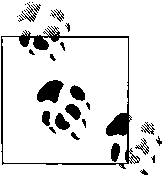
\includegraphics[width=2cm,clip]{paipai.png}
\end{wrapfigure}
\mbox{}\begin{flushleft}类似SunOS,SCO的Unix系统,提供一个free()的变种cfree(),它的行为跟具体的系统有关,有可能跟free()一 样,但也有可能接受三个参数,与calloc()相对.在Linux中,free()能处理我们现在涉及到的所有由动态存储机制分配到的内存。除非要考虑向下兼容的问题,不然我们不应该使用cfree()。所有Linux的版本中free()都是一样的。\end{flushleft}

要注意这个例子中如果不调用free()的结果。这个程序会永远也不将存储空间还给系统了,更为糟糕的是,唯一指向这块区域的指针s会消失,使得我们再也没有办法对这块内存进行操作。我们将这类编程错误叫做内存泄漏(memory leak)。内存泄漏以及其它一些动态内存产生的问题是很多程序中经常出现的,更不幸的是,这也是C语言编程中最可怕的小毛病。由于C语言将所有的内存管理交给程序员,所以程序员必须对于所有的内存分配格外注意。

另外一个最常见的错误是释放后再使用(use-after-free)。这个愚蠢的行为发生在一块内存被释放后,仍去访问它。一旦调用free()释放了某块内存,我们就再也不能对其进行操作了。程序员必须格外注意那些摇摆不定或指向不可使用内存块的指针。有两个常用的工具可以帮助你解决这些问题:Electric Fence和valgrind\footnote[1]{请见 http://perens.com/FreeSoftware/ElectricFence/ 以及 http://valgrind.org。}。

\subsection{对齐}

数据的对齐(alignment)是指数据地址和由硬件确定的内存块之间的关系。一个变量的地址是它大小的倍数时,就叫做自然对齐(naturally aligned)。例如,对于一个32bit长的变量,如果它的地址是4(字节)的倍数( 就是说,如果地址的低两位是0),那么这就是自然对齐了。所以,如果一个类型的大小是2n个字节,那么它的地址中,至少低n位是0。对齐的规则是根据硬件制定的。一些体系的计算机在数据对齐这方面有着很严格的要求。在有的系统中,载入一个没有对齐的数据将导致处理器的错误。在其它一些系统中,对不对齐的数据的访问是安全的,但却会引起性能的下降。在编写可移植的代码的时候,对齐的问题一定要注意,所有的类型都应该保持自然对齐。  

\subsubsection{预对齐内存的分配}

在大多数情况下,编译器和C库会自动处理对齐问题。POSIX规定通过malloc(),calloc()和realloc()返回的内存空间对于C中的标准类型都应该是对齐的。在Linux中,这些函数返回的地址在32位系统是以8字节为边界对齐,在64位系统是以16字节为边界对齐的。

有时候,对于更大的边界,例如页面,程序员需要动态的对齐。虽然动机是各不相同,但最基本的工作是将直接块I/O或是其它软硬件通信的缓冲区对齐。因此,POSIX 1003.1d提供一个叫做posix\_memalign()的函数: 

% \setmonofont{DejaVu Sans Mono}
\begin{lstlisting}
  /* one or the other -- either suffices */
  #define _XOPEN_SOURCE 600
  #define _GNU_SOURCE
  #include <stdlib.h>
  int posix_memalign (void **memptr,
                      size_t alignment,
                      size_t size);
\end{lstlisting}

调用posix\_memalign(),成功时会返回size字节的动态内存,并保证是按照alignment进行对齐的。参数alignment必须是2的幂,以及void指针大小的倍数。返回的内存块的地址保存在memptr里,函数返回0.

调用失败时,没有内存会被分配,memptr的值没有被定义,返回如下错误码之一: 

\begin{eqlist*}
\item[EINVAL] 参数不是2的幂,或者不是void指针的倍数。 
\item[ENOMEM] 没有足够的内存去满足函数的请求。 
\end{eqlist*}

要注意的是,对于这个函数,errno不会被设置,而是直接在返回值中给出。

由posix\_memalign()获得的内存通过free()释放。用法很简单: 

\begin{lstlisting}
  char *buf;
  int ret;
  /* allocate 1 KB along a 256-byte boundary */
  ret = posix_memalign (&buf, 256, 1024);
  if (ret) {
            fprintf(stderr, "posix_memalign: %s\n",
                     strerror (ret));
            return -1;
  }
  /* use 'buf'... */
  free (buf);
\end{lstlisting}

  更早的接口。在POSIX定义了posix\_memalign( )之前,BSD和SunOS分别提供了如下接口: 

% \setmonofont{DejaVu Sans Mono}
\begin{lstlisting}
  #include <malloc.h>
  void * valloc (size_t size);
  void * memalign (size_t boundary, size_t size);
\end{lstlisting}

函数valloc()的功能和malloc()一模一样,但返回的地址是页面对齐的。回顾一下第四章,页面的大小很容易通过getpagesize()得到。

相似地,函数memalign()是以boundary字节对齐的,而boundary必须是2的幂。在这个例子中,两个函数都返回一块足够大的内存去存放一个ship结构,并且地址都是在一个页面的边界上: 

\begin{lstlisting}
  struct ship *pirate, *hms;
  pirate = valloc (sizeof (struct ship));
  if (!pirate) {
               perror ("valloc");
               return -1;
  }
  hms = memalign (getpagesize ( ), sizeof (struct ship));
  if (!hms) {
            perror ("memalign");
            free (pirate);
            return -1;
  }
  /* use 'pirate' and 'hms'... */
  free (hms);
  free (pirate);
\end{lstlisting}

在Linux中,由这两个函数获得的内存都可以通过free()释放。但在别的Unix系统却未必是这样,一些系统并没有提供一个足够安全的机制来释放这些内存。出于移植性考虑,可能没有其他选择,但是注意不要使用free()去释放以上三个函数申请的内存。

只有为了移植到更老的系统上时,Linux的程序员才可以使用这两个函数。否则,应该优先选择posix\_memalign()。 这三个函数只有在malloc()的无法满足对齐需求时才使用。 

\subsubsection{其它对齐问题}

对齐问题不局限于标准类型与动态内存分配的自然对齐。比如说,复杂的数据类型的对齐问题将会比标准类型的更复杂。另外,在对不同类型的指针进行赋值以及强制类型转换的时候,对齐的问题也很重要。 

  非标准类型。非标准和复杂的数据类型的对齐比简单的自然对齐有着更多的要求。下面是四条有用的规则: 

\begin{itemize}
\item \begin{flushleft}一个结构的对齐要求和它的成员中最大的那个类型是一样的。例如,一个结构中最大的是以4字节对齐的32bit的整形,那么这个结构至少以4字节对齐。\end{flushleft}
\item \begin{flushleft}结构体也引入了对填充的需求,以此来保证每一个成员都符合各自的对齐要求。所以,如果一个char (可能以1字节对齐)后跟着一个int (可能以4字节对齐),编译器会自动地插入3个字节作为填充来保证int以4字节对齐。程序员们有时应该注意一下结构体中成员变量的顺序,来减少填充所导致的空间浪费。例如,可以将成员变量按照类型的大小进行排序。使用GCC编译时加入-Wpadded 选项可以帮助你应付这个问题。它会在填充时发出警告。\end{flushleft}
\item \begin{flushleft}一个联合的对齐和联合里最大的类型一致。 \end{flushleft}
\item \begin{flushleft}一个数组的对齐和数组里的元素类型一致。所以,除了对数组元素类型做对齐外,数组没有其他的对齐需求。这样可以使数组里面的所有成员都是自然对齐的。\end{flushleft}
\end{itemize}

  使用指针。因为编译器透明地处理了绝大多数的对齐问题,所以要找到潜在的错误的时候也比较困难。然而,这样的错误并不少见,特别是在处理指针和强转的时候。

假设一个指针从一个较少字节对齐的类型强转为一个较多字节对齐的类型,当通过这样的指针来访问时,会导致处理器不能对较多字节类型的数据正确对齐。例如,在如下的代码片段,c到badnews的强转使得程序将c当unsigned long来读: 

\begin{lstlisting}
  char greeting[] = "Ahoy Matey";
  char *c = greeting[1];
  unsigned long badnews = *(unsigned long *) c;
\end{lstlisting}

一个unsigned long 可能以4或8字节为边界对齐;而c当然只以1字节为边界对齐。因此当c被强转之后再进行读取将会导致对齐错误。这样的问题导致的后果,在不同的系统上各有不同,小者是性能损失,大者是整个程序崩溃。在可以发现而不能处理对齐错误的体系结构中,内核向出问题的进程发送SIGBUS信号来终止进程。我们会在第九章讨论信号。

像这样的例子在现实中出现的远远比你想的要多。当然现实中的例子肯定不会像这个一样明显,它们往往会更加隐蔽。 

\section{数据段的管理}

Unix系统在历史上提供过直接管理数据段的接口。然而,因为malloc()和其它的方法更强大也易于使用,大多数程序都不会直接地使用这些接口。我在这里说一下这些接口来满足一下大家的好奇心,同时也给那些想自己实现基于堆的动态分配机制的人一个参考: 

% \setmonofont{DejaVu Sans Mono}
\begin{lstlisting}
  #include <unistd.h>
  int brk (void *end);
  void * sbrk (intptr_t increment);
\end{lstlisting}

这些函数继承了一些老版本Unix系统中函数的名字,那时堆和栈还在同一个段中。堆中动态存储器的分配由数据段的底部向上生长;栈从数据段的顶部向着堆往下生长。堆和栈的分界线叫做中断(break)或中断点(break point)。在现代系统中,数据段存在于它自己的内存映射中,我们仍用中断点来标记映射的结束地址。

调用brk()会设置中断点(数据段的末端)的地址为end。在成功的时候,返回0。失败的时候,返回-1,并设置errno为ENOMEM。

调用sbrk()将数据段末端增加increment字节,increment可正可负。sbrk()返回修改后的断点。所以,increment为0时得到的是现在断点的地址: 

\begin{lstlisting}
  printf("The current break point is %p\n",sbrk(0));
\end{lstlisting}

尽管POSIX和C都没有定义这些函数。但几乎所有的Unix系统都至少支持其中之一。可移植的程序应该坚持使用基于标准的接口。 

\section{匿名存储器映射}

glibc的内存分配使用了数据段和内存映射。实现malloc( )最经典方法就是将数据段分为一系列的大小为2的幂的块,返回最小的符合要求的那个块来满足请求。释放则只是简单的将这块区域标记为未使用。如果相邻的分区都是空闲的,他们会被合成一个更大的分区。如果堆的最顶端是空的,系统可以用brk( )来降低断点,使堆收缩,将内存返回给系统。

这个算法叫做伙伴内存分配算法(buddy memory allocation scheme)。它的优点是高速和简单,缺点则是会产生两种类型的碎片。当使用的内存块大于请求的大小时则产生内部碎片(Internal fragmentation)。这导致了内存的低使用率。外部碎片是在空闲存储器合计起来足够满足一个请求,但是没有一个单独的空间块可以来处理这个请求时发生的。这同样会导致内存利用不足(因为可能会分配一个更大的块)或是分配的失败(如果已经没有可选的块存在了)。

另外,这个算法会使一个内存的分配“栓”住另外一个,导致glibc不能将释放的内存返回给系统。想象内存中已被分配的两个块,块A和块B。块A正好处在中断点的位置,块B刚好在A的下面,就算释放了B,在A被释放前,glibc也不能相应的调整中断点。在这种情况下,一个长期存在的内存分配就把另外的空闲空间“栓”住了。

不过不必为此担忧,因为glibc并不是一直在试图将空间返回给系统\footnote[1]{glibc也使用比这伙伴系统更加先进的存储分配算法,叫做arena 算法。}。通常来说,在每次释放后堆并不收缩。glibc会维护释放的内存以供之后的分配使用。只有当堆明显的大于已分配的内存时,glibc才会减小数据段的大小。从另一方面看,一个较大的分配会阻止这种收缩。 

因此,对于较大的分配,glibc并不使用堆而是创建一个匿名内存映射(anonymous memory mapping)来满足要求。匿名存储器映射和在第四章讨论的基于文件的映射很相似,只是它并不基于文件-所以称之为“匿名”。实际上,一个匿名内存映射只是一块已经用0初始化的大的内存块,以供用户使用。可以把它想成为单独为某次分配而使用的堆。因为这种映射的存储不是基于堆的,所以并不会在数据段内产生碎片。

使用匿名映射来分配内存有下列好处: 

\begin{itemize}
\item \begin{flushleft}无需关心碎片。当程序不再需要这块内存的时候,只要撤销映射,这块内存就直接归还给系统了。\end{flushleft}
\item \begin{flushleft}匿名存储映射的大小的是可调整的,可以设置权限,还能像普通的映射一样接受建议(看第四章)。\end{flushleft}
\item \begin{flushleft}每个分配存在于独立的内存映射。没有必要再去管理一个全局的堆了。\end{flushleft}
\end{itemize}

使用匿名映射与堆比起来也有两个缺点: 

\begin{itemize}
\item \begin{flushleft}每个存储器映射都是页面大小的整数倍。所以,如果大小不是页面整数倍的分配会浪费大量的空间。对于较小的分配来说,空间的浪费更加显著,因为相对于使用的空间,浪费的空间将更大。\end{flushleft}
\item \begin{flushleft}创建一个新的内存映射比从堆中返回内存的负载要大,因为使用堆几乎不涉及任何内核操作。越小的分配,这样的问题也越明显。\end{flushleft}
\end{itemize}

根据各自的优缺点来判断,glibc的malloc() 使用数据段来满足小的分配,而匿名内存映射则用来满足大的分配。两者的临界点是可调的(请参阅本章稍后的高级内存分配部分),并会随着glibc版本的不同而有所变化。目前,临界点一般是128KB:比128KB小的分配由堆实现,相应地,较大的由匿名存储器映射来实现。 

\subsection{创建匿名存储器映射}

或许你在某次分配想要使用一个内存映射而不是堆,又或者你正在写自己的内存分配系统,想要手工创建自己的匿名内存映射,不管怎么样,Linux都将让它变得非常简单。回忆一下第四章,用mmap()函数来创建内存映射,而用munmap()来销毁: 

% \setmonofont{DejaVu Sans Mono}
\begin{lstlisting}
  #include <sys/mman.h>
  void * mmap (void *start,
               size_t length,
               int prot,
               int flags,
               int fd,
               off_t offset);
  int munmap (void *start, size_t length);
\end{lstlisting}

因为不需要打开和管理文件,创建匿名存储器映射要比创建基于文件的存储器映射更简单。两者最关键的差别在于是否有匿名标记。让我们来看看这个例子: 

\begin{lstlisting}
  void *p;
  p = mmap (NULL, /* do not care where */
            512 * 1024, /* 512 KB */
            PROT_READ | PROT_WRITE, /* read/write */
            MAP_ANONYMOUS | MAP_PRIVATE, /* anonymous, private */
            -1, /* fd (ignored) */
            0); /* offset (ignored) */
  if (p == MAP_FAILED)
        perror ("mmap");
  else
        /* 'p' points at 512 KB of anonymous memory... */
\end{lstlisting}

对于大多数的匿名映射来说,mmap()的参数都跟这个例子一样。当然了,需要程序员确定映射大小的参数。其他参数大致如下: 

\begin{itemize}
\item \begin{flushleft}第一个参数是start,被设为NULL,意味着匿名映射可以让内核安排的在任意地址上。当然给定一个non-NULL值也是可以的,只要它是页对齐的,但这样会限制了可移植性。实际上很少有程序真正在意映射到哪个地址上去!\end{flushleft}
\item \begin{flushleft}prot参数经常都同时设置了PROT\_READ和PROT\_WRITE位,使得映射是可读可写的。一块不能读写的空存储器映射是没有用的。另外一方面,很少将可执行代码映射到匿名映射,因为那样做能产生潜在的安全漏洞。 \end{flushleft}
\item \begin{flushleft}flags参数设置MAP\_ANONYMOUS位,来使得映射是匿名的,设置MAP\_PRIVATE位,使得映射是私有的。 \end{flushleft}
\item \begin{flushleft}假如MAP\_ANONYMOUS被设置了,fd和offset参数将被忽略的。然而,在一些更早的系统里,需要让fd为-1,因此如果要考虑到程序的可移植性,那么这是一个好主意。 \end{flushleft}
\end{itemize}

匿名映射获得的内存块,看上去和由堆获得的一样。通过匿名映射进行分配的一个好处是所有的页都已经用0进行了初始化。由于内核使用写时复制(copy-on-write)将内存块映射到了一个全0的页面上,因而避免了额外的开销。同时也就没有必要对返回的内存块使用memset()。事实上这就是使用calloc()比先使用malloc()再使用memset()效果要好的原因之一:glibc知道匿名映射是本来就全0的了,使用该映射的calloc()则不需要再显式的置零了。系统调用munmap()释放一个匿名映射,归还已分配的内存给内核。 

\begin{lstlisting}
  int ret;
  /* all done with 'p', so give back the 512 KB mapping */
  ret = munmap (p, 512 * 1024);
  if (ret)
  perror ("munmap");
\end{lstlisting}

\begin{wrapfigure}{l}{2cm}
  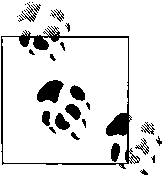
\includegraphics[width=1.5cm,clip]{paipai.png}
\end{wrapfigure}
\mbox{}\begin{flushleft}想复习一下mmap(),munmap(),和一般的映射,请参阅第四章。\end{flushleft}


\subsection{映射到/dev/zero}

其它Unix系统(例如BSD),并没有MAP\_ANONYMOUS标记。相反,它们使用特殊的设备文件/dev/zero实现了一个类似的解决方案。这个设备文件提供了和匿名内存相同的语义。一个包含全0的写时复制页面的映射;因此其行为和匿名存储器一致。 Linux一直支持/dev/zero设备,可以通过映射这个文件来获得全0的内存块。实际上,在引入MAP\_ANONYMOUS之前,Linux的程序员就使用该方法。为了对早期的Linux版本提供向下兼容或是为了移植到其它Unix系统上,程序员仍然可以将/dev/zero作为匿名映射替代方案。这与其他文件的映射没什么区别: 

\begin{lstlisting}
  void *p;
  int fd;
  /* open /dev/zero for reading and writing */
  fd = open ("/dev/zero", O_RDWR);
  if (fd < 0) {
              perror ("open");
              return -1;
  }
  /* map [0,page size) of /dev/zero */
  p = mmap (NULL, /* do not care where */
            getpagesize ( ), /* map one page */
            PROT_READ | PROT_WRITE, /* map read/write */
            MAP_PRIVATE, /* private mapping */
            fd, /* map /dev/zero */
            0); /* no offset */
  if (p == MAP_FAILED) {
                       perror ("mmap");
                       if (close (fd))
                       perror ("close");
                       return -1;
  }
  /* close /dev/zero, no longer needed */
  if (close (fd))
      perror ("close");
  /* 'p' points at one page of memory, use it... */ 
\end{lstlisting}

采用这种映射方式的存储器当然也是用munmap()来取消映射的。

然而这种方法因为要打开和关闭设备文件,所以会有额外的调用开销。因此匿名内存映射是一种较快的方法。 

\section{高级存储器分配}

本章所涉及的许多存储分配操作都是为内核的参数所控制和限制的,但程序员可以修改这些参数。为此,可以使用mallopt()函数: 

% \setmonofont{DejaVu Sans Mono}
\begin{lstlisting}
#include <malloc.h>
int mallopt (int param, int value);
\end{lstlisting}

调用mallopt()会将由param确定的存储管理相关的参数设为value。成功时,调用返回一个非0值;失败时,返回0。一般来说它都会正常返回,所以不要对能从返回值中获得什么抱太大的希望。

Linux目前支持六种param值,均被定义在了<malloc.h>中: 


\begin{eqlist*}
\item[M\_CHECK\_ACTION]环境变量MALLOC\_CHECK\_的值(将在下一节讨论)。 
\item[M\_MMAP\_MAX]系统用来满足动态存储器请求的最大存储器映射数。当达到这个限制时,分配就只能在数据段中进行,直到其中一个映射被释放。当该值为0时将禁止匿名映射用于动态存储的分配。 
\item[M\_MMAP\_THRESHOLD]决定该用匿名映射还是用数据段来满足存储器分配请求的阈值(以字节为单位)。要注意的是,有时候系统为了慎重起见,就算是比临界值小,也有可能用匿名映射来满足动态存储器的分配。值为0时会启用匿名映射来满足所有的分配,而不再使用数据段来满足请求。 
\item[M\_MXFAST]Fast bin的最大大小(以字节为单位)。Fast bins是堆中特殊的内存块,永远不和临近的内存块合并,也永远不归还给系统,以增加碎片为代价来满足高速的内存分配。值为0时,fasy bin将不被启用。 
\item[M\_TOP\_PAD]调整数据段的长度而使用的填充(padding)字节数。当glibc通过brk()来增加数据段的大小时,它可能申请更多的内存,希望减少很快再次调用brk()的可能性。相似地,但glibc收缩数据段的时候,它会保持一些多余的内存,而不是将所有的归还给系统。这多余的部分就称为填充。值为0时会取消使用填充。 
\end{eqlist*}

XPG中定义了mallopt(),并指定了另外三个参数:M\_GRAIN, M\_KEEP, 和M\_NLBLKS。Linux中定义了这些参数,但是实际上不起任何作用。表8-1定义了所有合法参数,他们的缺省值以及可接受的范围。 

\begin{center}
\begin{tabular}{ccccc}
  \toprule [1pt]
  \rowcolor[gray]{.9}
    参数 & 来源 & 缺省值 & 有效范围 & 特殊值来源 \\
  \midrule
    M\_CHECK\_ACTION & Linux特有 & 0 & 0-2 & 无 \\
	M\_GRAIN & XPG标准 & Linux不支持 & >=0 & 无 \\
	M\_KEEP & XPG标准 & Linux不支持 & >=0 & 无 \\
	M\_MMAP\_MAX & Linux特有 & 64*1024 & >=0 & 0禁用mmap() \\
	M\_MMAP\_THRESHOLD & Linux特有 & 128*1024 & >=0 & 0禁用堆 \\
	M\_MXFAST & XPG标准 & 64 & 0-80 & 0禁用fast bin \\
	M\_NLBLK & XPG标准 & Linux不支持 & >=0 & 无 \\
	M\_TOP\_PAD & Linux特有 & 0 & >=0 & 0禁用填充 \\
  \bottomrule[1pt]
\end{tabular}
\end{center}

程序必须要在调用malloc()或是其它内存分配函数前使用mallopt(),使用方法也非常简单: 

\begin{lstlisting}
  /* use mmap( ) for all allocations over 64 KB */
  ret = mallopt (M_MMAP_THRESHOLD, 64 * 1024);
  if (!ret)
      fprintf (stderr, "mallopt failed!\n");
\end{lstlisting}

\subsection{使用malloc\_usable\_size()和malloc\_trim()进行调优}

Linux提供了两个用来控制glibc内存分配系统的底层函数。第一个此类函数允许程序查询一块已分配内存中有多少可用字节: 

% \setmonofont{DejaVu Sans Mono}
\begin{lstlisting}
  #include <malloc.h>
  size_t malloc_usable_size (void *ptr);
\end{lstlisting}

调用malloc\_usable\_size()成功时,返回ptr指向的动态内存块的实际大小。因为glibc可能扩大动态内存来适应一个已存在的块或匿名映射,动态存储器分配中的可使用空间可能会比请求的大。当然,永远不可能比请求的小。下面是一个使用这个函数的例子: 

\begin{lstlisting}
  size_t len = 21;
  size_t size;
  char *buf;
  buf = malloc (len);
  if (!buf) {
            perror ("malloc");
            return -1;
  }
  size = malloc_usable_size (buf);
  /* we can actually use 'size' bytes of 'buf'... */
\end{lstlisting}

第二个函数允许程序强制glibc归还所有的可释放的动态内存给内核: 

 % \setmonofont{DejaVu Sans Mono}
\begin{lstlisting}
  #include <malloc.h>
  int malloc_trim (size_t padding);
\end{lstlisting}

调用malloc\_trim()成功时,数据段会尽可能地收缩,但是填充字节被保留下来。然后返回1。失败时,返回0。一般来说,每当空闲的内存到达M\_TRIM\_THRESHOLD 字节时,glibc会自动做这种收缩。使用M\_TOP\_PAD来用作填充。你不应该将这两个函数用于调试和教学以外的其它地方。它们是不可移植的,而且会将glibc内存分配系统的一些底层细节暴露给你的程序。 

\section{调试内存分配}

程序可以设置MALLOC\_CHECK\_环境变量来开启存储系统额外的调试功能。这个额外的调试检查是以降低内存分配的效率为代价的,然而这个开销在开发应用的调试阶段却是非常值得的。

因为仅仅一个环境变量就能控制调试,你不必重新编译你的程序。例如,你可以简单的执行如下指令: 

\begin{lstlisting}
$ MALLOC_CHECK_=1 ./rudder
\end{lstlisting}

如果设置为0,存储系统会忽略所有错误。如果它被设为1了,信息会被输出到标准错误输出stderr。如果设置为2,进程会立即通过abort( )终止。因为 MALLOC\_CHECK\_ 会改变正在运行的程序的行为,所以setuid程序忽略这个变量。 

\subsection{获得统计数据}

Linux提供了mallinfo()函数来获得关于动态存储分配系统的统计数据: 

% \setmonofont{DejaVu Sans Mono}
\begin{lstlisting}
  #include <malloc.h>
  struct mallinfo mallinfo (void);
\end{lstlisting}

mallinfo()的调用将统计数据保存到mallinfo结构中。这个结构是通过值而不是指针返回的。它的字段结构也在<malloc.h>定义了。

\begin{lstlisting}
  /* all sizes in bytes */
  struct mallinfo {
     int arena; /* malloc使用的数据段的大小 */
     int ordblks; /* 空闲块的个数 */
     int smblks; /* fast bin 的个数 */
     int hblks; /* 匿名映射的个数 */
     int hblkhd; /* 匿名映射的大小 */
     int usmblks; /* 最大已分配值 */
     int fsmblks; /* 可用的fast bin的大小 */
     int uordblks; /* 所有的被分配的空间 */
     int fordblks; /* 可用的块大小 */
     int keepcost; /* 可消去的多余空间的大小 */};
\end{lstlisting}


用法很简单: 

\begin{lstlisting}
  struct mallinfo m;
  m = mallinfo();
  printf ("free chunks: %d\n", m.ordblks);
\end{lstlisting}

Linux 也提供了malloc\_stats()函数,将跟内存相关的统计数据打印到标准错误输出(stderr): 

% \setmonofont{DejaVu Sans Mono}
\begin{lstlisting}
  #include <malloc.h>
  void malloc_stats (void);
\end{lstlisting}

在内存操作频繁的程序中调用往往会产生一些较大的数字: 

\begin{verbatim}
  Arena 0:
  system bytes = 865939456
  in use bytes = 851988200
  Total (incl. mmap):
  system bytes = 3216519168
  in use bytes = 3202567912
  max mmap regions = 65536
  max mmap bytes = 2350579712
\end{verbatim}

\section{基于栈的分配}

到目前为止,我们学过的所有的动态内存分配机制都是使用堆和存储器映射来实现的。我们很自然的想到使用它们因为堆和匿名映射本身就是动态的。另外一个在程序地址空间中常用的结构,栈,是用来存放程序的自动变量(automatic variables)的。

然而,认为程序员不能使用栈来进行动态内存分配是毫无理由的。只要一个分配不使栈溢出,这样的做法是简单而完美的。如果要在一个栈中实现动态内存分配,使用系统调用alloca():

% \setmonofont{DejaVu Sans Mono}
\begin{lstlisting}
  #include <alloca.h>
  void * alloca (size_t size);
\end{lstlisting}

调用alloca(),成功时会返回一个指向size字节大小的内存指针。这块内存是在栈中的,当调用它的函数(例如main函数)返回时,这块内存将被自动释放。某些该函数的实现会在失败时返回NULL,但是大部分时候alloca()都不可能失败,或是不可能报告失败。失败就表明出现的栈溢出。

用法与malloc()一样,但你不必(实际上,是不能)释放分配到的内存。以下示例函数,在系统配置目录(可能是/etc) 里面打开一个给定的文件,目录在编译时就被确定了。这个函数必须申请一个新的缓冲区,复制系统配置路径到这个缓冲区里面,然后将提供的文件名拼接到缓冲区的后面: 

\begin{lstlisting}
  int open_sysconf (const char *file, int flags, int mode)
  {
    const char *etc = SYSCONF_DIR; /* "/etc/" */
    char *name;
    name = alloca (strlen (etc) + strlen (file) + 1);
    strcpy (name, etc);
    strcat (name, file);
    return open (name, flags, mode);
  }
\end{lstlisting}

在open\_sysconf函数返回时,从alloca()分配到的内存随着栈的收缩而被自动释放。这意味着当调用alloca()的函数返回后,你不能再使用由alloca()得到的那块内存!然而,你并不需要做任何释放工作,所以最终代码会简洁一些。下面是一个通过malloc()实现的相同的函数: 

\begin{lstlisting}
  int open_sysconf (const char *file, int flags, int mode)
  {
      const char *etc = SYSCONF_DIR; /* "/etc/" */
      char *name;
      int fd;
      name = malloc (strlen (etc) + strlen (file) + 1);
      if (!name) {
                 perror ("malloc");
                 return -1;
      }
      strcpy (name, etc);
      strcat (name, file);
      fd = open (name, flags, mode);
      free (name);
      return fd;
  }
\end{lstlisting}

要注意的是你不能使用由alloca()得到的内存来作为一个函数调用的参数,因为分配到的内存块会被当做参数保存在函数的栈中。例如,下面这样做是不行的: 

\begin{lstlisting}
  /* DO NOT DO THIS! */
  ret = foo (x, alloca (10));
\end{lstlisting}

alloca() 接口有着曲折的历史。在许多系统,它表现得非常差,或者出现没被定义的行为。在栈大小较小而且是确定的系统中,使用alloca()很容易出现栈溢出,导致程序崩溃。在另外一些系统中,alloca()甚至就不存在。由于经常出错和不稳定,人们对alloca()总是没有一个好的印象。

所以,如果要让代码具有可移植性,你要避免使用alloca()。然而在Linux系统上,alloca()却是一个非常好用但没有被人们认识到的工具。它表现的异常出色(在各种架构下,通过alloca()进行内存分配就和增加栈指针一样简单),比malloc()的性能要好很多。对于Linux下较小的内存分配,alloca()能收获让人激动的性能。 

\subsection{栈中的复制串}

alloca()常见的用法是用来临时复制一个字符串。例如: 

\begin{lstlisting}
  /* we want to duplicate 'song' */
  char *dup;
  dup = alloca (strlen (song) + 1);
  strcpy (dup, song);
  /* manipulate 'dup'... */
  return; /* 'dup' is automatically freed */
\end{lstlisting}

因为这种需求非常多以及alloca()实现的高效,Linux系统专门提供了strdup()来将一个给定的字符串复制到栈中: 

% \setmonofont{DejaVu Sans Mono}
\begin{lstlisting}
  #define _GNU_SOURCE
  #include <string.h>
  char * strdupa (const char *s);
  char * strndupa (const char *s, size_t n);
\end{lstlisting}

调用strdupa( )会返回一个s的拷贝。strndupa()将拷贝s中的n个字符。如果s长度大于n,就复制s前n个字节,然后后面自动加上一个空字节。这些函数具有alloca()的优点。当调用函数返回时,复制的串会自动释放。 POSIX并没有定义alloca( ), strdupa( ),或者strndupa( )函数,它们在别的操作系统的表现也差强人意。如果考虑到可移植性,不鼓励使用这些函数。然而在Linux上,alloca()以及由它衍生的一些函数却表现的非常好,可以通过简单的移动栈指针来代替其它一些复杂动态分配内存方法,从而带来性能上的提升。

\subsection{变长数组}

C99 引进了变长数组(VLAs),变长数组的长度是在运行时决定的,而不是在编译的时候。。在这之前,GNUC已经支持变长数组了,但是现在C99将其标准化,因此对于变长数组的使用得到了很大的鼓励。VLAs用与alloca()相似的方法避免了动态存储分配所产生的负载。它的使用方法就跟你想象的一样: 

\begin{lstlisting}
  for (i = 0; i < n; ++i) {
      char foo[i + 1];
      /* use 'foo'... */
  }
\end{lstlisting}

在这个代码片段中,foo是一个有i+1个char的数组。在每次循中,foo都被动态的创建,并在这轮循环结束时自动释放。如果我们使用alloca()来代替VLA,那么内存空间将直到函数返回时才会被释放。使用一个VLA确保了内存每次循环都被释放。所以,使用VLA最多使用n个字节,而alloca()会使用掉n*(n+1)/2个字节。使用一个变长数组,我们能够像这样重写我们的open\_sysconf()函数: 

\begin{lstlisting}
  int open_sysconf (const char *file, int flags, int mode)
  {
      const char *etc; = SYSCONF_DIR; /* "/etc/" */
      char name[strlen (etc) + strlen (file) + 1];
      strcpy (name, etc);
      strcat (name, file);
      return open (name, flags, mode);
  }
\end{lstlisting}

alloca()和变长数组的主要区别在于通过前者获得的内存在函数执行过程中始终存在,而通过后者获得的内存在出了作用域后便释放了。这样的方式有好有坏。在for循环中,我们希望每次循环都能释放空间以在没有任何副作用的情况下减小内存的开销(我们不会希望有多余的内存始终被占用着)。然而,如果出于某种原因我们希望这块空间能保留到下一轮的循环中,那么使用alloca()显然是更加合理的。

\begin{wrapfigure}{l}{2.5cm}
  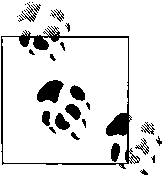
\includegraphics[width=2cm,clip]{paipai.png}
\end{wrapfigure}
\mbox{}\begin{flushleft}在单个函数中混淆了alloca()和变长数组会给程序引入怪异的行为。因此为了安全起见在一个固定的函数中只应使用其中之一。 \end{flushleft}

\section{选择一个合适的内存分配机制}

本章中讨论了很多种内存分配的方式,这可能使得程序员们不清楚在一个具体的问题中到底该使用哪一种。在大部分的情况下malloc()总是最好的选择。然而在某些情况下,采用其它方法会更好一些。表8-2总结了一些选择内存分配机理的原则: 

\begin{center}
\begin{tabular}{p{3cm}p{5cm}p{5cm}}
  \toprule [1pt]
  \rowcolor[gray]{.9}
    分配方式 & 优点 & 缺点 \\
  \midrule
    malloc() & 简单,方便,最常用 & 返回的内存为用零初始化   \\
    calloc() & 使数组分配变得容易,
	
	用0初始化了内存 & 在分配非数组空间时显得较复杂   \\
    realloc() & 调整已分配的空间大小 & 只能用来调整已分配空间的大小  \\
    brk()和sbrk() & 允许对堆进行深入控制 & 对大多数使用者来说过于底层  \\
    匿名内存映射 & 使用简单,可共享,允许开发者调整保护等级并提供建议,适合大空间的分配 & 不适合小分配。最优时malloc()会自动使用匿名内存映射 \\
    posix\_memalign() & 分配的内存按照任何合理的大小进行对齐 & 相对较新,因此可移植性是一个问题;对于对齐的要求不是很迫切的时候,则没有必要使用\\
    memalign()和valloc() & 相比posix\_memalign()在其它的Unix系统上更常见 & 不是POSIX标准,对对齐的控制能力不如posix\_memalign() \\
    alloca() & 最快的分配方式,不需要知道确切的大小,对于小的分配非常适合 & 不能返回错误信息,不适合大分配,在一些Unix系统上表现不好 \\
    变长数组 & 与alloca()类似,但在退出此层循环是释放空间,而不是函数返回时 & 只能用来分配数组,在一些情况下alloca()的释放方式更加适用,在其它Unix系统中没有alloca()常见 \\
  \bottomrule[1pt]
\end{tabular}
\end{center}

最后我们不能忘记以上方式之外的两个选择: 静态分配和自动分配。在栈中分配临时变量以及在堆中分配全局变量总是最简单的,而且不需要程序员们控制指针以及释放内存。 

\section{存储器操作}

C语言提供了很多函数进行内存操作。这些函数的功能和字符串操作函数(如strcmp()以及strcpy())类似,但是他们处理的对象是用户提供的内存区域而不是以NULL结尾的字符串。要注意这些函数都不会返回错误信息。因此防范错误是程序员的责任,如果传递错误的内存区域作参数的话,你将毫无疑问的得到段错误。 

\subsection{字节设置}

在一系列的内存操作函数当中,最常用的是memset(): 

% \setmonofont{DejaVu Sans Mono}
\begin{lstlisting}
  #include <string.h>
  void * memset (void *s, int c, size_t n);
\end{lstlisting}

调用memset()将把从s指向区域开始的n个字节设置为c,并返回s。它经常被用来将一块内存清零: 

\begin{lstlisting}
  /* zero out [s,s+256) */
  memset (s, '\0', 256);
\end{lstlisting}

bzero()是早期由BSD引入的相同功能的函数,现在已被淘汰。新的代码应该使用memset(),但Linux出于向下兼容和对其它系统的可移植性的考虑,也提供了bzero():

% \setmonofont{DejaVu Sans Mono}
\begin{lstlisting}
  #include <strings.h>
  void bzero (void *s, size_t n);
\end{lstlisting}

下面的调用功能和先前memset()的例子一样: 

\begin{lstlisting}
  bzero (s, 256);
\end{lstlisting}

注意bzero()(其它b开头的函数也是如此)需要头文件<strings.h>而不是<string.h>。

\begin{wrapfigure}{l}{2.5cm}
  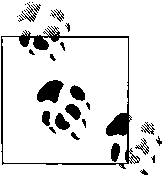
\includegraphics[width=2cm,clip]{paipai.png}
\end{wrapfigure}
\mbox{}\begin{flushleft}如果你可以使用calloc()分配内存那就坚决不要使用memset()了。不要先用malloc()分配了内存,再马上使用 memset()来进行清零。虽然结果可能是一样的,但是将这两次调用合并成直接返回已经清零了的空间calloc()会更好。好处在于你不仅少了一次函数调用,而且calloc()是直接从内存中获取已经清零了的内存,这显然比手工的将每个字节清零要高效。\end{flushleft}

\subsection{字节比较}

和strcmp()相似,memcmp()比较两块内存是否相等: 

% \setmonofont{DejaVu Sans Mono}
\begin{lstlisting}
  #include <string.h>
  int memcmp (const void *s1, const void *s2, size_t n);
\end{lstlisting}

调用memcmp()比较s1和s2的头n个字节,如果两块内存相同就返回0,如果s1小于s2就返回一个小于0的数,反之则返回大于0的数。

BSD同样提供了自己具有类似功能的接口:

% \setmonofont{DejaVu Sans Mono}
\begin{lstlisting}
  #include <strings.h>
  int bcmp (const void *s1, const void *s2, size_t n);
\end{lstlisting}

调用bcmp()会比较s1和s2的前n字节,如果两块内存就一样返回0,否则返回非0值。因为结构填充的存在(参照本章之前的“其它对齐问题”),通过memcmp()或者bcmp()来比较两个结构是否相等是不可靠的。同一个结构的两个实例也可能因为有未初始化的填充内容而被判为不相等。因此,下面的代码是不安全的: 

\begin{lstlisting}
  /* are two dinghies identical? (BROKEN) */
  int compare_dinghies (struct dinghy *a, struct dinghy *b)
  {
      return memcmp (a, b, sizeof (struct dinghy));
  }
\end{lstlisting}

程序员们如果想要比较结构体,只能一个一个比较结构体中的每一个元素。下面这个方法实现了一些优化,但它的工作量当然会比不安全的memcmp()要大: 

\begin{lstlisting}
  /* are two dinghies identical? */
  int compare_dinghies (struct dinghy *a, struct dinghy *b)
  {
      int ret;
      if (a->nr_oars < b->nr_oars)
          return -1;
      if (a->nr_oars > b->nr_oars)
          return 1;
      ret = strcmp (a->boat_name, b->boat_name);
      if (ret)
          return ret;
      /* and so on, for each member... */
  }
\end{lstlisting}

\subsection{字节移动}

memmove()复制src的前n字节到dst,返回dst: 

% \setmonofont{DejaVu Sans Mono}
\begin{lstlisting}
  #include <string.h>
  void * memmove (void *dst, const void *src, size_t n);
\end{lstlisting}

同样,BSD提供了一个被批评的接口来实现相同的功能: 

% \setmonofont{DejaVu Sans Mono}
\begin{lstlisting}
  #include <strings.h>
  void bcopy (const void *src, void *dst, size_t n);
\end{lstlisting}

需要指出的是尽管两个函数的参数相同,但是它们的位置是不一样的,在bcopy()中前两个参数的位置是反的。

bcopy()和 memmove()可以安全地处理内存区域重叠问题(就是说,dst的一部分在src 里面)。例如,它们允许内存块在一个给定的区域内向上或下移动。虽然这种情况很少见,但是程序员应该知道有这么一回事。所以C标准定义了一个不支持内存区域覆盖的memmove()变种。这个变种可能会快一点: 

% \setmonofont{DejaVu Sans Mono}
\begin{lstlisting}
  #include <string.h>
  void * memcpy (void *dst, const void *src, size_t n);
\end{lstlisting}

除了dst和src间不能重叠,这个函数基本和memmove()一样。如重叠了,函数的结果是未被定义的。另外一个安全的复制函数是memccpy(): 

% \setmonofont{DejaVu Sans Mono}
\begin{lstlisting}
  #include <string.h>
  void * memccpy (void *dst, const void *src, int c, size_t n);
\end{lstlisting}

memccpy()和memcpy()类似,但当它发现字节c在src指向的前n个字节中时会停止拷贝。它返回指向dst中c后一个字节的指针,或者当没有找到c时返回NULL。

最后我们可以使用mempcpy()来跨过拷贝的内存: 

% \setmonofont{DejaVu Sans Mono}
\begin{lstlisting}
  #define _GNU_SOURCE
  #include <string.h>
  void * mempcpy (void *dst, const void *src, size_t n);
\end{lstlisting}

函数mempcpy()和memcpy()几乎一样,区别在于memccpy()返回的是指向被复制的内存的最后一个字节的下一个字节的指针。当在内存中有连续的一系列数据需要拷贝时它是很有用的。但是它并没有太大的性能提升,因为返回的指针只是dst+n而已。这个函数是GNU中特有的。 

\subsection{字节搜索}

函数memchr()和memrchr()可以在内存块中搜索一个给定的字节: 

% \setmonofont{DejaVu Sans Mono}
\begin{lstlisting}
  #include <string.h>
  void * memchr (const void *s, int c, size_t n);
\end{lstlisting}

函数memchr()从s指向的区域开的n个字节中寻找c,c将被转换为unsigned char: 

% \setmonofont{DejaVu Sans Mono}
\begin{lstlisting}
  #define _GNU_SOURCE
  #include <string.h>
  void * memrchr (const void *s, int c, size_t n);
\end{lstlisting}

函数返回指向第一个匹配c的字节的指针,如果没找到c则返回NULL。

memrchr()与memchr()类似,不过它是从s指向的内存开始反向搜索n个字节。和memchr()不同,memrchr()是GNU的扩展函数,而不是C语言的一部分。 对于更加复杂的搜索,有个名字很烂的memmem()函数,它可以在一块内存中搜索任意的字节数组: 

% \setmonofont{DejaVu Sans Mono}
\begin{lstlisting}
  #define _GNU_SOURCE
  #include <string.h>
  void * memmem (const void *haystack,
                 size_t haystacklen,
                 const void *needle,
                 size_t needlelen);
\end{lstlisting}

memmem()函数在指向长为haystacklen的内存块haystack中查找,并返回第一块和长为needlelen的needle匹配的子块的指针。如果函数在haystack中不能找到needle,它会返回NULL。这个函数同样是GNU的扩展函数。 

\subsection{字节加密}

Linux的C库提供了进行简单数据加密的接口:

% \setmonofont{DejaVu Sans Mono}
\begin{lstlisting}
  #define _GNU_SOURCE
  #include <string.h>
  void * memfrob (void *s, size_t n);
\end{lstlisting}

memfrob()函数将s指向的位置开始的n个字节,每个都与42进行异或操作来对数据进行加密。函数返回s。

再次对相同的区域调用memfrob()可以将其转换回来。因此下面这行程序对于secret没有进行什么实质性的操作: 

\begin{lstlisting}
  memfrob (memfrob (secret, len), len);
\end{lstlisting}

这个函数用于数据加密时绝对不合适的(甚至是更差的);它的使用仅限于对于字符串的简单处理。它是GNU标准函数。 

\section{内存锁定}

Linux 实现了请求页面调度,页面调度是说在需要时将页面从硬盘交换进来,当不再需要时再交换出去。这使得系统中进程的虚拟地址空间与实际的物理内存大小没有直接的关系,同时硬盘上的交换空间提供一个拥有近乎无限物理内存的假象,

交换对进程来说是透明的,应用程序一般都不需要关心(甚至不需要知道)内核页面调度的行为。然而,在下面两种情况下,应用程序可能希望影响系统的页面调度: 

\begin{eqlist*}
\item[确定性(Determinism)] 时间约束严格的应用程序需要自己来决定页的调度行为。如果一些内存操作引起了页错误-这会导致昂贵的磁盘操作-应用程序则可能会超出要求的运行时间。如果能确保需要的页面总在内存中且从不被交换进磁盘,应用程序就能保证内存操作不会导致页错误,提供一致的,可确定的程序行为,从而提供了效能。 
\item[安全性(Security)]如果内存中含有私人信息,这些信息可能最终被页面调度以不加密的方式储存到硬盘上。例如,如果一个用户的私钥正常情况下是以加密的方式保存在磁盘上的,一个在内存中未加密的密钥备份最后可能保存在了交换文件中。在一个高度注重安全性的环境中,这样做可能是不可接受。这样的应用程序可以请求将密钥一直保留在物理内存上。
\end{eqlist*}

当然,改变内核的行为可能会对系统整体的表现产生负面的影响。应用的确定性和安全性可能会提高,但是当它的页被锁在了内存中,那另一个应用的页就只能被换出内存。如果我们相信内核的设计,那么它将总是把最优的页换出,也就是那些在未来最有可能被访问的页。因此如果你改变的它的行为,那么它就只能将一个次优的页换出了。

\subsection{锁定部分地址空间}

POSIX1003.1b-1993定义两个接口将一个或更多的页面“锁定”在物理内存,来保证它们不会被交换到磁盘。第一个函数锁定给定的一个地址区间: 

% \setmonofont{DejaVu Sans Mono}
\begin{lstlisting}
  #include <sys/mman.h>
  int mlock (const void *addr, size_t len);
\end{lstlisting}

调用mlock()将锁定addr开始长度为len个字节的虚拟内存。成功的话,函数返回0;失败时,函数返回-1,并适当设置errno。

成功调用会将所有包含[addr,addr+len)的物理内存页锁定。例如,一个调用只是指定了一个字节,包含这个字节的所有物理页都将被锁定。POSIX标准要求addr应该与页边界对齐。Linux并没有强制要求,如果真要这样做的时候,会悄悄的将addr向下调整到最近的页面。对于要求可移植到其它系统的程序需要保证addr是页对齐的。

合法的errno包括: 

\begin{eqlist*}
\item[EINVAL] 参数len是负数。 
\item[ENOMEM] 函数尝试锁定多于RLIMIT\_MEMLOCK限制的页(详见之后“锁定限制”部分)。
\item[EPERM] RLIMIT\_MEMLOCK是0,但进程并没有CAP\_IPC\_LOCK权限。(同样请见“锁定限制”部分)。
\end{eqlist*}

\begin{wrapfigure}{l}{2.5cm}
  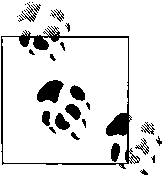
\includegraphics[width=2cm,clip]{paipai.png}
\end{wrapfigure}
\mbox{}\begin{flushleft}一个由fork()产生的子进程并不从父进程处继承锁定的内存。然而,由于Linux对地址空间写时复制机制,子进程的页面被锁定在内存中直到子进程对它们执行写操作。 \end{flushleft}

下面这个例子,假设一个程序在内存中有一个加密的字符串。一个进程可以通过下面代码来锁定拥有这个字符串的页: 

\begin{lstlisting}
  int ret;
  /* lock 'secret' in memory */
  ret = mlock (secret, strlen (secret));
  if (ret)
     perror ("mlock");
\end{lstlisting}

\subsection{锁定全部地址空间}

如果一个进程想在物理内存中锁定它的全部地址空间,使用mlock()就不再合适了。POSIX定义了mlockall()函数来满足这个实时应用中常见的需求: 

% \setmonofont{DejaVu Sans Mono}
\begin{lstlisting}
  #include <sys/mman.h>
  int mlockall (int flags);
\end{lstlisting}

mlockall()函数锁定一个进程在现有地址空间在物理内存中的所有页面。flags参数,是下面两个值的按位或操作,用以控制函数行为: 

\begin{eqlist*}
\item[MCL\_CURRENT] 如果设置了该值,mlockall()会将所有已被映射的页面(包括栈,数据段,映射文件)锁定进程地址空间中。 
\item[MCL\_FUTURE] 如果设置了该值,mlockall()会将所有未来映射的页面也锁定到进程地址空间中。
\end{eqlist*}

大部分应用程序都会同时设定这两个值。成功时,函数返回0;失败时,返回-1,并设置errno为下列错误码之一: 

\begin{eqlist*}
\item[EINVAL] 参数len是负数。
\item[ENOMEM] 函数要锁定的页面数比RLIMIT\_MEMLOCK限制的要多(详见之后“锁定限制”部分)。
\item[EPERM] RLIMIT\_MEMLOCK是0,但进程并没有CAP\_IPC\_LOCK权限。(同样请见“锁定限制”部分)。
\end{eqlist*}

\subsection{内存解锁}

POSIX标准提供了两个接口用来将页从内存中解锁,允许内核根据需要将页换出至硬盘中: 

% \setmonofont{DejaVu Sans Mono}
\begin{lstlisting}
  #include <sys/mman.h>
  int munlock (const void *addr, size_t len);
  int munlockall (void);
\end{lstlisting}

系统调用munlock()解除addr开始长为len的内存所在的页面地锁定。它消除mlock()的效果。而munlockall()则消除mlockall()的效果。两个函数在成功时都返回0,失败时返回-1,像如下设置errno: 

\begin{eqlist*}
\item[EINVAL] 参数 len 是负数(仅对munlock())。
\item[ENOMEM] 被指定的页面中有些是不合法的。
\item[EPERM] RLIMIT\_MEMLOCK是0,但进程并没有CAP\_IPC\_LOCK权限。(同样请见“锁定限制”部分)。
\end{eqlist*}

内存锁定并不会重叠。所以,不管被mlock()或mlockall()锁定了多少次,仅一个mlock()或者munlock(),即会解除一个页面的锁定。 

\subsection{锁定的限制}

因为内存的锁定能影响一个系统的整体性能-实际上,如果太多的页面被锁定,内存分配会失败------Linux对于一个进程能锁定的页面数进行了限制。

拥有CAP\_IPC\_LOCK权限的进程能锁定任意多的页面。没有这个权限的进程只能锁定RLIMIT\_MEMLOCK个字节。默认情况下,该限制是32KB(足够将一两个秘密信息锁定在内存中)对系统性能也没有什么负面影响。(第6章讨论资源限制和怎样找到和设置这些值) 

\subsection{这个页面在物理内存中吗?}

出于调试的需要,Linux提供了mincore()函数,可以用来确定一个给定范围内的内存是在物理内存中还是被交换到了硬盘中: 

% \setmonofont{DejaVu Sans Mono}
\begin{lstlisting}
  #include <unistd.h>
  #include <sys/mman.h>
  int mincore (void *start,
               size_t length,
               unsigned char *vec);
\end{lstlisting}

调用mincore()提供了一个向量,表明调用时刻映射中哪个页面是在物理内存中。函数通过vec来返回向量,这个向量描述start(必需页面对齐)开始长为length(不需要对其)字节的内存中的页面的情况。vec的每个字节对应指定区域内的一个页面,第一个字节对应着第一个页面,然后依次对应。因此,vec必须足够大来装入(length-1+page size)/page size字节。如果那页面在物理内存中,对应字节的最低位是1,否则是0。其它的位目前还没有定义,留待日后使用。

成功时,函数返回0。失败时,返回-1,并设置errno为如下值之一: 

\begin{eqlist*}
\item[EAGAIN] 内核目前没有足够的可用资源来满足请求。
\item[EFAULT] 参数vec指向一个非法地址。
\item[EINVAL] 参数start不是页对齐。
\item[ENOMEM] [address,address+1) 中的内存不在某个基于文件的映射中。
\end{eqlist*}

目前来说, 这个系统调用只能用在以MAP\_SHARED创建的基于文件的映射上。这在很大程度上限制了这个函数的使用。 

\section{投机性存储分配策略}

Linux 使用投机分配策略。当一个进程向内核请求额外的内存-如扩大它的数据段,或者创建一个新的存储器映射-内核作出了分配承诺但实际上并没有分给进程任何的物理存储。仅当进程对新“分配到”的内存区域作写操作的时候,内核才履行承诺,分配一块物理内存。内核逐页完成上述工作,并在需要时进行请求页面调度和写时复制。

这样处理有如下几个优点。首先,延缓内存分配允许内核将大部分工作推迟到最后一刻(当确实需要进行分配时)。第二,由于请求是根据需求逐页的分配,只有真正需要物理内存的时候才会消耗物理存储。最后,分配到的内存可能比实际的物理内存甚至比可用的交换空间多得多。最后这个特征叫做超量使用(overcommitment)。 

\subsection{超量使用和内存耗尽}

和在应用请求页面就分配物理存储相比,在使用时刻才分配物理存储的过量使用机制允许系统运行更多,更大的应用程序。如果没有超量使用,用写时复制映射2GB文件需要内核划出2GB的物理存储。采用超量使用,映射2GB文件需要的存储量仅仅是进程映射区域中真正进行写操作的所有页面的大小。同样,没有超量使用,就算大多数页面都不需要进行写时拷贝,每个fork()操作都需要申请空闲内存来复制整个地址空间。

但是,如果系统中的进程为满足超量使用而申请的内存大于物理内存和交换空间之和,这时会怎样呢?在这种情况下,一个或者更多的分配一定会失败。因为内核已经承诺给进程分配内存了(系统调用成功返回),而这个进程尝试使用已分配的内存,内核只能杀死另一个进程并释放它的内存,以此来满足下一次的分配需求。

当超量使用导致内存不足以满足一个请求时,我们就说发生了内存耗尽(OOM)(out of memory)。为了处理OOM,内核使用OOM 终结者(killer)来挑选一个进程,并终止它。基于这个目的,内核会尝试选出一个最不重要且又占用很多内存的进程。

OOM 其实很少出现-所以采用效果非凡的超量使用非常有实际意义的。然而,可以肯定的是,没人希望发生OOM,而且进程突然被OOM 终结者(killer)终结了也往往是无法接受。

对于不想这种情况出现的系统,内核允许通过文件/proc/sys/vm/overcommit\_memory关闭超量使用,和此功能相似的还有sysctl的vm.overcommit\_memory参数。

参数的默认值是0,告诉内核执行适度的超量使用策略,在合理范围内实施超量使用,超出限定值时则不可使用。值为1时,确认所有的分配请求,将一切顾虑抛诸脑后。一些对存储要求较高的应用程序,(例如在科学计算领域)倾向于请求比他们实际需要更多的内存,这时这个参数值就很有帮助。

当值为2时,关闭所有的过量使用,启用严格审计(strict accounting)策略。这个模式中,承诺的内存大小被严格限制在交换空间大小加上可调比例的物理内存大小。这个比例可以在文件/proc/sys/vm/overcommit\_ratio里面设置,作用和vm.overcommit\_ratio的sysctl参数相似。 默认是50,限制承诺的内存总量是交换空间加上物理内存的一半。因为物理内存还必须包含着内核,页表,系统保留页,锁定页等等东西。仅它的一部分能被交换和满足承诺请求。

使用严格审计策略时要非常小心!许多系统设计者,被OOM终结者(killer)的思想,搞得崩溃了,认为严格审计才是解决之道。然而,应用程序常常进行一些不必要的、且只有使用超量使用才能满足的分配请求,而允许这种行为也是设计虚拟内存的主要动机之一。 

\ifx\atempxetex\usewhat
\XeTeXinputencoding "utf-8"
\fi
\defaultfont

\chapter{信号}

信号是提供处理异步事件机制的软件中断。这些事件可以来自系统外部——例如用户产生中断符(通常是Ctrl-C)——或者来自程序或内核内部的活动,例如进程执行除以零的代码。作为一种进程间通信(IPC)的基本形式,进程也可以给另一个进程发送信号。

关键问题不仅仅是事件的发生是异步的(例如用户可以在程序执行的任何时候按下Ctrl-C)而且程序对信号的处理也是异步的。信号处理函数在内核注册,收到信号时,内核从程序的其它部分异步地调用信号处理函数。

信号很早就是Unix的一部分。随着时间的推移,信号有了很大的改进。比如在可靠性方面,之前的信号可能会出现丢失的情况;在功能方面,现在信号可以携带用户定义的附加信息。最初,不同的Unix系统对信号做了不同的改变。值得庆幸的是,POSIX标准的到来挽救并且标准化了信号处理。这个标准正是Linux提供的,并且也是我们这里将要讨论的。

在本章中,我们从信号概述开始,并且讨论它们的使用和误用。接下来我们会讨论各种Linux管理和操作信号的接口。

大多数杰出的应用程序都与信号有关。即使你故意设计不依赖信号来进行通讯的应用程序(这通常是一个好主意),在某些特殊的情况下你仍然会被迫使用信号,例如处理程序终止。

\section{信号概念}

信号有一个非常明确的生命周期。首先,产生信号(我们有时也说信号被发出或生成)。然后内核存储信号直到可以发送它。最后,一旦有空闲,内核会适当的处理信号。内核根据进程的请求可以执行以下三个过程之一: 

\begin{eqlist*}
\item[忽略信号] 不采取任何操作。但是有两种信号不能被忽略:SIGKILL和SIGSTOP。这样做的原因是系统管理员需要能够杀死或停止进程,如果进程能够选择忽略SIGKILL(使进程不能被杀死)或SIGSTOP(使进程不能被停止)将破坏这一权力。
\item[捕获并处理信号] 内核会暂停该进程正在执行的代码,并跳转到先前注册过的函数。接下来进程会执行这个函数。一旦进程从该函数返回,它会跳回到捕获信号的地方继续执行。

SIGINT和SIGTERM是两个常见的可捕获的信号。进程捕获SIGINT来处理用户产生的中断符——例如终端能捕获该信号并返回到主提示符。进程捕获SIGTERM以便在结束前执行必要的清理工作,例如断开网络,或删除临时文件。SIGKILL和SIGSTOP不能被捕获。
\item[执行默认操作] 该操作作取决于被发送的信号。默认操作通常是终止进程。例如对SIGKILL来说就是这样。然而,许多信号是为程序员在特定情况下的特殊目的而提供的,这些信号在默认的情况下是被忽略的,因为许多程序对它们并不感兴趣。我们会简要介绍各种信号和它们的默认操作。
\end{eqlist*}

过去,当一个信号被发送后,除了知道发生了一个信号之外,处理信号的函数对于发生了什么一无所知。现在,内核能给接收信号的程序员提供大量的上下文,甚至信号能传递用户定义的数据,就像后来更高级的IPC机制一样。

\subsection{信号标识符}

每个信号都有一个以SIG为前缀的符号名称。例如SIGINT是用户按下Ctrl-C时发出的信号,SIGABRT是进程调用abort()函数时产生的信号,SIGKILL是进程被强制终止时产生的信号。

这些信号都是在<signal.h>头文件中定义的。信号被预处理程序简单的定义为正整数,也就是说,每个信号都与一个整数标识符相关联。信号从名称到整数的映射是依赖于具体实现的,并且不同的Unix系统中也不同,但最开始的十二个左右的信号通常是以同样的方式映射的(例如SIGKILL是信号9)。一个好的程序员应该总是使用信号的可读的名称,而不要使用它的整数值。

信号的编号从1开始(通常是SIGHUP)线性增加。总共有大约31个信号,但是大多数的程序只用到了它们中的一少部分。没有任何信号的值为0,这是一个特殊的值称为空信号。空信号确实无关紧要,不值得为它起一个特别的名字,但是一些系统调用(例如kill())在特殊的情况下使用0这个值。

你可以使用kill-l命令产生一个系统支持的信号的列表。

\subsection{Linux支持的信号}

表9-1列出了Linux支持的信号。

表9-1 信号

\begin{center}
\begin{tabular}{p{2.2cm}p{7cm}p{4cm}}\toprule
\rowcolor[gray]{.9}
\textbf{信号} & \textbf{说明} & \textbf{默认操作}\\ \midrule
\textbf{SIGABRT} & 由abort()发送 & 终止且进行内存转储\\
\textbf{SIGALRM} & 由alarm()发送 & 终止\\
\textbf{SIGBUS} & 硬件或对齐错误 & 终止且进行内存转储\\
\textbf{SIGCHLD} & 子进程终止 & 忽略\\
\textbf{SIGCONT} & 进程停止后继续执行 & 忽略\\
\textbf{SIGFPE} & 算术异常 & 终止且进行内存转储\\
\textbf{SIGHUP} & 进程的控制终端关闭(最常见的是用户登出) & 终止\\
\textbf{SIGILL} & 进程试图执行非法指令 & 终止且进行内存转储\\
\textbf{SIGINT} & 用户产生中断符(Ctrl-C) & 终止\\
\textbf{SIGIO} & 异步IO事件(Ctrl-C) & 终止(a)\\
\textbf{SIGKILL} & 不能被捕获的进程终止信号 & 终止\\
\textbf{SIGPIPE} & 向无读取进程的管道写入 & 终止\\
\textbf{SIGPROF} & 向无读取进程的管道写入 & 终止\\
\textbf{SIGPWR} & 断电 & 终止\\
\textbf{SIGQUIT} & 用户产生退出符(\verb|Ctrl-\|) & 终止且进行内存转储\\
\textbf{SIGSEGV} & 无效内存访问 & 终止且进行内存转储\\
\textbf{SIGSTKFLT} & 协处理器栈错误 & 终止(b)\\
\textbf{SIGSTOP} & 挂起进程 & 停止\\
\textbf{SIGSYS} & 进程试图执行无效系统调用 & 终止且进行内存转储\\
\textbf{SIGTERM} & 可以捕获的进程终止信号 & 终止\\
\textbf{SIGTRAP} & 进入断点 & 终止且进行内存转储\\
\textbf{SIGSTP} & 用户生成挂起操作符(Ctrl-Z) & 停止\\
\textbf{SIGTTIN} & 后台进程从控制终端读 & 停止\\
\textbf{SIGTTOU} & 后台进程向控制终端写 & 停止\\
\textbf{SIGURG} & 紧急I/O未处理 & 忽略\\
\textbf{SIGUSR1} & 进程自定义的信号 & 终止\\
\textbf{SIGUSR2} & 进程自定义的信号 & 终止\\
\textbf{SIGVTALRM} & 用ITIMER\_VIRTUAL为参数调用setitimer()时产生 & 终止\\
\textbf{SIGWINCH} & 控制终端窗口大小改变 & 忽略\\
\textbf{SIGXCPU} & 进程资源超过限制 & 终止且进行内存转储\\
\textbf{SIGXFSZ} & 文件资源超过限制 & 终止且进行内存转储\\ \bottomrule
\end{tabular}
\end{center}

a 其它的Unix系统(例如BSD)忽略这个信号。

b Linux内核不再产生这个信号;它只是为了向后兼容。

其它的几个信号值存在,但是Linux将它们定义为其它信号:SIGINFO被定义成了SIGPWR\footnote[1]{只有Alpha结构的机器定义了该信号。所有其它的机器结构中,该信号不存在。},SIGIOT被定义成了SIGABRT,SIGPOLL和SIGLOST被定义成了SIGIO。

我们有了一个快速参考表,现在让我们一起去了解每个信号的细节:

\begin{eqlist*}
\item[SIGABRT] abort()函数将该信号发送给调用它的进程。然后该进程终止并产生一个内核转存文件。在Linux中,断言assert()在条件为假的时候调用abort()。
\item[SIGALRM] alarm()和setitimer()(以ITIMER\_REAL标志调用)函数在报警信号超时时向调用它们的进程发送该信号。第十章将会讨论这些问题以及相关的函数。
\item[SIGBUS] 当进程发生除了内存保护外的硬件错误时会产生该信号,而内存保护会产生SIGSEGV。在传统的Unix系统中,此信号代表各种无法恢复的错误,例如非对齐的内存访问。然而,Linux内核能自动修复大多数这种错误,而不再产生该信号。当进程以不恰当的方式访问由mmap()(见第八章对内存映射的讨论)创建的内存区域时,内核会产生该信号。内核将会终止进程并进行内存转储,除非该信号被捕获。
\item[SIGCHLD] 当进程终止或停止时,内核会给进程的父进程发送此信号。在默认的情况下SIGCHLD是被忽略的,如果进程对它们的子进程是否存在感兴趣,那么进程必须显示地捕获并处理该信号。该信号的处理程序通常调用wait()(第五章讨论的内容),来确定子进程的pid和退出代码。
\item[SIGCONT] 当进程停止后又恢复执行时,内核给进程发送该信号。默认的情况下该信号被忽略,如果想在进程恢复后执行某些操作,则可以捕获该信号。该信号通常被终端或编辑器用来刷新屏幕。
\item[SIGFPE] 不考虑它的名字,该信号代表所有的算术异常,而不仅仅指浮点数运算相关的异常。异常包括溢出,下溢和除以0。默认的操作是终止进程并形成内存转储文件,但进程可以捕获并处理该信号。请注意,如果进程选择继续运行,则该进程的行为及非法操作的结果是未定义的。
\item[SIGHUP] 当会话的终端断开时,内核会给会话首进程发送该信号。当会话首进程终止时,内核也会给前台进程组的每个进程发送该信号。默认操作是终止进程,该信号表明用户已经登出。守护进程“过载”该信号,这种机制用来指示守护进程重载它们的配置文件。例如,给Apache发送SIGHUP信号,可以使它重新读取http.conf配置文件。为此目的而使用SIGHUP是一种常见的约定,但并不是强制性的。这种做法是安全的,因为守护进程没有控制终端,因此决不会正常收到该信号。
\item[SIGILL] 当进程试图执行一条非法机器指令时,内核会发送该信号。默认操作是终止进程并进行内存转储。进程可以选择捕获并处理SIGILL,但是错误发生后的行为是未定义的。
\item[SIGINT] 当用户输入中断符(通常是Ctrl-C)时,该信号被发送给所有前台进程组中的进程。默认的操作是终止进程;进程可以选择捕获并处理该信号,通常是为了在终止前进行清理工作。
\item[SIGIO] 当一个BSD风格的I/O事件发生时,该信号被发出。(见第四章对高级I/O技术的讨论,这对Linux来说是很平常的。)
\item[SIGKILL] 该信号由kill()系统调用发出;它的存在是为了给系统管理员提供一种可靠的方法来无条件终止一个进程。该信号不能被捕获或忽略,它的结果总是终止该进程。
\item[SIGPIPE] 如果一个进程向管道里写,但读管道的进程已经终止,内核会发送该信号。默认的操作是终止进程,但该信号可以被捕获并处理。
\item[SIGPROF] 当剖析定时器超时,用ITIMER\_VIRTUAL标志调用setitimer()产生该信号。默认操作是终止进程。
\item[SIGPWR] 该信号是与系统相关的。在Linux系统中,它代表低电量条件(例如在一个不可中断的电源供应(UPS)中)。UPS监测守护进程发送该信号 init 进程,由 init 进程清理并关闭系统 —— 希望能在断电前完成!
\item[SIGQUIT] 当用户输入终端退出符(通常是\verb|Ctrl-\|)时,内核会给所有前台进程组的进程发送该信号。默认的操作是终止进程并进行内存转储。
\item[SIGSEGV] 该信号的名称来源于段错误,当进程试图进行非法内存访问时,内核会发出该信号。这些情况包括访问未映射的内存,从不可读的内存读取,在不可执行的内存中执行代码,或者向不可写入的内存写入。进程可以捕获并处理该信号,但是默认的操作是终止进程并进行内存转储。
\item[SIGSTOP] 该信号只由kill()发出。它无条件停止一个进程,并且不能被捕获或忽略。
\item[SIGSYS] 当进程试图调用一个无效的系统调用时,内核向该进程发送该信号。如果一个二进制文件是在一个较新版本的操作系统上编译的(使用较新版本的系统调用),但随后运行在旧版本的操作系统上,就可能发生这种情况。通过glibc进行系统调用并正确编译的二进制文件应该从不会收到该信号。相反,无效的系统调用应该返回-1,并将errno设置为ENOSYS。
\item[SIGTERM] 该信号只由kill()发送;它允许用户“优雅”的终止进程(默认操作)。进程可以选择捕获该信号,并在进程终止前进行清理,但是捕获该信号并且不及时的终止进程,是拙劣的表现。
\item[SIGTRAP] 当进程通过一个断点时,内核给进程发送该信号。通常调试器捕获该信号,其它进程忽略该信号。
\item[SIGTSTP] 当用户输入挂起符(通常是Ctrl-Z)时,内核给所有前台进程组的进程发送该信号。
\item[SIGTTIN] 当一个后台进程试图从它的控制终端读数据时,该信号会被发送给该进程。默认的操作是停止该进程。
\item[SIGTTOU] 当一个后台进程试图向它的控制终端写时,该信号会被发送给该进程。默认的操作是停止该进程。
\item[SIGURG] 当带外(OOB)数据抵达套接字时,内核给进程发送该信号。带外数据超出了本书的讨论范围。
\item[SIGUSR1 和 SIGUSR2]
 这些信号是给用户自定义用的,内核从来不发送它们。进程可以以任何目的使用SIGUSR1和SIGUSR2。通常的用法是指示守护进程进行不同的操作。默认的操作是终止进程。
\item[SIGVTALRM] 当一个以ITIMER\_VIRTUAL标志创建的定时器超时时,setitimer()函数发送该信号。第十章讨论定时器。
\item[SIGWINCH] 当终端窗口大小改变时,内核给所有前台进程组的进程发送该信号。默认的情况下,进程忽略该信号,但如果它们关心终端窗口的大小,它们可以选择捕获并处理该信号。捕获该信号的程序中有一个很好的例子top---试着在它运行时改变它的窗口大小,看它是如何响应的。
\item[SIGXCPU] 当进程超过其软处理器限制时,内核给进程发送该信号。内核会一秒钟一次持续的发送该信号,直到进程退出或超过其硬处理器限制。一旦超过其硬限制,内核会给进程发送SIGKILL信号。
\item[SIGXFSZ] 当进程超过它的文件大小限制时,内核给进程发送该信号。默认的操作是终止进程,但是如果该信号被捕获或被忽略,文件长度超过限制的系统调用将会返回-1,并将errno设置为EFBIG。
\end{eqlist*}

\section{基本信号管理}

最简单古老的信号管理接口是signal()函数。该函数由ISO C89标准定义,其中只定义了信号支持的最少的共同特征,该系统调用是非常基本的。Linux通过其他接口提供了更多的信号控制,我们将在本章稍后介绍。因为signal()是最基本的,也由于它是在ISO C中定义的,因此它的使用相当普遍,我们先来讨论它:

\begin{lstlisting}
#include <signal.h>
typedef void (*sighandler_t)(int);
sighandler_t signal (int signo, sighandler_t handler);
\end{lstlisting}

一次成功的调用signal()会移除接收signo信号的当前操作,并以handler指定的新信号处理程序代替它。signo是前面讨论过的信号名称的一种,例如SIGINT或SIGUSR1。回想一下,进程不能捕获SIGKILL和SIGSTOP,因此给这两个信号设置处理程序是没有意义的。

信号处理函数必须返回void,这是有道理的,因为(不像正常的函数)在程序中没有地方给这个函数返回。该函数需要一个整数参数,这是被处理信号的标识符(例如SIGUSR2)。这使得一个信号处理函数可以处理多个信号。函数原型如下:

\begin{lstlisting}
void my_handler (int signo);
\end{lstlisting}

Linux用typedef将该函数原型定义为sighandler\_t。其他的Unix系统直接使用函数指针;一些系统则有它们自己的类型,可能不会以sighandler\_t命名。追求可移植性的程序不要直接使用该类型。

当内核给已经注册过信号处理程序的进程发送信号时,内核会停止程序的正常指令流,并调用信号处理程序。信号的值被传递给信号处理程序,该值就是signo最初提供给signal()的值。

你也可以用signal()指示内核对当前的进程忽略某个指定信号,或重新设置该信号的默认操作。这可以通过使用特殊的参数值来实现:

\begin{eqlist*}
\item[SIG\_DFL] 将signo所表示的信号设置为默认操作。例如对于SIGPIPE,进程将会终止。
\item[SIG\_IGN] 忽略signo表示的信号。
\end{eqlist*}

signal()函数返回该信号先前的操作,这是一个指向信号处理程序,SIG\_DFL或SIG\_IGN的指针。出错时,函数返回SIG\_ERR,并不设置errno。

\subsection{等待信号}

 出于调试和写演示代码的目的,POSIX定义的pause()系统调用,它可以使进程睡眠,直到进程接收到处理或终止进程的信号:

\begin{lstlisting}
#include <unistd.h>
int pause (void);
\end{lstlisting}

pause()只在接收到可捕获的信号时返回,在这种情况下该信号被处理,pause()返回-1,并将errno设置为EINTR。如果内核发出了一个被忽略的信号,进程不会被唤醒。

在Linux内核中,pause()是最简单的系统调用之一。它只执行两个操作。首先,它将进程置为可中断的睡眠状态。然后它调用schedule(),使Linux进程调度器找到另一个进程来运行。由于进程事实上不等待任何事件,在接收到信号前,内核是不会唤醒它的。实现该调用只需要两行C代码。\footnote[1]{因此,pause()是第二简单的系统调用。并列第一的是getpid()和gettid(),它们只有一行。}

\subsection{例子}

让我们来看看几个简单的例子。第一个例子为SIGINT注册了一个简单的信号处理程序,它只打印一条信息然后终止程序(就像SIGINT一样):

\begin{lstlisting}
#include <stdlib.h>
#include <stdio.h>
#include <unistd.h>
#include <signal.h>

/* SIGINT 的处理程序 */
static void sigint_handler (int signo)
{
      /*
       * 从技术上来说,在信号处理程序中不应该使用printf(),
       * 但这不是非常严重的问题。
       * 我会在“重入”这部分讨论为什么可以这样做。
       */
      printf ("Caught SIGINT!\n");
      exit (EXIT_SUCCESS);
}

int main (void)
{
      /*
       * 注册 sigint_handler 作为 SIGINT 的信号处理程序。
       */
      if (signal (SIGINT, sigint_handler) == SIG_ERR) {
          fprintf (stderr, "Cannot handle SIGINT!\n");
          exit (EXIT_FAILURE);
      }
      for (;;)
          pause ( );
      return 0;
}
\end{lstlisting}

在接下来的例子中,我们为SIGTERM和SIGINT注册相同的信号处理程序。我们还将SIGPROF重置为默认操作(这会终止进程)并忽略SIGHUP(否则会终止进程):

\begin{lstlisting}
#include   <stdlib.h>
#include   <stdio.h>
#include   <unistd.h>
#include   <signal.h>

/* SIGINT 的处理程序 */
static void signal_handler (int signo)
{
    if (signo == SIGINT)
        printf ("Caught SIGINT!\n");
    else if (signo == SIGTERM)
        printf ("Caught SIGTERM!\n");
    else {
        /* 这永远不会发生 */
        fprintf (stderr, "Unexpected signal!\n");
        exit (EXIT_FAILURE);
    }
    exit (EXIT_SUCCESS);
}

int main (void)
{
    /*
     * 注册 signal_handler 作为 SIGINT 的信号处理程序。
     */
    if (signal (SIGINT, signal_handler) == SIG_ERR) {
        fprintf (stderr, "Cannot handle SIGINT!\n");
        exit (EXIT_FAILURE);
    }
    /*
     * 注册 signal_handler 作为 SIGTERM 的信号处理程序。
     */
    if (signal (SIGTERM, signal_handler) == SIG_ERR) {
        fprintf(stderr, "Cannot handle SIGTERM!\n");
        exit (EXIT_FAILURE);
    }
    /* 将 SIGPROF 重设为默认操作。 */
    if (signal (SIGPROF, SIG_DFL) == SIG_ERR) {
        fprintf (stderr, "Cannot reset SIGPROF!\n");
        exit (EXIT_FAILURE);
    }
    /* 忽略 SIGHUP 。 */
    if (signal (SIGHUP, SIG_IGN) == SIG_ERR) {
        fprintf (stderr, "Cannot ignore SIGHUP!\n");
        exit (EXIT_FAILURE);
    }
    for (;;)
        pause ( );
    return 0;
}
\end{lstlisting}

\subsection{执行与继承}

当进程第一次执行时,所有的信号都被设为默认操作,除非父进程(执行新进程的进程)忽略它们;在这种情况下,新创建的进程也会忽略那些信号。换句话说,在新进程中任何父进程捕获的信号都被重置为默认操作,所有其它的信号保持不变。这是有道理的,因为一个刚执行的进程没有共享父进程的地址空间,因此任何注册过的信号处理程序都可能不存在。

这种进程执行过程中的行为有一个重要的应用:当内核执行一个“后台”进程时(或者另一个后台进程执行另一个进程),新执行的进程应该忽略中断和退出符。因此,在内核执行一个后台进程前,它应该将SIGINT和SIGQUIT设置为SIG\_IGN。因此,处理这些信号的程序首先检查以确保信号不被忽略是通常的做法。例如:

\begin{lstlisting}
/* 只有 SIG_INT 不被忽略时才处理它 */
if (signal (SIGINT, SIG_IGN) != SIG_IGN) {
    if (signal (SIGINT, sigint_handler) == SIG_ERR)
        fprintf (stderr, "Failed to handle SIGINT!\n");
    }

/* 只有 SIGQUIT 不被忽略时才处理它 */
if (signal (SIGQUIT, SIG_IGN) != SIG_IGN) {
    if (signal(SIGQUIT, sigquit_handler) == SIG_ERR)
        fprintf (stderr, "Failed to handle SIGQUIT!\n");
}
\end{lstlisting}

在设置信号的行为前需要检查信号的行为,这在signal()接口中是一个突出的缺点。稍后,我们会学习一个没有该问题的函数。

fork()的行为可能与你期望的不同。当进程调用fork()时,子进程继承完全同样的信号语义。这也是有道理的,因为子进程与父进程共享同一个地址空间,因此父进程的信号处理程序仍然存在于子进程中。

\subsection{映射信号编号为字符串}

在我们到目前为止的例子中,我们将信号名称编号。但是有时将信号编号转换成代表信号名的字符串更为方便(甚至是要求)。有几种方法可以达到这个目的。一种是从静态定义列表中检索字符串:

\begin{lstlisting}
extern const char * const sys_siglist[];
\end{lstlisting}

sys\_siglist是一个保存系统支持的信号名称的字符串数组,使用信号编号进行索引。

另一种选择是BSD定义的psignal()接口,这也是Linux支持的,且很常用:

\begin{lstlisting}
#include <signal.h>
void psignal (int signo, const char *msg);
\end{lstlisting}

调用psignal()向stderr输出一个字符串,该字符串是你提供的msg参数,后面是一个冒号,一个空格和signo表示的信号名称。如果signo是无效的,输出信息将会进行提示。

 一个更好的接口是strsignal()。它不是标准化的,但是Linux和许多非Linux系统都支持它:

\begin{lstlisting}
#define _GNU_SOURCE
#include <string.h>
char *strsignal (int signo);
\end{lstlisting}

调用strsignal()返回一个描述signo所指定信号的指针。如果signo是无效的,返回的描述通常加以提示(一些支持该函数的Unix系统返回NULL)。返回的字符串直到下一次调用strsignal()前都是有效的,因此该函数不是线程安全的。

sys\_siglist通常是你最好的选择。使用这种方法,我们可以重写我们先前的信号处理程序,如下:

\begin{lstlisting}
static void signal_handler (int signo)
{
    printf ("Caught %s\n", sys_siglist[signo]);
}
\end{lstlisting}

\section{发送信号}

kill()系统调用,我们经常使用的kill命令就是以它为基础的,kill()从一个进程向另一个进程发送信号:

\begin{lstlisting}
#include <sys/types.h>
#include <signal.h>
int kill (pid_t pid, int signo);
\end{lstlisting}

通常的用法是,kill()给pid代表的进程发送信号signo。

如果pid是0,signo被发送给调用进程的进程组中的每个进程。

如果pid是-1,signo会向每个调用进程有权限发送信号的进程发出信号,调用进程自身和init除外。我们将在下一小节讨论发送信号的权限管理。

如果pid小于-1,signo被发送给进程组-pid。

成功的情况下,kill()返回0。只要信号发出,该调用就被认为是成功的。失败的情况下(信号未被发送),调用返回-1,并将errno设置为以下之一:

\begin{eqlist*}
\item[EINVAL] 由signo指定的信号无效。
\item[EPERM] 调用进程没有权限向指定的进程发送信号。
\item[ESRCH] 由pid指定的进程或进程组不存在,或进程是僵尸进程。
\end{eqlist*}

\subsection{权限}

为了给另一个进程发送信号,发送的进程需要合适的权限。有CAP\_KILL权限的进程(通常是根用户的进程)能够给任何进程发送信号。如果没有这种权限,发送进程的有效的或真正的用户ID必须等于接受进程的真正的或保存的用户ID。简单的说,用户能够给他或她自己的进程发送信号。

\begin{wrapfigure}{l}{2.5cm}
  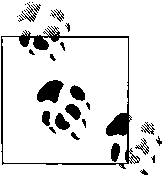
\includegraphics[width=2cm,clip]{paipai.png}
\end{wrapfigure}
\mbox{}\begin{flushleft}Unix系统为SIGCOUT定义了一个特例:在同一个会话中,进程可以给任何其它的进程发送该信号。用户ID不必相同。 \end{flushleft}

如果signo是0——前面提到过的空信号——调用不会发送信号,但是仍然进行错误检查。这对于测试一个进程是否有合适的权限给指定的进程发送信号时很有帮助。

\subsection{例子}

以下是如何给进程号为1722的进程发送SIGHUP的:

\begin{lstlisting}
int ret;
ret = kill (1722, SIGHUP);
if (ret)
    perror ("kill");
\end{lstlisting}

以上片段和下面执行的kill命令功能相同:

\begin{lstlisting}
$ kill -HUP 1722
\end{lstlisting}

检查我们是否有权限给1722进程发送信号,而实际上不发送任何信号,我们可以使用如下方式进行:

\begin{lstlisting}
int ret;
ret = kill (1722, 0);
if (ret)
    ; /* 我们没有权限 */
else
    ; /* 我们有权限 */
\end{lstlisting}

\subsection{给自己发送信号}

raise()函数是一种简单的进程给自己发送信号的方法:

\begin{lstlisting}
#include <signal.h>
int raise (int signo);
\end{lstlisting}

该调用:

\begin{lstlisting}
raise (signo);
\end{lstlisting}

和下面的调用是等价的:

\begin{lstlisting}
kill (getpid (), signo);
\end{lstlisting}

该调用成功时返回0,失败时返回非0值。它不设置errno。

\subsection{给整个进程组发送信号}

另一个非常方便的函数使得给特定进程组的所有进程发送信号变得非常简单,如果用进程组的ID的负值作为参数调用kill()就太麻烦了:

\begin{lstlisting}
#include <signal.h>
int killpg (int pgrp, int signo);
\end{lstlisting}

该调用:

\begin{lstlisting}
killpg (pgrp, signo);
\end{lstlisting}

和下面的调用等价:

\begin{lstlisting}
kill (-pgrp, signo);
\end{lstlisting}

即使pgrp是0,这也是正确的,在这种情况下,kill()给调用进程组的每个进程发送信号signo。

成功时,killpg()返回0,失败时,它返回-1,并将errno设置为以下之一:

\begin{eqlist*}
\item[EINVAL] 由signo指定的信号无效。
\item[EPERM] 调用进程缺乏足够的权限给指定进程发送信号。
\item[ESRCH] 由pgrp指定的进程组不存在。
\end{eqlist*}

\section{重入}

当内核发送信号时,进程可能执行到代码的任何位置。例如,进程可能正执行一个重要的操作,如果被中断,进程将会处于不一致的状态(例如数据结构只更新了一半,或计算只进行了一部分)。进程甚至可能正在处理另一个信号。

当信号到达时,信号处理程序不能说明进程正在执行什么代码;处理程序可以在任何情况下运行。因此任何该进程设置的信号处理程序都应该谨慎的对待它的操作和它涉及到的数据。信号处理程序必须注意,不要对进程被中断时正在做的事情做任何假设。尤其是当修改全局(也就是共享的)数据时必须要谨慎。总的来说,信号处理程序从不接触全局数据是一个比较好的选择;在接下来的部分,我们会看一种暂时阻止接收信号的方法,从而提供一种处理信号处理程序和进程其它部分共享数据的安全操作方法。

系统调用和其它库函数又是什么情况呢?如果你的进程正在写文件或申请内存中,信号处理程序向同一个文件写入或也在调用malloc()会怎么样?或者当信号被发送时,进程正在调用一个使用静态缓存的函数,例如strsignal(),情况又会是什么样?

一些函数显然是不可重入的。如果程序正在执行一个不可重入的函数中,信号发生了,信号处理程序调用同样的不可重入的函数,那么就会造成混乱。可重入函数是指可以安全的调用自身(或者从同一个进程的另一个线程)的函数。为了使函数可重入,函数决不能操作静态数据,必须只操作栈分配的数据或调用者提供的数据,不得调用任何不可重入的函数。

\subsection{有保证的可重入函数}

当写信号处理程序时,你必须假设中断的进程可能处于不可重入的函数中(就此而言,或其它的东西)。因此,信号处理程序必须只使用可重入函数。

各种标准已经颁布了信号安全(即可重入)的函数清单,因此可在信号处理程序中安全的使用。最值得注意的是POSIX.1-2003和Unix信号规范,它们规定了在所有标准平台上都保证可重入和信号安全函数的清单。表9-2列出了这些函数。

表9-2 可在信号中安全使用的确保可重入的函数

\begin{tabular}{l l l}
abort() & accept() & access()\\
aio\_error() & aio\_return() & aio\_suspend()\\
alarm() & bind() & cfgetispeed()\\
cfgetospeed() & cfsetispeed() & cfsetospeed()\\
chdir() & chmod() & chown()\\
clock\_gettime() & close() & connect()\\
creat() & dup() & dup2()\\
execle() & execve() & Exit()\\
\_exit() & fchmod() & fchown()\\
fcntl() & fdatasync() & fork()\\
fpathconf() & fstat() & fsync()\\
ftruncate() & getegid() & geteuid()\\
getgid() & getgroups() & getpeername()\\
getpgrp() & getpid() & getppid()\\
getsockname() & getsockopt() & getuid()\\
kill() & link() & listen()\\
lseek() & lstat() & mkdir()\\
mkfifo() & open() & pathconf()\\
pause() & pipe() & poll()\\
posix\_trace\_event() & pselect() & raise()\\
read() & readlink() & recv()\\
recvfrom() & recvmsg() & rename()\\
rmdir() & select() & sem\_post()\\
send() & sendmsg() & sendto()\\
setgid() & setpgid() & setsid()\\
setsockopt() & setuid() & shutdown()\\
sigaction() & sigaddset() & sigdelset()\\
sigemptyset() & sigfillset() & sigismember()\\
signal() & sigpause() & sigpending()\\
sigprocmask() & sigqueue() & sigset()\\
sigsuspend() & sleep() & socket()\\
socketpair() & stat() & symlink()\\
sysconf() & tcdrain() & tcflow()\\
tcflush() & tcgetattr() & tcgetpgrp()\\
tcsendbreak() & tcsetattr() & tcsetpgrp()\\
time() & timer\_getoverrun() & timer\_gettime()\\
timer\_settime() & times() & umask()\\
uname() & unlink() & utime()\\
wait() & waitpid() & write()\\
\end{tabular}

有更多的函数是安全的,但是Linux和其它POSIX标准的系统只保证这些函数是可重入的。

\section{信号集}

我们将在本章稍后提到的一些函数需要操作信号集,例如被一个进程阻塞的信号的集合,或者待处理的信号集合。以下列出的信号集合操作可以管理这些信号集:

\begin{lstlisting}
#include <signal.h>
int sigemptyset (sigset_t *set);
int sigfillset (sigset_t *set);
int sigaddset (sigset_t *set, int signo);
int sigdelset (sigset_t *set, int signo);
int sigismember (const sigset_t *set, int signo);
\end{lstlisting}

sigemptyset()初始化由set给定的信号集,将集合标记为空(所有的信号都被排除在集合外)。sigfillset()初始化由set给定的信号集,将它标记为满(所有的信号都包括在集合内)。两个函数都返回0。你应该在使用信号集之前调用这两个函数之一。

sigaddset()将signo加入到set给定的信号集中,sigdelset()将signo从set给定的信号集中删除。成功时两者都返回0,错误时都返回-1,在这种情况下errno被设置成EINVAL,这意味着signo是一个无效的信号标识符。

如果signo在由set指定的信号集中,sigismember()返回1,如果不在则返回0,错误时返回-1。在后一种情况下errno被设置为EINVA,意味着signo无效。

\subsection{更多的信号集函数}

上述的函数都是由POSIX标准定义的,可以在任何现代的Unix系统中找到。Linux也提供了一些非标准的函数:

\begin{lstlisting}
#define _GNU_SOURCE
#define <signal.h>
int sigisemptyset (sigset_t *set);
int sigorset (sigset_t *dest, sigset_t *left, sigset_t *right);
int sigandset (sigset_t *dest, sigset_t *left, sigset_t *right);
\end{lstlisting}

如果由set给定的信号集是空的sigisemptyset()返回1,否则返回0。

sigorset()将信号集left和right的并(二进制或)赋给dest。sigandset()将信号集left和right的交(二进制与)赋给dest。成功时两者都返回0,错误时返回-1,并将errno设置为EINVAL。

这些函数是有用的,但是希望完全符合POSIX标准的程序应该避免使用它们。

\section{阻塞信号}

前面我们讨论了重入和由信号处理程序异步运行引发的问题。我们讨论了不能从信号处理程序内部调用的函数,因为它们是不可重入的。

但是如果你的程序需要在信号处理程序和程序其它部分共享数据时该怎么办?如果你程序中的某些部分在运行期间不希望被中断(包括来自信号处理程序的中断)时该怎么办?我们把这些部分叫做临界区,我们通过临时挂起信号来保护它们。我们称这些信号被阻塞。任何被挂起的信号都不会被处理,直到它们被解除阻塞。进程可以阻塞任意多个信号;被进程阻塞的信号叫做该进程的信号掩码。POSIX定义,Linux实现了一个管理进程信号掩码的函数:

\begin{lstlisting}
#include <signal.h>
int sigprocmask (int how,
                 const sigset_t *set,
                 sigset_t *oldset);
\end{lstlisting}

sigprocmask()的行为取决于how的值,它是以下标识之一:

\begin{eqlist*}
\item[SIG\_SETMASK] 调用进程的信号掩码变成set。
\item[SIG\_BLOCK] set中的信号被加入到调用进程的信号掩码中。也就是说,信号掩码变成了当前信号掩码和set的并集(二进制或)。
\item[SIG\_UNBLOCK] set中的信号被从调用进程的信号掩码中移除。也就是说,信号掩码变成了当前信号掩码和set补集(二进制非)的交集(二进制与)。将一个未阻塞的信号解除阻塞是非法的。
\end{eqlist*}

如果oldset是非空的,该函数将oldset设置为先前的信号集。

如果set是空的,该函数会忽略how,并且不改变信号掩码,但仍然设置oldset的信号掩码。换句话说,给set一个空值是检测当前信号掩码的一种方法。

 调用成功,返回0。失败时返回-1,把errno设置为EINVAL,表示how是无效的,或者设置为EFAULT,表示set或oldset是无效指针。

阻塞SIGKILL或SIGSTOP是不允许的。sigprocmask()会悄悄的忽略任何将这两个信号加入信号掩码的尝试。

\subsection{获取待处理信号}

当内核产生一个被阻塞的信号时,该信号未被发送。我们把它叫做待处理信号。当一个待处理信号解除阻塞时,内核会把它发送给进程处理。

POSIX定义了一个检测待处理信号集的函数:

\begin{lstlisting}
#include <signal.h>
int sigpending (sigset_t *set);
\end{lstlisting}

成功的调用sigpending()会将set设置为待处理的信号集,并返回0。失败时,该调用返回-1,并将errno设置成EFAULT,意味着set是一个无效指针。

\subsection{等待信号集}

下面是第三个POSIX定义的允许进程临时改变信号掩码的函数,该函数始终出于等待状态,直到产生一个终止该进程或被该进程处理的信号:

\begin{lstlisting}
#include <signal.h>
int sigsuspend (const sigset_t *set);
\end{lstlisting}

如果一个信号终止了进程,sigsuspend()不返回。如果一个信号被发送和处理了,sigsuspend()在信号处理程序返回后,返回-1并将errno设置为EINTR。如果set是一个无效指针,errno被设置成EFAULT。

一般在获取已达到信号和在程序运行期间阻塞在临界区的信号时使用sigsuspend()。进程首先使用sigprocmask()来阻塞一个信号集,将旧的信号掩码保存在oldset中。退出临界区后,进程会调用sigsuspend(),将oldset赋给set。

\section{高级信号管理}

我们在本章开头学习的signal()函数是非常基本的。它是C标准库的一部分,因此必须考虑对它运行的操作系统能力做最小的假设,它只提供了最低限度的信号管理的标准。作为另一种选择,POSIX定义了sigaction()系统调用,它提供了更加强大的信号管理能力。除此之外,当信号处理程序运行时,你可以用它来阻塞特定信号的接收,你也可以用它来获取信号发送时各种操作系统和进程状态的信息:

\begin{lstlisting}
#include <signal.h>
int sigaction (int signo,
               const struct sigaction *act,
               struct sigaction *oldact);
\end{lstlisting}

调用sigaction()会改变由signo表示的信号的行为,signo可以是除了SIGKILL和SIGSTOP外的任何值。如果act是非空的,该系统调用将该信号的当前行为替换成由act指定的行为。如果oldact是非空的,该调用会存储先前(或者是当前的,如果act是非空的)给定的信号行为。

sigaction结构允许精细的控制信号。头文件<sys/signal.h>包含<signal.h>以如下形式定义该结构

\begin{lstlisting}
struct sigaction {
    void (*sa_handler)(int);   /* 信号处理程序或操作 */
    void (*sa_sigaction)(int, siginfo_t *, void *);
    sigset_t sa_mask;          /* 阻塞的信号 */
    int sa_flags;              /* 标志 */
    void (*sa_restorer)(void); /* 已经过时且不符合 POSIX 标准 */
}
\end{lstlisting}

sa\_handler域规定了接收信号时采取的操作。对于signal()来说,该域可能是SIG\_DFL,表示默认操作,可能是SIG\_IGN,指示内核忽略该信号,或者是一个指向信号处理函数的指针。该函数和signal()安装的信号处理程序具有相同的原型:

\begin{lstlisting}
void my_handler (int signo);
\end{lstlisting}

如果sa\_flags被置成SA\_SIGINFO,那么将由sa\_sigaction而不是sa\_handle指示信号处理函数。该函数的原型略有不同:

\begin{lstlisting}
void my_handler (int signo, siginfo_t *si, void *ucontext);
\end{lstlisting}

该函数接受信号编号作为它的第一个参数,siginfo\_t结构作为第二个参数,ucontext\_t结构(强转成void指针)作为第三个参数。它没有返回值。siginfo\_t结构给信号处理程序提供了丰富的信息;我们很快就会看到它。

请注意,在一些机器结构中(可能是其它的Unix系统),sa\_handler和sa\_sigaction是在一个联合中,因此你不能给两个域同时赋值。

sa\_mask域提供了应该在执行信号处理程序时被阻塞的信号集。这使得程序员为多个信号处理程序间的重入提供适当的保护。当前正在处理的信号也是被阻塞的,除非将sa\_flags设置成了SA\_NODEFER标志。不可以阻塞SIGKILL或SIGSTIO;该调用会在sa\_mask中悄悄的忽略它们。

sa\_flag域是零,一或更多改变signo表示信号的标志的位掩码。我们已经看过了SA\_SIGINFO和SA\_NODEFER标志,sa\_flags的其它值包括以下几个:

\begin{eqlist*}
\item[SA\_NOCLDSTOP] 如果signo是SIGCHLD,该标志指示系统在子进程停止或继续执行时不要提供通知。
\item[SA\_NOCLDWAIT] 如果signo是SIGCHLD,该标志可以自动获取子进程:子进程结束时不会变成僵尸进程,父进程不需要(并且也不能)为子进程调用wait()。见第五章对子进程,僵尸进程和wait()的讨论。
\item[SA\_NOMASK] 该标志已过时且不符合POSIX标准,该标志与SA\_NODEFER等价(此部分前面讨论过)。使用SA\_NODEFER代替该标志,但是在一些旧的代码中还能见到该标志。
\item[SA\_ONESHOT] 该标志已过时且不符合POSIX标准,该标志与SA\_NODEFER等价(在下文会讨论)。使用SA\_NODEFER代替该标志,但是在一些旧的代码中还能见到该标志。
\item[SA\_ONSTACK] 该标志指示系统在一个替代的信号栈中调用给定的信号处理程序,该信号栈是由sigaltstack()提供的。如果你没提供一个替代的栈,系统会使用默认的栈,也就是说,系统的行为和未提供该标志一样。替代的信号栈是很罕见的,虽然它们在一些较小线程栈的pthreads应用程序中是有用的,这些线程栈在被一些信号处理程序使用时可能会溢出。在本书中我们不再进一步讨论sigaltstack()。
\item[SA\_RESTART] 该标志可以使被信号中断的系统调用以BSD风格重新启动。
\item[SA\_RESETHAND] 该标志表示“一次性”模式。一旦信号处理程序返回,给定信号会被重设为默认操作。
\end{eqlist*}

sa\_restorer域是过时的,并且也不在Linux中使用。它不是POSIX的一部分。假装它不存在,不必去管它。

成功时sigaction()返回0。失败时,该调用返回-1,并将errno设置为以下错误代码之一:

\begin{eqlist*}
\item[EFAULT] act或oldact是无效指针。
\item[EINVAL] signo是无效的信号,SIGKILL或SIGSTOP。
\end{eqlist*}
\subsection{siginfo\_t结构}

siginfo\_t结构也是在<sys/signal.h>中定义的,如下:

\begin{lstlisting}
typedef struct siginfo_t {
    int si_signo;      /* 信号编号 */
    int si_errno;      /* errno 值 */
    int si_code;       /* 信号代码 */
    pid_t si_pid;      /* 发送进程的PID */
    uid_t si_uid;      /* 发送进程的真实UID */
    int si_status;     /* 退出值或信号 */
    clock_t si_utime;  /* 用户时间消耗 */
    clock_t si_stime;  /* 系统时间消耗 */
    sigval_t si_value; /* 信号载荷值 */
    int si_int;        /* POSIX.1b 信号 */
    void *si_ptr;      /* POSIX.1b 信号 */
    void *si_addr;     /* 造成错误的内存位置 */
    int si_band;       /* 带事件 */
    int si_fd;         /* 文件描述符 */
};
\end{lstlisting}

这种结构中都是传递给信号处理程序的信息(如果你使用sa\_sigaction代替sa\_sighandler)。在现代计算技术中,许多人认为Unix信号模型是一种非常糟糕的实现IPC(进程间通信)的方法。这很有可能是因为当他们应该使用sigaction()和SA\_SIGINFO时,这些人仍然坚持使用signal()。siginfo\_t结构为我们打开了方便之门,在信号之上又衍生了大量的功能。

在该结构中有许多有趣的数据,包括发送信号进程的信息,以及信号产生的原因。以下是对每个域的详细描述:

\begin{eqlist*}
\item[si\_signo] 信号的编号。在你的信号处理程序中,第一个参数也提供了该信息(避免使用一个复引用的指针)。
\item[si\_errno] 如果是非零值,表示与该信号有关的错误代码。该域对所有的信号都有效。
\item[si\_code] 解释进程为什么收到信号以及信号由哪(例如,来自kill())发出。我们会在下一部分浏览一下可能的值。该域对所有的信号都有效。
\item[si\_pid] 对于SIGCHLD,表示终止进程的PID。
\item[si\_uid] 对于SIGCHLD,表示终止进程自己的UID。
\item[si\_status] 对于SIGCHLD,表示终止进程的退出状态。
\item[si\_utime] 对于SIGCHLD,表示终止进程消耗的用户时间。
\item[si\_stime] 对于SIGCHLD,表示终止进程消耗的系统时间。
\item[si\_value] si\_int和si\_ptr的联合。
\item[si\_int] 对于通过sigqueue()发送的信号(见本章稍后的“发送带附加信息的信号”),以整数类型作为参数。
\item[si\_ptr] 对于通过sigqueue()发送的信号(见本章稍后的“发送带附加信息的信号”),以void指针类型作为参数。
\item[si\_addr] 对于SIGBUS,SIGFPE,SIGILL,SIGSEGV和SIGTRAP,该void指针包含了引发错误的地址。例如对于SIGSEGV,该域包含非法访问内存的地址(因此常常是NULL)。
\item[si\_band] 对于SIGPOLL,表示si\_fd中列出的文件描述符的带外和优先级信息。
\item[si\_fd] 对于SIGPOLL,表示操作完成的文件的描述符。
\end{eqlist*}

si\_value,si\_int和si\_ptr是相对复杂的部分,因为进程可以用它们给另一个进程传递任何数据。因此,你可以用它们发送一个整数或一个指向数据结构的指针(注意,如果进程不共享地址空间,那么指针是没有用的)。在接下来的“发送带附加信息的信号”部分会讨论这些域。

POSIX只保证前三个域是对于所有信号都有效的。其它的域只有在处理相应的信号时才被访问。例如,只有信号是SIGPOLL时,你才应该访问si\_fd域。

\subsection{si\_code的精彩世界}

si\_code域说明信号发生的原因。对于用户发送的信号,该域说明信号是如何被发送的。对于内核发送的信号,该域说明信号发送的原因。

以下的si\_code值对任何信号都是有效的。它们说明了信号如何/为什么被发送。

\begin{eqlist*}
\item[SI\_ASYNCIO] 由于完成异步I/O而发送该信号(见第五章)。
\item[SI\_KERNEL] 信号由内核产生。
\item[SI\_MESGQ] 由于一个POSIX消息队列的状态该变而发送该信号(不在本书的范围内)。
\item[SI\_QUEUE] 信号由sigqueue()发送(见下一部分)。
\item[SI\_TIMER] 由于POSIX定时器超时而发送该信号(见第十章)。
\item[SI\_TKILL] 信号由tkill()或tgkill()发送。这些系统调用是线程库使用的,不在本书的讨论范围内。
\item[SI\_SIGIO] 由于SIGIO排队而发送该信号。
\item[SI\_USER] 信号由kill()或raise()发送。
\end{eqlist*}

以下的si\_code值只对SIGBUS有效。它们说明了发生硬件错误的类型:

\begin{eqlist*}
\item[BUS\_ADRALN] 进程发生了对齐错误(间第八章对对齐的讨论)。
\item[BUS\_ADRERR] 进程访问无效的物理地址。
\item[BUS\_OBJERR] 进程造成了其它类型的硬件错误。
\end{eqlist*}

 对于SIGCHLD,以下的值表示子进程给父进程发送信号时的行为:

\begin{eqlist*}
\item[CLD\_CONTINUED] 子进程被停止,但已经继续执行。
\item[CLD\_DUMPED] 子进程非正常终止。
\item[CLD\_EXITED] 子进程通过exit()正常终止。
\item[CLD\_KILLED] 子进程被杀死了。
\item[CLD\_STOPPED] 子进程被停止了。
\item[CLD\_TRAPPED] 子进程进入一个陷井。
\end{eqlist*}

以下的值只对SIGFPE有效。它们说明了发生算术错误的类型:

\begin{eqlist*}
\item[FPE\_FLTDIV] 进程执行了一个除以0的浮点数运算。
\item[FPE\_FLTOVF] 进程执行了一个溢出的浮点数运算。
\item[FPE\_FLTINV] 进程执行了一个无效的浮点数运算。
\item[FPE\_FLTRES] 进程执行了一个不精确或无效结果的浮点数运算。
\item[FPE\_FLTSUB] 进程执行了一个造成下标超出范围的浮点数运算。
\item[FPE\_FLTUND] 进程执行了一个造成下溢的浮点数运算。
\item[FPE\_INTDIV] 进程执行了一个除以0的整数运算。
\item[FPE\_INTOVF] 进程执行了一个溢出的整数运算。
\item[FPE\_FLTDIV] 进程执行了一个除以0的浮点数运算。
\item[FPE\_FLTOVF] 进程执行了一个溢出的浮点数运算。
\item[FPE\_FLTINV] 进程执行了一个无效的浮点数运算。
\item[FPE\_FLTRES] 进程执行了一个不精确或无效结果的浮点数运算。
\item[FPE\_FLTSUB] 进程执行了一个造成下标超出范围的浮点数运算。
\item[FPE\_FLTUND] 进程执行了一个造成下溢的浮点数运算。
\item[FPE\_INTDIV] 进程执行了一个除以0的整数运算。
\item[FPE\_INTOVF] 进程执行了一个溢出的整数运算。
\end{eqlist*}

以下si\_code值只对SIGILL有效。它们说明了执行非法指令的性质:

\begin{eqlist*}
\item[ILL\_ILLADR] 进程试图进入非法的寻址模式。
\item[ILL\_ILLOPC] 进程试图执行一个非法的操作码。
\item[ILL\_ILLOPN] 进程试图执行一个非法的操作数。
\item[ILL\_PRVOPC] 进程试图执行特权操作码。
\item[ILL\_PRVREG] 进程试图在特权寄存器上运行。
\item[ILL\_ILLTRP] 进程试图进入一个非法的陷井。
\end{eqlist*}

对于所有的这些值,si\_addr都指向非法操作的地址。

对于SIGPOLL,以下的值表明标识形成信号的I/O事件:

\begin{eqlist*}
\item[POLL\_ERR] 发生了I/O错误。
\item[POLL\_HUP] 设备挂起或套接字断开。
\item[POLL\_IN] 文件有可读数据。
\item[POLL\_MSG] 有一个消息。
\item[POLL\_OUT] 文件能够被写入。
\item[POLL\_PRI] 文件有可读的高优先级数据。
\end{eqlist*}

以下的代码对SIGSEGV有效,描述了两种非法访存的类型:

\begin{eqlist*}
\item[SEGV\_ACCERR] 进程以无效的方式访问有效的内存区域,也就是说进程违反了内存访问的权限。
\item[SEGV\_MAPERR] 进程访问无效的内存区域。
\end{eqlist*}

对于这两个值,si\_addr包含了非法操作的地址。

对于SIGTRAP,这两个si\_code值标识了进入陷井的类型:

\begin{eqlist*}
\item[TRAP\_BRKPT] 进程进入一个断点。
\item[TRAP\_TRACE] 进程进入了一个追踪陷井。
\end{eqlist*}

注意,si\_code是一个数值域,而不是一个位域。

\section{发送带附加信息的信号}

正如我们前面部分看到的,以SA\_SIGINFO标志注册的信号处理程序传递了一个siginfo\_t参数。该结构包含了一个名为si\_value的域,该域可以让信号产生者向信号接受者传递一些附加信息。

由POSIX定义的sigqueue()函数,允许进程发送带附加信息的信号:

\begin{lstlisting}
#include <signal.h>
int sigqueue (pid_t pid,
              int signo,
              const union sigval value);
\end{lstlisting}

sigqueue()和kill()的运行方式很像。成功时,由signo表示的信号被加入到由pid指定的进程或进程组的队列中,并返回0。信号的载荷是由数值给定的,它是一个整数和void指针的联合:

\begin{lstlisting}
union sigval {
    int sival_int;
    void *sival_ptr;
};
\end{lstlisting}

失败时,该调用返回-1,并将errno设置为以下之一:

\begin{eqlist*}
\item[EINVAL] 由signo指定的信号无效。
\item[EPERM] 调用进程缺乏足够的权限给任何指定的进程发送信号。发送信号的权限要求和kill()是一样的(见本章前面的“发送信号”部分)。
\item[ESRCH] 由pid指定的进程或进程组不存在,或者进程是一个僵尸进程。
\end{eqlist*}

\subsection{例子}

这个例子是给pid为1722的进程发送一个附加为整数值的SIGUSR2信号,其值为404:

\begin{lstlisting}
sigval value;
int ret;
value.sival_int = 404;
ret = sigqueue (1722, SIGUSR2, value);
if (ret)
    perror ("sigqueue");
\end{lstlisting}

如果1722进程用SA\_SIGINFO处理程序处理SIGUSR2,它会发现signo被设成了SIGUSR2,si->si\_int被设成了404,si->si\_code被设成了SI\_QUEUE。

\section{结论}

信号在很多Unix程序员中的名声很坏。它们是古老且过时的内核与用户间的通讯机制,顶多能算是一种原始的进程间通信机制。在多线程程序和循环事件中,信号往往是不合适的。

然而,不管是好是坏,我们还需要它们。信号是从内核接收许多通知(例如通知进程执行了非法的操作码)的唯一方式。此外,信号还是Unix(Linux也一样)终止进程和管理父/子进程关系的方式。因此,我们坚持使用它们。

批评信号的主要理由之一是,很难写出一个安全的可重入的信号处理程序。如果你能简化你的信号处理程序,并且只使用表9-2列出的函数(你可以用任意多个!),它们就应该是安全的。

另一个信号外在的不足是,许多程序员仍然使用signal()和kill()而不是sigaction()和sigqueue()来管理信号。正如最后两小节表明的,当使用SA\_SIGINFO风格的处理程序时,信号的健壮性和表达力会显著增强。尽管我本人不喜欢信号(我希望看到信号被一个基于文件描述符的可修改的机制取代,这实际上是未来Linux内核版本正在考虑的事)绕过它们的缺陷并使用Linux的高级信号接口,确实可以避免大多数的麻烦(如果不是发牢骚)。

\ifx\atempxetex\usewhat
\XeTeXinputencoding "utf-8"
\fi
\defaultfont

\chapter{时间}

时间在现代操作系统中有许多用途,许多程序都需要追踪它。内核从三个角度来度量时间:

\textit{墙上时间(或真实时间)}

这是真实世界中的实际时间和日期——就是说,是墙上挂钟的时间。进程在与用户交互以及为事件标记时间戳时使用墙上时间。

\textit{进程时间}

即进程消耗的时间,包括用户空间代码直接使用的时间和在内核在该进程上消耗的时间。进程通常在对程序进行剖析和统计时使用它(例如,来衡量一个操作耗时多少)。因为Linux是多任务的,在度量进程行为时使用墙上时间容易产生误导,一个操作的进程时间可能比墙上时间少许多。进程也会消耗掉相当多个时钟周期去等待I/O(尤其是键盘输入)。

\textit{单调时间}

这个时间源是严格线性增长的。包括Linux在内的大多数操作系统,使用计算机的正常运行时间(系统已启动的时间)。墙上时间可能会发生变化(例如用户可以进行设定或系统会由于误差不断调校这个时间),也会引入某些不精确性,例如闰秒。系统正常运行时间,从另一方面来说,是一种确定的不可改变的时间表示方法。单调时间源的重要性不在于当前值,而是可以保证时间源线性增长,并利用该特性来计算两次时间采样的差值。

因而单调时间适合来计算相对时间,而墙上时间对于衡量绝对时间更为理想。

这三种时间测量方法可以用以下两种形式来表现: 

\textit{相对时间}

这是相对于某个基准时间(例如当前时刻)的值:举个例子,从现在起5秒钟,或者10分钟之前。

\textit{绝对时间}

表示不含任何基准的时间,例如1968年3月25日中午。 

相对和绝对两种时间形式都是有用的。一个进程可能需要在500毫秒内取消一个请求,每秒刷新60次屏幕,或者记录某操作开始后已经过去了7秒。所有这些都需计算相对时间。反过来,一个日历应用可能要保存用户聚会日期为2月8日,一个文件系统将在某个文件创建时写入完整的日期和时间(而不是“5秒前” 这样的相对时间),用户的时钟显示公历日期,不是自系统启动后的相对时间。

Unix系统使用从大纪元——定义为1970年1月1日00:00:00——以来经过的秒数来表示绝对时间。UTC(协调世界时)差不多就是GMT(格林尼治标准时间)或祖鲁时间。有意思的是,这意味着在Unix中即便是绝对时间本身,从更底层来讲也是相对的。Unix引入了一种特殊的数据类型来存储“自从大纪元以来流逝的秒数”,我们将在下一节探讨。

软件时钟是由内核维护的时钟,操作系统通过软件时钟来追踪时间进程。内核初始化一个遵循特定频率的周期计时器,一般被称为系统计时器 (system timer)。当一个计时器间隔结束时,内核将消耗时间值增加一个单位,记做一个tick 或者 jiffy。记录jiffy数量的计数器被称作jiffy计数器(jiffies counter)。jiffy以前是32位值,在2.6 Linux内核后则使用64位值进行计数。\footnote[1]{Linux内核的未来版本可能会是“无时钟报时”或者会实现“动态时钟报时”,即内核不会记录一个显式jiffy值。这样所有基于时间的内核操作将伴随动态建立的计时器执行,而不是系统计时器。}

Linux中的系统计时器频率被称为HZ,因为有个同样名字的宏被定义来指称这个概念。HZ的值是体系结构相关的,并且不是 Linux ABI的一部分——就是说,程序不能依赖于,也不能期望它等于某个特定值。历史上,x86架构定义该值为100,表示系统计时器每秒钟运行100次(就是说系统计时器的频率是100HZ)。这就使每个jiffy的值为0.01秒——1/HZ秒。在2.6 Linux内核中,内核开发者把HZ的值一下子提升到1000,使得每个jiffy的值变成0.001秒。然而,在2.6.13和之后的版本中,HZ是 250,每个jiffy为0.004秒。\footnote[1]{HZ现在是内核编译期的可选项,在x86架构上值可以是100、250和1000。与此无关的是,用户空间不能依赖于任何特定的HZ值。}在HZ的值的选择上需要加以权衡:较高的值能提供较高的精度,但带来了更大的计时器开销。

尽管进程不应依赖于任何确定的HZ值,POSIX定义了一种在运行时确定系统计时器频率的机制: 

\begin{lstlisting}
  long hz;

  hz = sysconf (_SC_CLK_TCK);
  if (hz ==  -1)
  	perror (``sysconf''); /* should never occur */
\end{lstlisting}
  
当一个程序想要确定系统计时器频率的时候,这个函数很有帮助,但将系统时间转换到秒就没有必要使用它了,因为大多数POSIX函数输出的时间测量结果已经被转换或者缩放至一个与HZ无关的确定值。与HZ不同的是,这个固定的频率是系统ABI的一部分;在x86上的值是100。以系统时钟周期数做为返回值的 POSIX函数用CLOCKS\_PER\_SEC来表示该固定的频率。

偶尔,一些突发事件会导致计算机意外关闭。有时计算机甚至会被断电;然而到启动时,时间仍然正确无误。这是因为大多数计算机都有一个电池供电的硬件时钟在其关闭时存储时间和日期。当内核启动时,就从该硬件时钟来初始化当前时间。同样,当用户关闭计算机时,内核将时间写回到硬件时钟里。系统管理员可以通过hwclock命令将时钟更新为其他时间。

管理Unix系统的时间包括几个任务,其中只有一部分是所有进程都需要关心的,其中包括设定和取得当前墙上时间,计算消耗时间,睡眠一段时间,进行精确的时间测量,以及控制定时器。本章涵盖了时间相关的所有内容。我们将从Linux表示时间的数据结构开始看起。 

\section{时间的数据结构}

随着各种Unix系统的发展,它们用多种数据结构来表示看似简单的时间概念,并在此基础上实现了各自的时间管理函数。这些数据结构可以说是花样繁多,既有简单的整型,也有多字段结构体。在我们深入函数细节之前,我们先来讨论一下这些数据结构。 

\subsection{原始表示}

最简单的数据结构是time\_t,定义在头文件<time.h>中。time\_t意图成为隐晦的类型。然而,在大多数Unix系统上(包括Linux)这个类型是一个简单的C语言的长整型: 

\begin{lstlisting}
  typedef long time_t;
\end{lstlisting}

time\_t表示自大纪元以来已流逝的秒数。对此人们典型的反应是“那岂不是过不了多久就会溢出!”。实际上,会比你想的要久一些,但在大量目前仍然在使用的Unix系统中确实会出现溢出。使用32位的长整型,time\_t最多能表示大纪元后2,147,483,647秒。这表示我们将会在2038年再一次遭遇千年虫!然而幸运的是,在2038年一月18日,星期一的22:14:07时,大多数系统和软件将会是64位的。

\subsection{微秒级精度}

与time\_t相关的另外一个问题是一秒钟内会发生很多事情。timeval结构对time\_t进行了扩展而达到了微秒级精度。头文件<sys/time.h>对其定义如下: 

\begin{lstlisting}
  #include <sys/time.h>

  struct timeval {
      time_t tv_sec; /* seconds */
      suseconds_t tv_usec; /* microseconds */
  };  
\end{lstlisting}

tv\_sec衡量秒数,而tv\_usec衡量毫秒数。令人困惑的suseconds\_t通常是一个整型的typedef。 

\subsection{纳秒级精度}

出于对毫秒级精度的不满,timespec结构将精度提高到了纳秒级。头文件<time.h>对其定义如下: 

\begin{lstlisting}
  #include <time.h>

  struct timespec {
      time_t tv_sec; /* seconds */
      long tv_nsec; /* nanoseconds */
  };
\end{lstlisting}

如果有选择,函数会更愿意采用纳秒级精度而非毫秒级。因此,引入timespec结构后,大多数时间相关的函数就采用了它,并获得了更高的精度。然而,正如我们将看到的,一个重要的函数仍然使用timeval。

在实践中,因为系统计时器没有提供纳秒级甚至毫秒级的精度,没有任何一个这里所提到的结构能够提供其所声明的精度。不过,函数中尽量采用可用的高精度是较好的选择,因为这样就可以利用系统所提供的各种精度。

\subsection{“分解”时间}

我们将要讨论的一些函数经常需要进行Unix时间与字符串之间的转换,或者构建一个字符串来表示时间。为了简化该过程,标准C提供了结构体tm,将Unix时间拆分为人们容易理解的格式。这个结构也定义在<time.h>中: 

\begin{lstlisting}
  #include <time.h>

  struct tm {
      int tm_sec; /* seconds */
      int tm_min; /* minutes */
      int tm_hour; /* hours */
      int tm_mday; /* the day of the month */
      int tm_mon; /* the month */
      int tm_year; /* the year */
      int tm_wday; /* the day of the week */
      int tm_yday; /* the day in the year */
      int tm_isdst; /* daylight savings time? */
  #ifdef _BSD_SOURCE
      long tm_gmtoff; /* time zone's offset from GMT */
      const char *tm_zone; /* time zone abbreviation */
  #endif /* _BSD_SOURCE */
  };
\end{lstlisting}

tm结构体可以让我们更容易的理解time\_t的值代表什么,比如说,314159是周日还是周六(应该是前者)。从占用空间的角度来看,这样表示日期时间显然是一个糟糕的选择,但使用这种表示来转换面向用户的值时却更加方便。

tm结构体有如下这些字段: 

\begin{eqlist*}
\item [tm\_sec]
在分钟后的秒数。这个值通常在0到59之间,但也可以达到61来表示最多2个闰秒。
\item [tm\_min]
小时后的分钟数。这个值在0到59之间。 
\item [tm\_hour]
午夜过后的小时数。这个值在0到23之间。 
\item [tm\_mday]
该月的日期。这个值在0到31之间。POSIX并没有指定0值;然而,Linux用它表示上个月的最后一天。 
\item [tm\_mon]
从一月以来的月数。这个值在0到11之间。
\item [tm\_year]
从1900年以来的年数。
\item [tm\_wday]
从周日以来的天数。这个值在0到6之间。
\item [tm\_yday]
从一月1日以来的日期数。这个值在0到365之间。
\item [tm\_isdst]
这个值用来表示夏令时(DST)在其他字段描述的时间是否有效。如果这个值为正,那么DST有效。如果是0,DST无效。如果是负数,DST的状态未知。
\item [tm\_gmtoff]
以秒计的当前时区与格林尼治时间偏差值。这个字段仅仅在包含<time.h>之前定义了\_BSD\_SOURCE才会出现。
\item [tm\_zone]
当前时区的缩写——例如EST。这个字段仅仅在包含<time.h>之前定义了\_BSD\_SOURCE才会出现。 
\end{eqlist*}

\subsection{一种进程时间类型}

clock\_t类型表示时钟“滴答”数。这是个整数类型,通常是长整型。对于不同函数,clock\_t表示系统实际计时器频率(HZ)或者CLOCKS\_PER\_SEC。

\section{POSIX时钟}

本章讨论的一些系统调用使用了POSIX时钟,它是一种实现和表示时间源的标准。clockid\_t类型表示了特定的POSIX时钟,Linux支持其中四种:

\begin{eqlist*}
\item [CLOCK\_MONOTONIC]
一个不可被任何进程设置的单调增长的时钟。它表示自某个非特定起始点以来流逝的时间,例如从系统启动开始。
\item [CLOCK\_PROCESS\_CPUTIME\_ID]
一个处理器提供给每个进程的高精度时钟。例如,在i386架构上,这个时钟采用时间戳计数(TSC)寄存器。
\item [CLOCK\_REALTIME]
系统级真实时间(墙上时间)时钟。设置该时钟需要特殊权限。
\item [CLOCK\_THREAD\_CPUTIME\_ID]
和每个进程的时钟类似,但是是线程独有的。
\end{eqlist*}
POSIX定义了所有四个时间源,但只有CLOCK\_REALTIME是必须实现的。因而,虽然Linux提供了所有四个时钟,但可移植的代码应该仅仅使用CLOCK\_REALTIME。 

\section{时间源精度}

POSIX定义了clock\_getres()函数来取得给定时间源的精度。

\begin{lstlisting}
  #include <time.h>

  int clock_getres (clockid_t clock_id,
                    struct timespec *res);
\end{lstlisting}
成功调用clock\_getres()会将clock\_id指定的时钟精度存储到res中,如果结果不是NULL,就返回0。失败时,函数返回-1,并设置errno为以下两个错误码>之一:

\begin{eqlist*}
\item [EFAULT]
res是一个非法的指针。 
\item [EINVAL]
clock\_id在该系统上不是一个可用的时间源。 
\end{eqlist*}

以下的示例代码将输出先前讨论的四种时间源的精度:

\begin{lstlisting}
  clockid_t clocks[] = {
          CLOCK_REALTIME,
          CLOCK_MONOTONIC,
          CLOCK_PROCESS_CPUTIME_ID,
          CLOCK_THREAD_CPUTIME_ID,
	  (clockid_t) -1 };
  int i;

  for (i = 0; clocks[i] != (clockid_t) -1; i++) {
      struct timespec res;
      int ret;

      ret = clock_getres (clocks[i], &res);
      if (ret)
	  perror (``clock_getres'');
      else
	  printf (``clock=%d sec=%ld nsec=%ld\n'',
  clocks[i], res.tv_sec, res.tv_nsec);
  }
\end{lstlisting}

在现代x86系统上,输出大致类似于下面的样子: 

\begin{verbatim}
  clock=0 sec=0 nsec=4000250
  clock=1 sec=0 nsec=4000250
  clock=2 sec=0 nsec=1
  clock=3 sec=0 nsec=1
\end{verbatim}

注意到4,000,250纳秒是4毫秒,也就是0.004秒。反过来,0.004秒也是给定HZ值为250的x86系统时钟的精度(这正是我们在本章第一节所讨论的)。这样,我们看到CLOCK\_REALTIME和CLOCK\_MONOTONIC二者都和jiffy数以及系统计时器所提供的精度有关。相反的,CLOCK\_PROCESS\_CPUTIME\_ID和CLOCK\_THREAD\_CPUTIME\_ID则使用了一种更高精度的时间源——在同一台x86机器上,就是TSC,它能提供纳秒级精度。

在Linux上(还有大多数其他Unix系统),所有使用POSIX时钟的函数都需要将目标文件与librt链接。举例来说,如果想把刚才的代码片断编译成完整的可执行程序,你可能会用到以下的命令:

\begin{verbatim}
  $ gcc -Wall -W -O2 -lrt -g -o snippet snippet.c
\end{verbatim}

\section{取得当前时间}

应用程序出于以下几个目的来获取当前日期和时间:显示给用户,计算相对时间或者流逝的时间,给事件标记时间戳等等。最简单也是最常用的获取当前时间的方法是通过time()函数:

\begin{lstlisting}
  #include <time.h>

  time_t time (time_t *t);
\end{lstlisting}

time()调用返回当前时间,以自从大纪元以来用秒计的的流逝的秒数来表示。如果参数t非NULL,该函数也将当前时间写入到提供的指针t中。

错误时,函数返回-1(类型转换到一个time\_t),并且设置errno为相应的值。 唯一可能的errno值是EFAULT,这说明t不是一个合法的指针。

举个例子: 

\begin{lstlisting}
  time_t t;

  printf(``current time: %ld\n'', (long) time (&t));
  printf(``the same value: %ld\n''. (long) t);
\end{lstlisting}

\begin{center}
\begin{boxedminipage}{\textwidth}
\begin{center}\textbf{ 一个简陋的计时方法}\end{center}
time\_t表示的“自从大纪元以来流逝的秒数”并不是真正的从那刻起经过的秒数。Unix的计算方法假定了所有能被四整除的年份都是闰年,并且忽略了所有的闰秒。time\_t表示法的要点不在于精确,而在于一致。
\end{boxedminipage}
\end{center}


\subsection{一个更好的接口}

gettimeofday()函数扩展了time(),在其基础上提供了微秒级精度支持: 

\begin{lstlisting}
  #include <sys/time.h>

  int gettimeofday (struct timeval *tv,
		    struct timezone *tz);
\end{lstlisting}

功调用gettimeofday()将当前时间放到由tv指向的timeval结构中,并返回0。timezone结构和tz参数已经老掉牙了;都不该在Linux中使用。一般传递NULL给tz。 

看个例子: 

\begin{lstlisting}
  struct timeval tv;
  int ret;

  ret = gettimeofday (&tv, NULL);
  if (ret)
      perror ("gettimeofday");
  else
      printf ("seconds=%ld useconds=%ld\n",
	      (long) tv.tv_sec, (long) tv.tv_usec);
\end{lstlisting}

timezone结构已经过时,因为内核不再管理时区,而且glibc不能使用timezone结构的tz\_dstime字段。我们将在下一节研究如何操作时区。 

\subsection{一个高级接口}

POSIX提供了clock\_gettime()来取得一个指定时间源的时间。然而更有用的是,该函数可以达到纳秒级精度。 

\begin{lstlisting}
  #include <time.h>

  int clock_gettime (clockid_t clock_id,
		     struct timespec *ts);
\end{lstlisting}

成功时,调用返回0,并将clock\_id指定的时间源的当前时间存储到ts中。失败时,调用返回-1,并设置errno为下列值之一: 

\begin{eqlist*}
\item [EFAULT]
ts不是合法指针。 
\item [EINVAL]
clock\_id在该系统上不是合法时间源。 
\end{eqlist*}

\begin{lstlisting}
  clockid_t clocks[] = {
      CLOCK_REALTIME,
      CLOCK_MONOTONIC,
      CLOCK_PROCESS_CPUTIME_ID,
      CLOCK_THREAD_CPUTIME_ID,
      (clockid_t) -1 };
  int i;

  for (i = 0; clocks[i] != (clockid_t) -1; i++) {
      struct timespec ts;
      int ret;
	
      ret = clock_gettime (clocks[i], &ts);
      if (ret)
	  perror ("clock_gettime");
      else
	  printf ("clock=%d sec=%ld nsec=%ld\n",
      clocks[i], ts.tv_sec, ts.tv_nsec);
}

\end{lstlisting}

\subsection{取得进程时间}

times()系统调用取得正在运行的当前进程及其子进程的进程时间,进程时间以时钟报时信号表示。 

\begin{lstlisting}
  #include <sys/times.h>

  struct tms {
      clock_t tms_utime; /* user time consumed */
      clock_t tms_stime; /* system time consumed */
      clock_t tms_cutime; /* user time consumed by children */
      clock_t tms_cstime; /* system time consumed by children */
  };

  clock_t times (struct tms *buf);
\end{lstlisting}

成功时,调用将发起进程及其子进程消耗的进程时间写入到buf所指的tms结构中。统计的时间分成用户和系统时间。用户时间是在用户空间执行代码所用的时间。系统时间是在内核空间执行所用的时间(例如进行系统调用或者发生一个页错误所消耗的时间)。每个子进程的耗时统计只在该子进程已经终结,且父进程对其调用了 waitpid()(或者相关函数)之后才被包含进来。调用返回时钟报时信号数,并从过去的某个参考点单调递增。过去曾以系统时间做为参考点(也就是说,times()函数返回系统开机来的时间以时钟报时信号数进行计算。)而目前的参考点则是以系统启动前大约四亿两千九百万秒。内核开发者之所以这样做是为了捕获那些无法处理系统启动瞬间发生问题的内核代码。这个函数返回的绝对值是没什么用的;而两次调用的相对时间,则仍然有意义。

失败时,调用返回-1,并设置errno。在Linux上,唯一可能的错误码是EFAULT,表示buf不是合法指针。 

\section{设置当前时间}

前面的章节讨论了如何获取时间,应用程序偶尔也会需要将当前时间日期设置为一个给定值。大多数系统都会提供一个独立的工具(例如date命令)来解决这个问题。

在时间设置中,与time()相对的是stime(): 

\begin{lstlisting}
  #define _SVID_SOURCE
  #include <time.h>

  int stime (time_t *t);
\end{lstlisting}

成功调用stime()会设置系统时间为t所指向的值并返回0。调用需要发起者拥有CAP\_SYS\_TIME权限。一般的,只有root用户才有该权限。

失败时,调用返回-1,并设置errno为EFAULT,表示t不是合法指针,或者EPERM,表示发起者没有CAP\_SYS\_TIME权限。

用法相当简单: 

\begin{lstlisting}
  time_t t = 1;
  int ret;

  /* set time to one second after the epoch */
  ret = stime (&t);
  if (ret)
      perror ("stime");
\end{lstlisting}

我们将在接下来一节看看将我们所习惯的时间格式方便的转换成time\_t类型。 

\subsection{高精度定时}

与gettimeofday()对应的是settimeofday(): 

\begin{lstlisting}
  #include <sys/time.h>

  int settimeofday (const struct timeval *tv ,
  		    const struct timezone *tz);
\end{lstlisting}

成功调用settimeofday()将系统时间设定为tv给出的值并返回0。和gettimeofday()一样,让tz传递NULL是不错的选择。失败时,调用返回-1,并将errno设置为下列值之一: 

\begin{eqlist*}
\item [EFAULT]
tv或者tz指向非法内存。 
\item [EINVAL]
提供的结构体中某个字段为无效值。 
\item [EPERM]
调用进程没有CAP\_SYS\_TIME权限。 
\end{eqlist*}

下面的例子将当前时间设置为1979年十二月中的一个周六。 

\begin{lstlisting}
  struct timeval tv = { .tv_sec = 31415926,
			.tv_usec = 27182818 };
  int ret;

  ret = settimeofday (&tv, NULL);
  if (ret)
      perror ("settimeofday");
\end{lstlisting}

\subsection{设置时间的一个高级接口}

就像clock\_gettime()改进了gettimeofday()一样,clock\_settime()让settimeofday()过时了: 

\begin{lstlisting}
  #include <time.h>

  int clock_settime (clockid_t clock_id,
		     const struct timespec *ts);
\end{lstlisting}

成功调用,返回0,而clock\_id指定的时间源被设置为ts指定的时间。失败时,调用返回-1,并设置errno为下列值之一: 

\begin{eqlist*}
\item [EFAULT]
ts不是一个合法指针。  
\item [EINVAL]
clock\_id在该系统上不是合法时间源。  
\item [EPERM]
进程没有设定该时间源的相关权限,或则该时间源不能被设置。 
\end{eqlist*}

在大多数系统上,唯一可以设置的时间源是CLOCK\_REALTIME。因此,这个函数比settimeofday()唯一优越之处在于提供了纳秒级精度(还有不用处理无聊的timezone结构体)。 

\section{玩转时间}

Unix系统和C语言提供了一系列函数来进行“分解”时间(ASCII字符串表示的时间)和time\_t之间的转换。asctime()将tm结构体——“分解”时间——转换成一个ASCII字符串: 

\begin{lstlisting}
  #include <time.h>

  char * asctime (const struct tm *tm);
  char * asctime_r (const struct tm *tm, char *buf);
\end{lstlisting}

它返回一个指向静态分配的字符串的指针。之后对任何时间函数的调用都可能覆盖该字符串;asctime()不是线程安全的。

这样,多线程程序(以及讨厌这种糟糕设计的开发者)应该使用asctime\_r()。该函数不使用静态分配字符串的指针,而使用buf提供的,至少有26个字符长度的字符串。

两个函数在错误时都返回NULL。

mktime()也转换tm结构体,但是转换为一个time\_t。 

\begin{lstlisting}
  #include <time.h>

  time_t mktime (struct tm *tm);
\end{lstlisting}

mktime()也通过tzset()将时区设置为tm指定的值。错误时返回-1(类型转换到一个time\_t)。

ctime()将一个time\_t转换为ASCII表示: 

\begin{lstlisting}
  #include <time.h>

  char * ctime (const time_t *timep);
  char * ctime_r (const time_t *timep, char *buf);
\end{lstlisting}

失败时,返回NULL。举例来说:

\begin{lstlisting}
  time_t t = time (NULL);

  printf ("the time a mere line ago: %s", ctime (&t));
\end{lstlisting}

需要注意的是没有新行出现。可能有些不方便,但ctime()还是在其返回字符串后追加了一个空行。

和asctime()一样,ctime()返回一个静态字符串的指针。由于这样不是线程安全的,基于线程的多线程程序应该用ctime\_r()来替代它,该函数在buf所指向的缓冲区上工作。此缓冲区最少应有26个字符长度。 

gmtime()将给出的time\_t转换到tm结构体,用UTC时区格式表示: 

\begin{lstlisting}
 #include <time.h>

 struct tm * gmtime (const time_t *timep);
 struct tm * gmtime_r (const time_t *timep, struct tm *0result);
\end{lstlisting}

失败时,返回NULL。

这个函数静态的分配返回结构体返回静态分配的结构体指针,因此也不是线程安全的。基于线程的多线程程序应使用gmtime\_r(),该函数在result指向的结构体上完成操作。

localtime()和localtime\_r()函数则分别类似于gmtime()和gmtime\_r(),但他们将给出的time\_t表示为用户时区: 

\begin{lstlisting}
  #include <time.h>

  struct tm * localtime (const time_t *timep);
  struct tm * localtime_r (const time_t *timep, struct tm *result);
\end{lstlisting}

像mktime()那样,localtime()的调用也会调用tzset(),并初始化时区。localtime\_r()是否执行此步骤,则并未指明则是不确定的。

difftime()返回两个time\_t值的差值,并转换到双精度浮点类型来表示相差的秒数。 

\begin{lstlisting}
  include <time.h>

  double difftime (time_t time1, time_t time0);
\end{lstlisting}

在所有POSIX系统上,time\_t是一个算术类型,而difftime()等价于以下值,且不进行除开减法溢出的检测:

\begin{lstlisting}
  (double) (time1 - time0)
\end{lstlisting}

在Linux上,由于time\_t是一个整型,没有必要将其转换成双精度浮点。然而为了保持可移植性,最好使用difftime()。 

\section{调校系统时钟}

墙上时间的突然变化会对那些操作依赖于绝对时间的应用造成严重破坏。考虑一个make(make是根据Makefile的内容来构建软件项目的程序)的例子。每次执行该程序并不重建整个源代码树;如果这样处理,对于大型软件项目,一个文件的小改动可能会花费数个小时进行重新编译。make一般是比对源文件(比如,wolf.c)和目标文件(wolf.o)改变的时间戳。如果源文件——或者它的任何依赖文件,例如wolf.h——比目标文件新,make会将源文件编译成一个更新的目标文件。然而如果源文件不比目标文件新,则不做处理。

了解这些基本知识后,考虑下如果用户知道了他的时钟比正确时间晚了几个小时,并运行了date来更新系统时间后会发生什么事情。如果用户接下来更新并再次存储了wolf.c,我们就可能有麻烦了。如果用户把当前时间向前调整,wolf.c可能会比wolf.o要旧(即使并非如此!),并不会进行重建。

为了防止这样的问题发生,Unix提供了adjtime()函数,用户可以以指定的增量逐渐的调整时间。这样做是为了让类似网络时间协议守护进程(NTP)一类的后台程序可以逐渐的调整时间的差值,用adjtime()来最小化它们对系统的影响: 

\begin{lstlisting}
  #define _BSD_SOURCE
  #include <sys/time.h>

  int adjtime (const struct timeval *delta,
	       struct timeval *olddelta);
\end{lstlisting}

成功调用djtime(),指示内核使用增量delta来逐渐调整时间,然后返回0。如果delta指定的时间是正值,内核将加速系统时钟直到修正彻底完成。如果delta指定时间是负值,内核将减缓系统时钟直到修正完成。内核进行的所有改动都保证时钟单调递增并且不会有突然的跳变。即使是 delta为负值,调整仍然不会回拨时钟;而是调慢时钟直到系统时间达到正确的时间。

如果delta不是NULL,内核停止处理所有之前注册的改动。对于已经完成的改动,内核将继续保留。如果olddelta不是 NULL,所有先前注册但未完成的改动将写入timeval结构体。delta设置为NULL,并将olddelta设置为一个合法值将可以获得所有正在进行的改动。

adjtime()所进行的改动应该不大——理想的例子是之前提到的NTP,每次只改动几秒。Linux可以做的最小修改和最大修改阈值均有几千秒。

错误时,adjtime()返回-1,并设置errno为下列值之一: 

\begin{eqlist*}
\item [EFAULT]
delta或olddelta不是合法指针。 
\item [EINVAL]
delta指定的调整过大或者过小。
\item [EPERM]
发起调用的用户没有CAP\_SYS\_TIME权限。 
\end{eqlist*}

RFC 1305定义了一个比adjtime()采用的渐进调整方法更加强大和更加复杂的时钟调整算法。Linux用adjtimex()系统调用实现了该算法。 

\begin{lstlisting}
  #include <sys/timex.h>

  int adjtimex (struct timex *adj);
\end{lstlisting}

调用adjtimex()可以将内核中与时间相关的参数读取到adj指向的timex结构体中。系统调用可以选择性的根据该结构体的modes字段来额外设置某些参数。

在头文件<sys/time.h>中定义了timex结构体: 

\begin{lstlisting}
  struct timex {
      int modes; /* mode selector */
      long offset; /* time offset (usec) */
      long freq; /* frequency offset (scaled ppm) */
      long maxerror; /* maximum error (usec) */
      long esterror; /* estimated error (usec) */
      int status; /* clock status */
      constant; /* PLL time constant */
      long precision; /* clock precision (usec) */
      long tolerance; /* clock frequency tolerance (ppm) */
      struct timeval time; /* current time */
      long tick; /* usecs between clock ticks */
  };
\end{lstlisting}

modes字段是由零或多个以下标志位按位或的结果: 

\begin{eqlist*}
\item [ADJ\_OFFSET]
通过offset设置时间偏移量。
\item [ADJ\_FREQUENCY]
通过freq设置频率偏移量。 
\item [ADJ\_MAXERROR]
通过maxerror设置最大错误值。
\item [ADJ\_ESTERROR]
通过esterror设置估计错误值。 
\item [ADJ\_STATUS]
通过status设置时钟状态。
\item [ADJ\_TIMECONST]
通过constant设置锁相环(PLL)时间常量。 
\item [ADJ\_TICK]
通过tick设置时钟计时信号值。 
\item [ADJ\_OFFSET\_SINGLESHOT]
使用简单算法(例如adjtime)通过offset设置一次时间偏移量。 
\end{eqlist*}

如果modes是0,就没有设置值。只有拥有CAP\_SYS\_TIME权限的用户才能给modes赋非零值;任何用户均可,将设置mode为0,从而取得所有参数,但不能设置任何值。

成功时,adjtimex()返回当前时钟状态,是下列几个值之一: 

\begin{eqlist*}
\item [TIME\_OK]
时钟被同步。 
\item [TIME\_INS]
将插入一闰秒。
\item [TIME\_DEL]
将去除一闰秒。 
\item [TIME\_OOP]
恰好正在一个闰秒的进行中 。
\item [TIME\_OOP]
一闰秒刚刚出现。 
\\item [TIME\_BAD]
时钟未同步。 
\end{eqlist*}

失败时,adjtimex()返回-1,并设置errno为下列错误码之一: 

\begin{eqlist*}
\item [EFAULT]
adj不是一个合法指针。 
\item [EINVAL]
一个或更多的modes,offset或者tick非法。 
\item [EPERM]
modes是非零值,但调用者没有CAP\_SYS\_TIME权限。 
\end{eqlist*}

adjtimex()系统调用是Linux特有的。关心可移植性的应用应该倾向于使用adjtime()。

RFC 1305定义了一个复杂的算法,对adjtimex()的完整讨论超出了本书的范围。想知道更多信息,请参阅RFC。 

\section{睡眠和等待}

有各种各样的函数能使进程睡眠(暂停执行)指定的一段时间。第一个这样的函数,sleep(),让发起进程睡眠由seconds指定的秒数。 

\begin{lstlisting}
  #include <unistd.h>

  unsigned int sleep (unsigned int seconds);
\end{lstlisting}

该调用返回未睡眠的秒数。就是说,成功的调用返回0,但该函数可能返回介于0到包括seconds之间的值(比如说一个信号中断了睡眠)。这个函数不会设置errno。大多数sleep()的用户不会关心进程实际上睡眠了多久,因而接下来就不检查返回值了。 

\begin{lstlisting}
  sleep (7); /* sleep seven seconds */
\end{lstlisting}

如果真的希望进程睡眠达到指定时间的话,你可以根据返回值来继续调用sleep(),直到返回0。 

\begin{lstlisting}
  unsigned int s = 5;

  /* sleep five seconds: no ifs, ands, or buts about it */
  while ((s = sleep (s)))
      ;
\end{lstlisting}

\subsection{微秒级精度睡眠}

以整秒的粒度进行睡眠实在是太死板了。在一个现代操作系统上一秒钟简直就是永恒,所以程序经常需要在亚秒的精度下睡眠。看一下 usleep():
 
\begin{lstlisting}
  /* BSD version */
  #include <unistd.h>

  void usleep (unsigned long usec);
 
  /* SUSv2 version */
  #define _XOPEN_SOURCE 500
  #include <unistd.h>
 
  int usleep (useconds_t usec);
\end{lstlisting}

\subsection{Linux的实时支持}

成功调用usleep()可以使发起进程睡眠usec微秒。不幸的是,BSD和Single UNIX Specification(单一UNIX规范)在该函数原型定义上持不同意见。BSD版本使用一个无符号长整型,并且没有返回值。然而SUS版本定义 usleep()接受一个useconds\_t类型,并返回一个整型。如果XOPEN\_SOURCE定义为500或者更大的值,Linux就和SUS一样。如果XOPEN\_SOURCE未定义,或者设定值小于500,Linux就和BSD一样。

SUS版本在成功时返回0,出错时返回-1。合法的errno值包括: 睡眠被信号打断时为EINTR,由于usecs太大而导致的错误为EINVAL(在Linux上,该类型的整个范围都是合法的,这样该错误就不会出现)。

根据规范,useconds\_t类型是能满足最大值为1,000,000的无符号整型。

由于不同原型之间的冲突,以及部分Unix系统可能只支持一种,不要在你的代码中包括useconds\_t类型是明智的做法。为了尽可能满足可移植性,最好假设参数是无符号整型,并且不要依赖于usleep()的返回值: 

\begin{lstlisting}
  void usleep (unsigned int usec);
\end{lstlisting}

用法就是: 

\begin{lstlisting}
  unsigned int usecs = 200;

  usleep (usecs);
\end{lstlisting}

这样就可以满足该函数的不同形式,并且可以检测错误: 

\begin{lstlisting}
  errno = 0;
  usleep (1000);
  if (errno)
      perror ("usleep");
\end{lstlisting}

但是对大多数程序来讲,它们并不检查也不关心usleep()的错误。

\subsection{纳秒级精度睡眠}

Linux不赞成使用usleep()函数,而是提供了一个更加智能且可以提供纳秒级精度的函数——nanosleep(): 

\begin{lstlisting}
#define _POSIX_C_SOURCE 199309
#include <time.h>

int nanosleep (const struct timespec *req,
		struct timespec *rem);
\end{lstlisting}

成功调用nanosleep(),使进程睡眠req所指定的时间,并返回0。错误时,调用返回-1,并设置errno为相应值。如果一个信号打断了睡眠,调用可在指定时间消耗完之前返回。在这种情况下,nanosleep()返回-1,并设置errno为EINTR。如果rem不是NULL,函数把剩余睡眠时间(req中没有睡眠的值)放到rem中。程序随后会重新调用,将rem作参数传递给req(像本节之后所示)。 

下面是其它可能的errno值:

\begin{eqlist*}
\item [EFAULT]
req或者rem不是合法指针。 
\item [EINVAL]
req中一个字段非法。
\end{eqlist*}

在一般情况下,用法很简单: 

\begin{lstlisting}
  struct timespec req = { .tv_sec = 0,
			  .tv_nsec = 200 };

  /* sleep for 200 ns */
  ret = nanosleep (&req, NULL);
  if (ret)
      perror ("nanosleep");
\end{lstlisting}

下面是当睡眠被打断时使用第二个参数来继续的例子: 

\begin{lstlisting}
  struct timespec req = { .tv_sec = 0,
			  .tv_nsec = 1369 };
  struct timespec rem;
  int ret;
 
  /* sleep for 1369 ns */
  retry:
  ret = nanosleep (&req, &rem);
  if (ret) {
      if (errno == EINTR) {
          /* retry, with the provided time remaining */
          req.tv_sec = rem.tv_sec;
          req.tv_nsec = rem.tv_nsec;
          goto retry;
      }
      perror ("nanosleep");
  }
\end{lstlisting}

最后,下面是另外一种方法(可能更加有效,但可读性较差),可以达到同样效果: 

\begin{lstlisting}
  struct timespec req = { .tv_sec = 1,
			.tv_nsec = 0 };
  struct timespec rem, *a = &req, *b = &rem;

  /* sleep for 1s */
  while (nanosleep (a, b) && errno == EINTR) {
 	struct timespec *tmp = a;
 	a = b;
	b = tmp;
}
\end{lstlisting}

nanosleep()相对于sleep()和usleep()有几个优点: 

\begin{itemize}
\item 提供纳秒级精度,其他两者只能提供秒或者微秒精度。 
\item POSIX.1b标准。 
\item 不是用信号来实现(该方法的缺陷将在之后讨论) 。
\end{itemize}

尽管有反对之声,很多程序仍然倾向于使用usleep()而不是nanosleep()——所幸至少越来越少的程序使用sleep()。因为 nanosleep()是POSIX标准,并且不使用信号,新程序最好使用它(或者将在下一节讨论的接口)而不要用sleep()或者usleep()。 

\subsection{实现睡眠的高级方法}

我们已经见识过了各种类型的时间函数。此外,POSIX还提供了一个最高级的睡眠函数: 

\begin{lstlisting}
  #include <time.h>

  int clock_nanosleep (clockid_t clock_id,
		       int flags,
		       const struct timespec *req,
		       struct timespec *rem);
\end{lstlisting}

clock\_nanosleep()的行为类似于nanosleep()。实际上,这个调用: 

\begin{lstlisting}
  ret = nanosleep (&req, &rem);
\end{lstlisting}

等价于这个调用: 

\begin{lstlisting}
  ret = clock_nanosleep (CLOCK_REALTIME, 0, &req, &rem);
\end{lstlisting}

两者的差别在于clock\_id和flags参数。前者指定了用来衡量的时间源。虽然你不能指定调用进程的CPU时钟(例如 CLOCK\_PROCESS\_CPUTIME\_ID),不过大部分时间源都是合法的;这样做没有任何意义,因为调用将使进程挂起,这样进程时间将停止增长。

时间源的选择取决于你让程序进入睡眠的目的。如果你想要睡眠到某个绝对时间值,CLOCK\_REALTIME大概是最好的选择。如果你准备睡眠某个相对值的时间,CLOCK\_MONITONIC绝对是理想的时间源。

flags参数是TIMER\_ABSTIME或者0。如果是TIMER\_ABSTIME,req指定的是一个绝对的时间值。这样处理解决了一个潜在的竞态条件。为了解释该参数的值,可以假设一个进程处于时间T0,想要睡眠到时间T1。在T0时,进程调用了clock\_gettime()来取得当前时间(T0)。然后从T1中减去T0,得到Y,传递给clock\_nanosleep()。在获取时间和进程进入睡眠之间,总是需要一些时间的。然而糟糕的是,如果在这期间进程被调度失去处理器控制权或者发生一个页错误,对于此类情况,我们该如何处理?在取得当前时间,计算时间差,以及实际睡眠之间总是存在着竞争条件的。

TIMER\_ABSTIME标志允许进程直接指定T1,从而避免了竞争。在指定时间源到达T1前,内核会一直挂起该进程。如果指定时间源的当前时间已经超过T1,调用立即返回。

让我具体看一下相对睡眠和绝对睡眠。下面的例子中,进程睡眠1.5秒钟: 

\begin{lstlisting}
  struct timespec ts = { .tv_sec = 1, .tv_nsec = 500000000 };
  int ret;

  ret = clock_nanosleep (CLOCK_MONOTONIC, 0, &ts, NULL);
  if (ret)
      perror ("clock_nanosleep");
\end{lstlisting}

相应的,下面的例子睡眠到某个绝对时间,在本例中是clock\_gettime()调用返回CLOCK\_MONOTONIC时间源之后精确的一秒钟。 

\begin{lstlisting}
  struct timespec ts; 
  int ret;

  /* we want to sleep until one second from NOW */
  ret = clock_gettime (CLOCK_MONOTONIC, &ts);
  if (ret) {
      perror ("clock_gettime");
      return;
  }

  ts.tv_sec += 1;
  printf ("We want to sleep until sec=%ld nsec=%ld\n",
	   ts.tv_sec, ts.tv_nsec);
  ret = clock_nanosleep (CLOCK_MONOTONIC, TIMER_ABSTIME,
			 &ts, NULL);
  if (ret)
      perror ("clock_nanosleep");
\end{lstlisting}

大多数程序只需要一个相对的睡眠,因为他们的睡眠并不十分严格。然而某些实时进程,对时间要求相当严格,需要绝对睡眠来避免产生潜在的具有破坏性的竞态条件。 

\subsection{sleep的一种可移植实现}

回忆我们在第二章中提到select(): 

\begin{lstlisting}
  #include <sys/select.h>

  int select (int n,
	      fd_set *readfds,
	      fd_set *writefds,
	      fd_set *exceptfds,
	      struct timeval *timeout);
\end{lstlisting}

正如当时所提到的那样,select()提供了一种实现亚秒精度、可移植睡眠的方法。在很长一段时间内,可移植的Unix程序由于sleep()无法满足短暂的睡眠需求而表现的很糟糕:usleep()并不是在各个系统上都实现的,而nanosleep()还没有编写。开发者发现给select()的n传递0,并给所有三个fd\_set指针传递NULL,以及把需要睡眠的时间传给timeout,就产生了一种可移植且有效的方法让进程睡眠: 

\begin{lstlisting}
  struct timeval tv = { .tv_sec = 0,
			.tv_usec = 757 };

  /* sleep for 757 us */
  select (0, NULL, NULL, NULL, &tv);
\end{lstlisting}

如果需要考虑对于较早的Unix系统的可移植性,使用select()可能是你最好的办法。 

\subsection{超限}

本节讨论的所有接口都保证进程至少睡眠指定的时间(或者返回错误来表示其他情况)。睡眠进程不达到指定的时间绝不返回成功。但是存在某种可能,会使睡眠时间超过指定时间。

这种现象可以归咎于简单的调度行为——指定的时间可能已经过去了,内核可能会及时唤醒进程,但调度器可能选择了另外一个任务运行。

然而这里可以有一个更加隐蔽的原因:定时器超限(timer overruns)。当定时器的粒度比要求的时间间隔大时就会发生这种情况。举例来说,假设系统定时器每10毫秒产生一次报时信号,而进程要求1毫秒的睡眠。系统只能在10毫秒的精度下测量并响应时间相关的事件(例如把进程从睡眠中唤醒)。如果进程发起睡眠请求时,定时器距离下次报时信号还有1毫秒,一切都将正常——在1毫秒内,请求的时间(1毫秒)将会过去,而内核将唤醒进程。然而,如果定时器在进程请求睡眠时刚好产生报时信号,接下来的10毫秒将不会产生报时信号。那么,进程将会多睡眠9毫秒!也就是说,会有九个1毫秒的超限发生。平均来说,一个有X度量单位的定时器会有X/2的几率超限。

使用POSIX时钟提供的高精度时间源,或者用较高的HZ值,可以减少定时器超限。 

\subsection{替代睡眠}

如果可能的话,你应该尽量避免使用睡眠。通常来说这很难做到,但问题也不大,特别是当你的代码的睡眠时间少于一秒钟的时候。使用睡眠来忙等待事件的发生是很糟糕的设计。在文件描述符上阻塞,允许内核来处理睡眠和唤醒进程的代码,则是比较好的。内核能够让进程从运行转到阻塞,并只在需要时唤醒它,而不是让进程为了等待事件触发而不断的循环。 

\section{定时器}

定时器提供了在一定时间过去后通知进程的机制。定时器超时所需的时间叫做延迟(delay),或者超时值(expiration)。内核通知进程定时器已经到期的方式与定时器有关。Linux内核提供了几种定时器,我们随后将一一讨论。 

定时器在很多情况下都非常有用,例如每秒刷新60此屏幕,或者在某个阻塞的传输过程持续运行500毫秒后取消它。

\subsection{简单的闹钟}

alarm()是最简单的定时器接口: 

\begin{lstlisting}
  #include <unistd.h>

  unsigned int alarm (unsigned int seconds);
\end{lstlisting}

对该函数的调用会在真实时间(real time)seconds秒之后将SIGALRM信号发给调用进程。如果先前的信号尚未处理,调用就取消该信号,并用新的来代替它,并返回先前的剩余秒数。如果seconds是0,就取消掉之前的信号,但不设置新的闹钟。 

想要成功调用该函数,需要为SIGALRM信号注册一个信号处理程序。(信号和信号处理程序的内容在前一章已经讨论过。)下面的代码段注册了一个SIGALRM处理程序,alarm\_handler(),并设置了一个五秒钟的闹钟: 

\begin{lstlisting}
  void alarm_handler (int signum)
  {
      printf ("Five seconds passed!\n");
  }

  void func (void)
  {
      signal (SIGALRM, alarm_handler);
      alarm (5);

      pause ();
  }
\end{lstlisting}

\subsection{间歇定时器}

间歇定时器系统调用,最早出现在4.2BSD中,目前已经是POSIX标准,它可以提供比alarm()更多的控制。 

\begin{lstlisting}
  #include <sys/time.h>

  int getitimer (int which,
		 struct itimerval *value);

  int setitimer (int which,
		 const struct itimerval *value,
		 struct itimerval *ovalue);
\end{lstlisting}
间歇定时器和alarm()的操作方式相似,但它能够自动重启自身,并在以下三个独有的模式中之一下工作:

\begin{eqlist*}
\item [ITIMER\_REAL]
测量真实时间。当指定的真实时间过去后,内核将SIGALRM信号发给进程。 
\item [ITIMER\_VIRTUAL]
只在进程用户空间的代码执行时减少。当指定的进程时间过去后,内核将SIGVTALRM发给进程。
\item [ITIMER\_PROF]
在进程执行以及内核为进程服务时(例如完成一个系统调用)都会减少。当指定的时间过去后,内核将SIGPROF信号发给进程。这个模式一般和ITIMER\_VIRTUAL共用,这样程序就能衡量进程消耗的用户时间和内核时间。
\end{eqlist*}

ITIMER\_REAL衡量的时间和alarm()相同;另外两个模式对于剖析程序很有帮助。

itimeval结构体允许用户在定时器过期或终止的时限,如果设定了值,则在过期后重启定时器: 

\begin{lstlisting}
  struct itimerval {
      struct timeval it_interval; /* next value */
      struct timeval it_value; /* current value */
  };
\end{lstlisting}

回忆先前可以提供微秒级精度的timeval结构体:

\begin{lstlisting}
  struct timeval {
      long tv_sec; /* seconds */
      long tv_usec; /* microseconds */
  };
\end{lstlisting}

settimer()设置一个过期时间为it\_value的定时器。一旦时长超过it\_value,内核使用it\_interval所指定的时长重启定时器。当it\_value达到0时,时间间隔则被设置为it\_interval。如果定时器失效且it\_interval为0 ,则不会重启定时器。类似的,如果一个活动定时器的it\_value被设置为0,则定时器停止,并且不会重启。

如果ovalue不是NULL,则会返回which类型的间歇定时器的前一个值。

getitimer()返回which类型的间歇定时器的当前值。

两个函数在成功时都返回0,并在出错时返回-1,设置errno为下列值之一: 

\begin{eqlist*}
\item [EFAULT]
value或者ovalue不是合法指针。
\item [EINVAL]
which不是合法的间歇定时器类型。
\end{eqlist*}

下面的代码段创建了一个SIGALRM信号处理程序(参见第九章),并将间歇定时器的过期时间设置为5秒,后续的过期时间为1秒。 

\begin{lstlisting}
  void alarm_handler (int signo)
  {
      printf ("Timer hit!\n");
  }

  void foo (void) {
  struct itimerval delay;
      int ret;

      signal (SIGALRM, alarm_handler);

      delay.it_value.tv_sec = 5;
      delay.it_value.tv_usec = 0;
      delay.it_interval.tv_sec = 1;
      delay.it_interval.tv_usec = 0;
      ret = setitimer (ITIMER_REAL, &delay, NULL);
      if (ret) {
          perror ("setitimer");
          return;
      }

      pause ( );
  }
\end{lstlisting}

一些Unix系统通过SIGALRM实现了sleep()和usleep()。很显然,alarm()和setitimer()也使用了SIGALRM。因而,程序员必须十分小心,不要重复调用这些函数。重复调用的结果是未定义的。如果只是需要短暂的等待,程序员应该使用nanosleep(),因为 POSIX标准中规定nanosleep()不能使用信号。如果需要定时器,程序员应该使用setitimer()或者alarm()。 

\subsection{高级定时器}

最强大的定时器接口,毫无疑问来自于POSIX的时钟函数。

POSIX中基于时钟的定时器,建立实例、初始化以及最终删除定时器函数分别使用三个函数:timer\_create()建立定时器,timer\_settime()初始化定时器,timer\_delete()则销毁它。 

\begin{wrapfigure}{l}{2.5cm}
  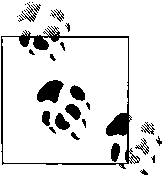
\includegraphics[width=2cm,clip]{paipai.png}
\end{wrapfigure}
\mbox{}POSIX的定时器接口毫无疑问是最先进的,但也是最新的(因而可移植性最差),同时是最不易使用的。如果优先考虑简洁或者可移植性,那么setitimer()是更好的选择。 


\subsubsection{建立一个定时器}

使用timer\_create()建立一个定时器: 

\begin{lstlisting}
  #include <signal.h>
  #include <time.h>

  int timer_create (clockid_t clockid,
		    struct sigevent *evp,
		    timer_t *timerid);
\end{lstlisting}

成功调用timer\_create()建立一个与POSIX时钟clockid相关联的新定时器,在timerid中存储一个唯一的定时器标记,并返回0。该调用很少不会设置定时器运行的条件;就像在下一节将要看到的那样,在启动定时器之前什么都不会发生。 

下面的例子在POSIX时钟CLOCK\_PROCESS\_CPUTIME\_ID上建立了一个新的定时器,并将定时器ID存储到timer中。 

\begin{lstlisting}
  timer_t timer;
  int ret;

  ret = timer_create (CLOCK_PROCESS_CPUTIME_ID,
		      NULL,
		      &timer);
  if (ret)
      perror ("timer_create");
\end{lstlisting}

失败时,调用返回-1,timerid则未定义,调用设置errno为下列值之一:

\begin{eqlist*}
\item [EAGAIN]
系统缺少足够的资源来完成请求。 
\item [EINVAL]
clockid指定的POSIX时钟是非法的。
 \item [ENOTSUP]
clockid指定的POSIX时钟合法,但是系统不支持使用该时钟作为定时器。POSIX保证所有实现均支持CLOCK\_REALTIME时钟作为定时器。其它的时钟是否支持依赖于不同实现。 
\end{eqlist*}

evp参数(非NULL条件下)定义了当定时器到期时的异步通知。头文件<signal.h>定义了该结构体。它的内容对程序员来说是不可见的,但至少包含以下字段: 

\begin{lstlisting}
  #include <signal.h>

  struct sigevent {
      union sigval sigev_value;
      int sigev_signo;
      int sigev_notify;
      void (*sigev_notify_function)(union sigval);
      pthread_attr_t *sigev_notify_attributes;
  };

  union sigval {
      int sival_int;
      void *sival_ptr;
  };
\end{lstlisting}

在基于时钟的POSIX定时器到期时,在内核在如何通知进程的问题上有更多的控制能力,它允许进程指定内核将发送的信号,甚至让内核产生一个新线程在定时器到期时完成一定的功能。进程在定时器过期时的行为通过sigev\_notify来指定,必须是以下三个值之一: 

\begin{eqlist*}
\item [SIGEV\_NONE]
一个“空的”通知。当定时器到期时,什么都不发生。
\item [SIGEV\_SIGNAL]
当定时器到期时,内核给进程发送一个由sigev\_signo指定的信号。在信号处理程序中,si\_value被设置为sigev\_value。 
 \item [SIGEV\_THREAD]
当定时器过期时,内核产生一个新线程(在该进程内),并让其执行sigev\_notify\_function,将sigev\_value做为它唯一的参数。该线程在这个函数返回时终止。如果sigev\_notify\_attributes不是NULL,pthread\_attr\_t结构体则定义了新线程的行为。 
\end{eqlist*}

就像之前的例子中看到的,如果evp是NULL,定时器的到期通知将做如下设置:sigev\_notify为SIGEV\_SIGNAL,sigev\_signo为SIGALRM,sigev\_value 为定时器的ID。就是说,缺省情况下这些定时器以POSIX间歇定时器的方式进行通知。然而通过自定义方式,可以做更多的工作! 

下面的例子建立了一个基于CLOCK\_REALTIME的定时器。当定时器到期时,内核发出SIGUSR1信号,并把si\_value设置成存储定时器ID的地址值: 

\begin{lstlisting}
  struct sigevent evp;
  timer_t timer;
  int ret;

  evp.sigev_value.sival_ptr = &timer;
  evp.sigev_notify = SIGEV_SIGNAL;
  evp.sigev_signo = SIGUSR1;
  ret = timer_create (CLOCK_REALTIME,
		      &evp,
		      &timer);
  if (ret)
      perror ("timer_create");
\end{lstlisting}

\subsection{设置定时器}

由timer\_create()建立的定时器是未设置的。可以使用timer\_settime()将其与一个过期时间关联并开始计时: 

\begin{lstlisting}
  #include <time.h>

  int timer_settime (timer_t timerid,
		     int flags,
		     const struct itimerspec *value,
		     struct itimerspec *ovalue);
\end{lstlisting}

成功调用timer\_settime()将设置timerid指定的定时器的过期时间为value,value为一个timerspec结构体 

\begin{lstlisting}
  struct itimerspec {
      struct timespec it_interval; /* next value */
      struct timespec it_value; /* current value */
  };
\end{lstlisting}

像setitimer()一样,it\_value指定了当前定时器过期时间。当定时器过期时,将用it\_interval的值更新it\_value。如果it\_interval是0,定时器就不是间歇定时器,并在it\_value 过期后停止运行。

回顾一下之前提到的内容,timespec结构体可以提供纳秒级精度:

\begin{lstlisting}
  struct timespec {
      time_t tv_sec; /* seconds */
      long tv_nsec; /* nanoseconds */
  };
\end{lstlisting}

如果flags是TIMER\_ABSTIME,value指定的时间则为绝对时间(和相对于当前时间值的默认解释相反)。这个修正的操作可以避免在获取当前时间、计算相对的时间差值、确定未来时间点、以及设置定时器时产生竞争条件。详情可以参见先前一节“一个高级的睡眠方法”。 

如果ovalue不是NULL,之前定时器的过期时间将存储在itimerspec中。如果定时器之前未被设置,结构体的成员将全部设置为0。 

使用timer值来初始化之前用timer\_create()初始化的定时器,下面的代码建立了一个每秒都过期的周期定时器: 

\begin{lstlisting}
  struct itimerspec ts;
  int ret;

  ts.it_interval.tv_sec = 1;
  ts.it_interval.tv_nsec = 0;
  ts.it_value.tv_sec = 1;
  ts.it_value.tv_nsec = 0;

  ret = timer_settime (timer, 0, &ts, NULL);
  if (ret)
      perror ("timer_settime");
\end{lstlisting}

\subsubsection{取得定时器的过期时间}

你可以在任何时刻使用timer\_gettime()获取一个定时器的过期时间而不必重新设置它: 

\begin{lstlisting}
  #include <time.h>

  int timer_gettime (timer_t timerid,
		     struct itimerspec *value);
\end{lstlisting}

成功调用timer\_gettime()将timerid指定的定时器过期时间存储到value指向的结构体中,并返回0。失败时,调用返回-1,并设置errno为下列值之一: 

\begin{eqlist*}
\item [EFAULT]
value不是合法指针。
\item [EINVAL]
timerid不是合法定时器。 
\end{eqlist*}

看个例子: 

\begin{lstlisting}
  struct itimerspec ts;
  int ret;

  ret = timer_gettime (timer, &ts);
  if (ret)
      perror ("timer_gettime");
  else {
      printf ("current sec=%ld nsec=%ld\n",
      ts.it_value.tv_sec, ts.it_value.tv_nsec);
      printf ("next sec=%ld nsec=%ld\n",
      ts.it_interval.tv_sec, ts.it_interval.tv_nsec);
  }
\end{lstlisting}


\subsubsection{取得定时器的超时值}

POSIX定义了一个接口来确定一个给定定时器目前的超时值: 

\begin{lstlisting}
  #include <time.h>

  int timer_getoverrun (timer_t timerid);
\end{lstlisting}

成功时,timer\_getoverrun()返回在定时器过期与实际定时器过期后通知(例如通过信号)进程间的多余时长。比方说,在我们先前的例子中,一个1毫秒的定时器运行了10毫秒,调用就会返回9。

如果超时值大于等于DELAYTIMER\_MAX,调用就返回DELAYTIMER\_MAX。

失败时,该函数返回-1,并设置errno为EINVAL,这个唯一的错误表明由timerid指定的定时器不合法。

看个例子: 

\begin{lstlisting}
  int ret;

  ret = timer_getoverrun (timer);
  if (ret == -1)
       perror ("timer_getoverrun");
  else if (ret == 0)
      printf ("no overrun\n");
  else
      printf ("%d overrun(s)\n", ret);
\end{lstlisting}

\subsubsection{删除定时器}

删除一个定时器很简单: 

\begin{lstlisting}
  #include <time.h>

  int timer_delete (timer_t timerid);
\end{lstlisting}

成功调用timer\_delete()将销毁由timerid指定的定时器,并返回0。失败时,调用返回-1,并设置errno为EINVAL,这个唯一的错误表明timerid不是合法的定时器。 


%参考文献
% \defaultfont
% \ifx\atempxetex\usewhat
% \bibliographystyle{chinesebst2005_UTF8}
% \else
% \bibliographystyle{chinesebst2005_UTF8}
% \fi
% \addcontentsline{toc}{chapter}{\hei \ReferenceCName}      % 参考文献加入到中文目录
% \addcontentsline{toe}{chapter}{\bfseries \xiaosi \ReferenceEName} % 参考文献加入到英文目录
% \addtolength{\bibsep}{-0.8 em} \nocite{*}
% \bibliography{reference/reference}

%\addtocontents{fen}{\protect\vskip1\baselineskip}
%\addtocontents{ten}{\protect\vskip1\baselineskip}
%英文图形和表格索引里加入空白行,通常放在 % -*-coding: utf-8 -*-

\defaultfont
\appendix

%%%%%%%%%%%%%%%%%%%%%%%%%%%%%%%%%%%%%%%%%%%%%%%%%%%%%%%%%
\BiAppChapter{GCC对C语言的扩展}{}
GCC(GNU编译器集合, GNU Compiler Collection)为C语言提供了多种扩展功能,其中的一些扩展功能对系统程序员尤其有帮助。在本附录所提到的C语言功能扩展中,大多数为编译器提供了关于代码的行为和功能的附加信息。编译器利用这些信息可以产生更高效的机器代码。其他扩展则是对C语言的补充,尤其是在底层的系统调用方面。

最新的C语言标准---ISO C99,包括了GCC所提供的部分扩展功能。有些扩展功能与C99标准中的类似,但另外一些扩展功能在ISO C99中使用了完全不同的实现。新编写的代码应尽量遵循ISO C99标准。在本附录中,我们不会提及此类扩展,而只讨论GCC所特有的扩展功能。

%%%%%%%%%%%%%%%%%%%%%%%%%%%%%%%%%%%%%%%%%%%%%%%%%%%%%%%%%
\BiSection{GNU C}{}
GCC所支持的C语言经常被称为GNU C语言。在90年代,GNU C弥补了C语言本身的一些缺陷,提供了类似于复变量、零长度数组、内联函数、命名初始化等功能。经过十年的发展,C语言标准终于升级到了ISO C99,这导致GNU C的扩展不是很符合新的标准。然而GNU C则持续提供有帮助的特性,许多Linux程序员在其兼容C90或C99标准的代码中,仍然会使用部分GNU C的特性(通常是只使用一两个扩展功能)。

一个典型的使用GCC扩展的例子是Linux的内核,内核代码严格遵照GNU C。最近,Intel花了番功夫对Intel C编译器(ICC, Intel C Compiler)进行改造,使ICC能理解(Linux)内核所使用的那些GNU C扩展。因此,许多扩展已经变得不仅仅是只有GCC才支持了。

\BiSection{内联函数}{}
将函数声明为内联(inline),编译器就会将该函数的整段代码复制到函数的调用地址。编译器直接运行函数本身,而不是将其存储在外部并在调用时跳转至该函数。这样处理既可以省去了函数调用的开销也可以在函数调用地址进行可能的优化(因为编译器能够将调用函数和被调用函数一起进行优化)。当函数的参数在调用时是常量时,后者尤其有效。然而,将函数代码拷贝到每个调用它的地方,必然会增加整体代码长度。因此,只有当函数很小很简单,或者调用次数不是很多的时候,才可以将其声明为内联函数。

GCC支持inline关键字已经很多年了,使用inline就是指示编译器将函数进行内联。C99标准中这样规定inline关键字:
\begin{lstlisting}
	static inline int foo (void) { /* ... */ }
\end{lstlisting}
但从技术上讲,inline关键字只是一种提示,它仅仅是建议编译器对函数进行内联。GCC在此基础上提供了扩展功能,可以指定编译器总是将指定函数进行内联,使用方法如下:

\begin{lstlisting}
	static inline __attribute__ (( always_inline)) int foo (void){ /*...*/ } \right)}
\end{lstlisting}
内联函数的一个显而易见的用途是来替代预处理宏(preprocessor macro)。GCC中的内联函数与宏的行为一样,而且还可以进行类型检查。下面的这个宏:
\begin{lstlisting}
	  #define max(a,b) ({ a > b ? a : b; })
\end{lstlisting}
可以使用以下的内联函数替代:
\begin{lstlisting}
	static inline max (int a, int b)
	{
		if (a > b)
			return a;
		return b;
	}
\end{lstlisting}
程序员一般会过度使用内联函数。在大多数现代的系统架构,尤其是x86上,函数调用的开销非常非常的低。只有在非常需要的情况下才使用内联函数。

\BiSection{禁用内联}{}
在主动优化模式中,GCC会自动选择适合内联的函数,并对其进行内联。一般情况这都是一个不错的处理方式,但有时程序员能判断出函数内联不会正常工作。比如,当使用\verb+__builtin_return_address+时(本附录稍后介绍),内联就可能产生问题。使用noinline可以禁用内联函数:
\begin{lstlisting}
__attribute_ _ ((noinline)) int foo (void) { /* ... */ }
\end{lstlisting}

\BiSection{纯函数}{}
纯函数是指没有任何影响的函数,其返回值仅反映了函数的参数或者非易失(nonvolatile)的全局变量。对于参数或者全局变量的访问必须是只读的。对此类函数可以进行循环优化(loop optimization)和子表达式删除(subexpression elimination)。用pure关键字表明函数为纯函数:
\begin{lstlisting}
    __attribute__ ((pure)) int foo (int val) { /* ... */ }
\end{lstlisting}

常见的例子是strlen()函数。在输入相同的情况下,无论调用多少次,该函数的返回值都保持不变,因此可以从循环中提出来,仅仅调用一次即可。例如,考虑以下代码:
\begin{lstlisting}因为此类函数的返回值是其唯一的出口。
    /* 逐字符地打印数组p中的元素的大写形式 */
    for (i=0; i < strlen (p); i++)
        printf ("%c", toupper (p[i]));
\end{lstlisting}

如果编译器不知道strlen()是纯函数,就可能在每次循环中调用一次该函数!

聪明的程序员会这样改写代码:(如果将strlen()标记为单纯函数,编译器也会按如下代码处理)
\begin{lstlisting}
    size_t len;
    
    len = strlen (p);
    for (i=0; i < len; i++)
        print ("%c", toupper (p[i]));
\end{lstlisting}

附带说一下,更聪明的程序员(比如像本书的读者)还可能会这么做:
\begin{lstlisting}
    while (*p)
        printf ("%c", toupper (*p++));
\end{lstlisting}

因为纯函数的返回值是其唯一的功能,因此让纯函数返回void是非法的,也是没有任何意义的。
\BiSection{常函数}{}
"常函数"是限制更严格的单纯函数。这种函数不访问全局变量,也不能将指针作为参数。因此,常值函数的返回值仅反映以值的方式传进来的参数。除了纯函数的一些优化方式之外,对常函数还可以进行其他优化。数学函数abs()是典型的常函数(假定不进行诸如保存状态或其他假借优化之名所做的小动作)。用const关键字标记常函数:
\begin{lstlisting}
	__attribute__ ((const)) int foo (void) { /* ... */ }
\end{lstlisting}
与纯函数一样,让常值函数返回void也是没有意义的。
\BiSection{不返回的函数}{}
如果函数不返回(比如在函数中调用了exit()),程序员可以用noreturn关键字标记该函数,以此来通知编译器:
\begin{lstlisting}
	__attribute__ ((noreturn)) void foo (int val) { /* ... */ }
\end{lstlisting}
因为无论什么情况下,被调用的函数都不会返回,编译器则可以进行额外的优化。此类函数的返回值只能是void。
\BiSection{分配内存的函数}{}
如果该函数返回指针永远不是已分配内存的别名\footnote{内存别名是指有两个或两个以上的指针指向同一个内存地址。内存别名很常见,比如我们将指针的值赋给另外的指针时,就会产生内存别名。当然,还可能有一些更复杂的情况也会出现内存别名。如果函数返回的是新分配的内存地址,则不会有其他的指针指向同一个内存地址。}(基本可以确认函数分配了新的内存并返回指向新内存的指针),程序员就可以将该函数用malloc标记,而编译器也可以进行适当的优化:
\begin{lstlisting}
    __attribute__ ((malloc)) void * get_page (void)
    {
        int page_size;
        
        page_size = getpagesize ();
        if (page_size <= 0)
            return NULL;
        
        return malloc (page_size);
    }

\end{lstlisting}
\BiSection{强制调用函数检查返回值 }{}
属性\verb+warn_unused_result+可以指示编译器在函数返回值没有保存或没有用在条件语句中时产生警告;这不算是优化,仅是一个辅助功能:
\begin{lstlisting}
    __attribute__ ((warn_unused_result)) int foo (void) { /* ... */ }
\end{lstlisting}
当被调用函数的返回值非常重要的时候,这样处理可以让程序员所有调用函数都检查并处理了返回值。read()一类函数的返回值虽然很重要,但却经常被忽视,这时使用\verb+warn_unused_result+属性再合适不过了。这类函数不能返回void。

\BiSection{将函数标记为deprecated }{}
deprecated属性指示编译器,当函数被调用时产生警告信息:
\begin{lstlisting}
    __attribute__ ((deprecated)) void foo (void) { /* ... */ }
\end{lstlisting}
这有助于提醒程序员不要使用已被弃用或过时的函数。
\BiSection{将函数标记为used}{}
有些情况下,函数会以编译器无法察觉的形式被调用。将函数用used标记可以指示编译器程序中使用了该函数,尽管从表面上看该函数从未被使用:
\begin{lstlisting}
    __attribute__ ((used)) void foo (void) { /* ... */ }
\end{lstlisting}
编译器会输出相应的汇编语言,而且不输出函数未被使用的警告。当静态函数仅被手写的汇编代码调用时,该属性就非常有帮助了。通常情况下(未使用used时),当某函数时没有被调用时,编译器会产生警告,并可能将该函数优化掉。

\BiSection{将函数或参数标记为unused}{}
unused属性指示编译器指定的函数或参数未被使用,并指示编译器不产生相应的警告:
\begin{lstlisting}
     void foo (long __attribute__ ((unused)) value) { /* ... */ }
\end{lstlisting}
这个属性可用于下列情形:使用了-W或-Wunused编译选项,有一些函数必须匹配事先定好的函数签名(这在事件驱动界面编程或者信号处理函数中很常见),而你还想捕捉到真正未使用的函数参数。
\BiSection{将结构体进行打包(pack)}{}
packed属性指示编译器对某类型或变量在内存中以尽可能小的内存空间保存(打包至内存),这个属性潜在的忽略了内存对齐的要求。用该属性限定结构体或联合时,其中的所有变量都会被打包。只限定一个变量时,只有被限定的变量被打包。
下列代码将结构体中的所有变量打包至所需的最小内存空间(1)。
\begin{lstlisting}
     struct __attribute__ ((packed)) foo (void) { ... };
\end{lstlisting}
举例来说,一个结构体含有一个char类型的变量,随后是一个int类型的变量,在编译时通常会将int类型的变量对齐到char类型变量的3个字节之后,而不是将其直接放在char变量的下一个内存地址中。编译器在两个变量之间填充一些不使用的字节,以对变量进行对齐。打包后的结构体不含有这些填充字节,尽可能少的使用些内存,但不满足相应体系结构上的对齐要求。

\BiSection{增加变量的内存对齐量 }{}
除了可以对变量进行打包之外,GCC还允许程序员指定给定变量的最小对齐量。在对该变量进行对齐时,编译器不使用体系结构和ABI所要求的最小对齐量,而是使用不小于该值的对齐量。比如,下列语句声明整型变量\verb+beard_length+,并指定至少进行32个字节的内存对齐(而不是常见的对32位整型变量所进行4字节对齐):

\begin{lstlisting}
    int beard_length __attribute__ ((aligned (32))) = 0;
\end{lstlisting}
通常来讲,强制指定类型的内存对齐量只有在下列情形才能用到:一是硬件的内存对齐要求比体系结构更高,二是在混写C语言和汇编代码中希望使用特定对齐量的语句时。比如说在保存处理器缓存线中经常使用到的变量,以便优化缓存行为时,就可以使用这个功能。Linux内核用到了这种技术。

除了指定最小内存对齐量之外,还可以让GCC将给定变量类型的对齐量设定为所有类型的最小内存对齐量中最大的那个值。下面这代码片段就指定了变量\verb+parrot_height+的内存对齐量为GCC中可以使用的最大值,该值通常是double型:
\begin{lstlisting}
     short parrot_height __attribute__ ((aligned)) = 5;
\end{lstlisting}
如何使用内存对齐量,通常要权衡时间和空间的消耗:经过上述方式对齐的变量会占用更多空间,但是在变量上的复制(以及其他的复杂操作)可能更省时间,因为编译器可以调用处理大块内存的机器指令,以处理大块内存。
体系结构和工具链通常会限制变量所能使用的最大的内存对齐量。在有些Linux体系结构中,链接器仅接受一个相当小的默认的对齐值。这时,使用aligned所指定的对齐量就会被设定为默认值。此外,当你指定变量的对齐量为32个字节,但系统的链接器最多只能对齐8个字节,那么变量就会使用8个字节进行对齐。
\BiSection{将全局变量置于寄存器中 }{}
GCC允许程序员将全局变量放在指定的寄存器中,这样变量将在程序的整个执行期内都处于该寄存器中。GCC中,这样的变量称为“全局寄存器变量”。
语法要求程序员指定具体的寄存器,下面的代码中使用寄存器ebx:
\begin{lstlisting}
    register int *foo asm ("ebx");
\end{lstlisting}

程序员必须保证指定的寄存器不能被函数破坏(function-clobbered):就是说,指定的寄存器必须能被局部函数使用,在函数调用时会进行保存和恢复,而且不能被体系结构或者操作系统的ABI指定用作任何特殊的用途。如果选择的寄存器不合适,编译器就会产生警告信息。要是选择的寄存器合适(本例中使用的ebx在x86架构下就是合适的),编译器就会停止使用该寄存器。
当变量被频繁使用时,将其置于寄存器中可以带来显著的性能提升。虚拟机就是个很好的例子。比如说,将保存虚拟栈帧指针(virtual stack frame pointer)的变量置于寄存器中,将带来很大的好处。另一方面,要是体系结构本身的寄存器就很少(比如像x86中),优化就没什么意义了。
全局寄存器变量不能用于信号处理函数,也不能在多线程程序中使用。这些变量不能设置初始值,因为没有什么机制能让程序为寄存器设定默认值。全局寄存器变量的声明应该位于所有的函数声明之前。
\BiSection{分支预测}{}
GCC允许程序员对表达式的期望值进行预测,比如告诉编译器,条件语句可能是真还是假。相应地,GCC可以对代码块进行顺序调整等优化,这样可以改善条件语句的运行性能。
GCC中,分支预测的语法很难看。为了让分支预测看起来舒服些,使用下列预编译宏:
\begin{lstlisting}
    #define likely(x)    __builtin_expect (!!(x), 1)
    #define unlikely(x)  __builtin_expect (!!(x), 0)
\end{lstlisting}
程序员可以将表达式分别用likely()或者unlikely()括起来,以标记为该表达式“可能为真”或者“不可能为真”。
下列例子标示分支“不可能为真”(也即,“可能为假”)
\begin{lstlisting}
    int ret;
    
    ret = close (fd);

    if (unlikely (ret))
        perror ("close");
\end{lstlisting}
对应的,下列例子标示分支“可能为真”:
\begin{lstlisting}
    const char *home;
    
    home = getenv ("HOME");
    if (likely (home))
        printf ("Your home directory is: %s\n", home);
    else
        fprintf (stderr, "Environment variable HOME not set!\n");
\end{lstlisting}

与内联函数一样,程序员总是倾向于使用过多的分支注解。一旦开始对表达式进行预测,你就可能想去预测所有表达式。当心,只有当你事先知晓,并对表达式在几乎所有的情况下(有99\%的把握)为真或假坚信不疑的情况下,才应该将分支标记为“可能为真”或“不可能为真”。要牢记,错误的预测还不如根本不做预测。
\BiSection{获取表达式的类型}{}
GCC提供关键字typeof,用以取得给定表达式的类型。从语义上看,typeof关键字跟sizeof()的机理相同。比如,下列语句返回x所指向的变量的类型:
\begin{lstlisting}
    typeof (*x)
\end{lstlisting}

可以用下列语句来声明此类型的一个数组y:
\begin{lstlisting}
    typeof (*x) y[42];
\end{lstlisting}

typeof常用来编写“安全”的宏,可以用该宏来操作任意的算术值,而且仅需宏的参数取一次值即可:
\begin{lstlisting}
    #define max(a,b) ({          \
            typeof (a) _a = (a); \
            typeof (b) _b = (b); \
            _a > _b ? _a : _b; \
    })    
\end{lstlisting}
\BiSection{获取类型的内存对齐量}{}
GCC提供关键字\verb+__alignof__+来获取给定对象的对齐量。这个对齐量跟体系结构和ABI都有关。如果当前的体系结构没有提供必需的对齐量,关键字\verb+__alignof__+就返回ABI的推荐对齐量。否则,该关键字返回最小对齐量。
其语法跟sizeof相同:
\begin{lstlisting}
    __alignof__(int)
\end{lstlisting}
依赖于体系结构,上述代码可能返回4,因为32位整型变量通常是按照4个字节的边界进行对齐的。
该关键字还可用于左值。这种情况下,返回的对齐量是相应类型的最小内存对齐量,而不是该左值本身的对齐量。如果用aligned属性修改过最小内存对齐量(在“增加变量的内存对齐量 ”中讨论过),那么该修改可以通过\verb+__alignof__+体现。

比如,考虑以下结构体:
\begin{lstlisting}
    struct ship {
            int year_built;
            char canons;
            int mast_height;
    };
\end{lstlisting}
和下列代码片段:
\begin{lstlisting}
    struct ship my_ship;
    
    printf ("%d\n", __alignof__(my_ship.canons));
\end{lstlisting}
在上述代码中,尽管对于结构体的内存对齐后可能导致canons占用4个字节,但\verb+__alignedof__+表达式将返回1。
\BiSection{ 结构体中成员的偏移量}{}
GCC内置了一个可以获得结构体中某成员在该结构体中的偏移量的关键字。宏offsetof()在\verb+<stddef.h>+中定义,并且是ISO C标准的一部分。大多数的实现都很差劲,这些实现用到了讨厌的指针算术操作,而且代码很难懂。GCC的这个扩展更简单,而且速度可能更快:
\begin{lstlisting}
    #define offsetof(type, member) __builtin_offsetof (type, member)
\end{lstlisting}
上述调用返回了结构体类型type中成员member的偏移量,也就是,从结构体开始到该成员的字节数(从0开始)。例如,考虑下列结构体:
\begin{lstlisting}
    struct rowboat {
        char *boat_name;
        unsigned int nr_oars;
        short length;
    };
\end{lstlisting}
实际的偏移量依赖于变量的大小,以及体系结构的对齐需求和填充行为;但在32位机上,对结构体rowboat和\verb+boat_name、nr_oars、length+调用offsetof(),将分别返回0,4和8。
Linux系统中,宏offsetof()已经定义为GCC的关键字,程序员不必重新定义。
\BiSection{获取函数返回地址}{}
GCC提供一个以获取当前函数(或是当前函数的某个调用者)的返回地址的关键字:
\begin{lstlisting}
    void * __builtin_return_address (unsigned int level)
\end{lstlisting}
参数level指定应该返回函数调用链(call chain)中哪个函数的返回地址。取0,指定的是当前函数(f0)的返回地址;取1,指定的是函数(f0)的调用函数(f1)的返回地址;取2,指定的是调用f1的函数的返回地址;以此类推。
如果当前的函数f0是内联函数,则将返回f1的返回地址。要是觉得不能接受,可以使用\verb+__builtin_return_address+关键字(在“强制禁用内联 {noinline}”中讲过)命令编译器不将该函数作为内联函数处理。
关键字\verb+__builtin_return_address+有几种用途。可以用来调试或提供信息。还可以展开函数调用链,用以实现内部检查、故障信息转储工具(crash dump utility)、调试器等。
注意,有些体系结构只返回当前函数的地址。在这类体系结构中,非0参数可能产生随机的返回值。因此,只有参数是0时才是可移植的,非0值应该只用于调试。

\BiSection{在Case中使用范围}{}
GCC允许在case语句对单独的代码块指定一个值的范围。一般的语法是这样的:
\begin{lstlisting}
    case low ... high:
\end{lstlisting}
比如:
\begin{lstlisting}ospec
    switch (val) {
    case 1 ... 10:
            /* ... */
            break;
    case 11 ... 20:
            /* ... */
            break;
    default:
            /* ... */
    }
\end{lstlisting}
在处理带ASCII码的case语句的范围时,这个功能尤其有用:
\begin{lstlisting}
    case 'A' ... 'Z':
\end{lstlisting}


注意,在省略号前后都有一个空格。不指定空格会把编译器弄糊涂,尤其是当范围是整型值的时候。应该这样写:
\begin{lstlisting}
    case 4 ... 8:
\end{lstlisting}
不要这样写:
\begin{lstlisting}
    case 4...8:
\end{lstlisting}

\BiSection{void和函数指针的算术操作}{}
在GCC中,void类型的指针可以做加减法,函数指针也可以做加减法。正常情况下,ISO C标准是不允许此类指针运算的,因为不存在void指针的大小这个概念,其大小取决于指针真正指向的内容。为了进行这种运算,GCC将指向内容的大小当做是1个字节。这样,下列代码将a增加1:
\begin{lstlisting}
    a++;        /* a 是个void指针 */
\end{lstlisting}
使用编译选项-Wpointer-arith,在用到上述扩展时,GCC就会产生一条警告信息。
\BiSection{让代码变得更美观并有更好的移植性}{}
我们必须承认,\verb+__attribute__+语法不是很美观。为了更好的使用本章中提到的一些扩展,甚至还需要通过预处理宏进行处理。通过调整代码外观,可以对我们使用这些扩展功能有一定的帮助。
通过使用预处理器,很容易达成这个目的。同时,还可以让这些GCC扩展具有更好的可移植性;如果编译器不是GCC(无论此时编译器是什么),那就把这些扩展定义为空。
为了达到这个目的,只需将下列代码放入头文件,并在源文件中引用该头文件:
\begin{lstlisting}
    #if __GUNC__ >= 3
    # undef  inline
    # define inline        inline __attribute ((always_inline))
    # define __noinline    __attribute__ ((noinline))
    # define __pure        __attribute__ ((pure))
    # define __const       __attribute__ ((const))
    # define __noreturn    __attribute__ ((noreturn))
    # define __malloc      __attribute__ ((malloc))
    # define __must_check  __attribute__ ((warn_unused_result))
    # define __deprecated  __attribute__ ((deprecated))
    # define __used        __attribute__ ((used))
    # define __unused      __attribute__ ((unused))
    # define __packed      __attribute__ ((packed))
    # define __align(x)    __attribute__ ((aligned (x)))
    # define __align_max   __attribute__ ((aligned))
    # define likely(x)     __builtin_expect (!!(x), 1)
    # define unlikely(x)   __builtin_expect (!!(x), 0)
    #else
    # define __noinline    /* no noinline */
    # define __pure        /* no pure */
    # define __const       /* no const */
    # define __noreturn    /* no noreturn */
    # define __malloc      /* no malloc */
    # define __must_check  /* no warn_unused_result */
    # define __deprecated  /* no deprecated */
    # define __used        /* no used */
    # define __unused      /* no unused */
    # define __packed      /* no packed */
    # define __align(x)    /* no aligned */
    # define __align_max   /* no aligned_max */
    # define likely(x)     (x)
    # define unlikely(x)   (x)
    #endif
\end{lstlisting}

比如,下列代码以上面定义的简写方式将函数定义为纯函数:
\begin{lstlisting}
    __pure int foo (void) { /* ... */ }
\end{lstlisting}
如果使用GCC编译,函数就被标记上pure属性。如果使用的不是GCC,预编译器将\verb+__pure+标记替换为空(no-op)。需要注意的是,我们可以在定义前指定多种属性,因此同时使用上面的几个定义,也不会有问题。

这样处理之后,代码更容易编写,看起来更漂亮,也有更好的可移植!












% 附录A之前。
%区分开正文和附录的图形和表格,一般没有这个必要。

% -*-coding: utf-8 -*-

\defaultfont
\appendix

%%%%%%%%%%%%%%%%%%%%%%%%%%%%%%%%%%%%%%%%%%%%%%%%%%%%%%%%%
\BiAppChapter{GCC对C语言的扩展}{}
GCC(GNU编译器集合, GNU Compiler Collection)为C语言提供了多种扩展功能,其中的一些扩展功能对系统程序员尤其有帮助。在本附录所提到的C语言功能扩展中,大多数为编译器提供了关于代码的行为和功能的附加信息。编译器利用这些信息可以产生更高效的机器代码。其他扩展则是对C语言的补充,尤其是在底层的系统调用方面。

最新的C语言标准---ISO C99,包括了GCC所提供的部分扩展功能。有些扩展功能与C99标准中的类似,但另外一些扩展功能在ISO C99中使用了完全不同的实现。新编写的代码应尽量遵循ISO C99标准。在本附录中,我们不会提及此类扩展,而只讨论GCC所特有的扩展功能。

%%%%%%%%%%%%%%%%%%%%%%%%%%%%%%%%%%%%%%%%%%%%%%%%%%%%%%%%%
\BiSection{GNU C}{}
GCC所支持的C语言经常被称为GNU C语言。在90年代,GNU C弥补了C语言本身的一些缺陷,提供了类似于复变量、零长度数组、内联函数、命名初始化等功能。经过十年的发展,C语言标准终于升级到了ISO C99,这导致GNU C的扩展不是很符合新的标准。然而GNU C则持续提供有帮助的特性,许多Linux程序员在其兼容C90或C99标准的代码中,仍然会使用部分GNU C的特性(通常是只使用一两个扩展功能)。

一个典型的使用GCC扩展的例子是Linux的内核,内核代码严格遵照GNU C。最近,Intel花了番功夫对Intel C编译器(ICC, Intel C Compiler)进行改造,使ICC能理解(Linux)内核所使用的那些GNU C扩展。因此,许多扩展已经变得不仅仅是只有GCC才支持了。

\BiSection{内联函数}{}
将函数声明为内联(inline),编译器就会将该函数的整段代码复制到函数的调用地址。编译器直接运行函数本身,而不是将其存储在外部并在调用时跳转至该函数。这样处理既可以省去了函数调用的开销也可以在函数调用地址进行可能的优化(因为编译器能够将调用函数和被调用函数一起进行优化)。当函数的参数在调用时是常量时,后者尤其有效。然而,将函数代码拷贝到每个调用它的地方,必然会增加整体代码长度。因此,只有当函数很小很简单,或者调用次数不是很多的时候,才可以将其声明为内联函数。

GCC支持inline关键字已经很多年了,使用inline就是指示编译器将函数进行内联。C99标准中这样规定inline关键字:
\begin{lstlisting}
	static inline int foo (void) { /* ... */ }
\end{lstlisting}
但从技术上讲,inline关键字只是一种提示,它仅仅是建议编译器对函数进行内联。GCC在此基础上提供了扩展功能,可以指定编译器总是将指定函数进行内联,使用方法如下:

\begin{lstlisting}
	static inline __attribute__ (( always_inline)) int foo (void){ /*...*/ } \right)}
\end{lstlisting}
内联函数的一个显而易见的用途是来替代预处理宏(preprocessor macro)。GCC中的内联函数与宏的行为一样,而且还可以进行类型检查。下面的这个宏:
\begin{lstlisting}
	  #define max(a,b) ({ a > b ? a : b; })
\end{lstlisting}
可以使用以下的内联函数替代:
\begin{lstlisting}
	static inline max (int a, int b)
	{
		if (a > b)
			return a;
		return b;
	}
\end{lstlisting}
程序员一般会过度使用内联函数。在大多数现代的系统架构,尤其是x86上,函数调用的开销非常非常的低。只有在非常需要的情况下才使用内联函数。

\BiSection{禁用内联}{}
在主动优化模式中,GCC会自动选择适合内联的函数,并对其进行内联。一般情况这都是一个不错的处理方式,但有时程序员能判断出函数内联不会正常工作。比如,当使用\verb+__builtin_return_address+时(本附录稍后介绍),内联就可能产生问题。使用noinline可以禁用内联函数:
\begin{lstlisting}
__attribute_ _ ((noinline)) int foo (void) { /* ... */ }
\end{lstlisting}

\BiSection{纯函数}{}
纯函数是指没有任何影响的函数,其返回值仅反映了函数的参数或者非易失(nonvolatile)的全局变量。对于参数或者全局变量的访问必须是只读的。对此类函数可以进行循环优化(loop optimization)和子表达式删除(subexpression elimination)。用pure关键字表明函数为纯函数:
\begin{lstlisting}
    __attribute__ ((pure)) int foo (int val) { /* ... */ }
\end{lstlisting}

常见的例子是strlen()函数。在输入相同的情况下,无论调用多少次,该函数的返回值都保持不变,因此可以从循环中提出来,仅仅调用一次即可。例如,考虑以下代码:
\begin{lstlisting}因为此类函数的返回值是其唯一的出口。
    /* 逐字符地打印数组p中的元素的大写形式 */
    for (i=0; i < strlen (p); i++)
        printf ("%c", toupper (p[i]));
\end{lstlisting}

如果编译器不知道strlen()是纯函数,就可能在每次循环中调用一次该函数!

聪明的程序员会这样改写代码:(如果将strlen()标记为单纯函数,编译器也会按如下代码处理)
\begin{lstlisting}
    size_t len;
    
    len = strlen (p);
    for (i=0; i < len; i++)
        print ("%c", toupper (p[i]));
\end{lstlisting}

附带说一下,更聪明的程序员(比如像本书的读者)还可能会这么做:
\begin{lstlisting}
    while (*p)
        printf ("%c", toupper (*p++));
\end{lstlisting}

因为纯函数的返回值是其唯一的功能,因此让纯函数返回void是非法的,也是没有任何意义的。
\BiSection{常函数}{}
"常函数"是限制更严格的单纯函数。这种函数不访问全局变量,也不能将指针作为参数。因此,常值函数的返回值仅反映以值的方式传进来的参数。除了纯函数的一些优化方式之外,对常函数还可以进行其他优化。数学函数abs()是典型的常函数(假定不进行诸如保存状态或其他假借优化之名所做的小动作)。用const关键字标记常函数:
\begin{lstlisting}
	__attribute__ ((const)) int foo (void) { /* ... */ }
\end{lstlisting}
与纯函数一样,让常值函数返回void也是没有意义的。
\BiSection{不返回的函数}{}
如果函数不返回(比如在函数中调用了exit()),程序员可以用noreturn关键字标记该函数,以此来通知编译器:
\begin{lstlisting}
	__attribute__ ((noreturn)) void foo (int val) { /* ... */ }
\end{lstlisting}
因为无论什么情况下,被调用的函数都不会返回,编译器则可以进行额外的优化。此类函数的返回值只能是void。
\BiSection{分配内存的函数}{}
如果该函数返回指针永远不是已分配内存的别名\footnote{内存别名是指有两个或两个以上的指针指向同一个内存地址。内存别名很常见,比如我们将指针的值赋给另外的指针时,就会产生内存别名。当然,还可能有一些更复杂的情况也会出现内存别名。如果函数返回的是新分配的内存地址,则不会有其他的指针指向同一个内存地址。}(基本可以确认函数分配了新的内存并返回指向新内存的指针),程序员就可以将该函数用malloc标记,而编译器也可以进行适当的优化:
\begin{lstlisting}
    __attribute__ ((malloc)) void * get_page (void)
    {
        int page_size;
        
        page_size = getpagesize ();
        if (page_size <= 0)
            return NULL;
        
        return malloc (page_size);
    }

\end{lstlisting}
\BiSection{强制调用函数检查返回值 }{}
属性\verb+warn_unused_result+可以指示编译器在函数返回值没有保存或没有用在条件语句中时产生警告;这不算是优化,仅是一个辅助功能:
\begin{lstlisting}
    __attribute__ ((warn_unused_result)) int foo (void) { /* ... */ }
\end{lstlisting}
当被调用函数的返回值非常重要的时候,这样处理可以让程序员所有调用函数都检查并处理了返回值。read()一类函数的返回值虽然很重要,但却经常被忽视,这时使用\verb+warn_unused_result+属性再合适不过了。这类函数不能返回void。

\BiSection{将函数标记为deprecated }{}
deprecated属性指示编译器,当函数被调用时产生警告信息:
\begin{lstlisting}
    __attribute__ ((deprecated)) void foo (void) { /* ... */ }
\end{lstlisting}
这有助于提醒程序员不要使用已被弃用或过时的函数。
\BiSection{将函数标记为used}{}
有些情况下,函数会以编译器无法察觉的形式被调用。将函数用used标记可以指示编译器程序中使用了该函数,尽管从表面上看该函数从未被使用:
\begin{lstlisting}
    __attribute__ ((used)) void foo (void) { /* ... */ }
\end{lstlisting}
编译器会输出相应的汇编语言,而且不输出函数未被使用的警告。当静态函数仅被手写的汇编代码调用时,该属性就非常有帮助了。通常情况下(未使用used时),当某函数时没有被调用时,编译器会产生警告,并可能将该函数优化掉。

\BiSection{将函数或参数标记为unused}{}
unused属性指示编译器指定的函数或参数未被使用,并指示编译器不产生相应的警告:
\begin{lstlisting}
     void foo (long __attribute__ ((unused)) value) { /* ... */ }
\end{lstlisting}
这个属性可用于下列情形:使用了-W或-Wunused编译选项,有一些函数必须匹配事先定好的函数签名(这在事件驱动界面编程或者信号处理函数中很常见),而你还想捕捉到真正未使用的函数参数。
\BiSection{将结构体进行打包(pack)}{}
packed属性指示编译器对某类型或变量在内存中以尽可能小的内存空间保存(打包至内存),这个属性潜在的忽略了内存对齐的要求。用该属性限定结构体或联合时,其中的所有变量都会被打包。只限定一个变量时,只有被限定的变量被打包。
下列代码将结构体中的所有变量打包至所需的最小内存空间(1)。
\begin{lstlisting}
     struct __attribute__ ((packed)) foo (void) { ... };
\end{lstlisting}
举例来说,一个结构体含有一个char类型的变量,随后是一个int类型的变量,在编译时通常会将int类型的变量对齐到char类型变量的3个字节之后,而不是将其直接放在char变量的下一个内存地址中。编译器在两个变量之间填充一些不使用的字节,以对变量进行对齐。打包后的结构体不含有这些填充字节,尽可能少的使用些内存,但不满足相应体系结构上的对齐要求。

\BiSection{增加变量的内存对齐量 }{}
除了可以对变量进行打包之外,GCC还允许程序员指定给定变量的最小对齐量。在对该变量进行对齐时,编译器不使用体系结构和ABI所要求的最小对齐量,而是使用不小于该值的对齐量。比如,下列语句声明整型变量\verb+beard_length+,并指定至少进行32个字节的内存对齐(而不是常见的对32位整型变量所进行4字节对齐):

\begin{lstlisting}
    int beard_length __attribute__ ((aligned (32))) = 0;
\end{lstlisting}
通常来讲,强制指定类型的内存对齐量只有在下列情形才能用到:一是硬件的内存对齐要求比体系结构更高,二是在混写C语言和汇编代码中希望使用特定对齐量的语句时。比如说在保存处理器缓存线中经常使用到的变量,以便优化缓存行为时,就可以使用这个功能。Linux内核用到了这种技术。

除了指定最小内存对齐量之外,还可以让GCC将给定变量类型的对齐量设定为所有类型的最小内存对齐量中最大的那个值。下面这代码片段就指定了变量\verb+parrot_height+的内存对齐量为GCC中可以使用的最大值,该值通常是double型:
\begin{lstlisting}
     short parrot_height __attribute__ ((aligned)) = 5;
\end{lstlisting}
如何使用内存对齐量,通常要权衡时间和空间的消耗:经过上述方式对齐的变量会占用更多空间,但是在变量上的复制(以及其他的复杂操作)可能更省时间,因为编译器可以调用处理大块内存的机器指令,以处理大块内存。
体系结构和工具链通常会限制变量所能使用的最大的内存对齐量。在有些Linux体系结构中,链接器仅接受一个相当小的默认的对齐值。这时,使用aligned所指定的对齐量就会被设定为默认值。此外,当你指定变量的对齐量为32个字节,但系统的链接器最多只能对齐8个字节,那么变量就会使用8个字节进行对齐。
\BiSection{将全局变量置于寄存器中 }{}
GCC允许程序员将全局变量放在指定的寄存器中,这样变量将在程序的整个执行期内都处于该寄存器中。GCC中,这样的变量称为“全局寄存器变量”。
语法要求程序员指定具体的寄存器,下面的代码中使用寄存器ebx:
\begin{lstlisting}
    register int *foo asm ("ebx");
\end{lstlisting}

程序员必须保证指定的寄存器不能被函数破坏(function-clobbered):就是说,指定的寄存器必须能被局部函数使用,在函数调用时会进行保存和恢复,而且不能被体系结构或者操作系统的ABI指定用作任何特殊的用途。如果选择的寄存器不合适,编译器就会产生警告信息。要是选择的寄存器合适(本例中使用的ebx在x86架构下就是合适的),编译器就会停止使用该寄存器。
当变量被频繁使用时,将其置于寄存器中可以带来显著的性能提升。虚拟机就是个很好的例子。比如说,将保存虚拟栈帧指针(virtual stack frame pointer)的变量置于寄存器中,将带来很大的好处。另一方面,要是体系结构本身的寄存器就很少(比如像x86中),优化就没什么意义了。
全局寄存器变量不能用于信号处理函数,也不能在多线程程序中使用。这些变量不能设置初始值,因为没有什么机制能让程序为寄存器设定默认值。全局寄存器变量的声明应该位于所有的函数声明之前。
\BiSection{分支预测}{}
GCC允许程序员对表达式的期望值进行预测,比如告诉编译器,条件语句可能是真还是假。相应地,GCC可以对代码块进行顺序调整等优化,这样可以改善条件语句的运行性能。
GCC中,分支预测的语法很难看。为了让分支预测看起来舒服些,使用下列预编译宏:
\begin{lstlisting}
    #define likely(x)    __builtin_expect (!!(x), 1)
    #define unlikely(x)  __builtin_expect (!!(x), 0)
\end{lstlisting}
程序员可以将表达式分别用likely()或者unlikely()括起来,以标记为该表达式“可能为真”或者“不可能为真”。
下列例子标示分支“不可能为真”(也即,“可能为假”)
\begin{lstlisting}
    int ret;
    
    ret = close (fd);

    if (unlikely (ret))
        perror ("close");
\end{lstlisting}
对应的,下列例子标示分支“可能为真”:
\begin{lstlisting}
    const char *home;
    
    home = getenv ("HOME");
    if (likely (home))
        printf ("Your home directory is: %s\n", home);
    else
        fprintf (stderr, "Environment variable HOME not set!\n");
\end{lstlisting}

与内联函数一样,程序员总是倾向于使用过多的分支注解。一旦开始对表达式进行预测,你就可能想去预测所有表达式。当心,只有当你事先知晓,并对表达式在几乎所有的情况下(有99\%的把握)为真或假坚信不疑的情况下,才应该将分支标记为“可能为真”或“不可能为真”。要牢记,错误的预测还不如根本不做预测。
\BiSection{获取表达式的类型}{}
GCC提供关键字typeof,用以取得给定表达式的类型。从语义上看,typeof关键字跟sizeof()的机理相同。比如,下列语句返回x所指向的变量的类型:
\begin{lstlisting}
    typeof (*x)
\end{lstlisting}

可以用下列语句来声明此类型的一个数组y:
\begin{lstlisting}
    typeof (*x) y[42];
\end{lstlisting}

typeof常用来编写“安全”的宏,可以用该宏来操作任意的算术值,而且仅需宏的参数取一次值即可:
\begin{lstlisting}
    #define max(a,b) ({          \
            typeof (a) _a = (a); \
            typeof (b) _b = (b); \
            _a > _b ? _a : _b; \
    })    
\end{lstlisting}
\BiSection{获取类型的内存对齐量}{}
GCC提供关键字\verb+__alignof__+来获取给定对象的对齐量。这个对齐量跟体系结构和ABI都有关。如果当前的体系结构没有提供必需的对齐量,关键字\verb+__alignof__+就返回ABI的推荐对齐量。否则,该关键字返回最小对齐量。
其语法跟sizeof相同:
\begin{lstlisting}
    __alignof__(int)
\end{lstlisting}
依赖于体系结构,上述代码可能返回4,因为32位整型变量通常是按照4个字节的边界进行对齐的。
该关键字还可用于左值。这种情况下,返回的对齐量是相应类型的最小内存对齐量,而不是该左值本身的对齐量。如果用aligned属性修改过最小内存对齐量(在“增加变量的内存对齐量 ”中讨论过),那么该修改可以通过\verb+__alignof__+体现。

比如,考虑以下结构体:
\begin{lstlisting}
    struct ship {
            int year_built;
            char canons;
            int mast_height;
    };
\end{lstlisting}
和下列代码片段:
\begin{lstlisting}
    struct ship my_ship;
    
    printf ("%d\n", __alignof__(my_ship.canons));
\end{lstlisting}
在上述代码中,尽管对于结构体的内存对齐后可能导致canons占用4个字节,但\verb+__alignedof__+表达式将返回1。
\BiSection{ 结构体中成员的偏移量}{}
GCC内置了一个可以获得结构体中某成员在该结构体中的偏移量的关键字。宏offsetof()在\verb+<stddef.h>+中定义,并且是ISO C标准的一部分。大多数的实现都很差劲,这些实现用到了讨厌的指针算术操作,而且代码很难懂。GCC的这个扩展更简单,而且速度可能更快:
\begin{lstlisting}
    #define offsetof(type, member) __builtin_offsetof (type, member)
\end{lstlisting}
上述调用返回了结构体类型type中成员member的偏移量,也就是,从结构体开始到该成员的字节数(从0开始)。例如,考虑下列结构体:
\begin{lstlisting}
    struct rowboat {
        char *boat_name;
        unsigned int nr_oars;
        short length;
    };
\end{lstlisting}
实际的偏移量依赖于变量的大小,以及体系结构的对齐需求和填充行为;但在32位机上,对结构体rowboat和\verb+boat_name、nr_oars、length+调用offsetof(),将分别返回0,4和8。
Linux系统中,宏offsetof()已经定义为GCC的关键字,程序员不必重新定义。
\BiSection{获取函数返回地址}{}
GCC提供一个以获取当前函数(或是当前函数的某个调用者)的返回地址的关键字:
\begin{lstlisting}
    void * __builtin_return_address (unsigned int level)
\end{lstlisting}
参数level指定应该返回函数调用链(call chain)中哪个函数的返回地址。取0,指定的是当前函数(f0)的返回地址;取1,指定的是函数(f0)的调用函数(f1)的返回地址;取2,指定的是调用f1的函数的返回地址;以此类推。
如果当前的函数f0是内联函数,则将返回f1的返回地址。要是觉得不能接受,可以使用\verb+__builtin_return_address+关键字(在“强制禁用内联 {noinline}”中讲过)命令编译器不将该函数作为内联函数处理。
关键字\verb+__builtin_return_address+有几种用途。可以用来调试或提供信息。还可以展开函数调用链,用以实现内部检查、故障信息转储工具(crash dump utility)、调试器等。
注意,有些体系结构只返回当前函数的地址。在这类体系结构中,非0参数可能产生随机的返回值。因此,只有参数是0时才是可移植的,非0值应该只用于调试。

\BiSection{在Case中使用范围}{}
GCC允许在case语句对单独的代码块指定一个值的范围。一般的语法是这样的:
\begin{lstlisting}
    case low ... high:
\end{lstlisting}
比如:
\begin{lstlisting}ospec
    switch (val) {
    case 1 ... 10:
            /* ... */
            break;
    case 11 ... 20:
            /* ... */
            break;
    default:
            /* ... */
    }
\end{lstlisting}
在处理带ASCII码的case语句的范围时,这个功能尤其有用:
\begin{lstlisting}
    case 'A' ... 'Z':
\end{lstlisting}


注意,在省略号前后都有一个空格。不指定空格会把编译器弄糊涂,尤其是当范围是整型值的时候。应该这样写:
\begin{lstlisting}
    case 4 ... 8:
\end{lstlisting}
不要这样写:
\begin{lstlisting}
    case 4...8:
\end{lstlisting}

\BiSection{void和函数指针的算术操作}{}
在GCC中,void类型的指针可以做加减法,函数指针也可以做加减法。正常情况下,ISO C标准是不允许此类指针运算的,因为不存在void指针的大小这个概念,其大小取决于指针真正指向的内容。为了进行这种运算,GCC将指向内容的大小当做是1个字节。这样,下列代码将a增加1:
\begin{lstlisting}
    a++;        /* a 是个void指针 */
\end{lstlisting}
使用编译选项-Wpointer-arith,在用到上述扩展时,GCC就会产生一条警告信息。
\BiSection{让代码变得更美观并有更好的移植性}{}
我们必须承认,\verb+__attribute__+语法不是很美观。为了更好的使用本章中提到的一些扩展,甚至还需要通过预处理宏进行处理。通过调整代码外观,可以对我们使用这些扩展功能有一定的帮助。
通过使用预处理器,很容易达成这个目的。同时,还可以让这些GCC扩展具有更好的可移植性;如果编译器不是GCC(无论此时编译器是什么),那就把这些扩展定义为空。
为了达到这个目的,只需将下列代码放入头文件,并在源文件中引用该头文件:
\begin{lstlisting}
    #if __GUNC__ >= 3
    # undef  inline
    # define inline        inline __attribute ((always_inline))
    # define __noinline    __attribute__ ((noinline))
    # define __pure        __attribute__ ((pure))
    # define __const       __attribute__ ((const))
    # define __noreturn    __attribute__ ((noreturn))
    # define __malloc      __attribute__ ((malloc))
    # define __must_check  __attribute__ ((warn_unused_result))
    # define __deprecated  __attribute__ ((deprecated))
    # define __used        __attribute__ ((used))
    # define __unused      __attribute__ ((unused))
    # define __packed      __attribute__ ((packed))
    # define __align(x)    __attribute__ ((aligned (x)))
    # define __align_max   __attribute__ ((aligned))
    # define likely(x)     __builtin_expect (!!(x), 1)
    # define unlikely(x)   __builtin_expect (!!(x), 0)
    #else
    # define __noinline    /* no noinline */
    # define __pure        /* no pure */
    # define __const       /* no const */
    # define __noreturn    /* no noreturn */
    # define __malloc      /* no malloc */
    # define __must_check  /* no warn_unused_result */
    # define __deprecated  /* no deprecated */
    # define __used        /* no used */
    # define __unused      /* no unused */
    # define __packed      /* no packed */
    # define __align(x)    /* no aligned */
    # define __align_max   /* no aligned_max */
    # define likely(x)     (x)
    # define unlikely(x)   (x)
    #endif
\end{lstlisting}

比如,下列代码以上面定义的简写方式将函数定义为纯函数:
\begin{lstlisting}
    __pure int foo (void) { /* ... */ }
\end{lstlisting}
如果使用GCC编译,函数就被标记上pure属性。如果使用的不是GCC,预编译器将\verb+__pure+标记替换为空(no-op)。需要注意的是,我们可以在定义前指定多种属性,因此同时使用上面的几个定义,也不会有问题。

这样处理之后,代码更容易编写,看起来更漂亮,也有更好的可移植!












            % 附录A
\BiAppChapter{参考书目}{}
这份书目包括了系统编程相关的推荐读物,分为四个部分进行介绍。阅读本书时并不需要读这些著作。它们是我认为在相关主题上最好的书。如果你希望深入了解某些主题,我强烈推荐这些书。

部分书籍所讨论的内容是假设本书的读者已经熟悉的(例如C语言)。某些则是对本书的有效补充,例如介绍gdb,Subversion(svn),以及操作系统设计方面的书籍。另外一些所讨论的问题超出了本书的范围(例如套接字的多线程编程)。无论其内容如何,我向大家推荐所有的书。当然,这份书单算不上详尽——你可以自由选择其他读物。

\BiSection{C语言程序设计的相关书籍}{}
以下书籍介绍了系统编程的通用语言--- C语言。如果你不能熟练地编写C语言代码,以下的书籍(辅以大量的练习!)应该能在这方面提供帮助。至少,第一本——以K\&R而广为人知——是非常适合阅读的。它简短的篇幅很好的体现了C语言的简单性。

\textit{The C Programming Language}, 2nd ed. Brian W. Kernighan and Dennis M. Ritchie.
    Prentice Hall, 1988.
    这本书由C程序设计语言的作者和他的伙伴所著,被称作C语言圣经。

\textit{C in a Nutshell}. Peter Prinz and Tony Crawford. O’Reilly Media, 2005.
    一本很好的关于C语言和C标准库的书籍。
\textit{C Pocket Reference}. Peter Prinz and Ulla Kirch-Prinz. Translated by Tony Crawford.
    O’Reilly Media, 2002.
    一份简明扼要的C语言参考,已经更新到最新的ANSI C99标准。
\textit{Expert C Programming}. Peter van der Linden. Prentice Hall, 1994.
    该书对C语言中较少为人所知的部分进行了一次精彩讨论,行文中闪现着作者令人惊奇的才智和幽默感。该书充满了无厘头的笑话,不过我喜欢。
\textit{C Programming FAQs: Frequently Asked Questions}, 2nd ed. Steve Summit. Addison-Wesley, 1995.
    
    这本大部头囊括了超过400个C程序设计语言的常见问题(包括答案)。许多FAQ在C语言专家眼中是小菜一碟,但对于一些重要问题的问答,即使是最博学的C程序员都会被雷到。如果你能解决所有这些“怪物”,你绝对是一个C语言忍者!该书唯一不足就没有跟上ANSI C99,而这肯定会带来一些变化(我在自己手头的书中已经做了修正)。需要注意的是,有一份在线版本的貌似已经做了更新。

\BiSection{Linux编程的相关书籍}{}
下面推荐的书籍主要介绍Linux编程的相关主题,其中包括了本书没有讨论的主题(套接字,IPC,以及pthreads),和Linux编程工具(CVS,GNU Make,以及Subversion)。

\textit{Unix Network Programming, Volume 1: The Sockets Networking API}, 3rd ed. W. Rich-
    ard Stevens et al. Addison-Wesley, 2003.
    套接字API的绝对巨著;可惜并不是针对Linux的,不过最近更新到了IPv6。

\textit{UNIX Network Programming, Volume 2: Interprocess Communications}, 2nd ed.
   W. Richard Stevens. Prentice Hall, 1998.
    关于进程间通信(IPC)的绝佳讨论。

\textit{PThreads Programming: A POSIX Standard for Better Multiprocessing}. Bradford
   Nichols et al. O’Reilly Media, 1996.
    关于POSIX线程API---pthreads的评述。

\textit{Managing Projects with GNU Make}, 3rd ed. Robert Mecklenburg. O’Reilly Media,
   2004.
    关于GNU Make---Linux上建立软件项目的经典工具的绝佳描述。

\textit{Essential CVS}, 2nd ed. Jennifer Versperman. O’Reilly Media, 2006.
    关于CVS---Unix系统上版本控制和源码管理的经典工具的绝佳描述。

\textit{Version Control with Subversion}. Ben Collins-Sussman et al. O’Reilly Media, 2004.
    关于Subversion---Unix系统上版本控制和源码管理的优秀工具的令人惊奇的叙述,由Subversion的三位作者完成。

\textit{GDB Pocket Reference}. Arnold Robbins. O’Reilly Media, 2005.
    一份gdb---Linux调试器的袖珍指南。

\textit{Linux in a Nutshell}, 5th ed. Ellen Siever et al. O’Reilly Media, 2005.
    对Linux中各种内容的快速浏览,包括许多Linux开发环境下的工具。

\BiSection{Linux内核的相关书籍}{}
下面列出的两本书主要涉及Linux内核方面的主题。我们有三重理由来对该主题进行研究。首先,内核提供了对用户空间的系统调用接口。其次,内核的行为和特性会在与其上运行的应用进行交互时体现出来。最后,Linux内核代码非常优美,同时这些书很有意思。

\textit{Linux Kernel Development}, 2nd ed. Robert Love. Novell Press, 2005.
    该书非常适合给那些希望了解Linux内核设计实现的系统程序员阅读(很显然,我就不必提及我在该主题上的看法了)。该书不仅可作为API参考,同时也对Linux内核中使用的算法以及所做的决策也做了精彩的论述。
\textit{Linux Device Drivers}, 3rd ed. Jonathan Corbet et al. O’Reilly Media, 2005.
    本书是在编写Linux内核设备驱动程序方面的绝佳指南,同时也是非常棒的API参考手册。尽管针对的是设备驱动,但书中的讨论可以使各类程序员受益(包括很少探究Linux内核机制的系统程序员)。该书是我在Linux内核方面的必备书籍。

\BiSection{操作系统设计的相关书籍}{}
这两本书不是针对Linux的,而是从理论上介绍操作系统设计与实现。正如我在本书所强调的那样,对你进行编程其上的系统有一个良好的认识颇有助益。

\textit{Operating Systems}, 3rd ed. Harvey Deitel et al. Prentice Hall, 2003.
    操作系统设计理论方面的力作,同时还包括将理论付诸实践的顶尖样例分析。在所有操作系统设计书籍中,这是我的最爱:它紧随操作系统的研究发展,易读且详尽。

\textit{UNIX Systems for Modern Architectures: Symmetric Multiprocessing and Caching for Kernel Programming}. Curt Schimmel. Addison-Wesley, 1994.
   
    尽管和系统编程的关系不大,但该书为并发的危险性和现代缓存系统提供了绝佳的描述。吐血推荐!



     % 参考文献
% % -*-coding: utf-8 -*-

\defaultfont
\BiAppendixChapter{攻读\cxuewei 学位期间发表的学术论文及其它成果} {Papers
Published in the Period of PH. D. Education}

% 书写格式与参考文献相同,这里手写吧 :-)
% 参见...\Accessories\ThesisCriterion\参考文献国标GB7714-2005.pdf内规定
(一)发表的学术论文
\begin{publist}
\item 作者. 题目. 期刊. 年, 卷(期): 页码

\item 作者. 题目. 期刊. 年, 卷(期): 页码

\item 作者. 题目. 期刊. 年, 卷(期): 页码
\end{publist}

(二)申请及已获得的专利(无专利时此项可以不列出)


(三)获得的科技奖励(无获奖时此项不必列出)


% 注:
% 如已发表的学术论文被EI或SCI收录,请标明收录号及SCI论文的影响因子;
% 对已接收但尚未发表出来的学术论文,请注明是否EI或SCI刊源。




    % 所发文章
% % -*-coding: utf-8 -*-

% 先后有三个版本的 授权书格式


\iffalse   %注释掉第一个,采用第二个;
%  +++++++++ 下面是第一种处理方式  ++++++++++++++++++++++++++
    \newpage
%%%%%%%%%%%%%%%%%%哈尔滨工业大学博(硕)士学位论文原创性声明%%%%%%%%%%%%%%%%%%%
    \BiAppendixChapter{哈尔滨工业大学\cxuewei 学位论文原创性声明}{Statement of Copyright}

    本人郑重声明: 此处所提交的 \cxuewei 学位论文《\chinesethesistitle》,
    是本人在导师指导下, 在哈尔滨工业大学攻读\cxuewei 学位期间独立进行研究工作所取得的成果。据本人所知,论文中除已注明部分外不包含他人已发表或撰写过的研究成果。
    对本文的研究工作做出重要贡献的个人和集体, 均已在文中以明确方式注明。 本声明的
    法律结果将完全由本人承担。
    \vspace{0.5cm}
    \begin{flushright}{
    作者签名:~~~~~~~~~~~~~~~~~~~~~~~~~~~~~~~日期:~~~~~~~~~~~年~~~~~月~~~~~日}
    \end{flushright}

    \vspace{0.3cm}

%%%%%%%%%%%%%%%%%%哈尔滨工业大学博(硕)士学位论文使用授权书%%%%%%%%%%%%%%%%%%%
%\phantomsection
\addcontentsline{toc}{chapter}{\hei 哈尔滨工业大学\cxuewei 学位论文使用授权书}
\addcontentsline{toe}{chapter}{\bfseries\xiaosi Letter of Authorization}
    \begin{center}{\xiaoer \hei \bfseries
                    哈尔滨工业大学\cxuewei 学位论文使用授权书}
    \end{center}

    \vspace{0.4cm}

《\chinesethesistitle》 系本人在哈尔滨工业大学攻读\cxuewei 学位期
间在导师指导下完成的\cxuewei 学位论文。本论文的研究成果归哈尔滨工业大学所有,本
论文的研究内容不得以其它单位的名义发表。本人完全了解哈尔滨工业大学关于保存
、使用学位论文的规定,同意学校保留并向有关部门送交论文的复印件和电子版本,
允许论文被查阅和借阅,同意学校将论文加入《中国优秀博硕士学位论文全文数据库》和编入《中国知识资源总库》。本人授权哈尔滨工业大学,可以采用影印、缩印或其他复制
手段保存论文,可以公布论文的全部或部分内容。

\vspace{1.0cm}
\begin{flushright}{
作者签名:~~~~~~~~~~~~~~~~~~~~~~~~~~~~~~~日期:~~~~~~~~~~~年~~~~~月~~~~~日}
\end{flushright}
\vspace{0.2cm}
\begin{flushright}{
导师签名:~~~~~~~~~~~~~~~~~~~~~~~~~~~~~~~日期:~~~~~~~~~~~年~~~~~月~~~~~日}
\end{flushright}

\newpage

\BiAppendixChapter{哈尔滨工业大学\cxuewei 学位涉密论文管理}{Letter of Secret}

%    \begin{center}{\xiaoer \hei \bfseries
%                    哈尔滨工业大学硕博士学位涉密论文管理}
%    \end{center}
%    \vspace{0.4cm}
%\addcontentsline{toc}{chapter}{\hei 哈尔滨工业大学\cxuewei 学位涉密论文管理}
%\addcontentsline{toe}{chapter}{\bfseries\xiaosi Letter of Secret}

根据《哈尔滨工业大学关于国家秘密载体保密管理的规定》,毕业论文答辩必须由导师进行保密初审,外寄论文由科研处复审。涉密毕业论文,由学生按学校规定的统一程序在导师指导下填报密级和保密期限。

 \vspace{0.5cm}
~~~~~~~~~~~~~~~~~~~~~~~~~~~~~~~保密$\square$,在~~~~年解密后适用本授权书。

本学位论文属于

~~~~~~~~~~~~~~~~~~~~~~~~~~~~~~不保密 $\square$ 。

(请在以上相应方框内打“$\surd$”)
\vspace{1.0cm}

\begin{flushright}{
作者签名:~~~~~~~~~~~~~~~~~~~~~~~~~~~~~~~日期:~~~~~~~~~~~年~~~~~月~~~~~日}
\end{flushright} %\vspace{0.2cm}
\begin{flushright}{
导师签名:~~~~~~~~~~~~~~~~~~~~~~~~~~~~~~~日期:~~~~~~~~~~~年~~~~~月~~~~~日}
\end{flushright}

\fi  %注释掉第一个,采用第二个;

%+++++++++++++++++++++++第二种处理方式 by pineapple ++++++++++++++++++++++++++++++++
 \iffalse %% 如果不使用这种方式,去掉 \iffalse \fi 前面的注释
%%%%%%%%%%%%%%%%%%%%%%%%%%%%%%%%%%%%%%%%%%%%%%%%%%%%%%%%%%%%%%%%%%%%%%%%%%%%%%%%
% authorization.tex
%
% Authorization for Use with the Pluto Master Template
%
% Copyright (C) 2006 LIU Yu <pineapple.liu@gmail.com>
%
% This work may be distributed and/or modified under the conditions of the LaTeX
% Project Public License, either version 1.3 of this license or (at your option)
% any later version.
% The latest version of this license is in
%   http://www.latex-project.org/lppl.txt
% and version 1.3 or later is part of all distributions of LaTeX version
% 2005/12/01 or later.
%
% This work has the LPPL maintenance status `unmaintained'.
%
% This work consists of the file(s) authorization.tex
%%%%%%%%%%%%%%%%%%%%%%%%%%%%%%%%%%%%%%%%%%%%%%%%%%%%%%%%%%%%%%%%%%%%%%%%%%%%%%%%

\newpage
\markboth{哈尔滨工业大学\cxuewei 学位论文原创性声明}{哈尔滨工业大学\cxueke\cxuewei 学位论文}

\vspace*{0.1cm}
\newcommand{\subchapterstyle}%
  {\CJKfamily{hei}\rmfamily\bfseries\fontsize{16bp}{16bp}\selectfont}

%\phantomsection
\addcontentsline{toc}{chapter}{\hei 哈尔滨工业大学\cxuewei 学位论文原创性声明}
\addcontentsline{toe}{chapter}{\bfseries\xiaosi Statement of Copyright}
\begin{center}{\subchapterstyle 哈尔滨工业大学\cxuewei 学位论文原创性声明}\end{center}

    本人郑重声明:此处所提交的\cxuewei 学位论文《\chinesethesistitle》 ,是本人在导师指导下,在哈尔滨工业大学攻读\cxuewei 学位期间独立进行研究工作所取得的成果。据本人所知,论文中除已注明部分外不包含他人已发表或撰写过的研究成果。对本文的研究工作做出重要贡献的个人和集体,均已在文中以明确方式注明。本声明的法律结果将完全由本人承担。

\begin{flushright}

作者签字:~~~~~~~~~~~~~~~~~~~~~~~~~~~~~~~~~~~日期:~~~~~~~~~年~~~~~~月~~~~~~日~~~~

\end{flushright}

%\phantomsection
\addcontentsline{toc}{chapter}{\hei 哈尔滨工业大学\cxuewei 学位论文使用授权书}
\addcontentsline{toe}{chapter}{\bfseries\xiaosi Letter of Authorization}
\begin{center}{\subchapterstyle 哈尔滨工业大学\cxuewei 学位论文使用授权书}\end{center}

    《\chinesethesistitle》 系本人在哈尔滨工业大学攻读\cxuewei 学位期间在导师指导下完成的\cxuewei 学位论文。本论文的研究成果归哈尔滨工业大学所有,本论文的研究内容不得以其它单位的名义发表。本人完全了解哈尔滨工业大学关于保存、使用学位论文的规定,同意学校保留并向有关部门送交论文的复印件和电子版本,允许论文被查阅和借阅,同意学校将论文加入《中国优秀博硕士学位论文全文数据库》和编入《中国知识资源总库》。本人授权哈尔滨工业大学,可以采用影印、缩印或其他复制手段保存论文,可以公布论文的全部或部分内容。

\begin{flushright}

作者签名:~~~~~~~~~~~~~~~~~~~~~~~~~~~~~~~~~~~日期:~~~~~~~~~年~~~~~~月~~~~~~日~~~~

导师签名:~~~~~~~~~~~~~~~~~~~~~~~~~~~~~~~~~~~日期:~~~~~~~~~年~~~~~~月~~~~~~日~~~~

\end{flushright}

%\phantomsection
\addcontentsline{toc}{chapter}{\hei 哈尔滨工业大学\cxuewei 学位涉密论文管理} %研究生院说明:暂时不要添加到目录中去,
\addcontentsline{toe}{chapter}{\bfseries\xiaosi Letter of Secret}              %格式也没有完全规定,这里放到下一页上。

\begin{center}{\subchapterstyle 哈尔滨工业大学\cxuewei 学位涉密论文管理}\end{center}

    根据《哈尔滨工业大学关于国家秘密载体保密管理的规定》,毕业论文答辩必须由导师进行保密初审,外寄论文由科研处复审。涉密毕业论文,由学生按学校规定的统一程序在导师指导下填报密级和保密期限。

\begin{flushright}

本学位论文属于~~~~~~~~~~~~~~~~~~~保密$\square$,在~~~~~~~~~~~~年解密后适用本授权书。~~~~~

不保密
$\square$。~~~~~~~~~~~~~~~~~~~~~~~~~~~~~~~~~~~~~~~~~~~~~~~~~~~~~~~~~~~~~~

(请在以上相应方框内打“$\surd$”)~~~~~~~~~~~~~~~~~~~~~~~~~~~~~~~~~~~~~~~~~~~~~~~~~~~~~~~~~~~~~~~~~~~~~~~

\end{flushright}
\begin{flushright}

作者签名:~~~~~~~~~~~~~~~~~~~~~~~~~~~~~~~~~~~日期:~~~~~~~~~年~~~~~~月~~~~~~日~~~~

导师签名:~~~~~~~~~~~~~~~~~~~~~~~~~~~~~~~~~~~日期:~~~~~~~~~年~~~~~~月~~~~~~日~~~~

\end{flushright}
 \fi

%% 第三种处理方式  author: jdg
% \iffalse
\newpage
\markboth{哈尔滨工业大学\cxuewei 学位论文原创性声明}{哈尔滨工业大学\cxueke\cxuewei 学位论文}

\vspace*{0cm}
\newcommand{\subchapterstyle}%
  {\CJKfamily{hei}\rmfamily\bfseries\fontsize{16bp}{16bp}\selectfont}

%\phantomsection
\addcontentsline{toc}{chapter}{\hei 哈尔滨工业大学\cxuewei 学位论文原创性声明}
\addcontentsline{toe}{chapter}{\bfseries\xiaosi Statement of Copyright}
\begin{center}{\subchapterstyle 哈尔滨工业大学\cxuewei 学位论文原创性声明}\end{center}

    本人郑重声明:此处所提交的\cxuewei 学位论文《\chinesethesistitle》 ,是本人在导师指导下,在哈尔滨工业大学攻读\cxuewei 学位期间独立进行研究工作所取得的成果。据本人所知,论文中除已注明部分外不包含他人已发表或撰写过的研究成果。对本文的研究工作做出重要贡献的个人和集体,均已在文中以明确方式注明。本声明的法律结果将完全由本人承担。

\begin{flushright}

作者签名:~~~~~~~~~~~~~~~~~~~~~~~~~~~~~~~~~~~日期:~~~~~~~~~年~~~~~~月~~~~~~日~~~~

\end{flushright}

\vspace{0.4cm}
%\phantomsection
\addcontentsline{toc}{chapter}{\hei 哈尔滨工业大学\cxuewei 学位论文使用授权书}
\addcontentsline{toe}{chapter}{\bfseries\xiaosi Letter of Authorization}
\begin{center}{\subchapterstyle 哈尔滨工业大学\cxuewei 学位论文使用授权书}\end{center}

    《\chinesethesistitle》 系本人在哈尔滨工业大学攻读\cxuewei 学位期间在导师指导下完成的\cxuewei 学位论文。本论文的研究成果归哈尔滨工业大学所有,本论文的研究内容不得以其它单位的名义发表。本人完全了解哈尔滨工业大学关于保存、使用学位论文的规定,同意学校保留并向有关部门送交论文的复印件和电子版本,允许论文被查阅和借阅,同意学校将论文加入《中国优秀博硕士学位论文全文数据库》和编入《中国知识资源总库》。本人授权哈尔滨工业大学,可以采用影印、缩印或其他复制手段保存论文,可以公布论文的全部或部分内容。

\vspace{0.6cm}
本学位论文属于(请在以下相应方框内打“$\surd$”):

保密$\square$,在~~~~~~~~~~~~~年解密后适用本授权书

不保密$\square$

\begin{flushright}{
作者签名:~~~~~~~~~~~~~~~~~~~~~~~~~~~~~~~~~~~日期:~~~~~~~~~年~~~~~~月~~~~~~日~~~~}
\end{flushright} %\vspace{0.2cm}
\begin{flushright}{
导师签名:~~~~~~~~~~~~~~~~~~~~~~~~~~~~~~~~~~~日期:~~~~~~~~~年~~~~~~月~~~~~~日~~~~}
\end{flushright}
%\fi   % 承诺
% % -*-coding: utf-8 -*-

\defaultfont

\BiAppendixChapter{致~~~~谢}{Acknowledgements}

该论文模板是UFO@bbs.hit.edu.cn的《哈尔滨工业大学大学博士(硕士)论文模板》的基础上,
并在很多人的帮助下完成的,在此一并向他们表示感谢。

特别感谢Stanley创立了论文模板开源项目Pluto以及他对论文模板的大量修改,
使之更加符合工大论文模板要求。

特别感谢哈工大紫丁香站的~Tex~的版主~Tex、nebula和网友cucme,
他们自始至终都全力支持模板的制作,并为此作了大量的工作。

感谢邓年春~(HIT bbs ID: dengnch),他花了大量的时间来精调模板的
一系列参数,使得该~\LaTeX~模板和对应的~Word~模板的格式几乎完全一致。

感谢水木清华的~\TeX~和~\LaTeX~版的各位网友为我提供的各种帮助,
特别是~snoopyzhao~网友,他多次热心地为该模板解决各种困难,使得模板的制作得以
顺利进行。

最后,衷心感谢哈工大紫丁香~bbs~站~Tex~版所有网友的大力支持!



值此论文完成之际,谨向给予我无私帮助的老师和同学们致以诚挚的谢意!

首先感谢我的导师{\bf 某某某}教授,本论文的研究工作正是在{\bf
某}老师最初的建议下展开的。
他在学术上不断进取、对人生理想执着追求的精神是我学习的榜样。{\bf
某}老师对问题深刻的认识和深入浅出的讲解给我留下深刻印象。


感谢{\bf 某某某}教授和{\bf 某某某}教授对我学习和工作的帮助,
他们勤奋的工作作风、达观的人生态度都深深地感染了我。感谢{\bf
某某某}教授和{\bf 某某某}教授对我学业和生活上的关心。


感谢博士生{\bf 某某某}、{\bf 某某某}、{\bf 某某某}、{\bf 某某某},
给我的无私帮助和积极支持。感谢实验室所有的兄弟姐妹们,
陪伴我度过了这长久的学习、研究阶段,帮助我解决问题,开拓思想。

最后,特别要感谢我的亲人们,他们对我要求甚少,但给予我的都是关怀、支持和理解。
% 致谢
% % -*-coding: utf-8 -*-

\defaultfont

\BiAppendixChapter{个人简历}{Resume}

{\hei 学习经历}
\begin{publist}
\item xxxx~年~x~月--至今~~哈尔滨工业大学xxxxxxxxx系~~~攻读工学博士学位
\item xxxx~年~x~月~~~xxxxxxx大学xxxxxxxxxxxxxxxxxx系~~~获工学硕士学位
\item xxxx~年~x~月~~~xxxxxxx大学xxxxxxxxxxxxxxxxxx系~~~获工学学士学位
\end{publist}

{\hei 工作经历}
\begin{publist}
\item xxxx~年~x~月--xxxx~年~x~月  单位  职务
\item xxxx~年~x~月--xxxx~年~x~月  单位  职务
\end{publist}

{\hei 科研工作}
\begin{publist}
\item  xxxx~年~x~月--xxxx~年~x~月 ~~~ xxxx项目~~~~(编号xxx-xxx-xxx) 
\item  xxxx~年~x~月--xxxx~年~x~月 ~~~ xxxx项目~~~~(编号xxx-xxx-xxx)
\item  xxxx~年~x~月--xxxx~年~x~月 ~~~ xxxx项目~~~~(编号xxx-xxx-xxx)
\item  xxxx~年~x~月--xxxx~年~x~月 ~~~ xxxx项目~~~~(编号xxx-xxx-xxx)
\end{publist}

{\hei 学术论文}
\begin{publist}
\item 在~xxxxxxx~等刊物发表论文多篇
\item 在~xxxxxxxxxxxxxxxx~等多个国际会议上发表论文多篇
\end{publist}

{\hei 专利情况}
\begin{publist}
\item 作者. 产品名称. 专利名称(专利号:XXXXXXX), 年。
\item 作者. 产品名称. 专利名称(专利号:XXXXXXX), 年。
\end{publist}
          % 个人简历

\clearpage
\ifx\atempxetex\usewhat\else
\end{CJK*}
\fi

\end{document}

%%% Local Variables: 
%%% mode: latex
%%% TeX-master: t
%%% End: 
